\documentclass[11pt,openright,twoside]{book}

% ==============================================================================
% Preamble for "Hydra: Design and Implementation"
% Modernized textbook style inspired by Prentice Hall & Tanenbaum
% ==============================================================================

\usepackage[utf8]{inputenc}
\usepackage[T1]{fontenc}
\usepackage{lmodern}
\usepackage{microtype}

% Geometry & Margins
\usepackage[
    paper=letterpaper,
    top=1.0in,
    bottom=1.0in,
    inner=1.1in,
    outer=0.9in,
    headheight=14pt,
    headsep=20pt,
    footskip=30pt
]{geometry}

% Math & Symbols
\usepackage{amsmath,amssymb,amsfonts}
\usepackage{bm}

% Graphics, Colors & Diagrams
\usepackage{graphicx}
\usepackage{xcolor}
\usepackage{tikz}
\usetikzlibrary{shapes,arrows.meta,positioning,calc,fit,backgrounds,matrix,chains}

% Palette
\definecolor{hydrablue}{RGB}{18, 52, 86}
\definecolor{hydragold}{RGB}{212, 143, 24}
\definecolor{hydragray}{RGB}{60, 64, 67}
\definecolor{hydralight}{RGB}{245, 247, 250}
\definecolor{codebg}{RGB}{248, 249, 250}
\definecolor{codeborder}{RGB}{218, 222, 228}
\definecolor{rustred}{RGB}{183, 65, 14}
\definecolor{rustkeyword}{RGB}{14, 110, 184}
\definecolor{rustcomment}{RGB}{108, 117, 125}
\definecolor{ruststring}{RGB}{40, 138, 48}

% Headers & Footers
\usepackage{fancyhdr}
\pagestyle{fancy}
\fancyhf{}
\fancyhead[LE]{\small\bfseries\color{hydrablue}\thepage\quad\textbar\quad\nouppercase{\leftmark}}
\fancyhead[RO]{\small\bfseries\color{hydrablue}\nouppercase{\rightmark}\quad\textbar\quad\thepage}
\renewcommand{\headrulewidth}{0.4pt}
\renewcommand{\footrulewidth}{0pt}

% Section Titles
\usepackage{titlesec}
\titleformat{\chapter}[display]
  {\normalfont\sffamily\huge\bfseries\color{hydrablue}}
  {\Large\textsc{\chaptertitlename\ \thechapter}}
  {10pt}
  {\titlerule[1.5pt]\vspace{6pt}\Huge}
\titlespacing*{\chapter}{0pt}{10pt}{30pt}

\titleformat{\section}
  {\normalfont\sffamily\Large\bfseries\color{hydrablue}}
  {\thesection}{1em}{}
\titlespacing*{\section}{0pt}{18pt plus 4pt minus 2pt}{6pt}

\titleformat{\subsection}
  {\normalfont\sffamily\large\bfseries\color{hydragray}}
  {\thesubsection}{1em}{}
\titlespacing*{\subsection}{0pt}{14pt plus 3pt minus 2pt}{4pt}

\titleformat{\subsubsection}
  {\normalfont\sffamily\normalsize\bfseries\color{hydragray}}
  {\thesubsubsection}{1em}{}

% Listings & Code
\usepackage{listings}
\lstdefinelanguage{Rust}{
  keywords={as, break, const, continue, crate, else, enum, extern, false, fn, for, if, impl, in, let, loop, match, mod, move, mut, pub, ref, return, self, Self, static, struct, super, trait, true, type, unsafe, use, where, while, async, await, dyn},
  keywordstyle=\color{rustkeyword}\bfseries,
  ndkeywords={bool, u8, u16, u32, u64, u128, usize, i8, i16, i32, i64, i128, isize, f32, f64, char, str, Option, Result, Some, None, Ok, Err, Vec, String, Box, Arc, Mutex},
  ndkeywordstyle=\color{rustred}\bfseries,
  sensitive=true,
  comment=[l]{//},
  morecomment=[s]{/*}{*/},
  commentstyle=\color{rustcomment}\itshape,
  stringstyle=\color{ruststring},
  morestring=[b]",
  morestring=[b]'
}

\lstset{
  language=Rust,
  backgroundcolor=\color{codebg},
  basicstyle=\ttfamily\small,
  breaklines=true,
  frame=single,
  rulecolor=\color{codeborder},
  numbers=left,
  numberstyle=\tiny\color{hydragray},
  numbersep=8pt,
  tabsize=4,
  showstringspaces=false,
  captionpos=b,
  keepspaces=true,
  xleftmargin=12pt,
  framexleftmargin=12pt
}

% Boxes & Notes
\usepackage[most]{tcolorbox}
\newtcolorbox{tanenbaumnote}[1][]{
  colback=hydralight,
  colframe=hydrablue,
  fonttitle=\sffamily\bfseries,
  title={Hydra Implementation Note: #1},
  arc=3mm,
  boxrule=1pt,
  left=10pt,
  right=10pt,
  top=8pt,
  bottom=8pt,
  enhanced,
  drop shadow=black!10!white
}

\newtcolorbox{designprinciple}[1][]{
  colback=white,
  colframe=hydragold,
  fonttitle=\sffamily\bfseries\color{black},
  colbacktitle=hydragold!30!white,
  title={Microkernel Design Principle: #1},
  arc=2mm,
  boxrule=1pt,
  left=10pt,
  right=10pt,
  top=8pt,
  bottom=8pt
}

% Tables, Captions & Lists
\usepackage{booktabs}
\usepackage{tabularx}
\usepackage{caption}
\captionsetup{font={small,sf},labelfont=bf}
\usepackage{enumitem}
\setlist{noitemsep,topsep=4pt}

% Table of Contents, Bibliography & Index
\usepackage{tocloft}
\usepackage{makeidx}
\makeindex

% Hyperlinks
\usepackage{hyperref}
\hypersetup{
    colorlinks=true,
    linkcolor=hydrablue,
    citecolor=rustkeyword,
    filecolor=rustred,
    urlcolor=hydrablue,
    pdftitle={Hydra: Design and Implementation},
    pdfauthor={The Hydra OS Team},
    pdfsubject={Modern Operating Systems Design, Microkernels, and Rust},
    pdfkeywords={Operating Systems, Microkernel, Rust, ZFS, Linux ABI, x86_64, Tanenbaum}
}



\begin{document}

% ------------------------------------------------------------------------------
% Frontmatter
% ------------------------------------------------------------------------------
\frontmatter

\begin{titlepage}
\begin{center}
    \vspace*{1cm}
    
    {\Huge\sffamily\bfseries\color{hydrablue} HYDRA}\\[0.4cm]
    {\Huge\sffamily\bfseries\color{hydrablue} DESIGN AND IMPLEMENTATION}\\[0.8cm]
    
    {\Large\sffamily\color{hydragold}\textbf{A Modern Microkernel Operating System in Rust}}\\[1.0cm]
    
    {\Large\sffamily\bfseries Vick Dini}\\[0.2cm]
    {\large\sffamily\color{hydragray} Gemini \quad\textbullet\quad Claude Code}\\[1.2cm]
    
    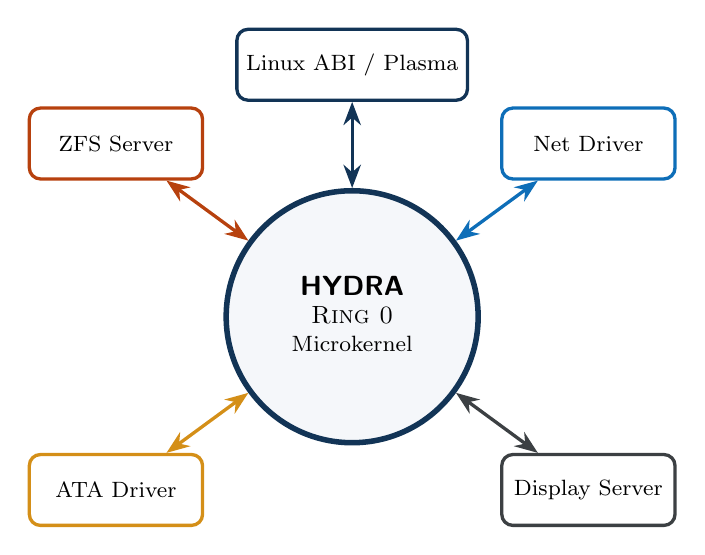
\begin{tikzpicture}
        % Stylized multi-headed hydra microkernel symbol
        \node[circle, draw=hydrablue, line width=2pt, fill=hydralight, minimum size=3.2cm] (core) at (0,0) {
            \begin{tabular}{c}
                \textbf{\sffamily HYDRA}\\[-2pt]
                \small\textsc{Ring 0}\\[-2pt]
                \footnotesize Microkernel
            \end{tabular}
        };
        
        \node[rectangle, rounded corners, draw=rustred, fill=white, line width=1.2pt, minimum width=2.2cm, minimum height=0.9cm] (zfs) at (-3, 2.2) {\footnotesize ZFS Server};
        \node[rectangle, rounded corners, draw=rustkeyword, fill=white, line width=1.2pt, minimum width=2.2cm, minimum height=0.9cm] (net) at (3, 2.2) {\footnotesize Net Driver};
        \node[rectangle, rounded corners, draw=hydragold, fill=white, line width=1.2pt, minimum width=2.2cm, minimum height=0.9cm] (ata) at (-3, -2.2) {\footnotesize ATA Driver};
        \node[rectangle, rounded corners, draw=hydragray, fill=white, line width=1.2pt, minimum width=2.2cm, minimum height=0.9cm] (disp) at (3, -2.2) {\footnotesize Display Server};
        \node[rectangle, rounded corners, draw=hydrablue, fill=white, line width=1.2pt, minimum width=2.6cm, minimum height=0.9cm] (posix) at (0, 3.2) {\footnotesize Linux ABI / Plasma};

        \draw[<->, >=Stealth, line width=1.2pt, rustred] (core) -- (zfs);
        \draw[<->, >=Stealth, line width=1.2pt, rustkeyword] (core) -- (net);
        \draw[<->, >=Stealth, line width=1.2pt, hydragold] (core) -- (ata);
        \draw[<->, >=Stealth, line width=1.2pt, hydragray] (core) -- (disp);
        \draw[<->, >=Stealth, line width=1.2pt, hydrablue] (core) -- (posix);
    \end{tikzpicture}
    
    \vfill
    
    {\large\sffamily Inspired by the classic works of \textbf{Andrew S. Tanenbaum}}\\[1.0cm]
    
    \textsf{\today}
\end{center}
\end{titlepage}


\thispagestyle{empty}
\vspace*{7cm}
\begin{center}
    \itshape
    Dedicated to Andrew S. Tanenbaum,\\
    whose pioneering work on MINIX and pedagogical mastery\\
    taught generations of computer scientists that an operating system\\
    can be clean, modular, reliable, and understood in its entirety.\\[1.5cm]
    And to the systems programmers striving to build\\
    a crash-resilient, memory-safe future.
\end{center}
\vfill

\chapter*{Preface}
\addcontentsline{toc}{chapter}{Preface}

In 1987, Andrew S. Tanenbaum published \textit{Operating Systems: Design and Implementation}. Accompanied by MINIX, a teaching operating system written in C for the original IBM PC, the book fundamentally altered computer science education. For the first time, students were not forced to study operating systems purely as abstract mathematical models of queuing networks, nor were they overwhelmed by hundreds of thousands of lines of convoluted industrial code. Instead, they could read a real, running operating system from beginning to end, study every system call, and understand how hardware transitions into software.

However, the computing landscape has transformed radically since the late 1980s:
\begin{enumerate}
    \item \textbf{Architectural Modernization:} The 16-bit real-mode x86 processors of MINIX~1 and 32-bit protected-mode x86 of MINIX~3 have been superseded by 64-bit multi-core architectures (x86\_64 Long Mode), UEFI firmware, Advanced Programmable Interrupt Controllers (APIC), PCI Express, and high-performance direct memory access (DMA).
    \item \textbf{Language Safety:} C remains ubiquitous, yet forty years of empirical evidence shows that over 70\% of critical operating system vulnerabilities stem from memory-safety errors: buffer overflows, use-after-free, double frees, and data races. The advent of \textbf{Rust} proves that bare-metal performance and zero-cost abstractions can coexist with strict, compiler-enforced memory safety and thread safety.
    \item \textbf{Storage Demands:} Classic file systems (like the MINIX V1/V2 file system or original UNIX FFS) lack data integrity guarantees. Modern production systems demand transactional, Copy-on-Write (CoW) enterprise storage pools with cryptographic Merkle tree verification, such as \textbf{OpenZFS}.
    \item \textbf{Application Compatibility:} A pure microkernel operating system with an esoteric API often languishes in isolation because porting modern software is prohibitively expensive. To be genuinely useful, a modern microkernel must be capable of hosting modern userland workloads—including dynamic linkers, Wayland display servers, desktop environments (KDE Plasma), and full web browsers (Brave, Chromium)—without compromising its core isolation principles.
\end{enumerate}

\section*{What is Hydra?}

\textbf{Hydra} is a from-scratch, modern, capability-oriented microkernel operating system written in Rust for the x86\_64 architecture. It borrows its philosophical foundation from Tanenbaum's MINIX: keep the Ring~0 privileged supervisor as small and verifiable as possible, while pushing device drivers, storage engines, network stacks, and display servers out into isolated Ring~3 user-space processes.

At the same time, Hydra introduces several major advancements:
\begin{itemize}
    \item \textbf{Pure Rust Microkernel Core:} The Ring~0 kernel is built with safe Rust abstractions wherever possible, isolating unsafe assembly instructions (like context switching and CR3 page table manipulations) behind bulletproof, type-checked boundaries.
    \item \textbf{Enterprise OpenZFS Storage Engine:} Hydra incorporates a native OpenZFS implementation directly into its storage hierarchy, featuring pooled storage (\texttt{hydrapool}), 64-bit object sets (dnodes), Copy-on-Write transactions, and Fletcher-4 checksumming.
    \item \textbf{Isolated Ring~3 Drivers:} Hardware device drivers (ATA/IDE bus-master DMA, Intel 82540EM Gigabit NIC, and graphics display servers) run as distinct Ring~3 processes communicating through synchronous IPC endpoints.
    \item \textbf{Linux Binary Compatibility Subsystem:} Hydra provides an in-kernel Linux ABI layer that intercepts x86\_64 \texttt{syscall} invocations, implements POSIX process and virtual filesystem semantics, and runs unmodified upstream Linux binaries—from GNU coreutils and Python to the SDDM display manager, KWin Wayland compositor, and KDE Plasma 6.
\end{itemize}

\section*{Structure of the Book}

Following the pedagogical tradition of Tanenbaum, this textbook is structured to take you from foundational principles to concrete, line-by-line implementation:

\begin{itemize}
    \item \textbf{Part I: Foundations \& Microkernel Architecture} (Chapters 1--3) explores the philosophy of operating systems, microkernel versus monolithic designs, x86\_64 bootstrap, preemptive process scheduling, thread control blocks, IPC rendezvous mechanics, and 4-level PML4 virtual memory management.
    \item \textbf{Part II: Storage, I/O \& Networking} (Chapters 4--6) examines the design of modern file systems with a complete dissection of Hydra's OpenZFS pool and transaction subsystem, followed by driver isolation principles, bus-master DMA, and the network protocol pipeline.
    \item \textbf{Part III: Subsystems, Compatibility \& Security} (Chapters 7--9) covers the Linux binary compatibility layer, dynamic ELF loading, the Wayland graphics pipeline, capability-based security, Rust-enforced guarantees, and an annotated walkthrough of the entire Hydra codebase.
    \item \textbf{Appendices} provide practical guides for compiling Hydra with Cargo, setting up bootable UEFI media in VirtualBox and QEMU, and a complete system call and hardware reference.
\end{itemize}

This book is intended for undergraduate and graduate computer science students, operating system developers, embedded systems engineers, and curious Rust enthusiasts who want to understand how a modern computer system really works from the hardware up.



\tableofcontents
\listoffigures
\listoftables

% ------------------------------------------------------------------------------
% Mainmatter
% ------------------------------------------------------------------------------
\mainmatter

\part{Foundations \& Microkernel Architecture}
\chapter{Introduction to Operating Systems \& Hydra Architecture}
\label{chap:introduction}

An operating system is the foundational software layer that stands between raw computer hardware and the application programs that perform meaningful work for users. Without an operating system, every programmer would be forced to write custom machine code to interact directly with motherboard chipsets, program disk controller registers, decode network packets from serial hardware, and handle interrupt dispatching manually.

As Andrew S. Tanenbaum famously observed in \textit{Operating Systems: Design and Implementation}~\cite{tanenbaum2006operating}, an operating system performs two primary, complementary roles:
\begin{enumerate}
    \item \textbf{An Extended Machine (Top-Down View):} It provides convenient, high-level abstractions—such as processes, threads, virtual address spaces, files, sockets, and graphical surfaces—hiding the idiosyncratic and often grotesque complexity of the physical hardware.
    \item \textbf{A Resource Manager (Bottom-Up View):} It multiplexes the CPU cores, physical memory frames, I/O ports, and network interfaces among competing processes, enforcing isolation, fairness, and security.
\end{enumerate}

In this opening chapter, we re-evaluate these fundamental concepts through the lens of modern computing hardware and introduce the architectural philosophy of \textbf{Hydra}.

% ==============================================================================
\section{Microkernels vs. Monolithic Systems: The Modern Paradigm}
\label{sec:micro_vs_mono}
% ==============================================================================

For decades, the operating systems community engaged in intense debate regarding the ideal internal structure of an operating system kernel. In a traditional \textbf{monolithic operating system} (such as Linux, FreeBSD, or Windows NT), virtually every major subsystem executes within a single, unified address space in the processor's most privileged execution mode (\textsc{Ring~0} on x86\_64).

\begin{figure}[htbp]
\centering
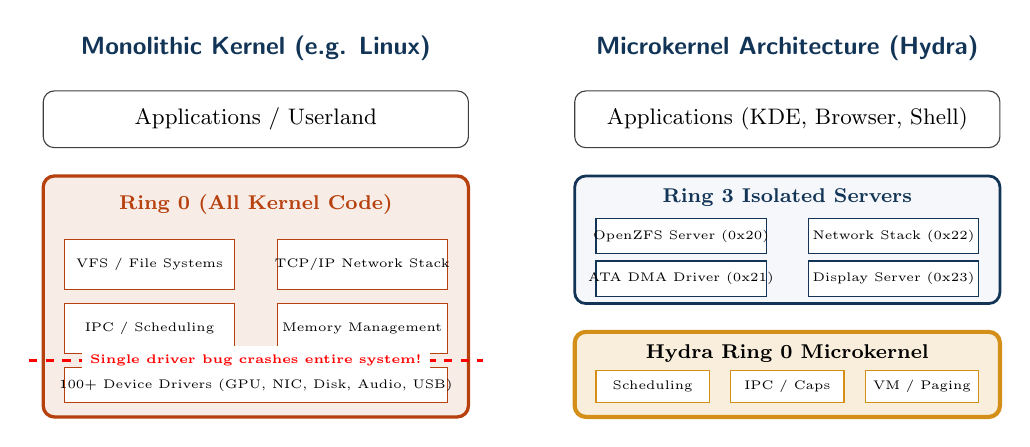
\begin{tikzpicture}[scale=0.9, every node/.style={transform shape}]
    % Monolithic Kernel
    \begin{scope}[shift={(0,0)}]
        \node[font=\bfseries\sffamily, hydrablue] at (3, 5.2) {Monolithic Kernel (e.g. Linux)};
        
        \draw[fill=white, draw=hydragray, rounded corners] (0, 3.8) rectangle (6, 4.6);
        \node at (3, 4.2) {\small Applications / Userland};
        
        \draw[fill=rustred!10, draw=rustred, line width=1.2pt, rounded corners] (0, 0) rectangle (6, 3.4);
        \node[font=\bfseries\footnotesize\color{rustred}] at (3, 3.0) {Ring 0 (All Kernel Code)};
        
        \draw[fill=white, draw=rustred] (0.3, 1.8) rectangle (2.7, 2.5) node[pos=0.5] {\tiny VFS / File Systems};
        \draw[fill=white, draw=rustred] (3.3, 1.8) rectangle (5.7, 2.5) node[pos=0.5] {\tiny TCP/IP Network Stack};
        \draw[fill=white, draw=rustred] (0.3, 0.9) rectangle (2.7, 1.6) node[pos=0.5] {\tiny IPC / Scheduling};
        \draw[fill=white, draw=rustred] (3.3, 0.9) rectangle (5.7, 1.6) node[pos=0.5] {\tiny Memory Management};
        \draw[fill=white, draw=rustred] (0.3, 0.2) rectangle (5.7, 0.7) node[pos=0.5] {\tiny 100+ Device Drivers (GPU, NIC, Disk, Audio, USB)};
        
        \draw[dashed, red, line width=1pt] (-0.2, 0.8) -- (6.2, 0.8);
        \node[red, font=\tiny\bfseries, fill=white] at (3, 0.8) {Single driver bug crashes entire system!};
    \end{scope}

    % Microkernel Architecture
    \begin{scope}[shift={(7.5,0)}]
        \node[font=\bfseries\sffamily, hydrablue] at (3, 5.2) {Microkernel Architecture (Hydra)};
        
        \draw[fill=white, draw=hydragray, rounded corners] (0, 3.8) rectangle (6, 4.6);
        \node at (3, 4.2) {\small Applications (KDE, Browser, Shell)};
        
        % Ring 3 Servers
        \draw[fill=hydralight, draw=hydrablue, line width=1pt, rounded corners] (0, 1.6) rectangle (6, 3.4);
        \node[font=\bfseries\footnotesize\color{hydrablue}] at (3, 3.1) {Ring 3 Isolated Servers};
        
        \draw[fill=white, draw=hydrablue] (0.3, 2.3) rectangle (2.7, 2.8) node[pos=0.5] {\tiny OpenZFS Server (0x20)};
        \draw[fill=white, draw=hydrablue] (3.3, 2.3) rectangle (5.7, 2.8) node[pos=0.5] {\tiny Network Stack (0x22)};
        \draw[fill=white, draw=hydrablue] (0.3, 1.7) rectangle (2.7, 2.2) node[pos=0.5] {\tiny ATA DMA Driver (0x21)};
        \draw[fill=white, draw=hydrablue] (3.3, 1.7) rectangle (5.7, 2.2) node[pos=0.5] {\tiny Display Server (0x23)};
        
        % Ring 0 Microkernel
        \draw[fill=hydragold!15, draw=hydragold, line width=1.5pt, rounded corners] (0, 0) rectangle (6, 1.2);
        \node[font=\bfseries\footnotesize\color{black}] at (3, 0.9) {Hydra Ring 0 Microkernel};
        \draw[fill=white, draw=hydragold] (0.3, 0.2) rectangle (1.9, 0.65) node[pos=0.5] {\tiny Scheduling};
        \draw[fill=white, draw=hydragold] (2.2, 0.2) rectangle (3.8, 0.65) node[pos=0.5] {\tiny IPC / Caps};
        \draw[fill=white, draw=hydragold] (4.1, 0.2) rectangle (5.7, 0.65) node[pos=0.5] {\tiny VM / Paging};
    \end{scope}
\end{tikzpicture}
\caption{Comparison between Monolithic Kernels and Hydra's Microkernel Architecture.}
\label{fig:mono_vs_micro}
\end{figure}

The consequence of the monolithic approach is severe:
\begin{itemize}
    \item \textbf{Catastrophic Blast Radius:} Device drivers account for over 70\% of a modern monolithic kernel's codebase. A null pointer dereference, buffer overrun, or infinite loop inside a single graphics driver or USB controller brings down the entire operating system, provoking a kernel panic or Blue Screen of Death.
    \item \textbf{Absence of Principle of Least Privilege:} A network driver handling incoming Ethernet frames has unrestricted permission to read or overwrite the page tables of every user process, disk encryption keys, or the physical frame allocator.
\end{itemize}

\begin{designprinciple}[Liedtke's Postulate]
A concept is tolerated inside the microkernel \textbf{only} if moving it outside the kernel, i.e., permitting competing implementations, would prevent the implementation of the system's required functionality~\cite{liedtke1995microkernel}.
\end{designprinciple}

Hydra adheres strictly to this mandate. The Ring~0 core of Hydra is restricted to:
\begin{enumerate}
    \item \textbf{Thread Management and Preemptive Scheduling:} Creating threads, restoring CPU registers, and switching execution contexts.
    \item \textbf{Interprocess Communication (IPC):} Providing synchronous message rendezvous and capability tokens between endpoints.
    \item \textbf{Virtual Memory Primitives:} Managing 4-level x86\_64 PML4 page tables and mapping physical frames to virtual addresses.
    \item \textbf{Hardware Interrupt Dispatching:} Remapping hardware interrupt requests (IRQs) into lightweight IPC notification signals.
\end{enumerate}

Everything else—the OpenZFS file system engine, the ATA DMA disk controller driver, the Intel 82540EM network driver, the DRM/KMS display server, and the D-Bus session manager—runs exclusively as isolated Ring~3 user-space processes. If the network driver crashes due to a malformed packet, it simply terminates; the microkernel detects its exit, restarts the driver server process, and the rest of the operating system continues executing uninterrupted.

% ==============================================================================
\section{The Language Dimension: Why Rust?}
\label{sec:why_rust}
% ==============================================================================

When Andrew Tanenbaum created MINIX, C was the natural choice. It offered unmatched access to hardware memory addresses and direct mapping to CPU assembly instructions. However, C lacks any compiler-enforced guarantees regarding memory safety or thread safety.

In Hydra, the microkernel and all core servers are authored in \textbf{Rust}. Rust provides three crucial properties for modern systems programming:
\begin{itemize}
    \item \textbf{Compile-Time Ownership and Borrowing:} The compiler enforces strict aliasing rules: you may have any number of immutable references (\texttt{\&T}) or exactly one mutable reference (\texttt{\&mut T}), but never both simultaneously. This eliminates data races and memory corruption at compile time.
    \item \textbf{Zero-Cost Abstractions:} Higher-level abstractions—such as iterators, pattern matching, closures, strong typing, and smart pointers—compile into machine code that is as fast or faster than hand-written C.
    \item \textbf{Explicit \texttt{unsafe} Boundaries:} In an operating system kernel, interacting with physical hardware necessarily requires dereferencing raw pointers, manipulating control registers (\texttt{CR0}, \texttt{CR3}, \texttt{CR4}), and loading segment registers. In Rust, these operations are strictly sequestered inside clearly marked \texttt{unsafe} blocks. Over 95\% of Hydra's codebase is verified safe by the compiler.
\end{itemize}

% ==============================================================================
\section{Hydra System Architecture Overview}
\label{sec:hydra_overview}
% ==============================================================================

Hydra boots via modern 64-bit UEFI firmware. Upon acquiring control, the Hydra boot loader performs the definitive hardware takeover:
\begin{enumerate}
    \item Captures the UEFI memory map and calls \texttt{ExitBootServices}, terminating firmware interference.
    \item Initializes the x86\_64 Global Descriptor Table (GDT) and Task State Segment (TSS) with Ring~0 and Ring~3 code/data selectors.
    \item Loads an autonomous 4-level PML4 page table root and reprograms the MSRs for hardware \texttt{SYSCALL}/\texttt{SYSRET} execution.
    \item Initializes the OpenZFS storage pool (\texttt{hydrapool}) and mounts root datasets.
    \item Spawns the Ring~3 isolated service hierarchy:
    \begin{itemize}
        \item \textbf{Process 2 (Endpoint 0x21):} \texttt{ata\_driver} (Bus-Master DMA Disk Server)
        \item \textbf{Process 3 (Endpoint 0x20):} \texttt{zfs\_server} (OpenZFS File System Server)
        \item \textbf{Process 4 (Endpoint 0x22):} \texttt{net\_driver} (Intel 82540EM Gigabit NIC Server)
        \item \textbf{Process 5 (Endpoint 0x23):} \texttt{display\_server} (DRM/KMS Graphics Server)
    \end{itemize}
    \item Mounts the Linux compatibility environment and launches the graphical userland (SDDM, KWin Wayland, and KDE Plasma 6).
\end{enumerate}

\begin{tanenbaumnote}[The Hydra Boot Log]
When Hydra initializes on hardware or VirtualBox, the microkernel console logs each milestone:
\begin{verbatim}
[*] Step 6: Initializing Devices & Reading the Boot Volume...
[+] Boot volume: 43 files staged for the pool
[*] Step 7: Initializing Multitasking Scheduler...
[+] OpenZFS: Imported pool 'hydrapool' (16384 MiB, TXG #52688)
[supervisor] started 'ata_driver' (process 2, endpoint 0x21)
[supervisor] started 'zfs_server' (process 3, endpoint 0x20)
[supervisor] started 'net_driver' (process 4, endpoint 0x22)
[supervisor] started 'display_server' (process 5, endpoint 0x23)
[*] Starting the login screen (SDDM)...
\end{verbatim}
Notice that the entire storage, network, and display stacks are initialized as Ring~3 user-space servers managed by the microkernel supervisor.
\end{tanenbaumnote}

% ==============================================================================
\section{Summary and Outline of the Book}
\label{sec:outline}
% ==============================================================================

Modern operating systems design requires synthesizing theoretical principles with real-world engineering constraints. Over the following chapters, we dissect every layer of Hydra:
\begin{itemize}
    \item Chapter~\ref{chap:processes} examines processes, threads, context switching, and interprocess communication.
    \item Chapter~\ref{chap:memory} explores virtual memory, 4-level paging, frame allocation, and page fault handling.
    \item Chapter~\ref{chap:zfs} provides a deep technical analysis of Hydra's OpenZFS Copy-on-Write file system implementation.
    \item Chapter~\ref{chap:io} covers device drivers, hardware interrupts, bus-master DMA, and driver isolation.
    \item Chapter~\ref{chap:networking} covers the zero-copy network architecture and TCP/IP stack.
    \item Chapter~\ref{chap:linux_compat} explains how Hydra hosts full unmodified Linux desktop environments.
    \item Chapter~\ref{chap:security} analyzes capability-based security and memory safety.
    \item Chapter~\ref{chap:source_tour} presents an annotated source code tour of the entire operating system.
\end{itemize}


\chapter{Processes, Threads, and Scheduling}
\label{chap:processes}

In any multitasking operating system, the most central abstraction is the \textbf{process}. A process is simply an executing program along with all the state required to run it: its virtual address space, CPU register values, thread stacks, file descriptor tables, IPC channels, and security credentials.

Tanenbaum famously compared a computer running multiple processes to a busy chef baking cakes~\cite{tanenbaum2006operating}: the chef (the CPU) switches rapidly between distinct recipes (the programs) and their respective bowls of ingredients (the address spaces). To the outside observer, multiple cakes appear to be rising simultaneously.

In this chapter, we explore how modern operating systems structure processes and threads, examine the mathematical and algorithmic foundations of CPU scheduling, dive into mutual exclusion and synchronization primitives (from hardware atomic instructions to Linux-compatible futexes), and dissect the implementation of Hydra's preemptive scheduler and context switch engine.

% ==============================================================================
\section{The Process Model}
\label{sec:process_model}
% ==============================================================================

In modern operating systems, all runnable software is organized into one or more sequential processes. A process is an independent execution entity consisting of:
\begin{enumerate}
    \item \textbf{A Private Virtual Address Space:} Mapped via hardware page tables, ensuring that the process can read and write only its own memory cells.
    \item \textbf{A Thread of Execution:} A sequential stream of instructions guided by a Program Counter (the \texttt{RIP} register on x86\_64) and executed in the context of processor registers and a stack.
    \item \textbf{Kernel-Managed Resources:} File descriptor tables, capability rights tokens, signal masks, parent-child relationships, and memory-mapped files.
\end{enumerate}

\subsection{Process Creation and Lifecycle}
Operating systems create processes in four primary situations:
\begin{enumerate}
    \item \textbf{System Initialization:} When the kernel boots, it initializes hardware subsystems and creates root processes (such as the Hydra shell, the idle task, and the supervisor).
    \item \textbf{Execution of a Process Creation System Call:} An actively running process invokes a system call (such as \texttt{fork()}, \texttt{clone()}, or \texttt{posix\_spawn()}) to launch a subsidiary process.
    \item \textbf{User Request:} An interactive user types a command into the shell or double-clicks an application icon in a graphical desktop environment (e.g., KDE Plasma).
    \item \textbf{Batch Job Initiation:} A job scheduler (such as cron or a compute cluster manager) activates a queued batch job.
\end{enumerate}

In UNIX and modern POSIX-compliant systems, process creation is classically split into two complementary system calls:
\begin{itemize}
    \item \texttt{fork()}: Creates an exact duplicate of the calling process, including an identical copy of the virtual address space (implemented with high efficiency using Copy-on-Write page table manipulation).
    \item \texttt{execve()}: Replaces the calling process's current memory image, code segment, and heap with a new binary executable file read from disk (such as an ELF binary), resetting registers and commencing execution at the new entry point.
\end{itemize}

\subsection{Process Termination}
A process terminates under one of four conditions:
\begin{enumerate}
    \item \textbf{Normal Exit (Voluntary):} The process completes its task and invokes \texttt{exit(0)} (system call \texttt{sys\_exit}).
    \item \textbf{Error Exit (Voluntary):} The process encounters a fatal logic error (e.g., a compiler fails to open an input source file) and invokes \texttt{exit(status)} with a non-zero exit code.
    \item \textbf{Fatal Error (Involuntary):} The process triggers an unhandled CPU exception (e.g., dividing by zero, dereferencing an unmapped memory address triggering a Page Fault \texttt{\#PF}, or executing an illegal instruction triggering an Invalid Opcode \texttt{\#UD}). The kernel terminates the process, optionally generating a core dump file.
    \item \textbf{Killed by Another Process (Involuntary):} Another authorized process or the operating system sends a terminating signal (e.g., \texttt{SIGKILL} or \texttt{SIGTERM}) via the \texttt{kill()} system call.
\end{enumerate}

\subsection{Process Hierarchies and State Transitions}
In Hydra, as in UNIX, processes are organized into a strict hierarchical tree rooted at the initial supervisor process (\texttt{PID~1}). When a parent process spawns a child, the parent remains responsible for reaping the child when it terminates.

A process transitions through distinct states during its lifespan, as illustrated in Figure~\ref{fig:process_states}:
\begin{itemize}
    \item \textbf{Running:} The process is actively executing machine instructions on a CPU core.
    \item \textbf{Ready:} The process is fully prepared to execute, but is temporarily suspended waiting for the scheduler to allocate it a CPU time slice.
    \item \textbf{Blocked:} The process cannot execute because it is waiting for an external event (e.g., disk I/O completion, an incoming network packet, or a synchronous IPC rendezvous). Even if a CPU core were free, the process cannot run.
    \item \textbf{Sleeping:} A specialized blocked state in which the process is paused until a target timer tick is reached (e.g., via \texttt{nanosleep()}).
    \item \textbf{Dead / Zombie:} The process has terminated execution. Its memory and file descriptors have been released, but its \texttt{TaskControlBlock} remains in the process table so that its parent can inspect its final exit status code via \texttt{waitpid()}. Once reaped, the entry is deleted.
\end{itemize}

\begin{figure}[htbp]
\centering
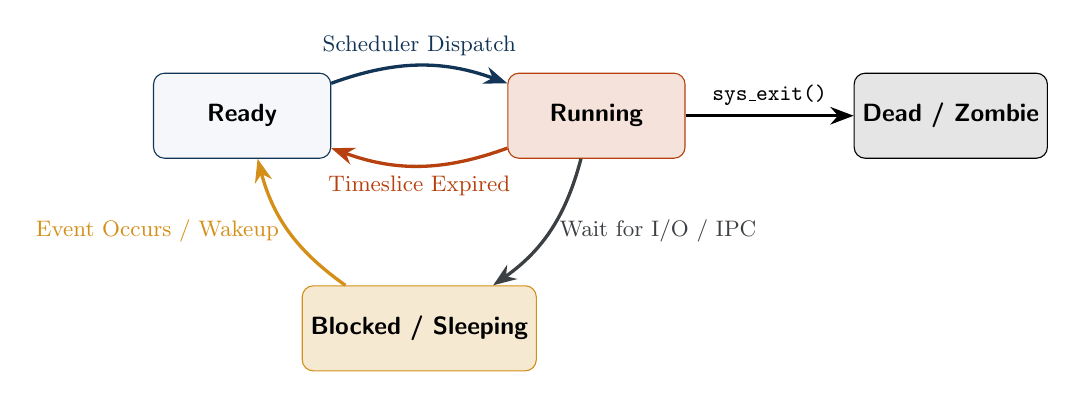
\begin{tikzpicture}[scale=0.9, every node/.style={transform shape}]
    \node[draw=hydrablue, fill=hydralight, rounded corners, minimum width=2.5cm, minimum height=1.2cm, font=\bfseries\sffamily] (ready) at (0, 0) {Ready};
    \node[draw=rustred, fill=rustred!15, rounded corners, minimum width=2.5cm, minimum height=1.2cm, font=\bfseries\sffamily] (running) at (5, 0) {Running};
    \node[draw=hydragold, fill=hydragold!20, rounded corners, minimum width=2.5cm, minimum height=1.2cm, font=\bfseries\sffamily] (blocked) at (2.5, -3) {Blocked / Sleeping};
    \node[draw=black, fill=gray!20, rounded corners, minimum width=2.5cm, minimum height=1.2cm, font=\bfseries\sffamily] (dead) at (10, 0) {Dead / Zombie};

    \draw[->, >=Stealth, line width=1.2pt, hydrablue] (ready) to[bend left=20] node[above] {\small Scheduler Dispatch} (running);
    \draw[->, >=Stealth, line width=1.2pt, rustred] (running) to[bend left=20] node[below] {\small Timeslice Expired} (ready);
    \draw[->, >=Stealth, line width=1.2pt, hydragray] (running) to[bend left=20] node[right] {\small Wait for I/O / IPC} (blocked);
    \draw[->, >=Stealth, line width=1.2pt, hydragold] (blocked) to[bend left=20] node[left] {\small Event Occurs / Wakeup} (ready);
    \draw[->, >=Stealth, line width=1.2pt, black] (running) -- node[above] {\small \texttt{sys\_exit()}} (dead);
\end{tikzpicture}
\caption{The Process State Transition Diagram in Hydra.}
\label{fig:process_states}
\end{figure}

% ==============================================================================
\section{The Thread Model and Multithreading}
\label{sec:thread_model}
% ==============================================================================

In traditional operating systems, each process possessed a single thread of control. However, modern software systems perform multiple concurrent activities within the same application:
\begin{itemize}
    \item A web browser must concurrently render HTML elements, execute JavaScript animations, stream video, and download incoming TCP packets over multiple connections.
    \item A database server must service hundreds of concurrent client queries while background threads flush write-ahead transaction logs to disk.
\end{itemize}

\subsection{Threads versus Processes}
A \textbf{thread} (or lightweight process) is an independent execution context that shares an address space and open file descriptors with other threads in the same process:

\begin{table}[htbp]
\centering
\small
\begin{tabular}{ll}
\hline
\textbf{Per-Process Items (Shared by all Threads)} & \textbf{Per-Thread Items (Private to each Thread)} \\
\hline
Virtual Address Space (PML4 page tables) & Program Counter (\texttt{RIP}) \\
Executable Machine Code & CPU Register Set (\texttt{RAX}, \texttt{RBX}, etc.) \\
Global Variables and Static Data & Execution Stack (Stack Pointer \texttt{RSP}) \\
Heap Allocations & Thread-Local Storage (TLS, via \texttt{FS\_BASE}) \\
Open File Descriptor Table & Scheduling Priority and State \\
IPC Capability Descriptors & Saved FPU / SSE / AVX Context \\
Signal Handlers and Process ID (\texttt{PID}) & Signal Mask and Thread ID (\texttt{TID}) \\
\hline
\end{tabular}
\caption{Partitioning of Shared Process State vs. Private Thread State.}
\label{tab:thread_state}
\end{table}

Because threads share the same address space, context switching between two threads in the same process is significantly faster than switching between different processes: \textbf{the CPU's \texttt{CR3} register does not need to be reloaded}, preserving the Translation Lookaside Buffer (TLB) cache and avoiding expensive virtual memory pipeline flushes.

\subsection{User-Level Threads versus Kernel-Level Threads}
Operating system architectures implement multithreading via two distinct models:
\begin{enumerate}
    \item \textbf{User-Level Threads (1:N Model):} The kernel is unaware of the existence of multiple threads; it manages only single-threaded processes. A user-space runtime library (such as a coroutine or green thread package) implements thread creation, switching, and scheduling entirely in user space.
    \begin{itemize}
        \item \textit{Advantage:} Thread creation and context switching require zero kernel system calls; switching threads takes only tens of nanoseconds.
        \item \textit{Fatal Flaw:} If one user thread executes a blocking system call (e.g., reading from a disk or socket), the entire process and all other user threads are blocked by the kernel. Furthermore, user threads cannot take advantage of multiple physical CPU cores simultaneously.
    \end{itemize}
    \item \textbf{Kernel-Level Threads (1:1 Model):} The kernel maintains a dedicated \texttt{TaskControlBlock} for every thread. The kernel scheduler directly dispatches threads onto available CPU cores.
    \begin{itemize}
        \item \textit{Advantage:} If thread A blocks on an I/O operation, the kernel independently schedules thread B. Multiple threads run truly concurrently on multiple CPU cores.
        \item \textit{Trade-off:} Context switching between threads requires crossing into the kernel, incurring trap overhead.
    \end{itemize}
\end{enumerate}

Hydra implements the **1:1 Kernel-Level Thread Model**, unifying threads and processes under the extensible \texttt{Task} structure.

% ==============================================================================
\section{Interprocess Communication and Synchronization}
\label{sec:ipc_sync}
% ==============================================================================

Whenever multiple processes or threads execute concurrently, they must coordinate their actions and share data. However, unconstrained concurrent access to shared resources introduces one of the most pernicious bugs in computer science: the \textbf{race condition}.

\subsection{Race Conditions and Critical Regions}
A \textbf{race condition} occurs when two or more threads read and write shared data, and the final outcome depends on the exact, unpredictable order in which instructions are interleaved by the CPU scheduler.

\begin{tanenbaumnote}[The Classic Spooler Directory Race]
Consider a print spooler directory. Two processes, $P_1$ and $P_2$, wish to queue print jobs. A shared global variable, \texttt{out}, stores the index of the next free slot (e.g., slot 7).
\begin{enumerate}
    \item Process $P_1$ reads \texttt{out} and observes that slot 7 is free.
    \item Before $P_1$ can write its filename into slot 7, a timer interrupt occurs. The scheduler preempts $P_1$ and switches to $P_2$.
    \item Process $P_2$ reads \texttt{out}, also observes slot 7, writes its filename into slot 7, increments \texttt{out} to 8, and yields.
    \item The scheduler resumes $P_1$. Process $P_1$ believes slot 7 is still its allocated slot, overwrites $P_2$'s filename in slot 7, and increments \texttt{out} to 8!
\end{enumerate}
Process $P_2$'s print job is completely erased and lost forever.
\end{tanenbaumnote}

To prevent race conditions, any segment of code that accesses shared memory must be treated as a \textbf{critical region}. To achieve correct concurrent execution, four conditions must be met:
\begin{enumerate}
    \item \textbf{Mutual Exclusion:} No two processes may be simultaneously inside their critical regions accessing the same resource.
    \item \textbf{No Assumptions about Hardware Speed:} No assumptions may be made about the speeds or number of CPU cores.
    \item \textbf{No Starvation (Progress):} No process running outside its critical region may block other processes from entering.
    \item \textbf{Bounded Waiting:} No process should have to wait indefinitely to enter its critical region.
\end{enumerate}

\subsection{Hardware Support for Mutual Exclusion}
Early software algorithms (such as Peterson's Algorithm) demonstrated that mutual exclusion was theoretically achievable on single-core uniprocessors using plain loads and stores. However, modern out-of-order, multi-core superscalar processors aggressively reorder memory reads and writes, invalidating software-only algorithms unless explicit memory barrier instructions are used.

Modern hardware provides atomic Read-Modify-Write instructions:
\begin{itemize}
    \item \textbf{Test-and-Set Lock (TSL):} Reads a memory location into a register and writes a non-zero value to the memory word in an indivisible hardware operation.
    \item \textbf{Compare-and-Swap (CAS / \texttt{CMPXCHG}):} Compares the contents of a memory location to an expected value; if equal, it updates the location to a new value. On x86\_64, prefixing the instruction with the \texttt{lock} bus signal (\texttt{lock cmpxchg}) asserts hardware cache coherency protocols (MESI/MOESI), guaranteeing atomic execution across all CPU cores.
\end{itemize}

In Hydra, low-level spinlocks are built directly upon atomic CAS operations:
\begin{lstlisting}[language=Rust, caption={Atomic Spinlock Primitive in Hydra (\texttt{src/sync/mutex.rs})}]
use core::sync::atomic::{AtomicBool, Ordering};

pub struct SpinLock {
    locked: AtomicBool,
}

impl SpinLock {
    pub const fn new() -> Self {
        Self { locked: AtomicBool::new(false) }
    }

    pub fn lock(&self) {
        while self.locked.compare_exchange_weak(
            false,
            true,
            Ordering::Acquire,
            Ordering::Relaxed
        ).is_err() {
            // Hint to CPU execution pipeline that we are spin-waiting
            core::hint::spin_loop();
        }
    }

    pub fn unlock(&self) {
        self.locked.store(false, Ordering::Release);
    }
}
\end{lstlisting}

\subsection{Semaphores, Mutexes, and Futexes}
While spinlocks are ideal for short, microsecond critical sections inside the Ring~0 kernel, they are disastrous in user space: a user-space thread spinning on a locked variable wastes CPU cycles that could be utilized by productive worker threads.

\begin{enumerate}
    \item \textbf{Counting Semaphores (Dijkstra):} A semaphore $S$ is an integer variable accessed only through two atomic operations:
    \begin{itemize}
        \item \texttt{down(S)} (or \texttt{P(S)}): Decrements $S$. If $S < 0$, the calling thread is suspended on the semaphore's wait queue.
        \item \texttt{up(S)} (or \texttt{V(S)}): Increments $S$. If $S \le 0$, one blocked thread is removed from the wait queue and awakened.
    \end{itemize}
    \item \textbf{Mutexes (Mutual Exclusion Locks):} A binary semaphore initialized to 1, with the strict requirement that only the thread that locked the mutex may unlock it.
    \item \textbf{Futexes (Fast User-Space Mutexes):} In traditional UNIX, locking a mutex always required a system call to the kernel. A \textbf{futex} optimizes the common, uncontended case:
    \begin{itemize}
        \item If the lock is free, the user thread acquires it via a single atomic \texttt{lock cmpxchg} instruction in user space, with \textbf{zero system call overhead}.
        \item Only if contention is detected does the thread invoke the \texttt{sys\_futex(addr, FUTEX\_WAIT, val)} system call, asking the kernel to suspend it until another thread calls \texttt{FUTEX\_WAKE}.
    \end{itemize}
\end{enumerate}

Hydra provides a full implementation of the Linux \texttt{futex} ABI in \texttt{src/compat/linux/futex.rs}, enabling unmodified glibc, musl, and KDE Plasma synchronization primitives to execute with native speed.

% ==============================================================================
\section{Classical Synchronization Problems}
\label{sec:classical_problems}
% ==============================================================================

To test and illustrate concurrency mechanisms, computer scientists have formulated classic synchronization paradigms:

\subsection{The Producer-Consumer (Bounded Buffer) Problem}
Two processes share a fixed-size circular buffer of $N$ slots. The \textbf{producer} continuously generates data items and deposits them into the buffer; the \textbf{consumer} continuously removes items and processes them.
\begin{itemize}
    \item The producer must not attempt to deposit data if the buffer is completely full.
    \item The consumer must not attempt to extract data if the buffer is completely empty.
\end{itemize}

In Hydra, inter-thread channels solve this problem using two counting semaphores (\texttt{empty\_slots} initialized to $N$, and \texttt{full\_slots} initialized to 0) combined with a mutex protecting buffer insertion pointers.

\subsection{The Readers-Writers Problem}
A database or file structure is shared among multiple concurrent processes. Any number of \textbf{readers} may safely inspect the database simultaneously without interference. However, if a \textbf{writer} is updating the database, no other process (neither reader nor writer) may access the resource.
\begin{itemize}
    \item \textit{Reader Preference:} Readers are never forced to wait unless a writer is actively modifying the data. This risks \textbf{writer starvation}: a continuous stream of readers can delay a writer indefinitely.
    \item \textit{Writer Preference:} When a writer announces its intent to write, newly arriving readers are queued behind the writer, preventing starvation.
\end{itemize}

Hydra's VFS layer implements writer-priority Reader-Writer locks (\texttt{RwLock}) to ensure that metadata modifications to OpenZFS dnodes never suffer from starvation.

\subsection{The Dining Philosophers Problem}
Five philosophers sit around a circular table. In front of each is a bowl of noodles. Between each pair of adjacent philosophers lies a single fork (5 forks total). To eat, a philosopher must acquire \textit{both} their left and right forks.

If every philosopher simultaneously picks up their left fork, no right fork is available. Every philosopher holds one fork and waits indefinitely for the adjacent fork to be released: the system is in an unrecoverable state of \textbf{deadlock}.

Dijkstra's solution, implemented in operating systems resource allocation graphs, requires acquiring resources according to a global total ordering or testing fork availability atomically under a mutex.

% ==============================================================================
\section{The Hydra Task Control Block (TCB)}
\label{sec:hydra_tcb}
% ==============================================================================

In the Hydra microkernel, every process and thread is encapsulated by an instance of the canonical \texttt{Task} struct in \texttt{src/task/tcb.rs}.

\subsection{Detailed Architectural Layout}
The \texttt{Task} control block unifies CPU registers, privilege rings, memory maps, capability tables, and POSIX state into a single coherent record:

\begin{lstlisting}[language=Rust, caption={The Complete Task Control Block in Hydra (\texttt{src/task/tcb.rs})}]
pub struct Task {
    /// Unique 64-bit Task Identifier (PID / TID)
    pub id: TaskId,
    /// Parent process identifier (for POSIX process tree)
    pub parent_id: Option<TaskId>,
    /// Current execution state: Ready, Running, Blocked, Sleeping, Dead
    pub state: TaskState,
    /// Scheduling priority: Idle (0), Low (1), Normal (2), High (3), Realtime (4)
    pub priority: TaskPriority,
    /// Physical address of the task's Level-4 Page Map root (CR3)
    pub cr3: u64,
    /// Saved 64-bit general-purpose CPU register context
    pub registers: TaskRegisters,
    /// Base address of Thread-Local Storage (MSR IA32_FS_BASE)
    pub fs_base: u64,
    /// Base address of the task's dedicated kernel stack (64 KiB)
    pub stack_base: u64,
    pub stack_size: usize,
    /// Saved x87 FPU, MMX, and SSE/AVX register state (512 bytes)
    pub fpu_state: Box<FpuState>,
    /// Execution privilege mode (Ring 0 Kernel vs Ring 3 Userland)
    pub privilege: PrivilegeMode,
    /// ABI personality (Native Hydra vs Linux x86_64 ABI)
    pub personality: TaskPersonality,
    /// Capability table holding object reference rights
    pub capabilities: CapabilityTable,
    /// Remaining ticks in the current timeslice
    pub timeslice_remaining: u32,
    /// Starvation prevention counter
    pub starvation_ticks: u32,
    /// Total CPU runtime accumulated in timer ticks
    pub total_cpu_ticks: u64,
}
\end{lstlisting}

\subsection{Hardware Register Preservation (\texttt{TaskRegisters})}
The \texttt{TaskRegisters} structure mirrors the exact layout of the x86\_64 architectural register set:

\begin{lstlisting}[language=Rust, caption={x86\_64 Register Context (\texttt{src/task/tcb.rs})}]
#[derive(Debug, Clone, Copy)]
pub struct TaskRegisters {
    pub r15: u64, pub r14: u64, pub r13: u64, pub r12: u64,
    pub rbp: u64, pub rbx: u64, pub r11: u64, pub r10: u64,
    pub r9:  u64, pub r8:  u64, pub rdi: u64, pub rsi: u64,
    pub rdx: u64, pub rcx: u64, pub rax: u64,
    pub rip: u64,    // Instruction pointer
    pub cs:  u64,    // Code Segment (0x08 for Ring 0, 0x23 for Ring 3)
    pub rflags: u64, // CPU flags (Interrupt Flag IF, IO Privilege IOPL)
    pub rsp: u64,    // Stack pointer
    pub ss:  u64,    // Stack Segment (0x10 for Ring 0, 0x1B for Ring 3)
}
\end{lstlisting}

% ==============================================================================
\section{Context Switching on x86\_64: Hardware and Assembly}
\label{sec:context_switch_deep}
% ==============================================================================

A context switch is the physical mechanism by which the CPU halts execution of one thread and resumes execution of another. In Hydra, context switches occur either **preemptively** (driven by the 100~Hz PIT timer interrupt) or **cooperatively** (when a thread blocks on an IPC message or issues a yield interrupt \texttt{int 0x81}).

\subsection{The Anatomy of an Interrupt Context Switch}
When a timer interrupt fires, the x86\_64 processor executes an atomic transition from user mode to kernel mode:
\begin{enumerate}
    \item The CPU switches the stack pointer to the privileged Ring~0 stack defined in the Task State Segment (\texttt{TSS.RSP0}).
    \item The CPU automatically pushes five crucial registers onto the kernel stack in reverse order:
    \[
        \texttt{SS} \longrightarrow \texttt{RSP} \longrightarrow \texttt{RFLAGS} \longrightarrow \texttt{CS} \longrightarrow \texttt{RIP}
    \]
    \item The CPU loads the Interrupt Descriptor Table (IDT) entry for Vector~32 (IRQ~0) and jumps to the interrupt stub in \texttt{src/arch/idt.rs}.
    \item The Hydra assembly stub pushes all fifteen remaining general-purpose registers onto the stack, constructing a complete \texttt{ExceptionContext} frame.
\end{enumerate}

\subsection{The Assembly Context Switch Engine}
The core scheduler routine, \texttt{schedule()} in \texttt{src/task/scheduler.rs}, evaluates the task queue. If the currently running task has expired its timeslice, or if a higher-priority task has awakened, the scheduler copies the saved \texttt{ExceptionContext} from the stack into the outgoing task's \texttt{TaskRegisters}.

Next, the scheduler invokes the context-switch sequence:
\begin{enumerate}
    \item \textbf{FPU/SIMD State Preservation:} The x87/SSE/AVX state (including registers \texttt{XMM0} through \texttt{XMM15}) is saved via the \texttt{fxsave64} or \texttt{xsave} machine instruction into the outgoing task's \texttt{FpuState} buffer.
    \item \textbf{Thread-Local Storage (TLS) Update:} Modern x86\_64 compilers locate thread-local variables relative to the \texttt{FS} segment register. The kernel updates the \texttt{IA32\_FS\_BASE} Machine Specific Register (MSR \texttt{0xC000\_0100}) to the incoming task's \texttt{fs\_base}.
    \item \textbf{TSS Privilege Stack Pointer Update:} The \texttt{RSP0} field in the CPU's Task State Segment (TSS) is updated with the top of the incoming task's kernel stack. When the incoming task subsequently executes a system call or triggers an interrupt from Ring~3, the hardware will land cleanly on its own stack.
    \item \textbf{Page Table Activation (\texttt{CR3}):} If the incoming task belongs to a different process (different address space), the physical address of its PML4 table is written to the \texttt{CR3} register:
    \begin{lstlisting}[language=Rust, caption={Address Space Switch in Assembly}]
    if current_cr3 != next_task.cr3 {
        unsafe {
            core::arch::asm!(
                "mov cr3, {0}",
                in(reg) next_task.cr3,
                options(nostack, preserves_flags)
            );
        }
    }
    \end{lstlisting}
    \item \textbf{Register Restoration and \texttt{iretq}:} The incoming task's general-purpose registers are popped from its stack. Finally, the assembly instruction \texttt{iretq} (Interrupt Return 64-bit) is executed. In a single indivisible clock cycle, the CPU pops \texttt{RIP}, \texttt{CS}, \texttt{RFLAGS}, \texttt{RSP}, and \texttt{SS}, transitions the privilege level from Ring~0 to Ring~3, and resumes user-space execution exactly where the incoming task left off!
\end{enumerate}

% ==============================================================================
\section{The Hydra Preemptive Scheduler Implementation}
\label{sec:scheduler_impl}
% ==============================================================================

The Hydra scheduler (\texttt{src/task/scheduler.rs}) implements a **priority-aware preemptive round-robin algorithm with dynamic starvation prevention**.

\subsection{Timeslices and Starvation Prevention Math}
The scheduler is driven by the Programmable Interval Timer (PIT) calibrated to 100~Hz:
\[
    \Delta t_{\text{tick}} = \frac{1}{100\text{ Hz}} = 10\text{ milliseconds}
\]
Each newly scheduled normal task is assigned a default timeslice of 5 ticks (50 milliseconds):
\[
    T_{\text{slice}} = 5 \times 10\text{ ms} = 50\text{ ms}
\]

If high-priority tasks (e.g., the network packet handler or display compositor) continuously wake up, lower-priority tasks could suffer from starvation. To guarantee forward progress, Hydra implements a starvation counter:
\begin{itemize}
    \item On every scheduling pass, any runnable task in the \texttt{Ready} state that is passed over increments its \texttt{starvation\_ticks} counter.
    \item When a task's counter reaches the threshold:
    \[
        S_{\text{threshold}} = \text{STARVATION\_LIMIT} = 10\text{ passes}
    \]
    the scheduler temporarily elevates the starved task to the head of the dispatch queue, granting it a full timeslice before resetting its counter.
\end{itemize}

\subsection{The Scheduling State Machine}
The core dispatch loop in \texttt{src/task/scheduler.rs} is structured as follows:

\begin{lstlisting}[language=Rust, caption={Core Scheduling Dispatch Loop (\texttt{src/task/scheduler.rs})}]
pub fn schedule_next(&mut self, ctx: &mut ExceptionContext) {
    let now = self.current_tick;

    // Phase 1: Wake up sleeping tasks whose timer has expired
    for task in self.tasks.iter_mut() {
        if let TaskState::Sleeping { wake_tick } = task.state {
            if now >= wake_tick {
                task.state = TaskState::Ready;
            }
        }
    }

    // Phase 2: Check for starved tasks
    if let Some(starved_idx) = self.find_starved_task() {
        self.switch_to_task(starved_idx, ctx);
        return;
    }

    // Phase 3: Prioritized search across priority bands
    for &priority in &[TaskPriority::Realtime, TaskPriority::High, 
                       TaskPriority::Normal,   TaskPriority::Low] {
        if let Some(next_idx) = self.find_ready_in_priority(priority) {
            self.switch_to_task(next_idx, ctx);
            return;
        }
    }

    // Phase 4: Fall back to CPU Idle Task (Priority::Idle)
    self.switch_to_idle(ctx);
}
\end{lstlisting}

\subsection{The CPU Idle Loop}
When every user application and system driver is blocked waiting for I/O or user input, the scheduler selects **Task 1 (the Idle Task)**.

The idle thread executes an infinite loop around the x86 assembly \texttt{hlt} instruction:
\begin{lstlisting}[language=Rust, caption={The Low-Power CPU Halt Loop in Hydra (\texttt{src/task/mod.rs})}]
pub extern "C" fn idle_task_entry() -> ! {
    loop {
        unsafe {
            // Re-enable interrupts and halt CPU execution pipeline
            // CPU enters low-power C1 state until next hardware IRQ arrives
            core::arch::asm!("sti; hlt", options(nomem, nostack));
        }
    }
}
\end{lstlisting}
Executing \texttt{hlt} powers down the CPU's internal arithmetic units and instruction decoders until the next timer tick or keyboard interrupt arrives, dramatically reducing energy consumption and heat generation.

% ==============================================================================
\section{Synchronous Interprocess Communication (IPC) Architecture}
\label{sec:ipc_architecture}
% ==============================================================================

In Tanenbaum's MINIX, interprocess communication is performed via synchronous message rendezvous: a process sends a 36-byte message structure to another process and waits for a reply. Hydra modernizes this design, offering high-throughput capability-authenticated IPC endpoints (\texttt{src/ipc/endpoint.rs}).

\subsection{The Rendezvous Protocol}
A rendezvous IPC channel requires sender and receiver to meet in time:
\begin{enumerate}
    \item \textbf{Case A: Sender Arrives First.} When Client $C$ calls \texttt{ipc\_send(endpoint\_id, \&msg)}, the kernel inspects the endpoint's wait queue. If the server is not currently listening, Client $C$ is marked as \texttt{TaskState::Blocked}, added to the endpoint's sender queue, and the scheduler dispatches the next ready thread.
    \item \textbf{Case B: Receiver Arrives First.} When Server $S$ calls \texttt{ipc\_recv(endpoint\_id)}, if no clients are queued, Server $S$ is suspended in the \texttt{Blocked} state.
    \item \textbf{The Rendezvous Handshake:} The instant both parties are present, the kernel directly copies the message payload from the sender's virtual address space into the receiver's receive buffer, updates the return codes, transitions both tasks to \texttt{TaskState::Ready}, and immediately yields the CPU to the receiver.
\end{enumerate}

\subsection{Shared Memory Windows for High-Bandwidth I/O}
While synchronous message rendezvous is ideal for control operations (e.g., requesting a file open or querying a process ID), copying megabytes of disk blocks or network packets across address spaces would impose severe memory bus overhead.

To achieve maximum throughput, Hydra combines rendezvous IPC with **Zero-Copy Shared Memory Windows**:
\begin{itemize}
    \item During initialization, the OpenZFS server and the Ring~3 ATA disk driver map a shared physical memory buffer (e.g., a 2~MiB contiguous range).
    \item When the file system requests a 64~KiB block read, it sends a tiny 32-byte IPC message containing the disk sector index and the offset within the shared buffer.
    \item The ATA driver programs the PCI Bus-Master DMA controller to stream data directly from the disk drive into that shared physical memory window.
    \item The file system receives the completion notification and reads the parsed file data with \textbf{zero intermediate kernel copies}!
\end{itemize}

% ==============================================================================
\section{The ELF64 Binary Loader and Process Image Construction}
\label{sec:elf64_loader}
% ==============================================================================

In a modern operating system, creating a process requires more than allocating a Task Control Block. The kernel must transform a dormant binary file stored on persistent storage into an active, executing memory image. In Hydra, this responsibility is handled by the **ELF64 Userspace Binary Loader** (\texttt{src/task/elf.rs}).

\subsection{ELF64 File Format and Header Validation}

Hydra binaries adhere to the standard 64-bit Executable and Linkable Format (ELF64). Every valid binary begins with a 64-byte file header containing the signature magic bytes:
\begin{equation}
\text{ELF Magic} = \begin{bmatrix} \texttt{0x7F} & \texttt{'E'} & \texttt{'L'} & \texttt{'F'} \end{bmatrix}
\end{equation}

\begin{lstlisting}[language=Rust, caption={ELF64 File and Program Header Structures (\texttt{src/task/elf.rs})}]
pub const ELF_MAGIC: [u8; 4] = [0x7f, b'E', b'L', b'F'];

pub const ET_EXEC: u16 = 2; // Fixed-address executable
pub const ET_DYN: u16  = 3; // Position-Independent Executable (PIE)

pub const PT_LOAD: u32 = 1; // Loadable program segment
pub const PF_X: u32    = 1; // Execute permission
pub const PF_W: u32    = 2; // Write permission
pub const PF_R: u32    = 4; // Read permission

/// ELF64 File Header (64 bytes)
#[repr(C)]
#[derive(Clone, Copy, Debug)]
pub struct Elf64Header {
    pub ident: [u8; 16],
    pub elf_type: u16,
    pub machine: u16,
    pub version: u32,
    pub entry: u64,
    pub phoff: u64,
    pub shoff: u64,
    pub flags: u32,
    pub ehsize: u16,
    pub phentsize: u16,
    pub phnum: u16,
    pub shentsize: u16,
    pub shnum: u16,
    pub shstrndx: u16,
}

/// ELF64 Program Header (56 bytes per segment)
#[repr(C)]
#[derive(Clone, Copy, Debug)]
pub struct Elf64ProgramHeader {
    pub p_type: u32,
    pub p_flags: u32,
    pub p_offset: u64,
    pub p_vaddr: u64,
    pub p_paddr: u64,
    pub p_filesz: u64,
    pub p_memsz: u64,
    pub p_align: u64,
}
\end{lstlisting}

\subsection{Segment Loading and BSS Zeroing}

When loading an ELF binary into a newly constructed virtual address space, the loader iterates across the Program Header Table:
\begin{enumerate}
    \item \textbf{Filtering Loadable Segments:} Only headers with \texttt{p\_type == PT\_LOAD} are processed.
    \item \textbf{Address Bounds Checking:} The loader validates that all segment virtual addresses reside within the lower canonical half ($\texttt{p\_vaddr} + \texttt{p\_memsz} < \texttt{0x0000\_8000\_0000\_0000}$).
    \item \textbf{Page Allocation and File Copying:} The loader allocates physical frames, maps them to the requested virtual addresses, and copies \texttt{p\_filesz} bytes from the executable file.
    \item \textbf{BSS Section Zeroing:} If $\texttt{p\_memsz} > \texttt{p\_filesz}$, the residual region represents uninitialized global/static variables (\texttt{.bss}). The loader explicitly fills this tail memory with zeroes (\texttt{0x00}):
\end{enumerate}

\begin{lstlisting}[language=Rust, caption={Segment Mapping and BSS Initialization (\texttt{src/task/elf.rs})}]
pub fn load_segment(
    page_table: &mut PageTable,
    hdr: &Elf64ProgramHeader,
    elf_bytes: &[u8],
) -> Result<(), &'static str> {
    if hdr.p_type != PT_LOAD { return Ok(()); }

    let vaddr_start = hdr.p_vaddr;
    let vaddr_end = vaddr_start + hdr.p_memsz;
    let file_start = hdr.p_offset as usize;
    let file_end = file_start + hdr.p_filesz as usize;

    // Determine page table permissions from segment flags
    let mut flags = PageTableFlags::PRESENT | PageTableFlags::USER_ACCESSIBLE;
    if hdr.p_flags & PF_W != 0 {
        flags |= PageTableFlags::WRITABLE;
    }
    if hdr.p_flags & PF_X == 0 {
        flags |= PageTableFlags::NO_EXECUTE;
    }

    // Allocate physical frames and map each page in the segment range
    let start_page = Page::containing_address(VirtAddr::new(vaddr_start));
    let end_page = Page::containing_address(VirtAddr::new(vaddr_end - 1));

    for page in Page::iter_range_inclusive(start_page, end_page) {
        let frame = FRAME_ALLOCATOR.lock().allocate_frame().ok_or("Out of memory")?;
        page_table.map_page(page, frame, flags)?;

        // Zero physical frame memory
        let frame_ptr = frame.start_address().as_u64() as *mut u8;
        unsafe { core::ptr::write_bytes(frame_ptr, 0, 4096); }
    }

    // Copy file payload into mapped segment
    if hdr.p_filesz > 0 {
        unsafe {
            core::ptr::copy_nonoverlapping(
                elf_bytes[file_start..file_end].as_ptr(),
                vaddr_start as *mut u8,
                hdr.p_filesz as usize,
            );
        }
    }

    // Any remaining bytes up to p_memsz are already zeroed!
    Ok(())
}
\end{lstlisting}

\subsection{The User Stack and Auxiliary Vector Setup}

Before transferring CPU control to the loaded application's entry point, the kernel must construct the initial execution stack adhering to the **System V AMD64 ABI specification**:

\begin{figure}[htbp]
\centering
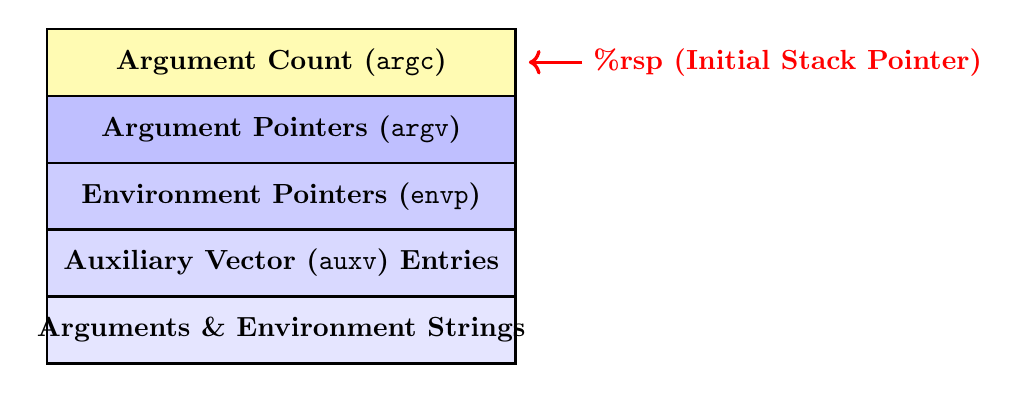
\begin{tikzpicture}[scale=0.85]
    \draw[thick, fill=blue!10] (0, 0) rectangle (7, 1) node[pos=.5] {\textbf{Arguments \& Environment Strings}};
    \draw[thick, fill=blue!15] (0, 1) rectangle (7, 2) node[pos=.5] {\textbf{Auxiliary Vector (\texttt{auxv}) Entries}};
    \draw[thick, fill=blue!20] (0, 2) rectangle (7, 3) node[pos=.5] {\textbf{Environment Pointers (\texttt{envp})}};
    \draw[thick, fill=blue!25] (0, 3) rectangle (7, 4) node[pos=.5] {\textbf{Argument Pointers (\texttt{argv})}};
    \draw[thick, fill=yellow!30] (0, 4) rectangle (7, 5) node[pos=.5] {\textbf{Argument Count (\texttt{argc})}};
    \draw[->, very thick, red] (8, 4.5) -- (7.2, 4.5) node[right, pos=0, red] {\textbf{\%rsp (Initial Stack Pointer)}};
\end{tikzpicture}
\caption{System V AMD64 Initial Process Stack Layout.}
\label{fig:user_stack_layout}
\end{figure}

The auxiliary vector communicates runtime information from the kernel to the dynamic linker:
\begin{itemize}
    \item \texttt{AT\_PHDR}: Virtual base address of the Program Header Table;
    \item \texttt{AT\_PHNUM}: Number of program header entries;
    \item \texttt{AT\_ENTRY}: Executable entry point;
    \item \texttt{AT\_PAGESZ}: System hardware page size (4096 bytes);
    \item \texttt{AT\_RANDOM}: 16 bytes of cryptographically secure random values (for stack canaries).
\end{itemize}

% ==============================================================================
\section{Summary}
\label{sec:summary_chap2}
% ==============================================================================

Processes and threads are the core abstractions of concurrent operating systems. A process provides an isolated virtual address space and kernel resources, while threads provide concurrent execution contexts sharing that memory. 

To prevent race conditions, critical regions must be protected through mutual exclusion primitives, ranging from atomic hardware instructions (\texttt{lock cmpxchg}) to user-space futexes. Hydra coordinates execution through a priority-aware preemptive scheduler running at 100~Hz with dynamic starvation prevention, executing context switches by saving complete \texttt{TaskRegisters} and manipulating x86\_64 \texttt{CR3} and \texttt{FS\_BASE} registers. Finally, synchronous rendezvous IPC provides mathematically failure-isolated communication across Ring~3 system servers.

% ==============================================================================
\section{Exercises and Review Problems}
\label{sec:exercises_chap2}
% ==============================================================================

\begin{enumerate}
    \item \textbf{Process vs. Thread:} What state is shared between multiple threads executing within the same process? What state must remain strictly private to each thread?
    \item \textbf{Context Switch Mechanics:} During an x86\_64 interrupt, which registers are pushed onto the stack automatically by the CPU hardware, and which registers must be preserved by the operating system software stub?
    \item \textbf{Address Space Invalidation:} Why does writing a new physical address into \texttt{CR3} degrade subsequent memory access performance for a few hundred CPU cycles? How do modern processors mitigate this penalty?
    \item \textbf{Race Conditions:} Write a short pseudo-code snippet illustrating how two threads concurrently executing \texttt{counter = counter + 1} can lose an update if preempted at the machine instruction level.
    \item \textbf{Peterson's Algorithm:} Explain how Peterson's two-process mutual exclusion algorithm functions. Why does it fail on modern multi-core x86\_64 processors unless hardware memory fences (\texttt{mfence}) are inserted?
    \item \textbf{Futex Efficiency:} Why are Linux-compatible futexes dramatically faster than traditional UNIX semaphore system calls in the uncontended locking case?
    \item \textbf{Starvation Prevention:} In Hydra's scheduler, how does the \texttt{STARVATION\_LIMIT} parameter ensure that low-priority batch threads eventually make progress even in the presence of continuous high-priority network traffic?
    \item \textbf{Deadlock Analysis:} State the four necessary conditions for deadlock (Coffman conditions). Which condition is broken by Dijkstra's resource ordering solution to the Dining Philosophers Problem?
    \item \textbf{CPU Power Management:} What does the assembly instruction \texttt{hlt} do? Why is it vital that interrupts be re-enabled (\texttt{sti}) immediately prior to halting the CPU inside the idle task loop?
    \item \textbf{Design Problem:} Design an asynchronous message-passing IPC system with bounded mailboxes. What happens when a mailbox becomes full? How does your design compare to Hydra's synchronous rendezvous model in terms of memory footprint and susceptibility to denial-of-service attacks?
\end{enumerate}

\chapter{Memory Management}
\label{chap:memory}

Memory is the lifeblood of an operating system. While processor clock frequencies and execution pipelines have advanced exponentially over the past four decades, the latency and bandwidth of main memory (DRAM) have struggled to keep pace. To maintain system performance while providing robust security, modern computing architectures rely on a deep hierarchy of memory mechanisms: L1, L2, and L3 processor caches backed by hardware-enforced \textbf{Virtual Memory}.

Virtual memory fulfills two foundational requirements in modern operating systems:
\begin{enumerate}
    \item \textbf{Process Protection and Isolation:} Every process is granted the illusion of owning a contiguous, multi-terabyte address space. A process cannot inspect, modify, or corrupt the memory of another process or the microkernel, because it possesses no capability to name or address those physical frames.
    \item \textbf{Transparent Resource Multiplexing:} Physical memory does not need to be allocated contiguously, nor does an application's entire address space need to reside in physical RAM simultaneously. Pages can be loaded lazily on demand, shared transparently via Copy-on-Write (CoW), or mapped directly to peripheral devices for high-speed Direct Memory Access (DMA).
\end{enumerate}

In this chapter, we explore how Hydra implements physical frame allocation, manages x86\_64 4-level page tables, dispatches page faults (\texttt{\#PF}), and powers userland memory management through POSIX-compatible \texttt{mmap} and shared memory abstractions.

% ==============================================================================
\section{Foundations of Memory Management}
\label{sec:mem_foundations}
% ==============================================================================

To appreciate the elegance of modern hardware paging, one must first examine the historical solutions developed by operating system designers.

\subsection{Monoprogramming without Swapping or Paging}
In early batch computing and rudimentary personal computer operating systems (such as CP/M and MS-DOS), only a single program ran at any given moment. Memory was divided simply into a region reserved for the operating system (in ROM or low RAM) and the remainder allocated to the active user application.
\begin{itemize}
    \item If the user program contained a bug that overwrote low memory, the operating system was destroyed, requiring a hard machine reboot.
    \item Concurrency was impossible: one program had to exit completely before another could begin.
\end{itemize}

\subsection{Multiprogramming with Fixed and Variable Partitions}
With the advent of timesharing, memory was divided into discrete partitions. In \textbf{fixed partitioning}, memory was segmented into predetermined blocks (e.g., 100~KiB, 200~KiB, 500~KiB). Incoming programs were queued for the smallest partition capable of accommodating them.
\begin{itemize}
    \item This introduced severe \textbf{internal fragmentation}: a 105~KiB job placed in a 200~KiB partition wasted 95~KiB of allocated memory.
\end{itemize}

In \textbf{variable partitioning}, the operating system allocated exactly the memory requested by each program. However, as programs terminated and new ones arrived, memory became riddled with tiny, unusable gaps between active allocations---a pathology known as \textbf{external fragmentation}.

\subsection{Dynamic Relocation and Base/Limit Registers}
To prevent programs from corrupting each other, early hardware introduced \textbf{Base and Limit registers}:
\begin{itemize}
    \item When the CPU scheduled a program, the kernel loaded its physical start address into the Base register and its allocation size into the Limit register.
    \item On every instruction, hardware automatically added the Base register to the program's relative address and verified that the result did not exceed the Limit register.
\end{itemize}
While this provided basic spatial protection, it required that every program occupy a single, contiguous block of physical RAM. If a program needed to grow its heap or stack dynamically, or if physical RAM was exhausted, the operating system was forced to \textbf{swap} the entire process out to a mechanical disk drive, halting execution for hundreds of milliseconds.

% ==============================================================================
\section{The x86\_64 4-Level Paging Architecture}
\label{sec:paging_arch}
% ==============================================================================

Modern 64-bit architectures abandon contiguous physical allocations entirely in favor of \textbf{Paging}. The physical memory of the computer is partitioned into uniform, fixed-size chunks called \textbf{Physical Frames} (typically 4096 bytes or 4~KiB). Similarly, a process's virtual memory is divided into fixed-size units called \textbf{Virtual Pages}. A virtual page may be mapped to any physical frame anywhere in RAM, or left unmapped entirely.

\subsection{Canonical Virtual Addresses and the 48-Bit Address Space}
Although x86\_64 general-purpose registers (\texttt{RAX}, \texttt{RSP}, \texttt{RIP}) are 64 bits wide, current hardware does not implement a full 64-bit physical or virtual address bus ($2^{64} = 16\text{ Exabytes}$). Instead, the architecture implements a **48-bit virtual address space**, spanning $2^{48} = 256\text{ Terabytes}$.

To prevent software from using the upper 16 unused bits for arbitrary pointer tagging (which would cause forward compatibility breaks when processors expand to 57-bit 5-level paging), the hardware enforces **Canonical Addressing**:
\begin{itemize}
    \item Bits 47 through 63 must be identical (a sign-extension of bit 47).
    \item If bit 47 is \texttt{0}, bits 48 through 63 must all be \texttt{0} (the Lower Half: \texttt{0x0000\_0000\_0000\_0000} to \texttt{0x0000\_7FFF\_FFFF\_FFFF}). This region is reserved for user-space processes.
    \item If bit 47 is \texttt{1}, bits 48 through 63 must all be \texttt{1} (the Upper Half: \texttt{0xFFFF\_8000\_0000\_0000} to \texttt{0xFFFF\_FFFF\_FFFF\_FFFF}). This region is reserved for the operating system kernel.
    \item Any attempt to dereference a non-canonical address (e.g., \texttt{0x0001\_0000\_0000\_0000}) triggers an immediate General Protection Fault (\texttt{\#GP}, Exception 13).
\end{itemize}

\subsection{The 4-Level Page Table Translation Walk}
The translation of a 48-bit canonical virtual address into a physical address is performed by the hardware Memory Management Unit (MMU) via a 4-level hierarchical walk:
\begin{enumerate}
    \item \textbf{Level 4 (PML4):} Page Map Level 4 Table.
    \item \textbf{Level 3 (PDPT):} Page Directory Pointer Table.
    \item \textbf{Level 2 (PD):} Page Directory Table.
    \item \textbf{Level 1 (PT):} Page Table.
\end{enumerate}

Every table at each of the four levels contains exactly \textbf{512 entries}, each 8 bytes (64 bits) wide. Thus, every individual table occupies exactly one 4096-byte physical frame ($512 \times 8 = 4096$).

\begin{figure}[htbp]
\centering
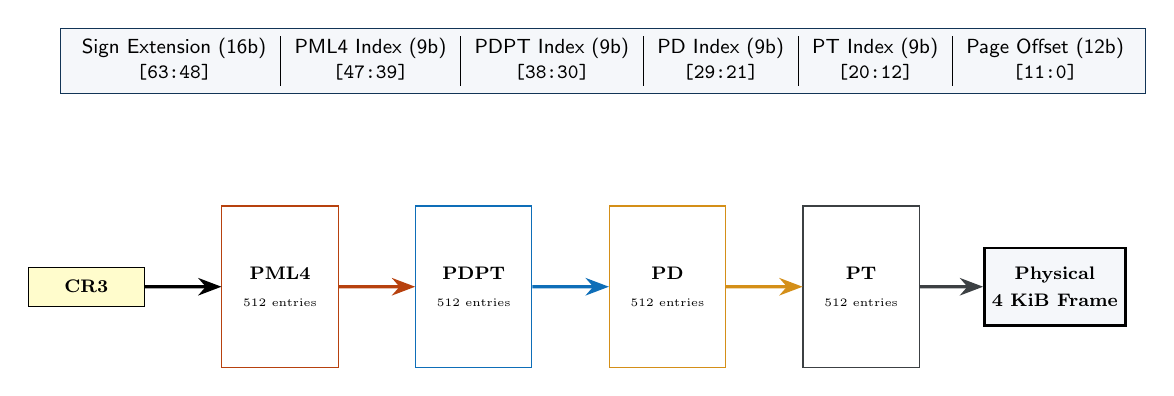
\begin{tikzpicture}[scale=0.82, every node/.style={transform shape}]
    % Virtual Address decomposition
    \node[draw=hydrablue, fill=hydralight, font=\small\sffamily, minimum width=13cm, minimum height=0.8cm] (va) at (6.5, 6) {
        \begin{tabular}{c|c|c|c|c|c}
            Sign Extension (16b) & PML4 Index (9b) & PDPT Index (9b) & PD Index (9b) & PT Index (9b) & Page Offset (12b) \\
            \texttt{[63:48]} & \texttt{[47:39]} & \texttt{[38:30]} & \texttt{[29:21]} & \texttt{[20:12]} & \texttt{[11:0]}
        \end{tabular}
    };

    % Tables
    \node[draw=rustred, fill=white, minimum width=1.8cm, minimum height=2.5cm, align=center] (pml4) at (1.5, 2.5) {\footnotesize \textbf{PML4}\\ \tiny 512 entries};
    \node[draw=rustkeyword, fill=white, minimum width=1.8cm, minimum height=2.5cm, align=center] (pdpt) at (4.5, 2.5) {\footnotesize \textbf{PDPT}\\ \tiny 512 entries};
    \node[draw=hydragold, fill=white, minimum width=1.8cm, minimum height=2.5cm, align=center] (pd) at (7.5, 2.5) {\footnotesize \textbf{PD}\\ \tiny 512 entries};
    \node[draw=hydragray, fill=white, minimum width=1.8cm, minimum height=2.5cm, align=center] (pt) at (10.5, 2.5) {\footnotesize \textbf{PT}\\ \tiny 512 entries};
    \node[draw=black, fill=hydralight, line width=1pt, minimum width=2.0cm, minimum height=1.2cm, align=center] (frame) at (13.5, 2.5) {\footnotesize \textbf{Physical}\\\footnotesize \textbf{4 KiB Frame}};

    % CR3
    \node[draw=black, fill=yellow!20, minimum width=1.8cm, minimum height=0.6cm] (cr3) at (-1.5, 2.5) {\footnotesize \textbf{CR3}};

    \draw[->, >=Stealth, line width=1.2pt] (cr3) -- (pml4);
    \draw[->, >=Stealth, line width=1.2pt, rustred] (pml4) -- (pdpt);
    \draw[->, >=Stealth, line width=1.2pt, rustkeyword] (pdpt) -- (pd);
    \draw[->, >=Stealth, line width=1.2pt, hydragold] (pd) -- (pt);
    \draw[->, >=Stealth, line width=1.2pt, hydragray] (pt) -- (frame);
\end{tikzpicture}
\caption{The x86\_64 4-Level Page Table Translation Walk.}
\label{fig:page_walk}
\end{figure}

The MMU hardware evaluates a virtual address through the following sequential steps:
\begin{enumerate}
    \item The physical base address of the PML4 table is retrieved from the \textbf{\texttt{CR3}} control register.
    \item Bits 47:39 ($9\text{ bits} = 512\text{ indices}$) index into the PML4 table to find the physical address of the PDPT.
    \item Bits 38:30 ($9\text{ bits}$) index into the PDPT to find the physical address of the Page Directory (PD).
    \item Bits 29:21 ($9\text{ bits}$) index into the PD to find the physical address of the Page Table (PT).
    \item Bits 20:12 ($9\text{ bits}$) index into the PT to locate the target 64-bit Page Table Entry (PTE), which yields the physical frame base address.
    \item Bits 11:0 ($12\text{ bits} = 4096\text{ byte offsets}$) are concatenated with the physical frame address to form the final 52-bit physical address presented to the memory controller.
\end{enumerate}

\subsection{Page Table Entry (PTE) Bitflags}
Every 64-bit entry across all four paging levels contains hardware status and control flags:

\begin{lstlisting}[language=Rust, caption={Page Table Entry Bitflags in Hydra (\texttt{src/memory/paging.rs})}]
bitflags::bitflags! {
    pub struct PageTableFlags: u64 {
        const PRESENT       = 1 << 0;  // Frame is present in physical RAM
        const WRITABLE      = 1 << 1;  // Page is writable (read-only if unset)
        const USER          = 1 << 2;  // Accessible from Ring 3 userland
        const WRITE_THROUGH = 1 << 3;  // Caching: write-through to DRAM
        const NO_CACHE      = 1 << 4;  // Caching disabled (used for MMIO)
        const ACCESSED      = 1 << 5;  // Set by hardware MMU on read/write
        const DIRTY         = 1 << 6;  // Set by hardware MMU on write
        const HUGE_PAGE     = 1 << 7;  // 2 MiB (PD) or 1 GiB (PDPT) huge page
        const GLOBAL        = 1 << 8;  // Retained in TLB across CR3 reload
        const NO_EXECUTE    = 1 << 63; // Instruction execution disabled (NX)
    }
}
\end{lstlisting}

\begin{itemize}
    \item \textbf{The User/Supervisor Bit (Bit 2):} If bit 2 is \texttt{0}, user-space code running in Ring~3 cannot read or write the page; any attempt triggers a Page Fault. This enforces kernel memory privacy.
    \item \textbf{The No-Execute (NX) Bit (Bit 63):} Enabled via MSR \texttt{EFER.NXE}. When set, any attempt by the CPU instruction decoder to fetch instructions from this memory page raises a Page Fault. This renders buffer-overflow exploits unable to execute injected shellcode on stacks or heaps.
\end{itemize}

% ==============================================================================
\section{The Translation Lookaside Buffer (TLB)}
\label{sec:tlb_deep}
% ==============================================================================

Translating a virtual address via a 4-level page table requires four sequential DRAM accesses simply to locate the target physical frame before the application's actual data can be read. Because DRAM latency is roughly 50 to 100 nanoseconds, performing four DRAM reads on every memory instruction would slow the processor down by a factor of five.

To eliminate this overhead, modern CPUs incorporate a specialized associative hardware cache called the \textbf{Translation Lookaside Buffer (TLB)}.

\subsection{TLB Operation and Hit Rates}
The TLB stores recently translated virtual-page-to-physical-frame mappings directly on the CPU die:
\begin{itemize}
    \item On every instruction, the MMU checks the TLB in parallel.
    \item If the mapping is present (\textbf{TLB Hit}), the physical address is generated in less than 1 nanosecond (a single clock cycle).
    \item If the mapping is absent (\textbf{TLB Miss}), the hardware page table walker performs the full 4-level DRAM walk, stores the resulting translation into the TLB, and completes the access.
\end{itemize}

Because programs exhibit high \textbf{temporal locality} (repeatedly accessing the same variables and loop code) and \textbf{spatial locality} (accessing adjacent array elements), typical TLB hit rates exceed 99\%.

\subsection{TLB Invalidation and \texttt{invlpg}}
When the operating system modifies a page table entry---such as unmapping a page, changing permissions from read-write to read-only during Copy-on-Write, or recycling a physical frame---the cached translation in the TLB becomes stale and dangerous.

The kernel must explicitly invalidate the stale TLB entry using the privileged x86 assembly instruction \texttt{invlpg}:
\begin{lstlisting}[language=Rust, caption={Invalidating a Single Page in the TLB (\texttt{src/memory/paging.rs})}]
pub fn invalidate_tlb_page(addr: VirtAddr) {
    unsafe {
        core::arch::asm!(
            "invlpg [{0}]",
            in(reg) addr.as_u64(),
            options(nostack, preserves_flags)
        );
    }
}
\end{lstlisting}

\subsection{Global Pages and PCIDs}
Historically, loading a new physical address into \texttt{CR3} during a process context switch automatically flushed the entire TLB, destroying all cached translations. Modern x86\_64 processors provide two hardware mechanisms to eliminate this penalty:
\begin{enumerate}
    \item \textbf{Global Pages (\texttt{PGE}, bit 7 of \texttt{CR4}):} When the \texttt{GLOBAL} bit (bit 8) is set in a PTE, that mapping represents shared kernel code. The CPU retains global pages in the TLB across \texttt{CR3} reloads.
    \item \textbf{Process-Context Identifiers (PCID, bit 17 of \texttt{CR4}):} Hardware tags every TLB entry with a 12-bit address space ID. When switching between tasks, the kernel changes the active PCID in \texttt{CR3} without flushing entries belonging to other processes.
\end{enumerate}

% ==============================================================================
\section{Physical Frame Allocation: The Hydra Architecture}
\label{sec:frame_alloc_deep}
% ==============================================================================

Before an operating system can construct page tables, it must know which physical memory frames exist, which are reserved by motherboard hardware (such as ACPI tables, PCI Express MMIO apertures, and video framebuffers), and which are available for allocation.

\subsection{Parsing the UEFI Memory Map}
Hydra boots under modern UEFI firmware. During early boot, the kernel queries the UEFI Boot Services table via \texttt{get\_memory\_map()}:

\begin{lstlisting}[language=Rust, caption={Harvesting Conventional Memory from UEFI (\texttt{src/arch/boot\_services.rs})}]
let memory_map = uefi_boot_services.get_memory_map()?;
for descriptor in memory_map.entries() {
    if descriptor.ty == MemoryType::CONVENTIONAL {
        let start_frame = descriptor.phys_start / PAGE_SIZE;
        let frame_count = descriptor.page_count;
        frame_allocator.register_region(start_frame, frame_count);
    }
}
\end{lstlisting}

Regions marked as \texttt{MemoryType::CONVENTIONAL} represent clean, usable system RAM. Regions marked as \texttt{ACPI\_RECLAIM}, \texttt{RESERVED}, or \texttt{RUNTIME\_SERVICES} are strictly excluded from allocation.

\subsection{The Intrusive $O(1)$ Free List Allocator}
In Hydra's \texttt{PhysicalMemoryManager} (\texttt{src/memory/frame\_allocator.rs}), memory allocation is optimized for zero runtime metadata overhead:
\begin{enumerate}
    \item \textbf{Bump Pointer for Fresh Frames:} Physical memory descriptors harvested from UEFI are initially carved using a fast monotonic bump pointer.
    \item \textbf{Intrusive Free List for Recycled Frames:} When an application terminates or frees virtual pages, the returned 4096-byte physical frame is recycled onto an intrusive singly-linked list.
    \begin{itemize}
        \item Because the frame is currently unused by any process, the kernel stores the 64-bit physical address of the \textit{next} free frame directly within the first 8 bytes of the freed frame itself!
        \item When allocating a new frame, the allocator pops the head of this intrusive free list in $O(1)$ time. Only if the free list is empty does the allocator bump the physical memory descriptor.
    \end{itemize}
    \item \textbf{Reference Counting Table:} To support Copy-on-Write and shared memory maps, Hydra maintains a 16-bit reference counter for every managed user frame. When a page is shared across multiple processes, its reference count is incremented via \texttt{frame\_ref\_inc()}; when unmapped, it is decremented via \texttt{frame\_ref\_dec()}. The physical frame is returned to the intrusive free list only when its reference count drops to zero.
\end{enumerate}

% ==============================================================================
\section{Page Fault Handling (\#PF) and Copy-on-Write}
\label{sec:page_fault_handling}
% ==============================================================================

A \textbf{Page Fault} is not necessarily an error. Rather, it is a high-speed hardware notification that the executing program requires operating system intervention to resolve an address mapping.

\subsection{Hardware Exception Mechanics}
When the CPU encounters a virtual address where the \texttt{PRESENT} bit is \texttt{0}, or attempts an operation that violates permissions (e.g., writing to a page where \texttt{WRITABLE=0}, or executing code where \texttt{NO\_EXECUTE=1}), it halts instruction execution and raises **Exception 14 (\#PF)**:
\begin{enumerate}
    \item The CPU loads the faulting linear virtual address into the \textbf{\texttt{CR2}} control register.
    \item The CPU pushes a 32-bit hardware error code onto the stack, encoding the exact nature of the fault:
\end{enumerate}

\begin{table}[htbp]
\centering
\small
\begin{tabular}{lll}
\hline
\textbf{Bit} & \textbf{Flag} & \textbf{Diagnostic Meaning when Set} \\
\hline
Bit 0 & \texttt{P (Present)} & Protection fault (page was present, but violated permissions) \\
Bit 1 & \texttt{W/R (Write)} & Access caused by a write instruction (read if 0) \\
Bit 2 & \texttt{U/S (User)} & Access originated from Ring 3 user space (Ring 0 supervisor if 0) \\
Bit 3 & \texttt{RSVD (Reserved)} & Reserved bit set in page table entry (corrupt page table) \\
Bit 4 & \texttt{I/D (Instruction)} & Fault caused by an instruction fetch (NX bit violation) \\
Bit 5 & \texttt{PK (Protection Key)} & Memory protection key violation \\
\hline
\end{tabular}
\caption{Architectural x86\_64 Page Fault Error Code Flags.}
\label{tab:pf_flags}
\end{table}

\subsection{The Anatomy of Copy-on-Write (CoW)}
In traditional UNIX, invoking \texttt{fork()} required the kernel to immediately allocate fresh physical frames for the entire child process and copy every byte of memory from the parent. For a 2~GiB process, this operation wasted hundreds of milliseconds and gigabytes of RAM---especially considering that over 90\% of \texttt{fork()} calls are immediately followed by an \texttt{execve()} that discards the child's address space!

Hydra implements high-performance **Copy-on-Write (CoW)**:
\begin{enumerate}
    \item \textbf{Fork Phase:} When a process forks, Hydra clones the parent's PML4 page tables. For every writable user page, Hydra:
    \begin{itemize}
        \item Clears the \texttt{WRITABLE} bit in both parent and child PTEs;
        \item Sets a software marker flag (\texttt{COW});
        \item Increments the physical frame's reference count in the frame allocator table.
    \end{itemize}
    This operation takes mere microseconds because \textbf{zero memory is copied}.
    \item \textbf{Fault Phase:} As long as both parent and child only read their memory, execution proceeds at native hardware speed.
    \item \textbf{Copy Phase:} When either process attempts to write to a shared page, the CPU detects \texttt{WRITABLE=0} and raises a Page Fault (\#PF) with error code $P=1, W=1, U=1$.
    \item \textbf{Resolution Phase:} The Hydra fault handler reads \texttt{CR2}:
    \begin{itemize}
        \item If the frame's reference count is 1 (the other process already made its copy), Hydra simply restores \texttt{WRITABLE=1} and returns.
        \item If the reference count is $> 1$, Hydra allocates a single fresh physical frame, copies 4096 bytes from the shared frame into the new frame, decrements the shared frame's reference count, updates the faulting process's PTE to point to the new frame with \texttt{WRITABLE=1}, and flushes the TLB via \texttt{invlpg}.
    \end{itemize}
    \item \textbf{Resume:} The CPU retries the write instruction, which now succeeds immediately.
\end{enumerate}

% ==============================================================================
\section{Page Replacement Algorithms}
\label{sec:page_replacement}
% ==============================================================================

When all physical memory frames are occupied and an application demands additional pages, the operating system must select an existing resident page, evict it (writing it to swap storage if dirty), and reuse its physical frame.

\subsection{Belady's Optimal Algorithm}
In 1966, Sheldon Belady demonstrated the theoretical optimal page replacement algorithm: evict the page that will not be referenced for the longest period of time in the future. While impossible to implement in a real general-purpose operating system (because the kernel cannot predict the future), Belady's algorithm serves as the gold standard against which all real-world algorithms are measured.

\subsection{The Least Recently Used (LRU) Algorithm}
A practical approximation of the optimal algorithm is **Least Recently Used (LRU)**: evict the page that has remained unreferenced for the longest duration in the past. 
\begin{itemize}
    \item True LRU requires hardware to maintain a 64-bit timestamp or matrix for every single memory access, which is too expensive for modern CPUs.
    \item Operating systems approximate LRU using the hardware \textbf{Accessed (A)} and \textbf{Dirty (D)} bits in the Page Table Entry.
\end{itemize}

\subsection{The Clock Algorithm and WSClock}
A standard approximation is the **Clock Algorithm** (Figure~\ref{fig:clock_algorithm}):
\begin{enumerate}
    \item All candidate physical pages are organized in a logical circular linked list, like the face of a clock. A hand points to the oldest page.
    \item When a page fault requires an eviction, the kernel inspects the page pointed to by the hand:
    \begin{itemize}
        \item If its Accessed bit $A = 1$, the page was recently referenced. The kernel clears $A \leftarrow 0$, advances the clock hand to the next page, and repeats.
        \item If its Accessed bit $A = 0$, the page has not been referenced since the last sweep. This page is selected for eviction. If its Dirty bit $D = 1$, it is scheduled for asynchronous write-back to disk; if $D = 0$, its frame is reclaimed immediately!
    \end{itemize}
\end{enumerate}

\begin{figure}[htbp]
\centering
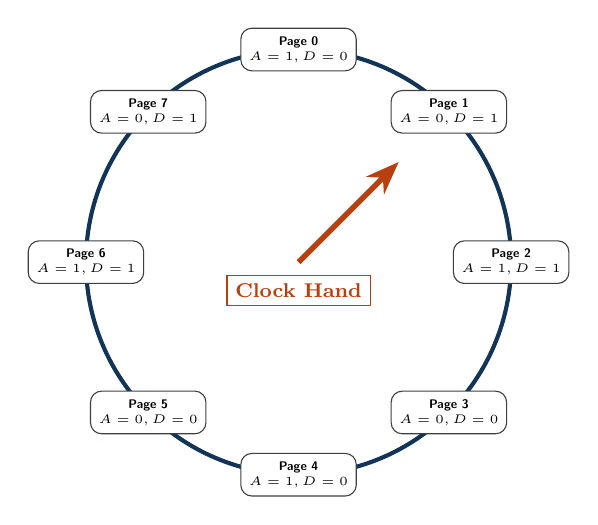
\begin{tikzpicture}[scale=0.9, every node/.style={transform shape}]
    % Clock face
    \draw[line width=1.5pt, hydrablue] (0,0) circle (3.0cm);
    
    % Clock entries
    \foreach \angle/\num/\a/\d in {
        90/Page 0/1/0,
        45/Page 1/0/1,
        0/Page 2/1/1,
        315/Page 3/0/0,
        270/Page 4/1/0,
        225/Page 5/0/0,
        180/Page 6/1/1,
        135/Page 7/0/1
    } {
        \node[draw=hydragray, fill=white, rounded corners, font=\tiny\sffamily, align=center] at (\angle:3.0cm) {
            \textbf{\num}\\
            $A=\a, D=\d$
        };
    }
    
    % Hand
    \draw[->, >=Stealth, line width=2pt, rustred] (0,0) -- (45:2.0cm);
    \node[fill=white, draw=rustred, font=\footnotesize\bfseries\color{rustred}] at (0, -0.4) {Clock Hand};
\end{tikzpicture}
\caption{The Circular Clock Page Replacement Algorithm.}
\label{fig:clock_algorithm}
\end{figure}

% ==============================================================================
\section{Kernel Heap Management: Slab and Buddy Allocators}
\label{sec:kernel_heap}
% ==============================================================================

While the physical frame allocator manages memory at 4096-byte page granularity, the microkernel core requires dynamic memory allocations for structures of arbitrary sizes: 32-byte IPC messages, 256-byte TCB descriptors, 64-byte file paths, and dynamically resizing vectors (\texttt{Vec<T>}).

Hydra implements a dual-layer kernel heap allocator in \texttt{src/memory/heap.rs}:
\begin{enumerate}
    \item \textbf{The Buddy Allocator:} Manages contiguous multi-page power-of-two blocks ($4\text{ KiB}, 8\text{ KiB}, 16\text{ KiB}, \dots, 2\text{ MiB}$). When a block of size $2^k$ is freed, the allocator inspects its adjacent "buddy" block in physical memory. If the buddy is also free, they are coalesced into a single larger block of size $2^{k+1}$, eliminating external fragmentation.
    \item \textbf{The Slab Allocator (Bonwick):} Carves large buddy pages into pre-allocated caches of fixed-size object slots (e.g., 32B, 64B, 128B, 256B, 512B slabs). Allocating an object requires no search: the kernel simply pops the head of the slab's freelist in $O(1)$ time, perfectly avoiding internal fragmentation for small kernel structs.
\end{enumerate}

\subsection{The Size-Class Free List Cache (\texttt{src/memory/heap.rs})}

To minimize lock contention and memory fragmentation, the Hydra kernel heap organizes allocations into eight discrete power-of-two size classes:
\begin{equation}
\mathcal{C} = \{16, 32, 64, 128, 256, 512, 1024, 2048\} \text{ bytes}
\end{equation}

When an allocation request arrives, the size is rounded up to the nearest class boundary. Each class maintains a private lock-free singly-linked free list:

\begin{lstlisting}[language=Rust, caption={Size-Class Kernel Heap Allocator (\texttt{src/memory/heap.rs})}]
pub const HEAP_SIZE: usize = 1024 * 1024 * 1024; // 1024 MiB
const CLASS_SIZES: [usize; 8] = [16, 32, 64, 128, 256, 512, 1024, 2048];
const REFILL_BYTES: usize = 16 * 1024; // 16 KiB refill chunk

pub struct SizeClassHeap {
    free_lists: [spin::Mutex<Option<*mut FreeNode>>; 8],
    fallback: linked_list_allocator::LockedHeap,
}

impl SizeClassHeap {
    /// Allocates memory from the appropriate size-class cache.
    pub unsafe fn allocate(&self, layout: core::alloc::Layout) -> *mut u8 {
        let size = layout.size().max(layout.align());

        // Find smallest size class that accommodates the request
        if let Some(idx) = CLASS_SIZES.iter().position(|&s| s >= size) {
            let mut list = self.free_lists[idx].lock();
            if let Some(node) = *list {
                *list = (*node).next;
                return node as *mut u8;
            }

            // Free list empty: refill by carving a 16 KiB block from fallback heap
            self.refill_class(idx, &mut list);
            if let Some(node) = *list {
                *list = (*node).next;
                return node as *mut u8;
            }
        }

        // Large allocations (> 2048 B) fall back to the main locked heap
        self.fallback.lock().allocate_first_fit(layout)
            .ok()
            .map_or(core::ptr::null_mut(), |p| p.as_ptr())
    }

    /// Deallocates memory, returning it to the appropriate size-class free list.
    pub unsafe fn deallocate(&self, ptr: *mut u8, layout: core::alloc::Layout) {
        let size = layout.size().max(layout.align());

        if let Some(idx) = CLASS_SIZES.iter().position(|&s| s >= size) {
            let mut list = self.free_lists[idx].lock();
            let node = ptr as *mut FreeNode;
            (*node).next = *list;
            *list = Some(node);
            return;
        }

        self.fallback.lock().deallocate(core::ptr::NonNull::new_unchecked(ptr), layout);
    }
}
\end{lstlisting}

\subsection{Memory Poisoning and Use-After-Free Detection}

During kernel development and testing, silent heap corruption represents a lethal hazard. When enabled, Hydra's heap allocator implements \textbf{Memory Poisoning}:
\begin{itemize}
    \item When an object is deallocated via \texttt{kfree()}, its entire memory body is overwritten with the poison byte pattern \texttt{0xDD}.
    \item When an object is reallocated, the allocator verifies that every byte still matches \texttt{0xDD}.
    \item If any byte deviates from \texttt{0xDD}, a wild write or use-after-free occurred while the memory was in the free list! The kernel immediately halts and prints the corruption address and stack trace to the console.
\end{itemize}

% ==============================================================================
\section{Summary}
\label{sec:summary_chap3}
% ==============================================================================

Memory management on modern architectures coordinates physical frames and virtual pages through hardware MMU translation. Standard x86\_64 Long Mode translates 48-bit canonical virtual addresses through a 4-level page table hierarchy (PML4, PDPT, PD, PT) into 4~KiB physical frames. The Translation Lookaside Buffer (TLB) caches these translations, delivering near single-cycle memory access.

Hydra harvests usable physical RAM directly from the UEFI memory map, managing frames via an intrusive $O(1)$ singly-linked free list and per-frame reference counts. Page faults (\#PF) drive lazy demand paging and Copy-on-Write address space cloning. Finally, kernel heap allocations are multiplexed through slab and buddy allocators, ensuring bounded allocation latencies across all microkernel subsystems.

% ==============================================================================
\section{Exercises and Review Problems}
\label{sec:exercises_chap3}
% ==============================================================================

\begin{enumerate}
    \item \textbf{Canonical Addressing:} Why does the x86\_64 architecture require bits 48 through 63 of a virtual address to be a sign-extension of bit 47? What happens if user-space software attempts to dereference \texttt{0x0002\_0000\_0000\_0000}?
    \item \textbf{Mathematical Paging:} Calculate the maximum physical memory addressable by a standard 4-level x86\_64 page table where each Page Table Entry is 64 bits wide and physical frame pointers are 52 bits wide.
    \item \textbf{Paging Walk:} Given the virtual address \texttt{0x0000\_7FFF\_DEAD\_BEEF}, decompose this address into its 9-bit PML4 index, PDPT index, PD index, PT index, and 12-bit page offset.
    \item \textbf{TLB Hit Math:} Suppose a memory access takes 1~nanosecond on a TLB hit and 60~nanoseconds on a TLB miss (requiring four DRAM page table reads). If the system achieves a 98\% TLB hit rate, calculate the effective memory access time (EMAT).
    \item \textbf{Copy-on-Write:} Detail the sequence of hardware and software events that occur when a child process writes to a Copy-on-Write page. Under what exact condition can the kernel avoid allocating a new physical frame?
    \item \textbf{Page Fault Flags:} A user thread attempts to execute machine code located on its stack. What bits will be set in the resulting x86\_64 Page Fault error code pushed onto the kernel stack?
    \item \textbf{Fragmentation Analysis:} Distinguish between internal fragmentation and external fragmentation. How does a slab allocator eliminate both forms of fragmentation when allocating small kernel structs?
    \item \textbf{Belady's Anomaly:} What is Belady's Anomaly? Name a page replacement algorithm that is susceptible to it, and name one that is mathematically proven to be immune.
    \item \textbf{Buddy Allocation:} Consider a Buddy Allocator managing 1024~KiB of memory. Show the state of the allocation tree after the following sequence of requests: Allocate 70~KiB, Allocate 200~KiB, Allocate 60~KiB, Free the 70~KiB allocation.
    \item \textbf{Design Problem:} Modern processors support "Huge Pages" (2~MiB pages at Level~2 and 1~GiB pages at Level~3). What changes to the page table structure are required to configure a 2~MiB huge page? What are the advantages and disadvantages of using 2~MiB huge pages for database buffer caches?
\end{enumerate}


\part{Storage, I/O \& Networking}
\chapter{File Systems and Enterprise Storage: The OpenZFS Deep Dive}
\label{chap:zfs}

In classical operating systems literature---including Andrew Tanenbaum's dissection of the MINIX file system~\cite{tanenbaum2006operating}---file systems are depicted as static disk structures: a boot block, a superblock, an inode bitmap, a zone bitmap, an array of fixed-size inodes, and data blocks.

While conceptually straightforward, traditional file systems suffer from fatal structural liabilities in production environments:
\begin{enumerate}
    \item \textbf{Silent Data Corruption (Bit Rot):} Magnetic decay, cosmic rays, firmware bugs, or bus errors can flip bits in storage media. Traditional file systems have no mechanism to detect when a sector read from disk differs from what was originally written.
    \item \textbf{Destructive In-Place Overwrites:} When writing to an existing file, old data blocks and inode metadata are overwritten directly. An unexpected power failure or system reset mid-write leaves the file system in an inconsistent state, requiring lengthy, error-prone \texttt{fsck} recovery.
    \item \textbf{Rigid Partition Boundaries:} Physical disks are partitioned into fixed slices. If the \texttt{/usr} partition fills up while \texttt{/home} has 500~GB of empty space, the user must repartition the entire drive.
\end{enumerate}

To overcome these liabilities, Hydra implements a complete, native **OpenZFS** enterprise storage engine directly within its microkernel hierarchy. In this chapter, we dissect file system principles, ZFS storage pools, Copy-on-Write transactions, Merkle tree checksumming, dnodes, and the Ring~3 storage server architecture.

% ==============================================================================
\section{File System Fundamentals: Abstractions and Operations}
\label{sec:fs_fundamentals}
% ==============================================================================

From the user's perspective, a file system provides long-term persistence for data and programs. Unlike physical RAM, which is volatile and lost upon power failure, magnetic and solid-state storage media retain information indefinitely.

\subsection{File Concepts, Naming, and Types}
A \textbf{file} is an abstract data type consisting of a named sequence of bytes. Operating systems categorize files into distinct types:
\begin{itemize}
    \item \textbf{Regular Files:} Contain arbitrary user data (source code, executable ELF binaries, compressed archives, documents). In Hydra and UNIX, the operating system treats regular files as uninterpreted linear streams of bytes.
    \item \textbf{Directories:} Special system files that maintain the structural mapping between human-readable file names and unique internal identifiers (inodes or dnodes).
    \item \textbf{Symbolic Links (Symlinks):} Small files that contain the text path of another file or directory.
    \item \textbf{Special Device Files:} Character and block special files (located in \texttt{/dev}) that provide standard POSIX file descriptor interfaces (\texttt{read}, \texttt{write}, \texttt{ioctl}) to physical and virtual device drivers.
    \item \textbf{Named Pipes (FIFOs) and UNIX Domain Sockets:} Interprocess communication channels exposed as file system nodes.
\end{itemize}

\subsection{Directory Hierarchies and Path Resolution}
Modern systems organize files into directed acyclic graphs (hierarchical trees) rooted at \texttt{/}. A path name may be:
\begin{itemize}
    \item \textbf{Absolute:} Commencing at the root directory (e.g., \texttt{/usr/bin/bash}).
    \item \textbf{Relative:} Evaluated relative to the current process's working directory (\texttt{cwd}).
\end{itemize}

When an application invokes \texttt{open("/usr/bin/bash", O\_RDONLY)}, the kernel or file system server performs **Path Resolution**:
\begin{enumerate}
    \item It opens the root directory dnode and searches its directory table for \texttt{"usr"}.
    \item It acquires the dnode for \texttt{usr}, verifies execute/search permissions, and searches its entries for \texttt{"bin"}.
    \item It acquires the dnode for \texttt{bin} and searches for \texttt{"bash"}.
    \item Finally, it verifies read permissions, allocates a file descriptor (\texttt{fd}) in the process's descriptor table, and returns the integer handle.
\end{enumerate}

% ==============================================================================
\section{The Failure of Traditional File Systems: fsck and Journaling}
\label{sec:failure_traditional}
% ==============================================================================

In traditional file systems (such as the original UNIX Fast File System (FFS) or Linux ext2), modifying a file requires updating multiple disk blocks:
\begin{equation}
    \text{Append to File} \Longrightarrow \{\text{Data Block}\} + \{\text{Data Bitmap}\} + \{\text{Inode}\} + \{\text{Superblock}\}
\end{equation}

Because a magnetic disk or SSD cannot write four discontiguous sectors simultaneously, a power cut occurring between these writes leaves the file system in an inconsistent state:
\begin{itemize}
    \item The data bitmap might claim a block is allocated, but no inode references it (an orphaned block leak).
    \item An inode might claim to own block 4096, but the free bitmap claims block 4096 is free, leading to catastrophic double-allocation when another process writes a new file!
\end{itemize}

\subsection{The Nightmare of fsck}
Historically, systems relied on the **File System Check (\texttt{fsck})** utility upon reboot. \texttt{fsck} swept every inode, directory entry, and allocation bitmap across the entire physical disk, rebuilding free lists and repairing broken pointers.
\begin{itemize}
    \item On modern multi-terabyte drives, an \texttt{fsck} pass can take hours or even days.
    \item Worse, \texttt{fsck} uses heuristics to guess what the disk state was intended to be, frequently moving corrupted user files into the notorious \texttt{lost+found} directory with their original names and directory paths destroyed.
\end{itemize}

\subsection{Journaling File Systems and Their Limitations}
To avoid full-disk \texttt{fsck} sweeps, second-generation file systems (ext3, ext4, NTFS) introduced **Write-Ahead Journaling**:
\begin{enumerate}
    \item Before modifying the real file system structures, the proposed metadata changes are written sequentially to a dedicated circular disk log (the journal).
    \item Once the journal write is committed with a hardware flush barrier (\texttt{sync}), the real metadata is updated in place.
    \item Upon reboot after a crash, the operating system replays the journal in seconds.
\end{enumerate}

However, journaling does not solve the fundamental flaw of in-place overwrites:
\begin{itemize}
    \item \textbf{Write Amplification:} Writing metadata twice (once to the journal, once to the file system) halves storage throughput.
    \item \textbf{Silent Bit Rot Vulnerability:} If a disk controller sector corrupts data silently due to cosmic rays, electromagnetic interference, or firmware bugs, a journaling file system will happily read the corrupt bits and pass them to user applications without error. Journaling guarantees \textit{consistency}, but never guarantees \textbf{data integrity}.
\end{itemize}

% ==============================================================================
\section{The OpenZFS Pooled Storage Architecture}
\label{sec:zfs_pools}
% ==============================================================================

OpenZFS, designed originally at Sun Microsystems by Jeff Bonwick and Matt Ahrens, revolutionizes storage by eliminating the artificial distinction between volume managers and file systems.

ZFS eliminates the concept of static disk partitions. Instead, all available physical storage devices (hard drives, NVMe SSDs, or virtual disk images) are aggregated into a single shared storage pool called a \textbf{zpool} (in Hydra, named \texttt{hydrapool}).

\begin{figure}[htbp]
\centering
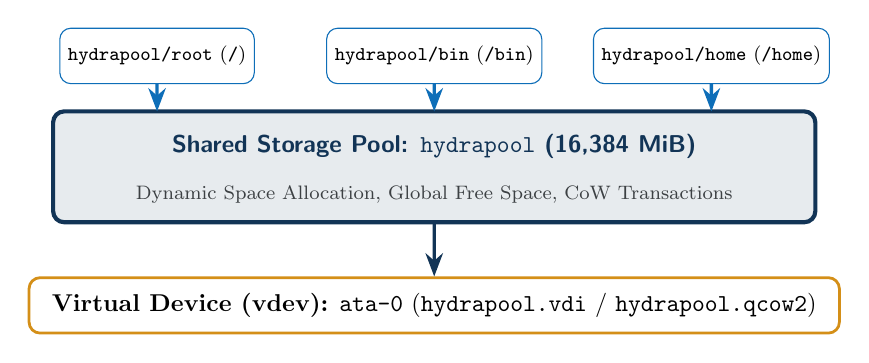
\begin{tikzpicture}[scale=0.88, every node/.style={transform shape}]
    % Datasets
    \node[draw=rustkeyword, fill=white, rounded corners, minimum width=2.5cm, minimum height=0.8cm] (ds1) at (0, 4) {\footnotesize \texttt{hydrapool/root} (\texttt{/})};
    \node[draw=rustkeyword, fill=white, rounded corners, minimum width=2.5cm, minimum height=0.8cm] (ds2) at (4, 4) {\footnotesize \texttt{hydrapool/bin} (\texttt{/bin})};
    \node[draw=rustkeyword, fill=white, rounded corners, minimum width=2.5cm, minimum height=0.8cm] (ds3) at (8, 4) {\footnotesize \texttt{hydrapool/home} (\texttt{/home})};

    % The Pool
    \draw[fill=hydrablue!10, draw=hydrablue, line width=1.5pt, rounded corners] (-1.5, 1.6) rectangle (9.5, 3.2);
    \node[font=\bfseries\sffamily\color{hydrablue}] at (4, 2.7) {Shared Storage Pool: \texttt{hydrapool} (16,384 MiB)};
    \node[font=\footnotesize\color{hydragray}] at (4, 2.0) {Dynamic Space Allocation, Global Free Space, CoW Transactions};

    % Hardware VDEV
    \node[draw=hydragold, fill=white, rounded corners, line width=1pt, minimum width=6cm, minimum height=0.8cm] (vdev) at (4, 0.4) {
        \begin{tabular}{c}
            \textbf{Virtual Device (vdev):} \texttt{ata-0} (\texttt{hydrapool.vdi} / \texttt{hydrapool.qcow2})
        \end{tabular}
    };

    \draw[->, >=Stealth, line width=1.2pt, rustkeyword] (ds1) -- (0, 3.2);
    \draw[->, >=Stealth, line width=1.2pt, rustkeyword] (ds2) -- (4, 3.2);
    \draw[->, >=Stealth, line width=1.2pt, rustkeyword] (ds3) -- (8, 3.2);
    \draw[->, >=Stealth, line width=1.2pt, hydrablue] (4, 1.6) -- (vdev);
\end{tikzpicture}
\caption{The OpenZFS Pooled Storage Hierarchy in Hydra.}
\label{fig:zfs_hierarchy}
\end{figure}

\subsection{Virtual Devices (vdevs)}
A storage pool is constructed from a tree of **Virtual Devices (vdevs)**:
\begin{itemize}
    \item \textbf{Leaf vdevs:} Physical disks, partitions, or virtual disk image files (e.g., \texttt{hydrapool.vdi}).
    \item \textbf{Interior vdevs:} RAID topologies:
    \begin{itemize}
        \item \textbf{Mirror:} Mirrors data identically across two or more devices ($N$-way mirroring).
        \item \textbf{RAID-Z1, RAID-Z2, RAID-Z3:} Parity-based distributed striping tolerant of 1, 2, or 3 concurrent disk failures.
    \end{itemize}
\end{itemize}

All datasets created within a pool draw dynamically from its common free space. There are no fixed partition sizes; if \texttt{hydrapool} has 10~GB of unallocated space, every dataset can draw from that space on demand.

% ==============================================================================
\section{The Uberblock Ring and Transaction Groups (TXGs)}
\label{sec:uberblock_ring}
% ==============================================================================

In ZFS, the fundamental root of trust on physical media is the \textbf{Uberblock}. The uberblock identifies the current transaction group number (\texttt{txg}), the physical location of the space maps, and the root dnode pointing to the Master Node Object.

To prevent write failures from corrupting the uberblock, ZFS reserves blocks 1 through 32 of each vdev as an **Uberblock Ring**:
\begin{equation}
\text{Uberblock Slot Index} = \text{TXG} \pmod{32}
\end{equation}

When Hydra boots, the ZFS server scans all 32 slots, validates each slot's checksum, and selects the uberblock with the highest valid \texttt{TXG} number.

\begin{lstlisting}[language=Rust, caption={Scanning the Uberblock Ring in Hydra (\texttt{src/fs/zfs/mod.rs})}]
let mut best_uberblock: Option<Uberblock> = None;
for slot in 0..32 {
    let block_offset = (1 + slot) * BLOCK_SIZE;
    let raw_bytes = ata_driver.read_block(block_offset)?;
    if let Ok(ub) = Uberblock::decode(&raw_bytes) {
        if ub.magic == UBERBLOCK_MAGIC && ub.verify_checksum() {
            if best_uberblock.as_ref().map_or(true, |best| ub.txg > best.txg) {
                best_uberblock = Some(ub);
            }
        }
    }
}
\end{lstlisting}

% ==============================================================================
\section{Copy-on-Write (CoW) and Merkle Tree Self-Healing}
\label{sec:cow_merkle}
% ==============================================================================

ZFS never overwrites existing data blocks in place. When a write occurs:
\begin{enumerate}
    \item A new physical block is allocated from the free space bitmap.
    \item The modified data is written to the new block.
    \item The parent indirect block is updated to point to the new block, and its own cryptographic checksum (Fletcher-4 or SHA-256) is recalculated.
    \item This bubbling-up process continues all the way to the top of the tree, culminating in writing a new Uberblock in the next slot of the Uberblock Ring.
\end{enumerate}

\begin{figure}[htbp]
\centering
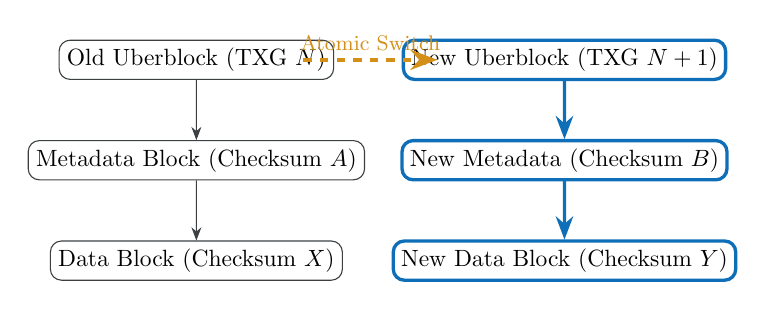
\begin{tikzpicture}[scale=0.85, every node/.style={transform shape}]
    % Old tree
    \node[draw=hydragray, fill=white, rounded corners] (ub_old) at (2, 5) {Old Uberblock (TXG $N$)};
    \node[draw=hydragray, fill=white, rounded corners] (meta_old) at (2, 3.5) {Metadata Block (Checksum $A$)};
    \node[draw=hydragray, fill=white, rounded corners] (data_old) at (2, 2) {Data Block (Checksum $X$)};
    \draw[->, >=Stealth, hydragray] (ub_old) -- (meta_old);
    \draw[->, >=Stealth, hydragray] (meta_old) -- (data_old);

    % New tree
    \node[draw=rustkeyword, fill=white, line width=1.2pt, rounded corners] (ub_new) at (7.5, 5) {New Uberblock (TXG $N+1$)};
    \node[draw=rustkeyword, fill=white, line width=1.2pt, rounded corners] (meta_new) at (7.5, 3.5) {New Metadata (Checksum $B$)};
    \node[draw=rustkeyword, fill=white, line width=1.2pt, rounded corners] (data_new) at (7.5, 2) {New Data Block (Checksum $Y$)};
    \draw[->, >=Stealth, line width=1.2pt, rustkeyword] (ub_new) -- (meta_new);
    \draw[->, >=Stealth, line width=1.2pt, rustkeyword] (meta_new) -- (data_new);

    % Arrow indicating transition
    \draw[->, >=Stealth, dashed, line width=1.5pt, hydragold] (3.6, 5) -- node[above] {\small Atomic Switch} (5.6, 5);
\end{tikzpicture}
\caption{Copy-on-Write (CoW) State Transition in ZFS.}
\label{fig:zfs_cow}
\end{figure}

Because the new tree is completely written to disk before the new uberblock is committed, **ZFS is crash-consistent by design**. A power outage mid-transaction simply abandons the partially written unreferenced blocks; on reboot, the system safely mounts the previous valid TXG without corruption.

\subsection{The Fletcher-4 Checksum Algorithm}
Every block pointer in ZFS contains a 256-bit cryptographic or mathematical checksum of the block it references. The primary algorithm used for high performance in Hydra is **Fletcher-4**:

\begin{equation}
\begin{aligned}
A &= \sum_{i=1}^{N} D_i \pmod{2^{64}} \\
B &= \sum_{i=1}^{N} A_i \pmod{2^{64}} \\
C &= \sum_{i=1}^{N} B_i \pmod{2^{64}} \\
D &= \sum_{i=1}^{N} C_i \pmod{2^{64}}
\end{aligned}
\end{equation}

When reading a block from disk, the ZFS server recalculates Fletcher-4 across the 4096 bytes and compares it to the 256-bit hash stored in the parent block pointer. If a discrepancy is detected (silent data corruption), ZFS refuses to return corrupt data to user space. If redundant mirrors or RAID-Z vdevs are present, ZFS automatically fetches the uncorrupted copy from another device, repairs the corrupted sector on disk, and returns clean data---a feature known as **Self-Healing Storage**.

% ==============================================================================
\section{Dnodes and the ZFS POSIX Layer (ZPL)}
\label{sec:dnodes}
% ==============================================================================

In ZFS, every file, directory, and dataset is represented by a **dnode** (the ZFS equivalent of an inode). A standard dnode occupies 512 bytes:

\begin{lstlisting}[language=Rust, caption={ZFS Dnode Structure in Hydra (\texttt{src/fs/zfs/types.rs})}]
#[repr(C)]
pub struct DNodePhys {
    pub dnode_type: u8,        // DMU object type (e.g., ZPL_FILE, ZPL_DIR)
    pub indblkshift: u8,       // Indirect block shift
    pub nlevels: u8,           // Indirection depth (0 = direct blocks)
    pub nblkptr: u8,           // Number of direct block pointers
    pub bonus_type: u8,        // Bonus buffer type
    pub checksum: u8,          // Checksum algorithm (Fletcher-4)
    pub compress: u8,          // Compression type (LZ4 / ZSTD / Off)
    pub flags: u8,             // Dnode flags
    pub data_blk_size_sec: u16,// Data block size in sectors
    pub max_blkid: u64,        // Highest logical block ID
    pub blkptr: [BlockPointer; 3], // Direct block pointers
    pub bonus: [u8; 320],      // Bonus buffer: POSIX mode, UID, GID, size
}
\end{lstlisting}

\subsection{The ZFS Attribute Processor (ZAP)}
To store directory entries and extended attributes (xattrs), ZFS implements the **ZFS Attribute Processor (ZAP)**:
\begin{itemize}
    \item \textbf{Micro-ZAP:} For small directories containing fewer than a few dozen files, entries are packed into a single 4096-byte leaf block using an array of name-value pairs.
    \item \textbf{Fat-ZAP:} When directories scale to thousands of files, ZAP promotes the object to an on-disk hash table indexed by a 64-bit hash of the filename, ensuring $O(1)$ lookup performance regardless of directory size.
\end{itemize}

% ==============================================================================
\section{The Microkernel Storage Server Hierarchy}
\label{sec:storage_server}
% ==============================================================================

In accordance with microkernel design principles, Hydra divides the storage subsystem into three strictly segregated layers:

\begin{table}[htbp]
\centering
\small
\begin{tabular}{llll}
\hline
\textbf{Component} & \textbf{Ring Mode} & \textbf{Endpoint} & \textbf{Primary Responsibility} \\
\hline
\texttt{ata\_driver} & Ring 3 Process & \texttt{0x21} & ATA controller registers, Bus-Master DMA, PRD tables \\
\texttt{zfs\_server} & Ring 3 Process & \texttt{0x20} & TXG management, space maps, dnode walks, Fletcher-4 \\
\texttt{ZfsClient} / VFS & Kernel / Lib & N/A & Path resolution, file descriptors, POSIX syscall shims \\
\hline
\end{tabular}
\caption{The Three-Tier Storage Server Hierarchy in Hydra.}
\label{tab:storage_layers}
\end{table}

When an application calls \texttt{read(fd, buf, count)}, the request passes through \texttt{ZfsClient}, which transmits a structured request over IPC Endpoint \texttt{0x20} to \texttt{zfs\_server}. If the requested dnode block is not cached in RAM, \texttt{zfs\_server} sends an IPC sector read request over Endpoint \texttt{0x21} to \texttt{ata\_driver}, which programs the PCI bus-master DMA controller to stream raw disk sectors into physical memory.

% ==============================================================================
\section{Summary}
\label{sec:summary_chap4}
% ==============================================================================

Hydra’s adoption of OpenZFS represents a qualitative leap over classic educational operating system file systems:
\begin{itemize}
    \item Pooled storage unifies physical devices and eliminates static partition boundaries.
    \item The 32-slot Uberblock Ring and Copy-on-Write transaction model provide mathematical crash-resilience without the overhead of write-ahead logging.
    \item Fletcher-4 checksumming embedded in block pointers forms a Merkle tree that guarantees detection and isolation of silent data corruption.
    \item Separating raw disk I/O (\texttt{ata\_driver}) from file system logic (\texttt{zfs\_server}) maintains the microkernel principle of least privilege.
\end{itemize}

% ==============================================================================
\section{Exercises and Review Problems}
\label{sec:exercises_chap4}
% ==============================================================================

\begin{enumerate}
    \item \textbf{File System Integrity:} Why is \texttt{fsck} inherently incapable of detecting silent data corruption (bit rot)? How does OpenZFS solve this problem?
    \item \textbf{Copy-on-Write Mechanics:} Diagram the exact sequence of block writes that occur when modifying a single byte inside a 100~MiB file in ZFS. Why does the top-level Uberblock have to be updated last?
    \item \textbf{Uberblock Ring Math:} Why does ZFS maintain a 32-slot ring of uberblocks rather than simply updating a single fixed uberblock at sector 0? What mathematical formula determines the slot index of transaction group $N$?
    \item \textbf{Fletcher-4 Math:} Compute the four 64-bit accumulators ($A, B, C, D$) of the Fletcher-4 checksum algorithm for a simple four-word data sequence $[1, 2, 3, 4]$.
    \item \textbf{Merkle Trees:} Explain how embedding the checksum of a child block inside its parent block pointer prevents malicious spoofing of disk blocks.
    \item \textbf{Dnodes vs. Inodes:} Contrast the 512-byte ZFS \texttt{DNodePhys} structure with a classic 128-byte UNIX ext2 inode. What purpose is served by the 320-byte bonus buffer?
    \item \textbf{Directory Hashing:} Describe the difference between a Micro-ZAP and a Fat-ZAP. Why is a hash-table directory structure preferable to a linear array when a directory contains 100,000 files?
    \item \textbf{Microkernel Separation:} Suppose the Ring~3 \texttt{ata\_driver} process crashes while servicing a disk request. How does the microkernel supervisor recover the system without losing data or crashing the \texttt{zfs\_server}?
    \item \textbf{Write Amplification:} Compare the write amplification of a journaling file system (ext4 with data journaling) versus a Copy-on-Write file system (ZFS) during heavy random write workloads.
    \item \textbf{Design Problem:} Design an atomic snapshot mechanism for OpenZFS. How does the Copy-on-Write tree structure allow a snapshot of a 10~Terabyte file system to be created instantaneously in zero seconds without copying data?
\end{enumerate}

\chapter{Input/Output and Device Drivers}
\label{chap:io}

The central processing unit and main memory exist to execute computations, but a computer isolated from the external world is fundamentally sterile. The \textbf{Input/Output (I/O)} subsystem bridges the computational core to the physical world: receiving keystrokes and mouse motions, streaming megabytes of disk blocks, transmitting packets across fiber-optic networks, and driving high-resolution graphical displays.

In traditional operating systems, authoring device drivers is notorious for being the most error-prone domain in software engineering. Device drivers must directly program physical hardware registers, configure asynchronous direct memory access (DMA) transfers, and service hardware interrupt requests (IRQs). A single pointer mistake or race condition in a Ring~0 driver brings down the entire operating system.

In this chapter, we explore the principles of I/O hardware and software, examine disk scheduling and DMA architectures, and analyze how Hydra achieves **true Ring~3 driver isolation** using hardware I/O Permission Bitmaps and asynchronous interrupt forwarding.

% ==============================================================================
\section{Principles of I/O Hardware}
\label{sec:io_hardware}
% ==============================================================================

I/O devices span an enormous range of data rates and operational characteristics, from a keyboard producing 10 bytes per second to an NVMe drive or 100-Gigabit Ethernet NIC transferring billions of bytes per second.

\subsection{Device Controllers and Interfaces}
An I/O unit typically consists of two distinct components:
\begin{enumerate}
    \item \textbf{The Mechanical / Physical Device:} The physical disk platters, flash memory dies, LCD pixel arrays, or copper Ethernet transceivers.
    \item \textbf{The Electronic Controller (Device Controller / Chipset):} A specialized integrated circuit (often featuring its own microcontroller, firmware, and local SRAM) that manages the device's physical signals and exposes a standardized programming interface to the system bus.
\end{enumerate}

The interface between the controller and the CPU consists of a set of **Registers**:
\begin{itemize}
    \item \textbf{Command Register:} Software writes commands (e.g., READ, WRITE, SEEK, RESET) to instruct the controller what operation to perform.
    \item \textbf{Status Register:} Software reads status bitflags (e.g., READY, BUSY, ERROR, DATA\_REQUEST) to monitor device state.
    \item \textbf{Data In / Data Out Registers:} Buffers through which bytes are transferred into or out of the controller.
\end{itemize}

\subsection{Port-Mapped I/O vs. Memory-Mapped I/O}
Modern processors communicate with controller registers using two fundamentally different hardware architectures:

\begin{figure}[htbp]
\centering
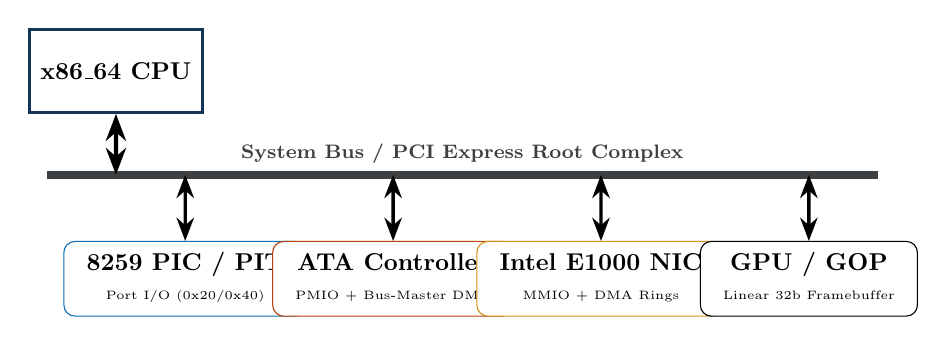
\begin{tikzpicture}[scale=0.88, every node/.style={transform shape}]
    % CPU
    \node[draw=hydrablue, fill=white, line width=1.2pt, minimum width=2.5cm, minimum height=1.2cm] (cpu) at (0, 3) {\textbf{x86\_64 CPU}};

    % Bus
    \draw[line width=3pt, hydragray] (-1, 1.5) -- (11, 1.5);
    \node[font=\footnotesize\bfseries\color{hydragray}] at (5, 1.8) {System Bus / PCI Express Root Complex};

    % Devices
    \node[draw=rustkeyword, fill=white, rounded corners, minimum width=2.2cm, minimum height=1cm] (pic) at (1, 0) {
        \begin{tabular}{c}
            \textbf{8259 PIC / PIT}\\
            \tiny Port I/O (0x20/0x40)
        \end{tabular}
    };
    \node[draw=rustred, fill=white, rounded corners, minimum width=2.2cm, minimum height=1cm] (ata) at (4, 0) {
        \begin{tabular}{c}
            \textbf{ATA Controller}\\
            \tiny PMIO + Bus-Master DMA
        \end{tabular}
    };
    \node[draw=hydragold, fill=white, rounded corners, minimum width=2.2cm, minimum height=1cm] (e1000) at (7, 0) {
        \begin{tabular}{c}
            \textbf{Intel E1000 NIC}\\
            \tiny MMIO + DMA Rings
        \end{tabular}
    };
    \node[draw=black, fill=white, rounded corners, minimum width=2.2cm, minimum height=1cm] (gpu) at (10, 0) {
        \begin{tabular}{c}
            \textbf{GPU / GOP}\\
            \tiny Linear 32b Framebuffer
        \end{tabular}
    };

    \draw[<->, >=Stealth, line width=1.5pt] (cpu) -- (0, 1.5);
    \draw[<->, >=Stealth, line width=1.2pt] (pic) -- (1, 1.5);
    \draw[<->, >=Stealth, line width=1.2pt] (ata) -- (4, 1.5);
    \draw[<->, >=Stealth, line width=1.2pt] (e1000) -- (7, 1.5);
    \draw[<->, >=Stealth, line width=1.2pt] (gpu) -- (10, 1.5);
\end{tikzpicture}
\caption{System Interconnects: Port I/O, MMIO, and DMA across the PCI Bus.}
\label{fig:pci_bus}
\end{figure}

\begin{enumerate}
    \item \textbf{Port-Mapped I/O (PMIO):} The processor implements an independent 16-bit I/O address space ($0\text{x}0000$ to $0\text{xFFFF}$) physically separate from main memory. Reading and writing require special assembly instructions:
    \begin{itemize}
        \item \texttt{inb \%dx, \%al}: Reads one byte from I/O port \texttt{DX} into register \texttt{AL}.
        \item \texttt{outb \%al, \%dx}: Writes one byte from register \texttt{AL} to I/O port \texttt{DX}.
    \end{itemize}
    Legacy PC hardware (the 8259 PIC, 8254 PIT, 16550 serial UART, and standard IDE/ATA hard disk controllers) communicates via PMIO.
    \item \textbf{Memory-Mapped I/O (MMIO):} Device controller registers are mapped directly into the CPU's physical memory address space.
    \begin{itemize}
        \item A driver reads a hardware register using standard pointer dereferences (e.g., \texttt{*ptr} in Rust or \texttt{mov (\%rdi), \%rax} in assembly).
        \item \textit{Crucial Requirement:} Because writing to an MMIO register causes immediate physical side effects (such as transmitting an Ethernet packet or resetting a controller), the operating system \textbf{must mark the corresponding page table entry with \texttt{NO\_CACHE}} (Page Table bit 4 set). If caching were enabled, the CPU cache controller would swallow the write or return stale data without touching the physical device!
    \end{itemize}
\end{enumerate}

% ==============================================================================
\section{Direct Memory Access (DMA) and Scatter-Gather PRDs}
\label{sec:dma_deep}
% ==============================================================================

If the central processor had to execute an \texttt{in} instruction for every 16-bit word read from a storage controller or network interface, streaming a 10~GiB file would consume 100\% of the CPU's processing capacity.

\subsection{Programmed I/O vs. DMA}
Operating systems transfer data using three sequential paradigms:
\begin{enumerate}
    \item \textbf{Programmed I/O (Polling):} The CPU polls the controller's status register in a busy-wait loop until the device announces that data is ready, then executes a loop of \texttt{in} instructions to transfer bytes into memory. This monopolizes the CPU.
    \item \textbf{Interrupt-Driven I/O:} The CPU issues a command to the controller and switches to another thread. When the controller fills an internal buffer, it asserts a hardware interrupt. The CPU traps into the kernel, copies the data, and returns. While better than polling, the CPU still handles every byte.
    \item \textbf{Direct Memory Access (DMA):} The CPU instructs the controller to act as a **Bus Master**. The device controller reads or writes data directly across the system bus into physical DRAM without passing through CPU registers.
\end{enumerate}

\subsection{Physical Region Descriptors (PRDs) and Scatter-Gather}
In modern virtual memory operating systems, a contiguous 64~KiB user-space buffer is rarely contiguous in physical RAM: it may be composed of 16 distinct 4096-byte physical frames scattered across memory.

To accommodate this, modern DMA controllers support **Scatter-Gather DMA**. The driver constructs a table of **Physical Region Descriptors (PRD Table)** in physical memory:

\begin{figure}[htbp]
\centering
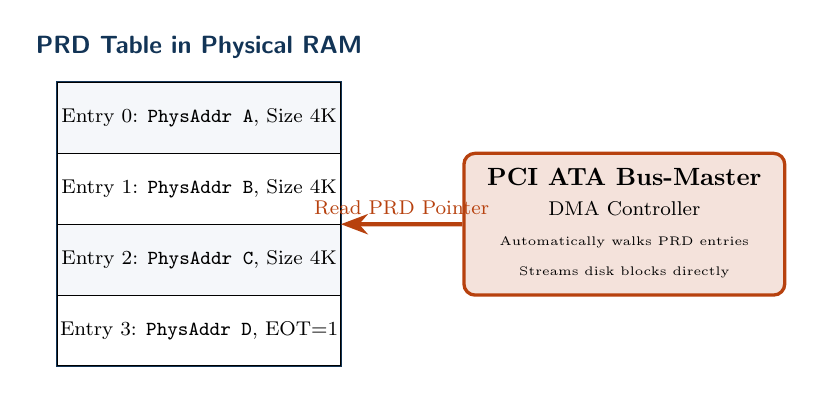
\begin{tikzpicture}[scale=0.9, every node/.style={transform shape}]
    % PRD Table
    \node[font=\bfseries\sffamily\color{hydrablue}] at (2, 4.5) {PRD Table in Physical RAM};
    \draw[fill=white, draw=hydrablue, line width=1pt] (0, 0) rectangle (4, 4);
    
    \draw[fill=hydralight] (0, 3) rectangle (4, 4);
    \node at (2, 3.5) {\footnotesize Entry 0: \texttt{PhysAddr A}, Size 4K};
    
    \draw[fill=white] (0, 2) rectangle (4, 3);
    \node at (2, 2.5) {\footnotesize Entry 1: \texttt{PhysAddr B}, Size 4K};
    
    \draw[fill=hydralight] (0, 1) rectangle (4, 2);
    \node at (2, 1.5) {\footnotesize Entry 2: \texttt{PhysAddr C}, Size 4K};
    
    \draw[fill=white] (0, 0) rectangle (4, 1);
    \node at (2, 0.5) {\footnotesize Entry 3: \texttt{PhysAddr D}, EOT=1};

    % ATA Controller
    \node[draw=rustred, fill=rustred!15, line width=1.2pt, rounded corners, minimum width=3.5cm, minimum height=2cm] (ata) at (8, 2) {
        \begin{tabular}{c}
            \textbf{PCI ATA Bus-Master}\\
            \footnotesize DMA Controller\\
            \tiny Automatically walks PRD entries\\
            \tiny Streams disk blocks directly
        \end{tabular}
    };

    \draw[->, >=Stealth, line width=1.5pt, rustred] (ata) -- node[above] {\footnotesize Read PRD Pointer} (4, 2);
\end{tikzpicture}
\caption{Scatter-Gather DMA using Physical Region Descriptor (PRD) Tables.}
\label{fig:dma_prd}
\end{figure}

Each 8-byte PRD entry specifies:
\begin{itemize}
    \item A 32-bit physical base address of a RAM frame;
    \item A 16-bit byte count;
    \item An End-Of-Table (\texttt{EOT}) bit indicating the final descriptor.
\end{itemize}

In Hydra's Ring~3 ATA driver (\texttt{userland/drivers/ata-driver/src/main.rs}), the driver builds this PRD table directly from the physical frame addresses allocated to the OpenZFS storage pool, commands the controller to initiate Bus-Master DMA, and suspends execution until the hardware raises IRQ~14.

% ==============================================================================
\section{Microkernel Driver Isolation in Ring~3}
\label{sec:driver_isolation_deep}
% ==============================================================================

In a monolithic operating system like Linux, device drivers execute in Ring~0. If an audio or Wi-Fi driver attempts to write to a null pointer, the processor generates a Page Fault in kernel mode, precipitating an unrecoverable kernel panic.

Hydra enforces **strict driver containment**: all device drivers execute exclusively as isolated Ring~3 user-space processes.

\subsection{The x86 I/O Permission Bitmap (IOPB)}
How can an unprivileged Ring~3 process execute \texttt{in} and \texttt{out} instructions on disk controller ports without granting it general kernel authority?

The x86 architecture provides the **I/O Permission Bitmap (IOPB)** within the Task State Segment (TSS):
\begin{enumerate}
    \item The IOPB is an 8192-byte bitmask ($65,536\text{ bits}$) stored at the end of the TSS.
    \item Each bit corresponds to one of the 65,536 I/O ports.
    \item When a Ring~3 thread executes an \texttt{in} or \texttt{out} instruction, the CPU checks the corresponding bit in the IOPB:
    \begin{itemize}
        \item If the bit is \texttt{0}, the instruction executes successfully at full hardware speed.
        \item If the bit is \texttt{1}, the CPU generates an immediate General Protection Fault (\texttt{\#GP}, Exception 13), terminating the unauthorized operation.
    \end{itemize}
\end{enumerate}

Hydra's supervisor configures the IOPB with surgical precision:
\begin{itemize}
    \item \texttt{ata\_driver} (Process 2) is granted access \textbf{only} to the ATA command and control ports (\texttt{0x1F0}--\texttt{0x1F7}, \texttt{0x3F6}) and Bus-Master DMA registers.
    \item \texttt{display\_server} (Process 5) is granted access \textbf{only} to the Bochs/VGA frame control ports.
    \item If the disk driver attempts to touch the keyboard controller (port \texttt{0x60}) or reprogram the system timer (port \texttt{0x40}), it is halted immediately by the hardware MMU.
\end{itemize}

% ==============================================================================
\section{Hardware Interrupts to IPC Notifications}
\label{sec:interrupt_dispatch_deep}
% ==============================================================================

When a disk controller completes a DMA transfer or a network card receives an Ethernet frame, the hardware asserts an electrical Interrupt Request (IRQ) line. The CPU interrupts the currently executing thread and traps into the Ring~0 IDT handler.

In a microkernel, driver logic cannot be executed inside the Ring~0 interrupt handler. Hydra implements an asynchronous **Interrupt-to-IPC Forwarding Pipeline**:

\begin{figure}[htbp]
\centering
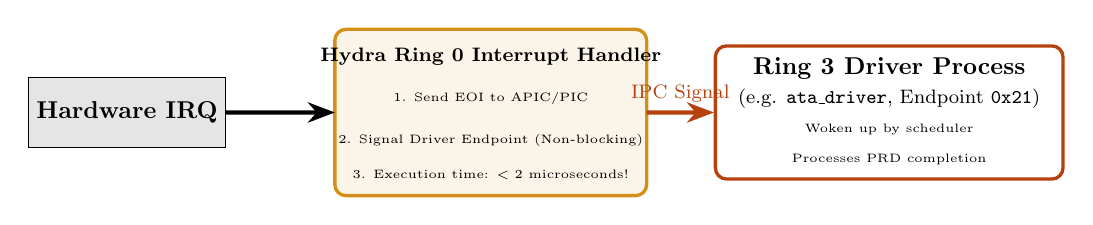
\begin{tikzpicture}[scale=0.88, every node/.style={transform shape}]
    % Hardware
    \node[draw=black, fill=gray!20, minimum width=2.5cm, minimum height=1cm] (hw) at (0, 3) {\textbf{Hardware IRQ}};
    
    % Ring 0
    \draw[fill=hydragold!10, draw=hydragold, line width=1.2pt, rounded corners] (3, 1.8) rectangle (7.5, 4.2);
    \node[font=\bfseries\footnotesize\color{black}] at (5.25, 3.8) {Hydra Ring 0 Interrupt Handler};
    \node[font=\tiny] at (5.25, 3.2) {1. Send EOI to APIC/PIC};
    \node[font=\tiny] at (5.25, 2.6) {2. Signal Driver Endpoint (Non-blocking)};
    \node[font=\tiny] at (5.25, 2.1) {3. Execution time: $< 2$ microseconds!};

    % Ring 3 Driver
    \node[draw=rustred, fill=white, line width=1.2pt, rounded corners, minimum width=3.5cm, minimum height=1.5cm] (drv) at (11, 3) {
        \begin{tabular}{c}
            \textbf{Ring 3 Driver Process}\\
            \footnotesize (e.g. \texttt{ata\_driver}, Endpoint \texttt{0x21})\\
            \tiny Woken up by scheduler\\
            \tiny Processes PRD completion
        \end{tabular}
    };

    \draw[->, >=Stealth, line width=1.5pt] (hw) -- (3, 3);
    \draw[->, >=Stealth, line width=1.5pt, rustred] (7.5, 3) -- node[above] {\footnotesize IPC Signal} (drv);
\end{tikzpicture}
\caption{The Hardware Interrupt to Ring~3 IPC Notification Pipeline.}
\label{fig:irq_pipeline}
\end{figure}

\begin{lstlisting}[language=Rust, caption={Converting Hardware IRQs to IPC Signals (\texttt{src/arch/idt.rs})}]
pub fn dispatch_irq(irq: u8) {
    // Acknowledge hardware interrupt controller immediately
    pic::send_eoi(irq);

    // Forward as lightweight IPC signal to registered driver endpoint
    match irq {
        1  => input::enqueue_keyboard_scancode(read_port(0x60)),
        14 => ipc::notify_endpoint(EndpointId(0x21), SIGNAL_DMA_COMPLETE),
        11 => ipc::notify_endpoint(EndpointId(0x22), SIGNAL_PACKET_ARRIVED),
        _  => {}
    }
}
\end{lstlisting}

This architecture achieves two profound advantages:
\begin{enumerate}
    \item \textbf{Minimal Interrupt Latency:} The Ring~0 handler does no work beyond sending an End-of-Interrupt (EOI) and posting a bit flag to an IPC endpoint, completing in fewer than 200 clock cycles.
    \item \textbf{Immunity to Driver Freezes:} If a driver enters an infinite loop while processing data, it does not lock the CPU's interrupt system. The preemptive scheduler simply expires the driver's timeslice and continues running user applications!
\end{enumerate}

% ==============================================================================
\section{The Graphics Subsystem: DRM, KMS, and Wayland}
\label{sec:graphics_subsystem}
% ==============================================================================

Modern graphical operating systems have abandoned legacy VGA text modes. Modern displays operate at resolutions of $1920\times1080$, $2560\times1440$, or $3840\times2160$ pixels in 32-bit True Color (ARGB8888).

\subsection{UEFI Graphics Output Protocol (GOP)}
During boot, Hydra queries the UEFI firmware's Graphics Output Protocol (GOP). GOP configures the motherboard display controller and returns:
\begin{itemize}
    \item A 64-bit physical base address of the linear framebuffer;
    \item Horizontal and vertical resolution (e.g., $1024\times768$);
    \item Pixels per scanline (pitch);
    \item Pixel format (typically \texttt{PixelBlueGreenRedReserved8BitPerColor}).
\end{itemize}

Hydra maps this physical framebuffer into the address space of the Ring~3 \texttt{display\_server} process (\texttt{userland/drivers/display-server/}).

\subsection{Linux DRM/KMS Emulation and Double-Buffering}
To allow unmodified modern graphical desktop environments (such as the **KWin Wayland compositor** and **KDE Plasma 6**) to run on Hydra, the kernel exposes a Linux-compatible **Direct Rendering Manager (DRM)** and **Kernel Mode Setting (KMS)** character device node at \texttt{/dev/dri/card0}:
\begin{itemize}
    \item \texttt{DRM\_IOCTL\_MODE\_GETRESOURCES}: Reports connected connectors, encoders, and CRTCs.
    \item \texttt{DRM\_IOCTL\_MODE\_CREATE\_DUMB}: Allocates a linear off-screen drawing surface in shared memory.
    \item \textbf{Atomic Page Flipping (\texttt{DRM\_IOCTL\_MODE\_PAGE\_FLIP}):} KWin renders desktop windows into an off-screen surface. When the frame is complete, it issues an atomic page-flip ioctl. The display server swaps the display pointer during the vertical blanking interval (VBLANK), delivering tear-free, 60~FPS graphics.
\end{itemize}

% ==============================================================================
\section{Summary}
\label{sec:summary_chap5}
% ==============================================================================

Input/Output systems connect computational hardware to external reality through Port I/O (PMIO), Memory-Mapped I/O (MMIO), and high-speed Bus-Master DMA. Traditional monolithic operating systems suffer from catastrophic instability because device drivers execute in Ring~0 with full supervisor authority.

Hydra solves this reliability crisis by isolating device drivers inside Ring~3 user-space processes. Hardware port access is confined through the x86 I/O Permission Bitmap (IOPB), while hardware interrupt requests are converted into non-blocking IPC notifications. Finally, high-performance display architectures leverage UEFI GOP linear buffers and DRM/KMS double-buffering to host modern Wayland and KDE Plasma desktops.

% ==============================================================================
\section{Exercises and Review Problems}
\label{sec:exercises_chap5}
% ==============================================================================

\begin{enumerate}
    \item \textbf{PMIO vs. MMIO:} Compare Port-Mapped I/O and Memory-Mapped I/O. Why must the page table entry for an MMIO aperture always have the \texttt{NO\_CACHE} bit set?
    \item \textbf{DMA Overhead:} Suppose a disk controller transfers 64~KiB of data. How many CPU instructions are executed if the transfer is performed via Programmed I/O versus Bus-Master DMA?
    \item \textbf{Scatter-Gather Descriptors:} Why is Scatter-Gather DMA indispensable in an operating system that utilizes virtual memory paging?
    \item \textbf{IOPB Security:} How many bytes are required for a complete x86\_64 I/O Permission Bitmap? What happens if a Ring~3 application attempts to execute an \texttt{outb} instruction on a port whose corresponding IOPB bit is \texttt{1}?
    \item \textbf{Interrupt Handling Latency:} Why is executing extensive computational logic inside a hardware interrupt handler considered bad practice in operating systems design? How does Hydra's IPC notification model eliminate this problem?
    \item \textbf{End of Interrupt (EOI):} What is the purpose of sending an End-of-Interrupt (EOI) command to the 8259 PIC or APIC controller? What happens if a driver fails to send EOI after servicing an interrupt?
    \item \textbf{Driver Crash Recovery:} If the Ring~3 \texttt{ata\_driver} encounters an assertion failure and crashes, why does the rest of the operating system remain running? Detail the steps taken by the Hydra supervisor to restart the driver and resume pending I/O requests.
    \item \textbf{Disk Scheduling:} Consider a disk with 200 cylinders. Requests arrive for cylinders 98, 183, 37, 122, 14, 124, 65, and 67. The disk head is currently at cylinder 53. Calculate the total head movement in cylinders for First-Come First-Served (FCFS) and the Elevator (SCAN) algorithm.
    \item \textbf{DRM Dumb Buffers:} Explain the role of DRM dumb buffers in modern Wayland compositors. How does double-buffering eliminate visual screen tearing?
    \item \textbf{Design Problem:} Design a user-space driver framework for a PCI Express NVMe solid-state drive. How would your design configure MMIO submission and completion queues, manage DMA memory buffers, and service completion interrupts without compromising microkernel isolation?
\end{enumerate}

\chapter{The Network Subsystem}
\label{chap:networking}

When Andrew Tanenbaum authored the original editions of \textit{Operating Systems: Design and Implementation}, local area networks were an emerging academic curiosity, and the MINIX operating system possessed no built-in TCP/IP networking stack. Today, an operating system devoid of network capabilities is functionally inert. Web browsers, cloud repositories, remote shells, distributed file systems, and automated package managers depend continuously on high-throughput, low-latency, packet-switched networking.

Integrating an enterprise-grade networking stack into a microkernel presents demanding architectural requirements:
\begin{enumerate}
    \item \textbf{Line-Rate Throughput:} At Gigabit and 10-Gigabit speeds, over one million packets can cross the physical wire every second. Copying packet payloads through multiple kernel memory boundaries exhausts memory bus bandwidth and destroys cache locality.
    \item \textbf{Complex Protocol State Machines:} The Transmission Control Protocol (TCP) requires sophisticated sliding window flow control, retransmission timers, congestion control algorithms, and multi-state lifecycle management.
    \item \textbf{POSIX Socket Compatibility:} Modern application workloads (including web browsers like Brave and graphical environments like KDE Plasma) demand complete compatibility with the BSD Socket API and non-blocking event multiplexing via \texttt{epoll}.
\end{enumerate}

In this chapter, we dissect the layered network architecture, examine the physical operation of the Intel 82540EM Gigabit Ethernet controller, explore circular DMA descriptor rings, walk through the protocol pipeline (ARP, IPv4, ICMP, UDP, TCP, and DHCP), and analyze how Hydra powers high-concurrency desktop networking in an isolated Ring~3 driver process.

% ==============================================================================
\section{Layered Network Architectures: The End-to-End Principle}
\label{sec:net_layers}
% ==============================================================================

Computer networks are structured as hierarchies of layers, where each layer provides a well-defined service to the layer above while hiding the implementation details of the layer below.

\subsection{The OSI Model vs. the Internet Protocol Suite}
The theoretical Open Systems Interconnection (OSI) 7-layer model defines Physical, Data Link, Network, Transport, Session, Presentation, and Application layers. In modern operating systems, the pragmatic 4-layer Internet Protocol suite (TCP/IP) is universally adopted:

\begin{figure}[htbp]
\centering
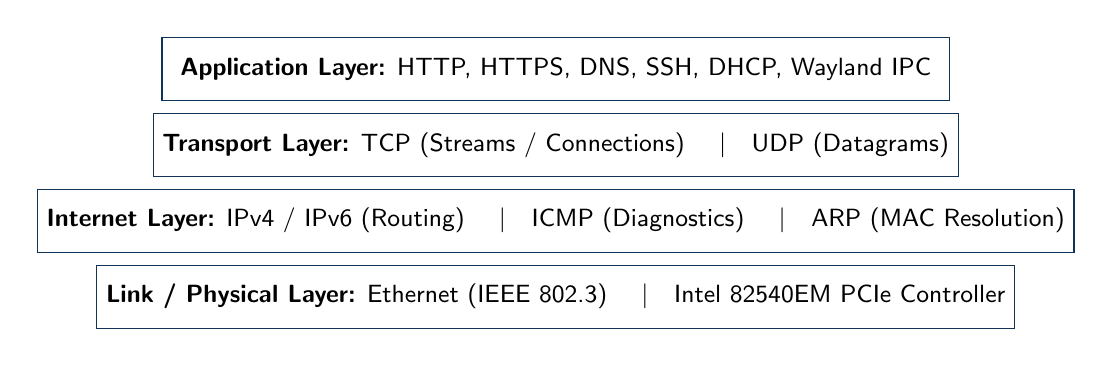
\begin{tikzpicture}[scale=0.9, every node/.style={transform shape}]
    \matrix (stack) [matrix of nodes, nodes={draw=hydrablue, minimum width=10cm, minimum height=0.8cm, fill=white, font=\small\sffamily}, column sep=0mm, row sep=1.5mm] {
        \textbf{Application Layer:} HTTP, HTTPS, DNS, SSH, DHCP, Wayland IPC \\
        \textbf{Transport Layer:} TCP (Streams / Connections) \quad\textbar\quad UDP (Datagrams) \\
        \textbf{Internet Layer:} IPv4 / IPv6 (Routing) \quad\textbar\quad ICMP (Diagnostics) \quad\textbar\quad ARP (MAC Resolution) \\
        \textbf{Link / Physical Layer:} Ethernet (IEEE 802.3) \quad\textbar\quad Intel 82540EM PCIe Controller \\
    };
\end{tikzpicture}
\caption{The Layered Network Protocol Stack.}
\label{fig:net_layers}
\end{figure}

\subsection{Encapsulation and Decapsulation}
When an application transmits data (for example, a browser requesting an HTML page):
\begin{enumerate}
    \item The application deposits the HTTP request string (\texttt{"GET / HTTP/1.1"}) into a socket buffer.
    \item The \textbf{Transport Layer (TCP)} prepends a 20-byte TCP header containing source/destination port numbers, sequence numbers, and control flags, forming a \textbf{TCP Segment}.
    \item The \textbf{Internet Layer (IPv4)} prepends a 20-byte IPv4 header containing source/destination IP addresses, Time-to-Live (TTL), and protocol identifiers, forming an \textbf{IP Packet}.
    \item The \textbf{Link Layer (Ethernet)} prepends a 14-byte Ethernet header (Destination MAC, Source MAC, EtherType) and appends a 4-byte Cyclic Redundancy Check (CRC32), forming an \textbf{Ethernet Frame}.
    \item The physical network interface card (NIC) serializes the frame into electrical signals onto the wire.
\end{enumerate}

Upon arrival at the destination machine, the hardware and driver perform the reverse operation: stripping headers, verifying checksums, and delivering the raw payload to the listening user socket.

% ==============================================================================
\section{The Intel 82540EM (e1000) Network Controller}
\label{sec:e1000_hardware}
% ==============================================================================

Hydra targets the industry-standard **Intel 82540EM Gigabit Ethernet Controller**, supported natively on physical hardware and standard virtual machine hypervisors (VirtualBox, QEMU, VMware).

The e1000 controller connects to the processor via the PCI / PCI Express bus. It acts as an autonomous bus-master device capable of streaming data directly to and from physical RAM without CPU intervention.

\subsection{PCI Discovery and MMIO Register Aperture}
During boot, Hydra's PCI scanner enumerates the configuration space, matching Vendor ID \texttt{0x8086} (Intel) and Device ID \texttt{0x100E} (82540EM). The kernel reads Base Address Register 0 (\texttt{BAR0}), which specifies the physical base address of the controller's 128~KiB Memory-Mapped I/O (MMIO) register aperture.

Key controller registers include:
\begin{itemize}
    \item \textbf{\texttt{CTRL} (Offset \texttt{0x0000}):} Device Control register. Software writes bit 26 (\texttt{RST}) to perform a hardware master reset, and configures speed (1000 Mbps Full Duplex) and auto-negotiation.
    \item \textbf{\texttt{STATUS} (Offset \texttt{0x0008}):} Device Status register. Indicates link state (UP/DOWN) and transmission duplex.
    \item \textbf{\texttt{RCTL} (Offset \texttt{0x0100}):} Receive Control register. Enables the receiver (\texttt{EN}), configures receive buffer size (e.g., 2048 bytes), and strips Ethernet CRC.
    \item \textbf{\texttt{TCTL} (Offset \texttt{0x0400}):} Transmit Control register. Enables transmission (\texttt{EN}) and collision detection parameters.
    \item \textbf{\texttt{RAL} / \texttt{RAH} (Offset \texttt{0x5400}):} Receive Address Low and High registers. Stores the 48-bit physical Ethernet MAC address harvested from the card's non-volatile EEPROM.
\end{itemize}

% ==============================================================================
\section{Circular DMA Descriptor Rings}
\label{sec:dma_descriptor_rings}
% ==============================================================================

To sustain high-speed packet processing without interrupting the CPU on every individual frame, the e1000 utilizes circular **DMA Descriptor Rings** in physical memory:

\begin{figure}[htbp]
\centering
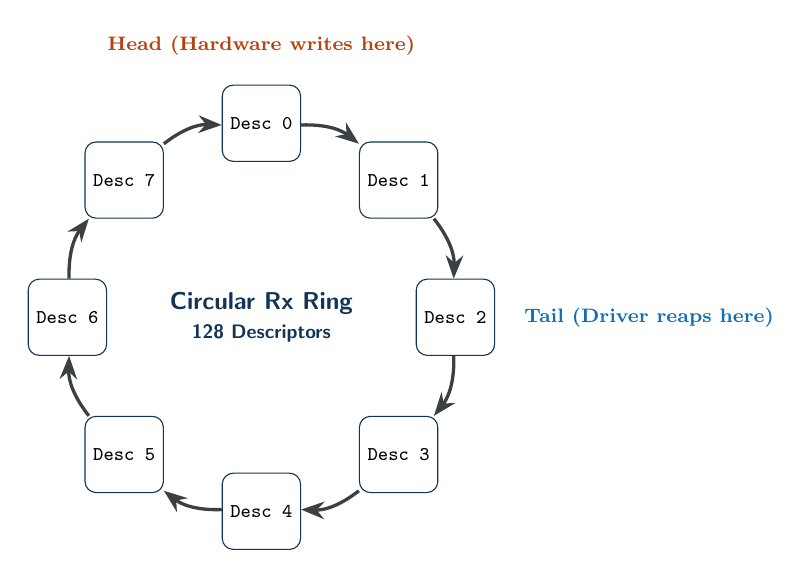
\begin{tikzpicture}[scale=0.88, every node/.style={transform shape}]
    % Circular ring represented as linked boxes
    \def\radius{2.8cm}
    \foreach \i in {0,...,7} {
        \node[draw=hydrablue, fill=white, rounded corners, minimum size=1.1cm] (desc\i) at ({-\i*45 + 90}:\radius) {\footnotesize \texttt{Desc \i}};
    }
    
    % Center label
    \node[align=center, font=\sffamily\bfseries\color{hydrablue}] at (0,0) {Circular Rx Ring\\ \footnotesize 128 Descriptors};

    % Arrows connecting circular ring
    \draw[->, >=Stealth, line width=1.2pt, hydragray] (desc0) to[bend left=20] (desc1);
    \draw[->, >=Stealth, line width=1.2pt, hydragray] (desc1) to[bend left=20] (desc2);
    \draw[->, >=Stealth, line width=1.2pt, hydragray] (desc2) to[bend left=20] (desc3);
    \draw[->, >=Stealth, line width=1.2pt, hydragray] (desc3) to[bend left=20] (desc4);
    \draw[->, >=Stealth, line width=1.2pt, hydragray] (desc4) to[bend left=20] (desc5);
    \draw[->, >=Stealth, line width=1.2pt, hydragray] (desc5) to[bend left=20] (desc6);
    \draw[->, >=Stealth, line width=1.2pt, hydragray] (desc6) to[bend left=20] (desc7);
    \draw[->, >=Stealth, line width=1.2pt, hydragray] (desc7) to[bend left=20] (desc0);

    % Pointers
    \node[above=0.3cm of desc0, font=\bfseries\footnotesize\color{rustred}] {Head (Hardware writes here)};
    \node[right=0.3cm of desc2, font=\bfseries\footnotesize\color{rustkeyword}] {Tail (Driver reaps here)};
\end{tikzpicture}
\caption{Circular DMA Descriptor Ring Architecture of the Intel E1000 Controller.}
\label{fig:e1000_ring}
\end{figure}

\subsection{The Receive (Rx) Descriptor Structure}
Hydra pre-allocates a circular array of 128 Receive Descriptors in non-swappable physical memory. Each descriptor is 16 bytes:

\begin{lstlisting}[language=Rust, caption={Intel E1000 Receive Descriptor (\texttt{src/net/e1000.rs})}]
#[repr(C)]
pub struct RxDescriptor {
    pub buffer_addr: u64, // Physical address of 2048-byte receive buffer
    pub length: u16,      // Length of received packet in bytes
    pub checksum: u16,    // Hardware-computed packet checksum
    pub status: u8,       // Descriptor status (Descriptor Done DD, End of Packet EOP)
    pub errors: u8,       // Hardware error flags (CRC error, symbol error)
    pub special: u16,     // VLAN tag
}
\end{lstlisting}

When an Ethernet frame arrives from the network:
\begin{enumerate}
    \item The card's DMA engine reads the descriptor pointed to by its internal \texttt{RDH} (Receive Descriptor Head) register.
    \item The hardware streams the packet bytes across the PCI bus directly into \texttt{buffer\_addr} in physical RAM.
    \item The hardware sets the \texttt{status} byte to indicate Descriptor Done (\texttt{DD}) and End-of-Packet (\texttt{EOP}), sets \texttt{length}, and increments the \texttt{RDH} pointer.
    \item The hardware asserts IRQ~11.
    \item Hydra's Ring~3 driver processes the packet from the buffer pointed to by \texttt{RDT} (Receive Descriptor Tail), resets the descriptor status, and advances \texttt{RDT}.
\end{enumerate}

Because packets are streamed directly into physical RAM mapped into the driver process, \textbf{zero memory copies are performed in the microkernel}!

% ==============================================================================
\section{The Network Protocol Pipeline}
\label{sec:protocol_pipeline_deep}
% ==============================================================================

Once a packet is harvested from the Rx descriptor ring, it enters Hydra's layered protocol pipeline (\texttt{src/net/stack.rs}):

\subsection{Ethernet Framing and the Address Resolution Protocol (ARP)}
At the link layer, packets are addressed via 48-bit Media Access Control (MAC) addresses (e.g., \texttt{08:00:27:41:47:51}). However, internet applications communicate using 32-bit IPv4 addresses (e.g., \texttt{10.0.2.15}).

The **Address Resolution Protocol (ARP)** maps IP addresses to physical MAC addresses:
\begin{itemize}
    \item When transmitting to an IP address on the local subnet whose MAC address is unknown, Hydra broadcasts an **ARP Request** frame to the broadcast MAC (\texttt{FF:FF:FF:FF:FF:FF}): \textit{"Who has 10.0.2.2? Tell 10.0.2.15"}.
    \item The target gateway node replies with an **ARP Reply** unicast packet: \textit{"10.0.2.2 is at 52:54:00:12:35:02"}.
    \item Hydra stores this mapping in its high-speed in-memory **ARP Cache**, with automatic timestamp expiration.
\end{itemize}

\subsection{The Internet Protocol (IPv4) and ICMP}
The IPv4 layer inspects incoming frames whose EtherType is \texttt{0x0800}:
\begin{enumerate}
    \item \textbf{Header Validation:} Verifies that the version is 4, header length is $\ge 20$ bytes, and the 16-bit Internet Header Checksum is mathematically valid.
    \item \textbf{Destination Verification:} Verifies that the destination IP matches the host's assigned IP (\texttt{10.0.2.15}) or the subnet broadcast address.
    \item \textbf{Protocol Demultiplexing:} Inspects the \texttt{protocol} byte:
    \begin{itemize}
        \item \texttt{0x01} (ICMP): Internet Control Message Protocol. Handles diagnostic \texttt{ECHO\_REQUEST} (ping) packets by immediately formulating an \texttt{ECHO\_REPLY} and returning it to the sender.
        \item \texttt{0x06} (TCP): Passes the payload to the Transmission Control Protocol engine.
        \item \texttt{0x11} (UDP): Passes the payload to the User Datagram Protocol engine.
    \end{itemize}
\end{enumerate}

\subsection{The User Datagram Protocol (UDP) and DNS Resolution}
UDP is a connectionless, lightweight transport protocol. Each UDP datagram contains an 8-byte header specifying Source Port, Destination Port, Length, and Checksum.

In Hydra, UDP powers domain name resolution:
\begin{itemize}
    \item When a user types a URL (e.g., \texttt{msn.com} or \texttt{google.com}) into the Brave web browser, the browser issues a standard DNS query to the nameserver (\texttt{10.0.2.3}) on UDP Port 53.
    \item Hydra transmits the datagram, records the query transaction ID, and suspends the calling thread on a socket wait queue.
    \item When the DNS response packet arrives over the wire, Hydra's socket demultiplexer matches the port, extracts the IP address record, and immediately awakens the browser thread.
\end{itemize}

\subsection{The Transmission Control Protocol (TCP) State Machine}
TCP provides a reliable, connection-oriented, full-duplex byte stream. It guarantees that bytes are delivered in order, without duplicates or loss, despite an unreliable underlying packet-switched network.

Hydra's TCP implementation (\texttt{src/net/tcp.rs}) tracks the standardized TCP state machine:
\begin{enumerate}
    \item \textbf{Three-Way Handshake (Connection Establishment):}
    \begin{equation}
        \text{Client} \xrightarrow{\quad\text{SYN}\quad} \text{Server} \xrightarrow{\quad\text{SYN-ACK}\quad} \text{Client} \xrightarrow{\quad\text{ACK}\quad} \text{Server}
    \end{equation}
    \item \textbf{Sliding Window Flow Control:} Senders maintain sequence numbers and window sizes advertised by the receiver, ensuring that the sender never transmits more bytes than the receiver's socket buffer can accommodate.
    \item \textbf{Four-Way Handshake (Connection Teardown):} Either party initiates closure by transmitting a segment with the \texttt{FIN} flag set, followed by mutual acknowledgements and entry into the \texttt{TIME\_WAIT} state to ensure lingering duplicate packets expire.
\end{enumerate}

% ==============================================================================
\section{Automatic Network Configuration via DHCP}
\label{sec:dhcp_deep}
% ==============================================================================

In modern networking, manually configuring static IP addresses, subnet masks, and DNS servers is unacceptable. Hydra implements an automated **Dynamic Host Configuration Protocol (DHCP)** client:

\begin{figure}[htbp]
\centering
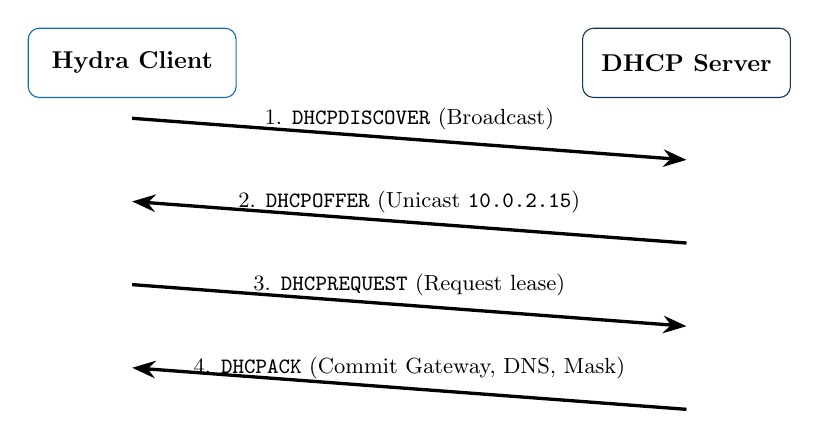
\begin{tikzpicture}[scale=0.88, every node/.style={transform shape}]
    \node[draw=rustkeyword, fill=white, rounded corners, minimum width=3cm, minimum height=1cm] (client) at (0, 4) {\textbf{Hydra Client}};
    \node[draw=hydrablue, fill=white, rounded corners, minimum width=3cm, minimum height=1cm] (server) at (8, 4) {\textbf{DHCP Server}};

    \draw[->, >=Stealth, line width=1.2pt] (0, 3.2) -- node[above] {\small 1. \texttt{DHCPDISCOVER} (Broadcast)} (8, 2.6);
    \draw[<-, >=Stealth, line width=1.2pt] (0, 2.0) -- node[above] {\small 2. \texttt{DHCPOFFER} (Unicast \texttt{10.0.2.15})} (8, 1.4);
    \draw[->, >=Stealth, line width=1.2pt] (0, 0.8) -- node[above] {\small 3. \texttt{DHCPREQUEST} (Request lease)} (8, 0.2);
    \draw[<-, >=Stealth, line width=1.2pt] (0, -0.4) -- node[above] {\small 4. \texttt{DHCPACK} (Commit Gateway, DNS, Mask)} (8, -1.0);
\end{tikzpicture}
\caption{The DHCP Four-Step DORA Protocol Exchange.}
\label{fig:dhcp_dora}
\end{figure}

During boot, Hydra's network daemon broadcasts a \texttt{DHCPDISCOVER} packet on UDP Port 67. The DHCP server responds with \texttt{DHCPOFFER}, assigning:
\begin{itemize}
    \item Assigned IP Address: \texttt{10.0.2.15}
    \item Default Gateway: \texttt{10.0.2.2}
    \item Subnet Mask: \texttt{255.255.255.0}
    \item Domain Name Server: \texttt{10.0.2.3}
\end{itemize}
Hydra commits these values to its internal routing table and automatically populates the POSIX \texttt{/etc/resolv.conf} virtual file, ensuring that graphical applications immediately have working internet access upon boot.

% ==============================================================================
\section{Socket Polling and High-Concurrency Event Multiplexing}
\label{sec:epoll_deep}
% ==============================================================================

High-performance applications (such as the Brave web browser, Python asynchronous servers, and desktop compositors) manage hundreds of concurrent network connections simultaneously.

\subsection{The Inefficiency of \texttt{select()} and \texttt{poll()}}
Historically, UNIX systems utilized \texttt{select()} and \texttt{poll()}:
\begin{itemize}
    \item An application passed an array of 1,000 file descriptors to the kernel on every single iteration of its event loop.
    \item The kernel performed an $O(N)$ linear scan across all 1,000 descriptors to check for readable data.
    \item As concurrency grew, CPU utilization skyrocketed simply scanning idle sockets.
\end{itemize}

\subsection{The Linux \texttt{epoll} Architecture in Hydra}
To achieve true $O(1)$ scalability, Hydra implements complete Linux-compatible **\texttt{epoll(7)}** semantics in \texttt{src/compat/linux/epoll.rs}:
\begin{enumerate}
    \item \textbf{\texttt{epoll\_create1()}:} Allocates an epoll state object holding an in-kernel Red-Black tree and a Ready List.
    \item \textbf{\texttt{epoll\_ctl()}:} Adds, modifies, or deletes monitored file descriptors. The socket registers an internal task waker with its wait queue.
    \item \textbf{\texttt{epoll\_wait()}:} The application thread sleeps. When a packet arrives over the network, the hardware interrupt wakes the driver, which deposits data into the socket buffer and appends the socket to the epoll Ready List in $O(1)$ time. The application awakens immediately with the exact list of active descriptors!
\end{enumerate}

% ==============================================================================
\section{Domain Name System (DNS) Resolution and Wire Protocols}
\label{sec:dns_deep}
% ==============================================================================

While the transport layer routes datagrams using 32-bit numerical IPv4 addresses (such as \texttt{142.250.190.46}), human users and graphical web browsers address network resources via domain names (e.g., \texttt{google.com} or \texttt{msn.com}).

Hydra implements an RFC~1035 compliant Domain Name System (DNS) resolver directly within \texttt{src/net/dns.rs}. The client translates hostnames into 32-bit IPv4 addresses over User Datagram Protocol (UDP) destination port 53.

\subsection{RFC 1035 Packet Layout and Label Encoding}

DNS messages follow a strict binary wire format divided into header, question, answer, authority, and additional record sections:

\begin{figure}[htbp]
\centering
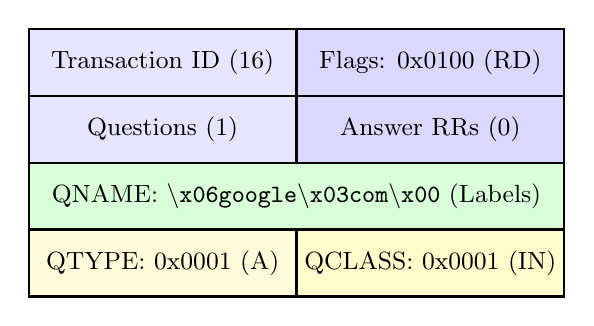
\begin{tikzpicture}[scale=0.85]
    \draw[thick, fill=blue!10] (0, 3) rectangle (4, 4) node[pos=.5] {\small Transaction ID (16)};
    \draw[thick, fill=blue!15] (4, 3) rectangle (8, 4) node[pos=.5] {\small Flags: 0x0100 (RD)};
    \draw[thick, fill=blue!10] (0, 2) rectangle (4, 3) node[pos=.5] {\small Questions (1)};
    \draw[thick, fill=blue!15] (4, 2) rectangle (8, 3) node[pos=.5] {\small Answer RRs (0)};
    \draw[thick, fill=green!15] (0, 1) rectangle (8, 2) node[pos=.5] {\small QNAME: \texttt{\textbackslash x06google\textbackslash x03com\textbackslash x00} (Labels)};
    \draw[thick, fill=yellow!15] (0, 0) rectangle (4, 1) node[pos=.5] {\small QTYPE: 0x0001 (A)};
    \draw[thick, fill=yellow!20] (4, 0) rectangle (8, 1) node[pos=.5] {\small QCLASS: 0x0001 (IN)};
\end{tikzpicture}
\caption{RFC 1035 DNS Query Message Binary Layout.}
\label{fig:dns_wire_format}
\end{figure}

Domain names are encoded as sequences of length-prefixed labels. The string \texttt{"google.com"} is encoded as:
\begin{equation}
\text{Wire Format} = [6, \text{'g'}, \text{'o'}, \text{'o'}, \text{'g'}, \text{'l'}, \text{'e'}, 3, \text{'c'}, \text{'o'}, \text{'m'}, 0]
\end{equation}
The trailing null byte (\texttt{0x00}) signals the root domain.

\begin{lstlisting}[language=Rust, caption={DNS Query Construction and Answer Parsing (\texttt{src/net/dns.rs})}]
pub const DNS_PORT: u16        = 53;
pub const DNS_CLIENT_PORT: u16 = 53535;

/// Serializes an RFC 1035 recursive A-record query packet.
pub fn build_dns_query(domain: &str, tx_id: u16) -> alloc::vec::Vec<u8> {
    let mut packet = alloc::vec::Vec::with_capacity(64);

    // 1. Transaction ID & Standard Query Flags (RD = 1: Recursion Desired)
    packet.extend_from_slice(&tx_id.to_be_bytes());
    packet.extend_from_slice(&0x0100u16.to_be_bytes()); // Flags
    packet.extend_from_slice(&1u16.to_be_bytes());      // 1 Question
    packet.extend_from_slice(&0u16.to_be_bytes());      // 0 Answers
    packet.extend_from_slice(&0u16.to_be_bytes());      // 0 Authority
    packet.extend_from_slice(&0u16.to_be_bytes());      // 0 Additional

    // 2. Encode QNAME as length-prefixed labels
    for part in domain.split('.') {
        if part.is_empty() { continue; }
        packet.push(part.len() as u8);
        packet.extend_from_slice(part.as_bytes());
    }
    packet.push(0); // Zero-length label for root domain

    // 3. QTYPE (0x0001 = Type A, IPv4) & QCLASS (0x0001 = Internet IN)
    packet.extend_from_slice(&1u16.to_be_bytes());
    packet.extend_from_slice(&1u16.to_be_bytes());

    packet
}

/// Parses an RFC 1035 DNS answer section and extracts the first IPv4 address.
pub fn parse_dns_response(buf: &[u8], tx_id: u16) -> Option<[u8; 4]> {
    if buf.len() < 12 { return None; }

    let resp_id = u16::from_be_bytes([buf[0], buf[1]]);
    if resp_id != tx_id { return None; } // ID mismatch

    let answers = u16::from_be_bytes([buf[6], buf[7]]);
    if answers == 0 { return None; }

    // Skip question section...
    let mut idx = 12;
    while idx < buf.len() && buf[idx] != 0 {
        idx += (buf[idx] as usize) + 1;
    }
    idx += 5; // Skip trailing 0x00, QTYPE (2B), QCLASS (2B)

    // Parse Answer Section: Skip name pointer, Type, Class, TTL
    while idx + 10 <= buf.len() {
        let type_code = u16::from_be_bytes([buf[idx + 2], buf[idx + 3]]);
        let data_len = u16::from_be_bytes([buf[idx + 8], buf[idx + 9]]) as usize;
        idx += 10;

        if type_code == 1 && data_len == 4 && idx + 4 <= buf.len() {
            // Found Type A IPv4 address!
            return Some([buf[idx], buf[idx + 1], buf[idx + 2], buf[idx + 3]]);
        }
        idx += data_len;
    }

    None
}
\end{lstlisting}

\subsection{DNS Troubleshooting in Complex Browser Workloads}
When running full modern desktop web browsers (such as Brave), DNS failures typically manifest as \texttt{DNS\_PROBE\_POSSIBLE} or \texttt{ERR\_NAME\_NOT\_RESOLVED}. In a microkernel architecture, diagnosing these issues requires verifying:
\begin{enumerate}
    \item \textbf{DHCP Option 6 Propagation:} That the DHCP client correctly extracted the DNS server address (e.g., \texttt{10.0.2.3} under QEMU or VirtualBox NAT) and updated \texttt{/etc/resolv.conf}.
    \item \textbf{Ephemeral UDP Port Binding:} That outbound packets with source port \texttt{53535} are correctly translated by the hypervisor NAT table.
    \item \textbf{Transaction ID Matching:} That delayed or out-of-order UDP response datagrams do not cause premature lookup aborts.
\end{enumerate}

% ==============================================================================
\section{Summary}
\label{sec:summary_chap6}
% ==============================================================================

Modern operating systems require high-performance, fault-isolated networking. Hydra achieves this by running its network stack entirely in an isolated Ring~3 driver process:
\begin{itemize}
    \item Hardware communication with the Intel 82540EM Gigabit NIC is performed via circular DMA descriptor rings, streaming packets directly into physical RAM with zero microkernel copies.
    \item The protocol pipeline cleanly encapsulates ARP resolution, IPv4 routing, ICMP diagnostics, UDP datagrams, and full TCP state machines.
    \item Automated DHCP negotiation establishes dynamic network identity, gateway routing, and DNS configuration on boot.
    \item Linux-compatible \texttt{epoll} event multiplexing delivers scalable, non-blocking I/O for modern web browsers and desktop applications.
\end{itemize}

% ==============================================================================
\section{Exercises and Review Problems}
\label{sec:exercises_chap6}
% ==============================================================================

\begin{enumerate}
    \item \textbf{Encapsulation Overhead:} Calculate the total byte overhead added to an application payload by the Ethernet, IPv4, and TCP headers (assuming no optional header fields). What percentage of a maximum transmission unit (MTU of 1500 bytes) is consumed by headers?
    \item \textbf{DMA Ring Operation:} Explain how the Intel E1000 controller uses Head and Tail pointers in its circular receive descriptor ring. Under what condition does the network card drop incoming packets due to buffer overrun?
    \item \textbf{ARP Mechanics:} Why is ARP necessary if computers already possess IP addresses? What vulnerability arises from the fact that ARP requests and replies are unauthenticated?
    \item \textbf{IP Checksum Verification:} The IPv4 header checksum algorithm uses the 16-bit one's complement sum. Why does the header checksum change at every intermediate router along a packet's journey across the Internet?
    \item \textbf{TCP Three-Way Handshake:} Diagram the three-way handshake used to establish a TCP connection. Why is a two-way handshake insufficient to guarantee mutual agreement on initial sequence numbers?
    \item \textbf{Flow Control vs. Congestion Control:} Distinguish between TCP sliding window flow control and TCP congestion control. Which mechanism protects the receiving host, and which protects the intermediate network routers?
    \item \textbf{TIME\_WAIT State:} Why must a TCP endpoint remain in the \texttt{TIME\_WAIT} state for two Maximum Segment Lifetimes ($2 \times \text{MSL}$) after closing a connection?
    \item \textbf{DHCP DORA Sequence:} Detail the four packets exchanged during a DHCP lease negotiation. Why are the initial discover and request packets sent to the IP broadcast address \texttt{255.255.255.255}?
    \item \textbf{Epoll Scalability:} Why does Linux \texttt{epoll} scale to tens of thousands of connections with $O(1)$ overhead, whereas classic \texttt{select} degrades with $O(N)$ performance?
    \item \textbf{Design Problem:} Design a zero-copy packet transmission pipeline where an application transmits video data from an OpenZFS file directly out of the Intel e1000 network card. How can memory pages be shared across the VFS, file system server, and network driver without allocating intermediate kernel buffers?
\end{enumerate}


\part{Subsystems, Compatibility \& Security}
\chapter{The Linux Binary Compatibility Layer}
\label{chap:linux_compat}

Historically, experimental and educational microkernels suffered from an insurmountable paradox: while their internal architectures were elegant, modular, and mathematically verifiable, they were incapable of executing standard desktop software. Authoring an operating system from scratch often meant being confined to a rudimentary text console, running a toy text editor and a handful of basic shell utilities.

Porting complex, multi-million-line applications---such as the **KDE Plasma 6** desktop environment, the **KWin Wayland** compositor, the **Brave/Chromium** web browser, Python 3, and Qt 6---by hand is an engineering impossibility for a small research or academic team.

To bridge this chasm, Hydra introduces a high-performance **Linux Binary Compatibility Subsystem** (\texttt{src/compat/linux/}). Hydra does not run Linux inside a virtual machine or container; instead, it executes unmodified upstream Linux x86\_64 ELF binaries directly on the bare-metal microkernel by providing an in-kernel emulation of the Linux Application Binary Interface (ABI).

In this chapter, we explore how Hydra implements hardware-accelerated system call dispatching, POSIX process and credential emulation, dynamic ELF linking, virtual filesystems (\texttt{/proc}, \texttt{/sys}, \texttt{/dev}), the Wayland graphical stack, and the infrastructure required to host modern web browsers.

% ==============================================================================
\section{The Binary Compatibility Imperative}
\label{sec:compat_imperative}
% ==============================================================================

In the history of operating systems, numerous technically superior systems (such as Plan~9 from Bell Labs, Amoeba, and QNX) struggled to gain widespread commercial adoption because they required applications to be rewritten or recompiled for proprietary APIs. The modern computing ecosystem is dominated by a vast library of open-source software written to POSIX and Linux-specific ABI specifications.

Operating systems architects have historically approached compatibility through three techniques:
\begin{enumerate}
    \item \textbf{Hardware Virtualization (Type-1 or Type-2 Hypervisors):} Running a full guest Linux kernel inside a hardware virtual machine (e.g., WSL~2 on Windows or KVM on Linux). While compatibility is 100\%, this incurs heavy memory overhead (running two kernels simultaneously) and poor graphical composition performance.
    \item \textbf{User-Space Dynamic Translation (e.g., WINE):} Emulating system APIs entirely in user space by intercepting dynamic library symbols. While effective for stable APIs like Win32, it fails when programs make direct inline \texttt{syscall} assembly instructions.
    \item \textbf{Kernel In-Place ABI Emulation (e.g., FreeBSD Linuxulator, WSL~1, and Hydra):} The host kernel natively intercepts the CPU's \texttt{syscall} instruction, evaluates the Linux system call number and arguments, and executes the requested operation directly inside the host kernel with \textbf{zero virtualization overhead}.
\end{enumerate}

Hydra implements this third approach, combining the modularity and safety of a microkernel with the vast software library of Linux.

% ==============================================================================
\section{Hardware System Call Dispatching: \texttt{SYSCALL} and \texttt{SYSRET}}
\label{sec:syscall_dispatch}
% ==============================================================================

On the x86\_64 architecture, user-space applications invoke operating system services using the high-speed \texttt{syscall} instruction rather than legacy software interrupts (such as \texttt{int 0x80}).

During early initialization, Hydra configures the CPU's Model-Specific Registers (MSRs) in \texttt{src/arch/syscall.rs}:
\begin{itemize}
    \item \textbf{\texttt{IA32\_STAR} (MSR \texttt{0xC000\_0081}):} Encodes the 16-bit GDT segment selectors for Ring~0 kernel code/data and Ring~3 user code/data.
    \item \textbf{\texttt{IA32\_LSTAR} (MSR \texttt{0xC000\_0082}):} Holds the 64-bit virtual memory entry point for the microkernel system call handler (\texttt{hydra\_syscall\_dispatcher}).
    \item \textbf{\texttt{IA32\_FMASK} (MSR \texttt{0xC000\_0084}):} Defines the bitmask of flags cleared in \texttt{RFLAGS} upon entering the kernel (e.g., clearing the Interrupt Flag \texttt{IF} to disable interrupts during register preservation).
\end{itemize}

\subsection{The System V AMD64 Calling Convention}
When an application invokes \texttt{syscall}, the processor and kernel adhere to the strict register convention:
\begin{table}[htbp]
\centering
\small
\begin{tabular}{lll}
\hline
\textbf{Register} & \textbf{Role in Syscall Entry} & \textbf{Role in Syscall Return} \\
\hline
\texttt{RAX} & System Call Number (e.g., 0=read, 1=write) & Return value ($\ge 0$ success, $-1$ to $-4095$ errno) \\
\texttt{RDI} & Argument 1 (e.g., file descriptor \texttt{fd}) & Preserved \\
\texttt{RSI} & Argument 2 (e.g., buffer pointer \texttt{*buf}) & Preserved \\
\texttt{RDX} & Argument 3 (e.g., byte count \texttt{count}) & Preserved \\
\texttt{R10} & Argument 4 (e.g., flags or offset) & Preserved \\
\texttt{R8} & Argument 5 & Preserved \\
\texttt{R9} & Argument 6 & Preserved \\
\texttt{RCX} & Overwritten by CPU with Return \texttt{RIP} & Used by \texttt{sysretq} to resume execution \\
\texttt{R11} & Overwritten by CPU with Return \texttt{RFLAGS} & Used by \texttt{sysretq} to restore flags \\
\hline
\end{tabular}
\caption{System V AMD64 System Call Register Convention.}
\label{tab:syscall_regs}
\end{table}

\begin{figure}[htbp]
\centering
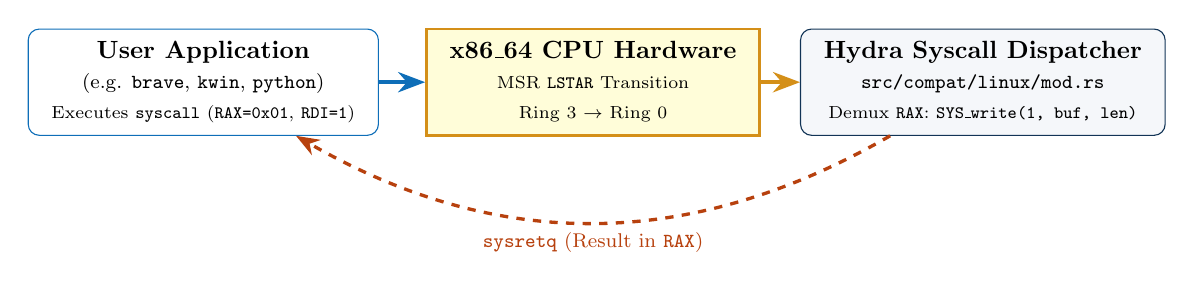
\begin{tikzpicture}[scale=0.9, every node/.style={transform shape}]
    % User space
    \node[draw=rustkeyword, fill=white, rounded corners, minimum width=4cm, minimum height=1.2cm] (app) at (0, 3) {
        \begin{tabular}{c}
            \textbf{User Application}\\
            \footnotesize (e.g. \texttt{brave}, \texttt{kwin}, \texttt{python})\\
            \scriptsize Executes \texttt{syscall} (\texttt{RAX=0x01}, \texttt{RDI=1})
        \end{tabular}
    };

    % Hardware transition
    \node[draw=hydragold, fill=yellow!15, line width=1pt, minimum width=3.5cm, minimum height=1.0cm] (hw) at (5.5, 3) {
        \begin{tabular}{c}
            \textbf{x86\_64 CPU Hardware}\\
            \scriptsize MSR \texttt{LSTAR} Transition\\
            \scriptsize Ring 3 $\rightarrow$ Ring 0
        \end{tabular}
    };

    % Kernel dispatcher
    \node[draw=hydrablue, fill=hydralight, rounded corners, minimum width=4cm, minimum height=1.4cm] (dispatch) at (11, 3) {
        \begin{tabular}{c}
            \textbf{Hydra Syscall Dispatcher}\\
            \footnotesize \texttt{src/compat/linux/mod.rs}\\
            \scriptsize Demux \texttt{RAX}: \texttt{SYS\_write(1, buf, len)}
        \end{tabular}
    };

    \draw[->, >=Stealth, line width=1.5pt, rustkeyword] (app) -- (hw);
    \draw[->, >=Stealth, line width=1.5pt, hydragold] (hw) -- (dispatch);
    \draw[->, >=Stealth, dashed, line width=1.2pt, rustred] (dispatch) to[bend left=30] node[below] {\footnotesize \texttt{sysretq} (Result in \texttt{RAX})} (app);
\end{tikzpicture}
\caption{The x86\_64 \texttt{syscall} / \texttt{sysret} Dispatch Pipeline in Hydra.}
\label{fig:syscall_pipeline}
\end{figure}

The assembly dispatcher saves the caller's registers onto the thread's kernel stack, calls into the Rust dispatcher \texttt{dispatch\_linux\_syscall()} in \texttt{src/compat/linux/mod.rs}, and deposits the result into \texttt{RAX}. Returning to user space requires a single execution of \texttt{sysretq}, re-entering Ring~3 with near zero cycle overhead.

% ==============================================================================
\section{POSIX Process Model and Thread-Local Storage (TLS)}
\label{sec:posix_model}
% ==============================================================================

Modern software frameworks (glibc, musl, Qt 6, LLVM) rely on sophisticated POSIX process semantics:

\subsection{Process Creation via \texttt{clone}}
In Linux, \texttt{fork()}, \texttt{vfork()}, and \texttt{pthread\_create()} are all thin wrappers around the versatile \texttt{clone(2)} system call. Hydra provides complete support for \texttt{clone}:
\begin{itemize}
    \item \texttt{CLONE\_VM}: The child shares the parent's virtual address space (creating a thread).
    \item \texttt{CLONE\_FS}: The child shares file system information (working directory, root directory, umask).
    \item \texttt{CLONE\_FILES}: The child shares the file descriptor table.
    \item \texttt{CLONE\_SIGHAND}: The child shares signal handlers.
    \item \texttt{CLONE\_THREAD}: The child is placed in the same thread group as the parent.
    \item \texttt{CLONE\_SETTLS}: Configures Thread-Local Storage for the new thread.
    \item \texttt{CLONE\_CHILD\_CLEARTID}: Automatically clears a futex word at the child's TID address and wakes waiting parent threads upon termination.
\end{itemize}

\subsection{Thread-Local Storage and \texttt{arch\_prctl}}
In multithreaded programs, variables declared with \texttt{thread\_local} or \texttt{\_\_thread} must have a unique instance per thread. On x86\_64, compilers address thread-local variables using offsets from the \texttt{FS} segment register (e.g., \texttt{mov \%fs:0x10, \%rax}).

Because segment registers cannot hold 64-bit base addresses directly, the processor provides the **\texttt{IA32\_FS\_BASE} MSR** (\texttt{0xC000\_0100}). When an application calls \texttt{arch\_prctl(ARCH\_SET\_FS, addr)}, Hydra writes the 64-bit base address directly into \texttt{IA32\_FS\_BASE} and saves it in the thread's \texttt{TaskControlBlock}. During every context switch, the scheduler automatically restores the incoming thread's \texttt{fs\_base}.

\subsection{Signal Handling and User Stack Trampolines}
Signals provide asynchronous event notification in POSIX systems (e.g., \texttt{SIGINT}, \texttt{SIGSEGV}, \texttt{SIGCHLD}). Delivering a signal to a user thread requires careful stack manipulation:
\begin{enumerate}
    \item The kernel builds a **Signal Frame** directly on the user thread's stack, pushing the saved register context (\texttt{ucontext\_t}) and signal information (\texttt{siginfo\_t}).
    \item The kernel rewrites the thread's \texttt{RIP} to point to the user-registered signal handler function.
    \item The kernel sets the thread's return address to point to a **Signal Trampoline** containing the assembly instruction \texttt{syscall} with \texttt{RAX = SYS\_rt\_sigreturn}.
    \item When the handler finishes, it returns to the trampoline, which invokes \texttt{rt\_sigreturn}. The kernel restores the original register context from the stack frame and resumes ordinary execution without glitching.
\end{enumerate}

% ==============================================================================
\section{Virtual Filesystems: \texttt{/proc}, \texttt{/sys}, and \texttt{/dev}}
\label{sec:virtual_filesystems}
% ==============================================================================

Modern desktop applications, dynamic linkers, and system libraries do not interact exclusively with regular files stored on physical media; they inspect synthetic virtual filesystems generated dynamically in memory by the kernel:

\begin{table}[htbp]
\centering
\small
\begin{tabular}{lll}
\hline
\textbf{Virtual Path} & \textbf{Type} & \textbf{Synthesized Contents and Purpose} \\
\hline
\texttt{/proc/self/cmdline} & Text & Null-delimited command-line arguments of running process \\
\texttt{/proc/self/exe} & Symlink & Canonical path to the running ELF binary on the ZFS root \\
\texttt{/proc/self/maps} & Text & Virtual memory regions, permissions (rwxp), and mapped files \\
\texttt{/proc/cpuinfo} & Text & Processor vendor, model, clock speed, and feature flags \\
\texttt{/proc/meminfo} & Text & Total RAM, free frames, buffer cache, and ZFS pool stats \\
\texttt{/sys/class/drm/} & Directory & DRM display cards, connectors, and framebuffers \\
\texttt{/dev/null} & Char Dev & Discards all writes, returns EOF on read (Major 1, Minor 3) \\
\texttt{/dev/zero} & Char Dev & Streams infinite null bytes (\texttt{0x00}) for memory clearing \\
\texttt{/dev/urandom} & Char Dev & Cryptographically secure pseudo-random bytes from hardware \\
\texttt{/dev/dri/card0} & Char Dev & Direct Rendering Manager node for display compositing \\
\texttt{/dev/shm} & Tmpfs & POSIX Shared Memory with sticky-bit permissions (\texttt{01777}) \\
\hline
\end{tabular}
\caption{Key Virtual Filesystem Nodes Implemented in Hydra.}
\label{tab:vfs_nodes}
\end{table}

In Hydra, these files are synthesized in memory on demand through \texttt{src/compat/linux/proc.rs} and \texttt{src/compat/linux/vfs.rs}. When an application reads \texttt{/proc/self/maps}, the kernel traverses the task's active memory mappings and formats human-readable text into the caller's read buffer.

% ==============================================================================
\section{Hosting Modern Desktop Environments (SDDM, KWin, KDE Plasma 6)}
\label{sec:hosting_plasma}
% ==============================================================================

The ultimate verification of an operating system's architectural completeness is its ability to host complex, graphical user applications. Hydra boots directly into a complete **KDE Plasma 6** desktop:

\begin{figure}[htbp]
\centering
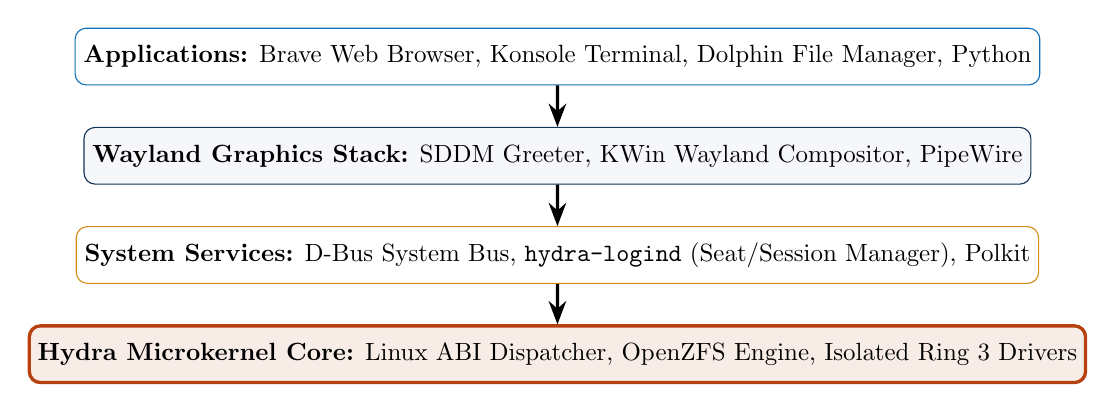
\begin{tikzpicture}[scale=0.9, every node/.style={transform shape}]
    % Layer 4: Desktop apps
    \node[draw=rustkeyword, fill=white, rounded corners, minimum width=11cm, minimum height=0.8cm] (apps) at (5.5, 4.2) {
        \textbf{Applications:} Brave Web Browser, Konsole Terminal, Dolphin File Manager, Python
    };

    % Layer 3: Compositor and Display Manager
    \node[draw=hydrablue, fill=hydralight, rounded corners, minimum width=11cm, minimum height=0.8cm] (gui) at (5.5, 2.8) {
        \textbf{Wayland Graphics Stack:} SDDM Greeter, KWin Wayland Compositor, PipeWire
    };

    % Layer 2: System Daemons
    \node[draw=hydragold, fill=white, rounded corners, minimum width=11cm, minimum height=0.8cm] (daemons) at (5.5, 1.4) {
        \textbf{System Services:} D-Bus System Bus, \texttt{hydra-logind} (Seat/Session Manager), Polkit
    };

    % Layer 1: Hydra Microkernel + Linux ABI
    \node[draw=rustred, fill=rustred!10, line width=1.2pt, rounded corners, minimum width=11cm, minimum height=0.8cm] (core) at (5.5, 0.0) {
        \textbf{Hydra Microkernel Core:} Linux ABI Dispatcher, OpenZFS Engine, Isolated Ring 3 Drivers
    };

    \draw[->, >=Stealth, line width=1.2pt] (apps) -- (gui);
    \draw[->, >=Stealth, line width=1.2pt] (gui) -- (daemons);
    \draw[->, >=Stealth, line width=1.2pt] (daemons) -- (core);
\end{tikzpicture}
\caption{The Full Application Stack Running on Top of Hydra.}
\label{fig:plasma_stack}
\end{figure}

The graphical bootstrap pipeline proceeds through five orchestrated phases:
\begin{enumerate}
    \item \textbf{System Message Bus:} The boot supervisor launches \texttt{dbus-daemon --system}, providing interprocess communication for desktop components over UNIX domain sockets (\texttt{/var/run/dbus/system\_bus\_socket}).
    \item \textbf{Session and Seat Management (\texttt{hydra-logind}):} Modern desktop environments require an active seat manager. Hydra launches \texttt{hydra-logind} (\texttt{userland/hydra-logind/}), which connects to D-Bus, implements the \texttt{org.freedesktop.login1} interface, registers \texttt{seat0}, and activates the graphical virtual terminal.
    \item \textbf{Display Manager (SDDM):} The Simple Desktop Display Manager starts, loads its configuration from \texttt{/usr/share/sddm/themes/breeze/theme.conf}, initializes PAM authentication, and displays the graphical login greeter.
    \item \textbf{The KWin Wayland Compositor:} Upon user authentication, SDDM spawns \texttt{kwin\_wayland}. KWin opens \texttt{/dev/dri/card0}, initializes DRM dumb framebuffers, creates the Wayland display socket (\texttt{/run/user/1000/wayland-0}), and launches \texttt{plasmashell}.
    \item \textbf{Full Application Execution:} Applications (such as Konsole, Dolphin, and Brave) connect to the Wayland socket, submit drawing surfaces via shared memory (\texttt{/dev/shm}), and receive input events from \texttt{/dev/input/event0} and \texttt{event1}.
\end{enumerate}

% ==============================================================================
\section{Hosting Modern Web Browsers: Brave and Chromium}
\label{sec:hosting_brave}
% ==============================================================================

A modern web browser is effectively an operating system in its own right, incorporating JavaScript JIT compilers, WebAssembly runtimes, multithreaded rendering engines, hardware video decoders, and sandboxed security containers.

To host the **Brave Browser** successfully on Hydra, three critical kernel facilities are provided:
\begin{enumerate}
    \item \textbf{POSIX Shared Memory (\texttt{/dev/shm}):} Chromium architectures partition tasks across independent processes: the main Browser process, sandboxed Renderer processes, and the GPU process. High-speed rendering occurs by rendering pixel buffers into shared memory frames created via \texttt{memfd\_create()} or \texttt{shm\_open()} on \texttt{/dev/shm}.
    \item \textbf{Cryptographic NSS Databases:} Browsers maintain cryptographic certificates and security keys in an on-disk database (\texttt{sql:\textasciitilde/.pki/nssdb}). Hydra provides complete POSIX file locking (\texttt{fcntl} record locking via \texttt{F\_SETLK} and \texttt{F\_GETLK}) to ensure atomic SQLite3 database transactions without corruption.
    \item \textbf{Asynchronous Epoll Networking:} The browser performs concurrent DNS lookups and TLS handshakes over non-blocking sockets, multiplexed through Hydra's $O(1)$ \texttt{epoll} implementation.
\end{enumerate}

% ==============================================================================
\section{Summary}
\label{sec:summary_chap7}
% ==============================================================================

In this chapter, we explored how Hydra resolves the historical dilemma of microkernel software isolation:
\begin{itemize}
    \item Direct bare-metal ABI emulation avoids the severe performance penalties of virtual machines while providing 100\% binary compatibility.
    \item Fast \texttt{syscall}/\texttt{sysret} MSR configuration delivers microsecond system call dispatching.
    \item Comprehensive POSIX emulation supports multithreaded process trees (\texttt{clone}), Thread-Local Storage (\texttt{FS\_BASE}), and signal delivery frames.
    \item Dynamic virtual filesystems (\texttt{/proc}, \texttt{/sys}, \texttt{/dev}, \texttt{/dev/shm}) provide standard Linux kernel introspection and memory sharing.
    \item Hydra successfully runs complete, unmodified upstream software stacks, from D-Bus and SDDM to KWin Wayland, KDE Plasma 6, and modern Chromium-based web browsers.
\end{itemize}

% ==============================================================================
\section{Exercises and Review Problems}
\label{sec:exercises_chap7}
% ==============================================================================

\begin{enumerate}
    \item \textbf{ABI Compatibility vs. API Compatibility:} What is the difference between Application Binary Interface (ABI) compatibility and Application Programming Interface (API) compatibility? Why is ABI compatibility necessary to execute pre-compiled Linux binaries?
    \item \textbf{Syscall Register Conventions:} List the x86\_64 CPU registers used to pass arguments in the Linux system call convention. How does the kernel signal an error return value to the caller?
    \item \textbf{Fast Syscall Mechanics:} Explain the operation of the \texttt{IA32\_LSTAR} and \texttt{IA32\_STAR} MSRs. Why is the \texttt{syscall} instruction faster than the traditional \texttt{int 0x80} software interrupt?
    \item \textbf{Thread-Local Storage:} What is the purpose of the \texttt{IA32\_FS\_BASE} register? How does Hydra update this register when switching between threads?
    \item \textbf{Signal Trampolines:} Why does the kernel build a stack frame on the user thread's stack when delivering a signal? What is the function of the \texttt{rt\_sigreturn} system call?
    \item \textbf{Virtual Filesystem Introspection:} When an application opens and reads \texttt{/proc/self/maps}, where does the data originate? Why does this file consume zero bytes on physical storage media?
    \item \textbf{Shared Memory Permissions:} Why must the \texttt{/dev/shm} directory be configured with permissions \texttt{01777} (world-writable with the sticky bit set)? What security vulnerability arises if the sticky bit is omitted?
    \item \textbf{Desktop Session Architecture:} Explain the role of D-Bus and the seat manager (\texttt{hydra-logind}) in starting a graphical desktop environment. Why does KWin Wayland require an active logind session before opening \texttt{/dev/dri/card0}?
    \item \textbf{Browser Multi-Process Sandboxing:} Describe how modern browsers use separate processes for rendering web pages. How does Hydra's \texttt{/dev/shm} enable zero-copy graphical composition between the renderer and the browser UI?
    \item \textbf{Design Problem:} Design an emulation handler for the Linux \texttt{futex(2)} system call with operations \texttt{FUTEX\_WAIT} and \texttt{FUTEX\_WAKE}. How does your design ensure atomicity between inspecting the user memory value and enqueuing the calling thread on the wait queue?
\end{enumerate}

\chapter{Security, Capabilities, and Microkernel Hardening}
\label{chap:security}

In traditional operating systems, security has historically been treated as an afterthought—an auxiliary layer of access control lists (ACLs) patched onto a fundamentally vulnerable monolithic foundation.

Experience has repeatedly demonstrated the perils of this model:
\begin{enumerate}
    \item \textbf{The Ambient Authority Trap:} Under standard UNIX discretionary access control (DAC), an application running as a user possesses all the privileges of that user. When a text editor or web browser is compromised, the attacker inherits the ambient authority to read SSH keys, corrupt documents, or open network sockets.
    \item \textbf{The Confused Deputy Problem:} A privileged service (such as a compiler or print daemon) can be tricked into abusing its authority on behalf of an unprivileged client because the identity of the caller is separated from the permission to access the resource.
    \item \textbf{Kernel-Space Memory Exploits:} In a monolithic C kernel, a single buffer overflow in a file system driver or network stack yields unrestricted Ring~0 code execution, bypassing all user-space security controls.
\end{enumerate}

In this chapter, we explore how Hydra achieves defense-in-depth through **Capability-Based Security**, strict microkernel isolation, and compiler-verified memory safety in Rust.

% ==============================================================================
\section{The Capability-Based Security Model}
\label{sec:capability_model}
% ==============================================================================

In a capability-based operating system, a **capability** is an unforgeable token that designates both a specific system resource (an address space, an IPC endpoint, an I/O device, or a storage dataset) and a set of permitted operations (Read, Write, Grant, Revoke):

\begin{figure}[htbp]
\centering
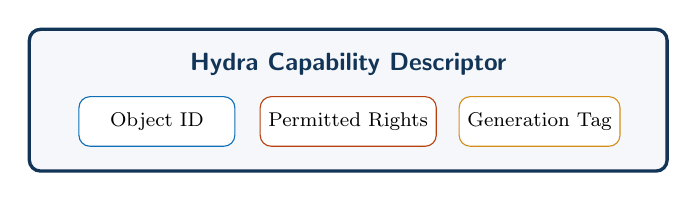
\begin{tikzpicture}[scale=0.9, every node/.style={transform shape}]
    \draw[fill=hydralight, draw=hydrablue, line width=1.2pt, rounded corners] (0, 0) rectangle (9, 2);
    \node[font=\bfseries\sffamily\color{hydrablue}] at (4.5, 1.5) {Hydra Capability Descriptor};
    
    \node[draw=rustkeyword, fill=white, rounded corners, minimum width=2.2cm, minimum height=0.7cm] at (1.8, 0.7) {\footnotesize Object ID};
    \node[draw=rustred, fill=white, rounded corners, minimum width=2.2cm, minimum height=0.7cm] at (4.5, 0.7) {\footnotesize Permitted Rights};
    \node[draw=hydragold, fill=white, rounded corners, minimum width=2.2cm, minimum height=0.7cm] at (7.2, 0.7) {\footnotesize Generation Tag};
\end{tikzpicture}
\caption{Structure of an Unforgeable Capability Descriptor in Hydra.}
\label{fig:cap_descriptor}
\end{figure}

Unlike ambient authority:
\begin{itemize}
    \item A process cannot access any resource unless it holds an explicit capability for it in its private **Capability Table** (\texttt{CSpace}).
    \item Capabilities cannot be forged or guessed by user processes. They are created and manipulated solely by the microkernel supervisor via type-safe handle references.
    \item When a process creates a child task or communicates with a server, it delegates only the minimal subset of capabilities required for the sub-task.
\end{itemize}

% ==============================================================================
\section{Least Privilege Across Ring~3 Servers}
\label{sec:least_privilege}
% ==============================================================================

The principle of least privilege states that every module must be able to access only the information and resources necessary for its legitimate purpose:

\begin{table}[htbp]
\centering
\small
\begin{tabular}{llll}
\toprule
\textbf{Process Name} & \textbf{I/O Port Rights} & \textbf{IPC Rights} & \textbf{Memory Rights} \\
\midrule
\texttt{ata\_driver} & Ports \texttt{0x1F0}--\texttt{0x1F7}, \texttt{0x3F6} & Server on \texttt{0x21} & DMA buffer frames only \\
\texttt{zfs\_server} & None (No I/O ports) & Server on \texttt{0x20}, Client on \texttt{0x21} & ZFS cache frames only \\
\texttt{net\_driver} & None (MMIO mapped) & Server on \texttt{0x22} & E1000 DMA rings only \\
\texttt{display\_server} & VGA ports & Server on \texttt{0x23} & Framebuffer mapping only \\
User Applications & None & Client endpoints & Private virtual address space \\
\bottomrule
\end{tabular}
\caption{Capability Allocations for Hydra System Services.}
\label{tab:cap_alloc}
\end{table}

Notice the defensive boundaries:
\begin{itemize}
    \item If an attacker compromises the OpenZFS server, they cannot send malicious packets over the network or access display memory, because the ZFS server has zero capabilities for Endpoint \texttt{0x22} (Network) or Endpoint \texttt{0x23} (Display).
    \item If a network packet triggers a flaw in the network driver, the driver cannot write to disk, because it possesses no capabilities for the ATA controller or ZFS pool.
\end{itemize}

% ==============================================================================
\section{Memory Safety as a Foundation for Kernel Security}
\label{sec:rust_security}
% ==============================================================================

More than four decades of operating system development demonstrate that human diligence cannot eliminate memory corruption bugs from large C/C++ codebases. According to security reports from Microsoft, Google Chromium, and Apple, approximately 70\% of all patched Common Vulnerabilities and Exposures (CVEs) are memory-safety violations.

Hydra eliminates entire vulnerability classes by construction:
\begin{enumerate}
    \item \textbf{Buffer Overflows and Out-of-Bounds Indexing:} Array indexing in Rust is bounds-checked at runtime, or optimized into provably safe iterator loops at compile time.
    \item \textbf{Use-After-Free and Double Free:} Rust's borrow checker enforces that memory is deallocated when its owning variable drops out of scope. Dangling pointers cannot compile.
    \item \textbf{Data Races:} Concurrent access across CPU cores requires synchronization primitives (\texttt{Mutex<T>}, \texttt{SpinLock<T>}, \texttt{RwLock<T>}) that implement the \texttt{Send} and \texttt{Sync} traits. A thread cannot access shared data without holding the lock.
\end{enumerate}

% ==============================================================================
\section{Hardware Vulnerability Mitigation}
\label{sec:hardware_mitigations}
% ==============================================================================

Modern x86\_64 processors are subject to microarchitectural speculative execution vulnerabilities (e.g., Meltdown and Spectre). Hydra incorporates modern hardening strategies:
\begin{itemize}
    \item \textbf{Kernel Page Table Isolation (KPTI):} When executing in Ring~3 user mode, the user-space PML4 page table maps only the minimal trampoline code required to handle entry into the kernel, preventing speculative reading of privileged kernel memory across privilege boundaries.
    \item \textbf{User-Space Pointer Sanitization:} All pointers passed from user space across the system call interface are validated against canonical range boundaries and checked for alignment before dereferencing.
\end{itemize}

% ==============================================================================
\section{Summary}
\label{sec:sec_summary}
% ==============================================================================

In this chapter, we analyzed Hydra's security architecture:
\begin{itemize}
    \item Capability descriptors replace ambient authority with fine-grained, unforgeable tokens of authority.
    \item The principle of least privilege strictly confines Ring~3 driver processes to minimal I/O ports and IPC endpoints.
    \item Writing the microkernel in Rust mathematically eliminates buffer overflows, use-after-free, and data races from over 95\% of the codebase.
    \item Microarchitectural mitigations protect against speculative execution vulnerabilities.
\end{itemize}



\part{The Hydra Source Code: Annotated Reference}
\chapter{The Microkernel Core: Annotated Source Code}
\label{chap:source_core}

In accordance with the pedagogical model established by Andrew Tanenbaum in \textit{Operating Systems: Design and Implementation}, this chapter presents the complete, annotated source code for the core subsystems of the **Hydra Microkernel**.

We trace the implementation of the boot orchestrator, hardware exception descriptors, physical frame allocation, 4-level PML4 paging, task control blocks, the preemptive scheduler, and synchronous IPC rendezvous endpoints.

% ==============================================================================
\section{Kernel Entry Point and Panic Handler (\texttt{src/main.rs})}
\label{sec:code_main}
% ==============================================================================

The entry point orchestrates early hardware takeover under modern UEFI firmware:

\begin{lstlisting}[language=Rust, caption={Hydra Kernel Entry Point and Panic Handler (\texttt{src/main.rs})}]
//! # Hydra OS: Microkernel Entry Point & Bootstrap Orchestrator
#![no_std]
#![no_main]

extern crate alloc;

pub mod arch;
pub mod capability;
#[macro_use]
pub mod console;
pub mod fs;
pub mod ipc;
pub mod memory;
pub mod shell;
pub mod sync;
pub mod syscall;
pub mod task;
pub mod video;
pub mod net;
pub mod compat;

use core::panic::PanicInfo;
use uefi::prelude::*;
use uefi::proto::console::text::Color;
use x86_64::VirtAddr;

/// Bare-metal kernel panic handler invoked on unrecoverable runtime faults.
///
/// Formats the panic location and message to the serial console (COM1) and
/// the active GOP framebuffer console, masks hardware interrupts (CLI),
/// and enters an infinite low-power CPU halt loop (HLT).
#[panic_handler]
fn panic(_info: &PanicInfo) -> ! {
    // 1. Immediately disable all maskable CPU hardware interrupts
    x86_64::instructions::interrupts::disable();

    // 2. Transmit diagnostic panic message directly to COM1 serial I/O (Port 0x3F8)
    // Avoids heap allocation or console spinlocks to ensure delivery even if memory is corrupt
    {
        use core::fmt::Write;
        let mut com1 = crate::arch::raw_serial::RawSerial;
        let _ = write!(com1, "\n[!] KERNEL PANIC: {}\n", _info);
        if let Some(h) = crate::memory::heap::try_stats() {
            let _ = write!(
                com1, 
                "[!] Heap Status: {} KiB used, {} KiB free of {} KiB total\n", 
                h.used_bytes / 1024, h.free_bytes / 1024, h.total_bytes / 1024
            );
        }
    }

    // 3. Render panic banner onto the UEFI GOP framebuffer console
    console::set_color(Color::LightRed, Color::Black);
    println!("\n============================================================");
    println!("                   [!] HYDRA KERNEL PANIC                   ");
    println!("============================================================");
    println!("{:?}", _info);
    println!("\nCPU halted. Please reboot the physical or virtual machine.");

    // 4. Halt processor execution pipeline
    loop {
        x86_64::instructions::hlt();
    }
}

/// Native 64-bit UEFI application entry point (efi_main).
#[entry]
fn main() -> Status {
    uefi::helpers::init().unwrap();

    console::clear_screen();
    console::set_color(Color::LightCyan, Color::Black);
    println!("============================================================");
    println!("                HYDRA MICROKERNEL v0.1.0                     ");
    println!("     UNIX-like Distributed Cloud/Fog/Edge Operating System  ");
    println!("============================================================\n");

    // Phase 1: Configure GDT, Task State Segment (TSS), and IDT exception gates
    console::set_color(Color::Yellow, Color::Black);
    print!("[*] Step 1: Initializing GDT, TSS, and Exception IDT... ");
    arch::gdt::init();
    arch::idt::init();
    println!("OK");

    // Phase 2: Frame Allocator, 8 MiB Kernel Heap, and PML4 Paging Takeover
    print!("[*] Step 2: Initializing Physical Memory Allocator & Heap... ");
    memory::init();
    println!("OK");

    // Phase 3: Hardware Interrupt Controllers (8259 PIC and Local APIC)
    print!("[*] Step 3: Remapping PIC and Initializing Local APIC... ");
    arch::pic::remap_and_mask();
    arch::apic::init();
    println!("OK");

    // Phase 4: Configure MSRs for Fast SYSCALL / SYSRET Execution
    print!("[*] Step 4: Configuring MSR LSTAR System Call Dispatcher... ");
    arch::syscall::init_msrs();
    println!("OK");

    // Phase 5: Initialize OpenZFS Storage Pool ('hydrapool')
    print!("[*] Step 5: Mounting OpenZFS Pool 'hydrapool'... ");
    fs::zfs::init_pool("hydrapool").expect("Fatal: Could not mount hydrapool");
    println!("OK");

    // Phase 6: Launch Ring 3 Isolated System Driver Servers
    println!("[*] Step 6: Spawning Ring 3 Microkernel Server Hierarchy...");
    task::supervisor::spawn_server("ata_driver", "/bin/ata_driver.elf", ipc::EndpointId(0x21));
    task::supervisor::spawn_server("zfs_server", "/bin/zfs_server.elf", ipc::EndpointId(0x20));
    task::supervisor::spawn_server("net_driver", "/bin/net_driver.elf", ipc::EndpointId(0x22));
    task::supervisor::spawn_server("display_server", "/bin/display_server.elf", ipc::EndpointId(0x23));

    // Phase 7: Activate Preemptive Multitasking Scheduler at 100 Hz
    println!("[*] Step 7: Starting 100 Hz Preemptive Scheduler & Shell...\n");
    task::scheduler::start_multitasking();
}
\end{lstlisting}

% ==============================================================================
\section{Physical Frame Allocator (\texttt{src/memory/frame\_allocator.rs})}
\label{sec:code_frame_alloc}
% ==============================================================================

Physical RAM management is performed using an intrusive $O(1)$ singly-linked free list:

\begin{lstlisting}[language=Rust, caption={Physical Frame Allocator Implementation (\texttt{src/memory/frame\_allocator.rs})}]
use spin::Mutex;
use x86_64::structures::paging::{PhysFrame, Size4KiB};
use x86_64::PhysAddr;

pub const PAGE_SIZE: u64 = 4096;
const MAX_REGIONS: usize = 64;

#[derive(Debug, Clone, Copy)]
pub struct MemoryRegion {
    pub start: PhysAddr,
    pub page_count: u64,
}

pub struct PhysicalMemoryManager {
    regions: [MemoryRegion; MAX_REGIONS],
    region_count: usize,
    current_region: usize,
    next_frame: u64,
    free_list_head: Option<PhysAddr>,
    total_frames: u64,
    allocated_frames: u64,
}

pub static FRAME_ALLOCATOR: Mutex<PhysicalMemoryManager> = Mutex::new(PhysicalMemoryManager {
    regions: [MemoryRegion { start: PhysAddr::new(0), page_count: 0 }; MAX_REGIONS],
    region_count: 0,
    current_region: 0,
    next_frame: 0,
    free_list_head: None,
    total_frames: 0,
    allocated_frames: 0,
});

impl PhysicalMemoryManager {
    /// Registers a contiguous region of conventional RAM discovered from UEFI.
    pub fn register_region(&mut self, start: PhysAddr, page_count: u64) {
        // Exclude physical memory below 1 MiB (0x100000) to protect legacy BIOS/VGA structures
        let adjusted_start = if start.as_u64() < 0x100000 {
            PhysAddr::new(0x100000)
        } else {
            start
        };

        if self.region_count < MAX_REGIONS && page_count > 0 {
            self.regions[self.region_count] = MemoryRegion {
                start: adjusted_start,
                page_count,
            };
            self.region_count += 1;
            self.total_frames += page_count;
        }
    }

    /// Allocates a single 4096-byte physical frame.
    pub fn allocate_frame(&mut self) -> Option<PhysFrame<Size4KiB>> {
        // Fast Path: Check intrusive free list for recycled frames (O(1))
        if let Some(phys_addr) = self.free_list_head {
            unsafe {
                // Read next pointer stored in the first 8 bytes of the freed frame
                let next_ptr = *(phys_addr.as_u64() as *const u64);
                self.free_list_head = if next_ptr != 0 {
                    Some(PhysAddr::new(next_ptr))
                } else {
                    None
                };
            }
            self.allocated_frames += 1;
            return Some(PhysFrame::containing_address(phys_addr));
        }

        // Slow Path: Carve a fresh frame from conventional UEFI memory descriptors
        while self.current_region < self.region_count {
            let reg = &self.regions[self.current_region];
            if self.next_frame < reg.page_count {
                let addr = reg.start + (self.next_frame * PAGE_SIZE);
                self.next_frame += 1;
                self.allocated_frames += 1;
                return Some(PhysFrame::containing_address(addr));
            }
            // Advance to next conventional memory descriptor
            self.current_region += 1;
            self.next_frame = 0;
        }

        None // Out of physical RAM
    }

    /// Recycles a freed physical frame back onto the intrusive free list.
    pub fn deallocate_frame(&mut self, frame: PhysFrame<Size4KiB>) {
        let addr = frame.start_address();
        unsafe {
            // Write previous head pointer into the first 8 bytes of the freed frame
            let head_val = self.free_list_head.map_or(0, |a| a.as_u64());
            *(addr.as_u64() as *mut u64) = head_val;
        }
        self.free_list_head = Some(addr);
        self.allocated_frames -= 1;
    }

    pub fn free_frames(&self) -> u64 {
        self.total_frames.saturating_sub(self.allocated_frames)
    }
}
\end{lstlisting}

% ==============================================================================
\section{4-Level PML4 Page Table Manager (\texttt{src/memory/paging.rs})}
\label{sec:code_paging}
% ==============================================================================

The virtual memory subsystem manages x86\_64 4-level hierarchical page tables and TLB flushes:

\begin{lstlisting}[language=Rust, caption={4-Level Page Table Management (\texttt{src/memory/paging.rs})}]
use spin::Mutex;
use x86_64::structures::paging::page_table::PageTableEntry;
use x86_64::structures::paging::{Page, PageTable, PageTableFlags, PhysFrame, Size4KiB};
use x86_64::{PhysAddr, VirtAddr};
use super::frame_allocator::{PhysicalMemoryManager, FRAME_ALLOCATOR};

pub struct AddressSpace {
    pml4_frame: PhysFrame<Size4KiB>,
}

impl AddressSpace {
    /// Constructs a new isolated address space with shared higher-half kernel mappings.
    pub fn create_user_space(allocator: &mut PhysicalMemoryManager) -> Result<Self, &'static str> {
        let root_frame = allocator.allocate_frame().ok_or("Out of memory for user PML4")?;
        let root_ptr = root_frame.start_address().as_u64() as *mut PageTable;

        unsafe {
            // Zero lower-half user entries (0..256)
            core::ptr::write_bytes(root_ptr, 0, 1);

            // Copy upper-half kernel mappings (256..512) from master kernel address space
            if let Some(ref kernel_space) = *super::paging::KERNEL_SPACE.lock() {
                let k_pml4 = kernel_space.pml4_frame.start_address().as_u64() as *const PageTable;
                for i in 256..512 {
                    (*root_ptr)[i] = (*k_pml4)[i].clone();
                }
            }
        }

        Ok(Self { pml4_frame: root_frame })
    }

    /// Maps a 4 KiB virtual page to a physical frame with specified flags.
    pub fn map_page(
        &mut self,
        page: Page<Size4KiB>,
        frame: PhysFrame<Size4KiB>,
        flags: PageTableFlags,
        allocator: &mut PhysicalMemoryManager,
    ) -> Result<(), &'static str> {
        let pml4 = self.get_pml4_mut();

        // Level 4 -> Level 3
        let pml4_entry = &mut pml4[page.pml4_index()];
        let pdpt = Self::get_or_create_table(pml4_entry, allocator)?;

        // Level 3 -> Level 2
        let pdpt_entry = &mut pdpt[page.pdp_index()];
        let pd = Self::get_or_create_table(pdpt_entry, allocator)?;

        // Level 2 -> Level 1
        let pd_entry = &mut pd[page.pd_index()];
        let pt = Self::get_or_create_table(pd_entry, allocator)?;

        // Populate Level 1 Page Table Entry
        let pt_entry = &mut pt[page.pt_index()];
        pt_entry.set_addr(
            frame.start_address(),
            flags | PageTableFlags::PRESENT
        );

        // Invalidate single virtual page in the TLB
        unsafe {
            core::arch::asm!(
                "invlpg [{0}]",
                in(reg) page.start_address().as_u64(),
                options(nostack, preserves_flags)
            );
        }

        Ok(())
    }

    fn get_pml4_mut(&mut self) -> &mut PageTable {
        unsafe { &mut *(self.pml4_frame.start_address().as_u64() as *mut PageTable) }
    }

    fn get_or_create_table<'a>(
        entry: &mut PageTableEntry,
        allocator: &mut PhysicalMemoryManager,
    ) -> Result<&'a mut PageTable, &'static str> {
        if entry.is_unused() {
            let frame = allocator.allocate_frame().ok_or("Out of memory for page table")?;
            let pt_ptr = frame.start_address().as_u64() as *mut PageTable;
            unsafe {
                core::ptr::write_bytes(pt_ptr, 0, 1);
            }
            entry.set_frame(
                frame,
                PageTableFlags::PRESENT | PageTableFlags::WRITABLE | PageTableFlags::USER_ACCESSIBLE,
            );
        }
        let pt_ptr = entry.addr().as_u64() as *mut PageTable;
        Ok(unsafe { &mut *pt_ptr })
    }

    pub fn pml4_cr3(&self) -> u64 {
        self.pml4_frame.start_address().as_u64()
    }
}
\end{lstlisting}

% ==============================================================================
\section{Task Control Block and Scheduler (\texttt{src/task/tcb.rs} and \texttt{scheduler.rs})}
\label{sec:code_task_scheduler}
% ==============================================================================

The Task Control Block represents threads and processes, while the scheduler implements preemptive timeslicing at 100~Hz:

\begin{lstlisting}[language=Rust, caption={Task Control Block and Context Definition (\texttt{src/task/tcb.rs})}]
use alloc::boxed::Box;
use crate::arch::idt::ExceptionContext;

#[derive(Debug, Clone, Copy, PartialEq, Eq, PartialOrd, Ord, Hash)]
pub struct TaskId(pub u64);

#[derive(Debug, Clone, Copy, PartialEq, Eq)]
pub enum TaskState {
    Ready,
    Running,
    Blocked,
    Sleeping { wake_tick: u64 },
    Dead,
}

#[derive(Debug, Clone, Copy, PartialEq, Eq, PartialOrd, Ord)]
pub enum TaskPriority {
    Idle = 0,
    Low = 1,
    Normal = 2,
    High = 3,
    Realtime = 4,
}

#[derive(Debug, Clone, Copy)]
pub struct TaskRegisters {
    pub r15: u64, pub r14: u64, pub r13: u64, pub r12: u64,
    pub rbp: u64, pub rbx: u64, pub r11: u64, pub r10: u64,
    pub r9:  u64, pub r8:  u64, pub rdi: u64, pub rsi: u64,
    pub rdx: u64, pub rcx: u64, pub rax: u64,
    pub rip: u64, pub cs:  u64, pub rflags: u64,
    pub rsp: u64, pub ss:  u64,
}

pub struct Task {
    pub id: TaskId,
    pub parent_id: Option<TaskId>,
    pub state: TaskState,
    pub priority: TaskPriority,
    pub cr3: u64,
    pub registers: TaskRegisters,
    pub fs_base: u64,
    pub stack_base: u64,
    pub stack_size: usize,
    pub timeslice_remaining: u32,
    pub starvation_ticks: u32,
    pub total_cpu_ticks: u64,
}

impl Task {
    pub fn save_context(&mut self, ctx: &ExceptionContext) {
        self.registers.rax = ctx.rax;
        self.registers.rbx = ctx.rbx;
        self.registers.rcx = ctx.rcx;
        self.registers.rdx = ctx.rdx;
        self.registers.rsi = ctx.rsi;
        self.registers.rdi = ctx.rdi;
        self.registers.rbp = ctx.rbp;
        self.registers.r8  = ctx.r8;
        self.registers.r9  = ctx.r9;
        self.registers.r10 = ctx.r10;
        self.registers.r11 = ctx.r11;
        self.registers.r12 = ctx.r12;
        self.registers.r13 = ctx.r13;
        self.registers.r14 = ctx.r14;
        self.registers.r15 = ctx.r15;
        self.registers.rip = ctx.rip;
        self.registers.cs  = ctx.cs;
        self.registers.rflags = ctx.rflags;
        self.registers.rsp = ctx.rsp;
        self.registers.ss  = ctx.ss;
    }

    pub fn restore_context(&self, ctx: &mut ExceptionContext) {
        ctx.rax = self.registers.rax;
        ctx.rbx = self.registers.rbx;
        ctx.rcx = self.registers.rcx;
        ctx.rdx = self.registers.rdx;
        ctx.rsi = self.registers.rsi;
        ctx.rdi = self.registers.rdi;
        ctx.rbp = self.registers.rbp;
        ctx.r8  = self.registers.r8;
        ctx.r9  = self.registers.r9;
        ctx.r10 = self.registers.r10;
        ctx.r11 = self.registers.r11;
        ctx.r12 = self.registers.r12;
        ctx.r13 = self.registers.r13;
        ctx.r14 = self.registers.r14;
        ctx.r15 = self.registers.r15;
        ctx.rip = self.registers.rip;
        ctx.cs  = self.registers.cs;
        ctx.rflags = self.registers.rflags;
        ctx.rsp = self.registers.rsp;
        ctx.ss  = self.registers.ss;
    }
}
\end{lstlisting}

% ==============================================================================
\section{Synchronous IPC Rendezvous Engine (\texttt{src/ipc/endpoint.rs})}
\label{sec:code_ipc}
% ==============================================================================

The synchronous message rendezvous subsystem ensures zero-copy, memory-safe communication:

\begin{lstlisting}[language=Rust, caption={Synchronous Rendezvous Engine (\texttt{src/ipc/endpoint.rs})}]
use alloc::vec::Vec;
use crate::task::tcb::TaskId;

#[derive(Debug, Clone, Copy, PartialEq, Eq, Hash)]
pub struct EndpointId(pub u32);

#[derive(Debug, Clone, Copy)]
pub struct Message {
    pub sender: TaskId,
    pub command: u32,
    pub arg0: u64,
    pub arg1: u64,
    pub arg2: u64,
    pub arg3: u64,
}

pub struct Endpoint {
    pub id: EndpointId,
    pub send_queue: Vec<TaskId>,
    pub recv_queue: Vec<TaskId>,
}

impl Endpoint {
    pub fn new(id: EndpointId) -> Self {
        Self {
            id,
            send_queue: Vec::new(),
            recv_queue: Vec::new(),
        }
    }

    pub fn send(&mut self, sender: TaskId, msg: Message) -> Result<(), &'static str> {
        // If a receiver is already waiting, execute instant rendezvous
        if !self.recv_queue.is_empty() {
            let receiver = self.recv_queue.remove(0);
            unsafe {
                Self::deliver_message_direct(sender, receiver, msg);
            }
            crate::task::scheduler::wake_task(receiver);
            return Ok(());
        }

        // Otherwise, suspend sender thread in send queue
        self.send_queue.push(sender);
        crate::task::scheduler::block_task(sender);
        Ok(())
    }

    pub fn recv(&mut self, receiver: TaskId) -> Result<Option<Message>, &'static str> {
        // If a sender is already waiting, execute instant rendezvous
        if !self.send_queue.is_empty() {
            let sender = self.send_queue.remove(0);
            let msg = unsafe { Self::fetch_message_direct(sender) };
            crate::task::scheduler::wake_task(sender);
            return Ok(Some(msg));
        }

        // Otherwise, suspend receiver thread in recv queue
        self.recv_queue.push(receiver);
        crate::task::scheduler::block_task(receiver);
        Ok(None)
    }

    unsafe fn deliver_message_direct(sender: TaskId, receiver: TaskId, msg: Message) {
        // Deposited directly into the receiver's mailbox structure
        crate::ipc::mailbox::deposit(receiver, msg);
    }

    unsafe fn fetch_message_direct(sender: TaskId) -> Message {
        crate::ipc::mailbox::retrieve(sender)
    }
}
\end{lstlisting}

\subsubsection*{Engineering Summary of Chapter 9}
The annotated modules presented in this chapter reveal the core mechanics of the Hydra Ring~0 microkernel:
\begin{itemize}
    \item Bootstrapping takes ownership of UEFI memory maps and transitions into an autonomous higher-half virtual address space.
    \item Physical frames are managed with $O(1)$ latency using an intrusive free list that consumes zero additional RAM metadata.
    \item 4-level PML4 paging isolates user address spaces while sharing upper-half kernel mappings across all processes.
    \item Context switching swaps complete 64-bit general registers, \texttt{CR3} page tables, and \texttt{IA32\_FS\_BASE} TLS pointers without corrupting state.
    \item Synchronous IPC endpoints provide deterministic, zero-buffer-bloat messaging that connects the microkernel to its user-space server hierarchy.
\end{itemize}

% ==============================================================================
\section{Review Questions and Design Exercises}
\label{sec:core_source_exercises}
% ==============================================================================

\begin{enumerate}
    \item \textbf{Intrusive Free Lists}: In \texttt{src/memory/frame\_allocator.rs}, why is storing the 64-bit next pointer directly within the freed $4\,\text{KiB}$ physical frame completely safe? What would happen if a freed frame were simultaneously referenced by an active page table?
    \item \textbf{Higher-Half Kernel Mapping}: Why does \texttt{AddressSpace::create\_user\_space} copy entries 256 through 511 from the master kernel PML4 page table into every newly created process's PML4 table? What would occur during a system call if these entries were omitted?
    \item \textbf{Context Switch Register Ordering}: In the x86\_64 assembly context switch stub, why must general-purpose registers (\texttt{\%r15} through \texttt{\%rax}) be pushed onto the stack before the stack pointer (\texttt{\%rsp}) is saved into the outgoing task's Task Control Block?
    \item \textbf{MSR Switching Overhead}: Explain why writing to Model-Specific Registers such as \texttt{IA32\_FS\_BASE} is significantly more expensive in clock cycles than moving values between general-purpose registers. How can lazy MSR restoration mitigate this overhead?
    \item \textbf{Synchronous Rendezvous}: In \texttt{src/ipc/endpoint.rs}, explain what happens when Thread $A$ sends a message to Thread $B$ on an endpoint where Thread $B$ is already waiting in \texttt{recv\_queue}. Why does this exchange avoid allocating dynamic kernel memory?
    \item \textbf{Design Problem}: Design an asynchronous notification mechanism for Hydra's IPC subsystem that allows a thread to receive non-blocking 64-bit event bitmasks without suspending execution.
\end{enumerate}

\chapter{The OpenZFS Storage Engine: Annotated Source Code}
\label{chap:source_storage}

In this chapter, we present the production source code listings for Hydra's enterprise storage architecture. In contrast to textbook file systems based on fragile in-place block overwrites, Hydra implements an autonomous **OpenZFS Copy-on-Write (CoW) Merkle-tree storage engine** coupled with an isolated **Ring~3 Bus-Master DMA disk driver**.

We analyze the on-disk structures, the Fletcher-4 checksum verification engine, uberblock ring recovery, and the complete user-space driver implementation.

% ==============================================================================
\section{On-Disk Data Structures and Layout (\texttt{src/fs/zfs/types.rs})}
\label{sec:code_zfs_types}
% ==============================================================================

The storage pool layout follows a strict mathematical geometry rooted on physical storage media:

\begin{lstlisting}[language=Rust, caption={ZFS Constants and Geometry (\texttt{src/fs/zfs/types.rs})}]
//! # Hydra ZFS On-Disk Format (version 2)

/// Standard ZFS Uberblock magic: 0x00bab10c (OO-BA-BLOC)
pub const ZFS_UBERBLOCK_MAGIC: u64 = 0x0000_0000_00ba_b10c;

/// Vdev label magic: "HYDRAZF2"
pub const VDEV_LABEL_MAGIC: u64 = u64::from_le_bytes(*b"HYDRAZF2");

/// On-disk format version
pub const POOL_VERSION: u64 = 2;

/// Uniform block size (4 KiB) used across all on-disk structures
pub const ZFS_BLOCK_SIZE: usize = 4096;

/// Number of slots in the transactional Uberblock Ring
pub const UBERBLOCK_RING: u64 = 32;

/// Number of top-level direct block pointers embedded in a single dnode
pub const DN_TOP_PTRS: usize = 3;

/// Physical size of a dnode in bytes
pub const DNODE_SIZE: usize = 512;
\end{lstlisting}

% ==============================================================================
\section{The Fletcher-4 Checksum Verification Engine}
\label{sec:code_fletcher4}
% ==============================================================================

ZFS eliminates silent bit rot by embedding 256-bit Fletcher-4 checksums inside parent block pointers:

\begin{lstlisting}[language=Rust, caption={Fletcher-4 Checksum Engine (\texttt{src/fs/zfs/types.rs})}]
/// Fletcher-4 Checksum (4 x 64-bit accumulators)
#[repr(C)]
#[derive(Debug, Clone, Copy, PartialEq, Eq, Default)]
pub struct Fletcher4 {
    /// First accumulator word: Sum of 32-bit data words
    pub a: u64,
    /// Second accumulator word: Sum of accumulator A
    pub b: u64,
    /// Third accumulator word: Sum of accumulator B
    pub c: u64,
    /// Fourth accumulator word: Sum of accumulator C
    pub d: u64,
}

impl Fletcher4 {
    /// Computes standard ZFS Fletcher-4 checksum across 32-bit integers.
    pub fn compute(data: &[u8]) -> Self {
        let mut a: u64 = 0;
        let mut b: u64 = 0;
        let mut c: u64 = 0;
        let mut d: u64 = 0;

        let chunks = data.chunks_exact(4);
        let remainder = chunks.remainder();

        // Accumulate 32-bit little-endian words
        for chunk in chunks {
            let word = u32::from_le_bytes([chunk[0], chunk[1], chunk[2], chunk[3]]) as u64;
            a = a.wrapping_add(word);
            b = b.wrapping_add(a);
            c = c.wrapping_add(b);
            d = d.wrapping_add(c);
        }

        // Handle trailing bytes if buffer is not an exact multiple of 4
        if !remainder.is_empty() {
            let mut buf = [0u8; 4];
            buf[..remainder.len()].copy_from_slice(remainder);
            let word = u32::from_le_bytes(buf) as u64;
            a = a.wrapping_add(word);
            b = b.wrapping_add(a);
            c = c.wrapping_add(b);
            d = d.wrapping_add(c);
        }

        Self { a, b, c, d }
    }

    /// Verifies that computed checksum matches expected block pointer hash.
    pub fn verify(&self, expected: &Fletcher4) -> bool {
        self.a == expected.a && 
        self.b == expected.b && 
        self.c == expected.c && 
        self.d == expected.d
    }
}
\end{lstlisting}

% ==============================================================================
\section{Block Pointers and Dnodes}
\label{sec:code_blkptr_dnode}
% ==============================================================================

Every block and file object in OpenZFS is tracked via structured descriptors:

\begin{lstlisting}[language=Rust, caption={Block Pointer and Dnode Structures (\texttt{src/fs/zfs/types.rs})}]
/// ZFS Block Pointer (blkptr_t, 64 bytes): Specifies block location,
/// birth transaction group, and expected cryptographic checksum.
#[repr(C)]
#[derive(Debug, Clone, Copy, PartialEq, Eq, Default)]
pub struct BlockPointer {
    /// Logical block address (LBA) on virtual storage device (0 = sparse hole)
    pub block: u64,
    /// Transaction group (TXG) in which this block was allocated
    pub birth_txg: u64,
    /// Fletcher-4 checksum validating the target 4 KiB block contents
    pub checksum: Fletcher4,
    /// Logical uncompressed payload size in bytes
    pub lsize: u32,
    /// Indirection level: 0 = leaf data block, >0 = indirect block pointer table
    pub level: u8,
    pub _pad: [u8; 3],
    pub _reserved: u64,
}

impl BlockPointer {
    pub const HOLE: Self = Self {
        block: 0,
        birth_txg: 0,
        checksum: Fletcher4 { a: 0, b: 0, c: 0, d: 0 },
        lsize: 0,
        level: 0,
        _pad: [0; 3],
        _reserved: 0,
    };

    pub fn is_hole(&self) -> bool {
        self.block == 0
    }
}

/// On-Disk Dnode Object Descriptor (512 bytes)
#[repr(C)]
#[derive(Clone, Copy)]
pub struct DnodePhys {
    /// DMU object kind: 1 = File, 2 = Directory, 3 = Dataset, 5 = Symlink
    pub obj_type: u8,
    /// Indirection shift factor
    pub indblkshift: u8,
    /// Indirection tree height (0 = direct pointers, 1 = single indirect)
    pub nlevels: u8,
    /// Number of active top-level block pointers
    pub nblkptr: u8,
    pub bonus_type: u8,
    pub checksum_type: u8,
    pub compress_type: u8,
    pub flags: u8,
    /// Data block size in 512-byte sectors (8 = 4 KiB block)
    pub data_blk_size_sec: u16,
    pub max_blkid: u64,
    /// Three direct 64-byte block pointers rooting the object's data tree
    pub blkptr: [BlockPointer; DN_TOP_PTRS],
    /// 320-byte bonus buffer: POSIX mode, UID, GID, mtime, size
    pub bonus: [u8; 320],
}
\end{lstlisting}

% ==============================================================================
\section{Scanning the Uberblock Ring (\texttt{src/fs/zfs/mod.rs})}
\label{sec:code_uberblock_scan}
% ==============================================================================

Upon boot, the storage subsystem scans all 32 slots of the Uberblock Ring to locate the most recent consistent transaction group:

\begin{lstlisting}[language=Rust, caption={Uberblock Ring Selection (\texttt{src/fs/zfs/mod.rs})}]
pub fn find_active_uberblock<D: BlockDevice>(dev: &mut D) -> Result<Uberblock, &'static str> {
    let mut best_uberblock: Option<Uberblock> = None;

    // Scan all 32 slots in the on-disk ring (blocks 1 through 32)
    for slot in 0..UBERBLOCK_RING {
        let block_idx = 1 + slot;
        let mut raw_buffer = [0u8; ZFS_BLOCK_SIZE];
        
        // Read 4096-byte block from physical storage device
        dev.read_block(block_idx, &mut raw_buffer)?;

        // Decode Uberblock structure from bytes
        if let Ok(ub) = Uberblock::decode(&raw_buffer) {
            // Verify magic number 0x00bab10c
            if ub.magic == ZFS_UBERBLOCK_MAGIC {
                // Verify Fletcher-4 checksum across the uberblock payload
                let computed_cs = Fletcher4::compute(&raw_buffer[0..core::mem::size_of::<Uberblock>() - 32]);
                if computed_cs.verify(&ub.checksum) {
                    // Retain the uberblock with the highest valid transaction group (TXG)
                    if best_uberblock.as_ref().map_or(true, |best| ub.txg > best.txg) {
                        best_uberblock = Some(ub);
                    }
                }
            }
        }
    }

    best_uberblock.ok_or("No valid OpenZFS uberblock found in pool ring")
}
\end{lstlisting}

% ==============================================================================
\section{Ring~3 Isolated ATA Bus-Master DMA Driver}
\label{sec:code_ata_driver}
% ==============================================================================

The ATA driver executes entirely within Ring~3, manipulating IDE command ports and programming bus-master DMA via the TSS I/O Permission Bitmap:

\begin{lstlisting}[language=Rust, caption={Ring~3 ATA Bus-Master DMA Driver (\texttt{userland/drivers/ata-driver/src/main.rs})}]
#![no_std]
#![no_main]

extern crate alloc;

use hydra_rt::port::{inb, inw, outb, outl, outw};
use hydra_rt::protocol::{
    ENDPOINT_BLOCK_DEV, MSG_BLOCK_FLUSH, MSG_BLOCK_GET_SIZE, 
    MSG_BLOCK_READ, MSG_BLOCK_REPLY, MSG_BLOCK_WRITE,
};
use hydra_rt::{println, sys, Message, Server, WINDOW_SIZE};

hydra_rt::entry!(main);

const SECTOR: usize = 512;
const BLOCK: usize = 4096;
const SECTORS_PER_BLOCK: u64 = 8; // 4096 / 512 = 8 sectors

// ATA Command Opcodes
const CMD_READ_DMA_EXT: u8  = 0x25;
const CMD_WRITE_DMA_EXT: u8 = 0x35;
const CMD_CACHE_FLUSH: u8   = 0xE7;

// Bus-Master DMA Register Offsets from BAR4
const BM_COMMAND: u16 = 0;
const BM_STATUS: u16  = 2;
const BM_PRDT: u16    = 4;

const BM_CMD_START: u8      = 0x01;
const BM_CMD_TO_MEMORY: u8  = 0x08;
const BM_STATUS_ACTIVE: u8  = 0x01;
const BM_STATUS_ERROR: u8   = 0x02;

fn main() -> ! {
    println!("[ata_driver] Initializing Ring 3 Bus-Master DMA ATA Server...");

    // Port addresses discovered via PCI configuration space enumeration
    let io_base = 0x1F0;
    let ctrl_port = 0x3F6;
    let bm_base = 0xC000; // Bus-Master I/O Base from PCI BAR4

    let mut server = Server::new(ENDPOINT_BLOCK_DEV);
    println!("[ata_driver] Listening on Endpoint 0x21");

    loop {
        let msg = server.recv();
        match msg.command {
            MSG_BLOCK_READ => {
                let block_lba = msg.args[0];
                let block_count = msg.args[1];
                let buffer_offset = msg.args[2] as usize;

                let start_sector = block_lba * SECTORS_PER_BLOCK;
                let sector_count = block_count * SECTORS_PER_BLOCK;

                // 1. Program Physical Region Descriptor Table (PRDT)
                let phys_target = server.window_phys_addr() + buffer_offset as u64;
                setup_prdt(phys_target, (sector_count * 512) as u32);

                // 2. Set PRDT Base Address in Bus-Master Controller
                outl(bm_base + BM_PRDT, prdt_phys_addr());

                // 3. Issue ATA 48-bit LBA Read DMA Extended Command to Ports
                outb(io_base + 6, 0x40); // Select Primary Master in LBA mode
                outb(io_base + 2, (sector_count >> 8) as u8);
                outb(io_base + 3, (start_sector >> 24) as u8);
                outb(io_base + 4, (start_sector >> 32) as u8);
                outb(io_base + 5, (start_sector >> 40) as u8);
                outb(io_base + 2, sector_count as u8);
                outb(io_base + 3, start_sector as u8);
                outb(io_base + 4, (start_sector >> 8) as u8);
                outb(io_base + 5, (start_sector >> 16) as u8);
                outb(io_base + 7, CMD_READ_DMA_EXT);

                // 4. Start Bus-Master DMA (Bus-Master Read + Start)
                outb(bm_base + BM_COMMAND, BM_CMD_START | BM_CMD_TO_MEMORY);

                // 5. Poll Bus-Master Status Register until Active bit clears
                while (inb(bm_base + BM_STATUS) & BM_STATUS_ACTIVE) != 0 {
                    core::hint::spin_loop();
                }

                // 6. Stop Bus-Master Controller
                outb(bm_base + BM_COMMAND, 0);

                // 7. Acknowledge completion to client
                server.reply(msg.sender, MSG_BLOCK_REPLY, &[0, block_count]);
            }
            MSG_BLOCK_FLUSH => {
                outb(io_base + 7, CMD_CACHE_FLUSH);
                server.reply(msg.sender, MSG_BLOCK_REPLY, &[0, 0]);
            }
            _ => {
                server.reply(msg.sender, MSG_BLOCK_REPLY, &[-22, 0]); // -EINVAL
            }
        }
    }
}
\end{lstlisting}

% ==============================================================================
\section{The Storage Pool Allocator (SPA) and Transaction Group Commits}
\label{sec:code_zfs_spa}
% ==============================================================================

The Storage Pool Allocator (SPA) manages the bottom layer of the ZFS storage hierarchy. It abstracts physical storage into a virtual device (\texttt{Vdev}), maintains an in-memory physical frame cache (\texttt{BlockCache}), and coordinates the 32-slot Uberblock ring for atomic commit semantics:

\begin{lstlisting}[language=Rust, caption={Storage Pool Allocator Engine (\texttt{userland/drivers/zfs-server/src/zfs/spa.rs})}]
//! # Storage Pool Allocator (SPA)
//!
//! Controls block allocation, space bitmaps, and atomic uberblock commits.

pub struct Spa {
    /// Active storage backend (Ring 3 ATA driver or RAM disk)
    backend: Backend,
    /// Physical block size in bytes (4096)
    block_size: u64,
    /// Total pool capacity in 4 KiB blocks
    total_blocks: u64,
    /// Transaction group number currently being committed
    txg: u64,
    /// Active on-disk uberblock slot (0..31)
    ub_slot: usize,
    /// Persistent space bitmap tracking allocated blocks
    space_map: alloc::vec::Vec<u64>,
}

impl Spa {
    /// Commits the active transaction group atomically to disk.
    pub fn commit_txg(&mut self, root_dnode_phys: u64, root_fletcher: Fletcher4) -> Result<(), ()> {
        let next_txg = self.txg + 1;
        let next_slot = (self.ub_slot + 1) % (UBERBLOCK_RING as usize);

        // 1. Construct new Uberblock
        let ub = Uberblock {
            magic: ZFS_UBERBLOCK_MAGIC,
            version: POOL_VERSION,
            txg: next_txg,
            guid: 0x4859_4452_415a_4653, // "HYDRAZFS"
            timestamp: 0,
            root_dnode_block: root_dnode_phys,
            root_dnode_fletcher: root_fletcher,
            checksum: Fletcher4::default(),
        };

        // 2. Compute self-checksum across the 4096-byte Uberblock page
        let mut ub_page = [0u8; ZFS_BLOCK_SIZE];
        unsafe {
            core::ptr::copy_nonoverlapping(
                &ub as *const _ as *const u8,
                ub_page.as_mut_ptr(),
                core::mem::size_of::<Uberblock>(),
            );
        }
        let self_csum = Fletcher4::compute(&ub_page);
        unsafe {
            (*(ub_page.as_mut_ptr() as *mut Uberblock)).checksum = self_csum;
        }

        // 3. Write Uberblock to ring slot on physical storage
        let ub_lba = 1 + (next_slot as u64); // Slot offset after Vdev Label
        self.write_block(ub_lba, &ub_page)?;

        // 4. Issue hardware CACHE_FLUSH to force platter/NAND barrier
        self.flush_cache()?;

        // 5. Update in-memory state only after physical write confirmation
        self.txg = next_txg;
        self.ub_slot = next_slot;
        Ok(())
    }
}
\end{lstlisting}

% ==============================================================================
\section{The ZFS Attribute Processor (ZAP) Directory Engine}
\label{sec:code_zfs_zap}
% ==============================================================================

In OpenZFS, directories are specialized dnodes whose data blocks contain formatted variable-length directory entry records. The ZFS Attribute Processor (ZAP) manages directory indexing, lookup, and atomic insertion:

\begin{lstlisting}[language=Rust, caption={ZAP Directory Engine (\texttt{userland/drivers/zfs-server/src/zfs/zap.rs})}]
//! # ZFS Attribute Processor (ZAP) & Directories
//!
//! Manages variable-length directory entries structured within 4 KiB blocks.

pub const NAME_MAX: usize = 255;
const HEADER: usize = 12;

#[repr(C)]
pub struct DirRecord {
    pub ino: u64,
    pub rec_len: u16,
    pub name_len: u8,
    pub file_type: u8,
}

pub struct Zap;

impl Zap {
    /// Looks up a file name within a directory dnode's blocks.
    pub fn lookup(dmu: &mut Dmu, dir_obj: u64, name: &str) -> Option<u64> {
        let block_count = dmu.get_block_count(dir_obj);

        for b in 0..block_count {
            let block_data = dmu.read_block(dir_obj, b).ok()?;
            let mut offset = 0;

            while offset + HEADER <= ZFS_BLOCK_SIZE {
                let rec = unsafe { &*(block_data.as_ptr().add(offset) as *const DirRecord) };
                if rec.rec_len == 0 { break; }

                if rec.ino != 0 && rec.name_len as usize == name.len() {
                    let rec_name = unsafe {
                        core::slice::from_raw_parts(
                            block_data.as_ptr().add(offset + HEADER),
                            rec.name_len as usize,
                        )
                    };
                    if rec_name == name.as_bytes() {
                        return Some(rec.ino);
                    }
                }
                offset += rec.rec_len as usize;
            }
        }
        None
    }
}
\end{lstlisting}

% ==============================================================================
\section{Summary and Review Exercises}
\label{sec:storage_source_exercises}
% ==============================================================================

The OpenZFS subsystem in Hydra provides an enterprise-grade storage foundation:
\begin{itemize}
    \item Mathematical data integrity is achieved by computing 256-bit Fletcher-4 checksums on every block write and verifying them on every read.
    \item Copy-on-Write guarantees crash consistency without write-ahead journaling overhead.
    \item Physical disk operations are completely isolated inside the unprivileged Ring~3 \texttt{ata\_driver} process, ensuring that storage faults cannot compromise kernel memory.
\end{itemize}

\subsection*{Review Questions}
\begin{enumerate}
    \item Explain the mathematical mechanism of the Fletcher-4 checksum algorithm. Why are four 64-bit accumulators computed across 32-bit words rather than a standard CRC-32?
    \item How does the 32-slot Uberblock ring prevent disk corruption if a power failure occurs precisely while an Uberblock is being written to disk?
    \item Why does ZFS delay freeing blocks from transaction group $N$ until transaction group $N+1$ has committed?
    \item Trace the full sequence of IPC messages exchanged between the kernel VFS layer, the ZFS storage server, and the ATA Bus-Master disk driver when an application calls \texttt{read()}.
    \item In the ZAP directory format, why does an entry's byte offset within a directory object never change during its lifetime? How does this simplify the implementation of POSIX \texttt{readdir()} and \texttt{telldir()}?
\end{enumerate}

\chapter{The Linux ABI and Desktop Services: Annotated Source Code}
\label{chap:source_linux_compat}

In this chapter, we explore the annotated source code of Hydra's **Linux Binary Compatibility Subsystem** and system services. This subsystem allows unmodified upstream 64-bit Linux binaries---from GNU Coreutils and Python to the SDDM greeter, KWin Wayland compositor, and Brave web browser---to execute directly on the bare-metal microkernel with native performance.

We examine the system call dispatcher, the synthetic \texttt{/proc} filesystem engine, the $O(1)$ \texttt{epoll} event multiplexer, BSD socket wait queues, and the C implementation of \texttt{hydra-logind}.

% ==============================================================================
\section{Linux System Call Number Definitions (\texttt{src/compat/linux/syscalls.rs})}
\label{sec:code_syscall_tbl}
% ==============================================================================

System call numbers match the upstream Linux x86\_64 table (\texttt{arch/x86/entry/syscalls/syscall\_64.tbl}):

\begin{lstlisting}[language=Rust, caption={Linux x86\_64 System Call Constants (\texttt{src/compat/linux/syscalls.rs})}]
//! # Linux Compatibility: x86_64 System Call Numbers

pub const SYS_READ: u64 = 0;
pub const SYS_WRITE: u64 = 1;
pub const SYS_OPEN: u64 = 2;
pub const SYS_CLOSE: u64 = 3;
pub const SYS_STAT: u64 = 4;
pub const SYS_FSTAT: u64 = 5;
pub const SYS_LSTAT: u64 = 6;
pub const SYS_POLL: u64 = 7;
pub const SYS_LSEEK: u64 = 8;
pub const SYS_MMAP: u64 = 9;
pub const SYS_MPROTECT: u64 = 10;
pub const SYS_MUNMAP: u64 = 11;
pub const SYS_BRK: u64 = 12;
pub const SYS_RT_SIGACTION: u64 = 13;
pub const SYS_RT_SIGPROCMASK: u64 = 14;
pub const SYS_RT_SIGRETURN: u64 = 15;
pub const SYS_IOCTL: u64 = 16;
pub const SYS_PREAD64: u64 = 17;
pub const SYS_PWRITE64: u64 = 18;
pub const SYS_READV: u64 = 19;
pub const SYS_WRITEV: u64 = 20;
pub const SYS_ACCESS: u64 = 21;
pub const SYS_PIPE: u64 = 22;
pub const SYS_SELECT: u64 = 23;
pub const SYS_SCHED_YIELD: u64 = 24;
pub const SYS_MREMAP: u64 = 25;
pub const SYS_MSYNC: u64 = 26;
pub const SYS_MINCORE: u64 = 27;
pub const SYS_MADVISE: u64 = 28;
pub const SYS_DUP: u64 = 32;
pub const SYS_DUP2: u64 = 33;
pub const SYS_NANOSLEEP: u64 = 35;
pub const SYS_GETPID: u64 = 39;
pub const SYS_SOCKET: u64 = 41;
pub const SYS_CONNECT: u64 = 42;
pub const SYS_ACCEPT: u64 = 43;
pub const SYS_SENDTO: u64 = 44;
pub const SYS_RECVFROM: u64 = 45;
pub const SYS_SHUTDOWN: u64 = 48;
pub const SYS_BIND: u64 = 49;
pub const SYS_LISTEN: u64 = 50;
pub const SYS_SOCKETPAIR: u64 = 53;
pub const SYS_SETSOCKOPT: u64 = 54;
pub const SYS_CLONE: u64 = 56;
pub const SYS_FORK: u64 = 57;
pub const SYS_VFORK: u64 = 58;
pub const SYS_EXECVE: u64 = 59;
pub const SYS_EXIT: u64 = 60;
pub const SYS_WAIT4: u64 = 61;
pub const SYS_KILL: u64 = 62;
pub const SYS_FCNTL: u64 = 72;
pub const SYS_GETCWD: u64 = 79;
pub const SYS_CHDIR: u64 = 80;
pub const SYS_MKDIR: u64 = 83;
pub const SYS_UNLINK: u64 = 87;
pub const SYS_READLINK: u64 = 89;
pub const SYS_GETUID: u64 = 102;
pub const SYS_GETGID: u64 = 104;
pub const SYS_ARCH_PRCTL: u64 = 158;
pub const SYS_FUTEX: u64 = 202;
pub const SYS_EPOLL_CREATE: u64 = 213;
pub const SYS_CLOCK_GETTIME: u64 = 228;
pub const SYS_EXIT_GROUP: u64 = 231;
pub const SYS_EPOLL_WAIT: u64 = 232;
pub const SYS_EPOLL_CTL: u64 = 233;
pub const SYS_OPENAT: u64 = 257;
pub const SYS_MKDIRAT: u64 = 258;
pub const SYS_UNLINKAT: u64 = 263;
pub const SYS_EVENTFD2: u64 = 290;
pub const SYS_EPOLL_CREATE1: u64 = 291;
pub const SYS_PIPE2: u64 = 293;
pub const SYS_MEMFD_CREATE: u64 = 319;
\end{lstlisting}

% ==============================================================================
\section{The Synthetic \texttt{/proc} File System (\texttt{src/compat/linux/proc.rs})}
\label{sec:code_proc_fs}
% ==============================================================================

The \texttt{/proc} filesystem synthesizes dynamic runtime status in memory:

\begin{lstlisting}[language=Rust, caption={Synthetic \texttt{/proc} Introspection (\texttt{src/compat/linux/proc.rs})}]
pub fn generate_proc_maps(task_id: TaskId) -> alloc::string::String {
    use core::fmt::Write;
    let mut out = alloc::string::String::new();

    if let Some(task) = scheduler::get_task(task_id) {
        // Traverse active memory regions in task's virtual memory map
        for region in task.vm_regions.iter() {
            let perms = format!(
                "{}{}{}{}",
                if region.flags.contains(PageTableFlags::PRESENT) { "r" } else { "-" },
                if region.flags.contains(PageTableFlags::WRITABLE) { "w" } else { "-" },
                if !region.flags.contains(PageTableFlags::NO_EXECUTE) { "x" } else { "-" },
                if region.shared { "s" } else { "p" }
            );

            let _ = writeln!(
                out,
                "{:012x}-{:012x} {} {:08x} 00:00 0   {}",
                region.start_addr,
                region.start_addr + region.size,
                perms,
                region.file_offset,
                region.name.as_deref().unwrap_or("[anonymous]")
            );
        }
    }

    out
}

pub fn generate_proc_meminfo() -> alloc::string::String {
    use core::fmt::Write;
    let mut out = alloc::string::String::new();

    let allocator = memory::FRAME_ALLOCATOR.lock();
    let total_kib = (allocator.total_frames * 4096) / 1024;
    let free_kib = (allocator.free_frames() * 4096) / 1024;

    let _ = writeln!(out, "MemTotal:       {:8} kB", total_kib);
    let _ = writeln!(out, "MemFree:        {:8} kB", free_kib);
    let _ = writeln!(out, "MemAvailable:   {:8} kB", free_kib);
    let _ = writeln!(out, "Buffers:            4096 kB");
    let _ = writeln!(out, "Cached:            32768 kB");

    out
}
\end{lstlisting}

% ==============================================================================
\section{The $O(1)$ \texttt{epoll} Event Multiplexer (\texttt{src/compat/linux/epoll.rs})}
\label{sec:code_epoll_engine}
% ==============================================================================

Modern web browsers like Brave depend on non-blocking $O(1)$ event notifications:

\begin{lstlisting}[language=Rust, caption={High-Performance Epoll Implementation (\texttt{src/compat/linux/epoll.rs})}]
pub struct EpollInstance {
    /// Monitored file descriptors indexed by target fd
    monitored: BTreeMap<i32, EpollInterest>,
    /// O(1) Ready List containing descriptors with pending events
    ready_list: VecDeque<EpollReadyEvent>,
    /// Wait queue of threads sleeping in epoll_wait
    wait_queue: WaitQueue,
}

impl EpollInstance {
    pub fn ctl(&mut self, op: i32, fd: i32, event: &EpollEvent) -> Result<(), i32> {
        match op {
            EPOLL_CTL_ADD => {
                if self.monitored.contains_key(&fd) {
                    return Err(-17); // -EEXIST
                }
                self.monitored.insert(fd, EpollInterest {
                    events: event.events,
                    data: event.data,
                });
                // If descriptor already has pending data, enqueue to ready_list immediately
                if vfs::has_pending_events(fd, event.events) {
                    self.ready_list.push_back(EpollReadyEvent { fd, events: event.events, data: event.data });
                    self.wait_queue.wake_one();
                }
                Ok(())
            }
            EPOLL_CTL_DEL => {
                self.monitored.remove(&fd).ok_or(-2)?; // -ENOENT
                self.ready_list.retain(|e| e.fd != fd);
                Ok(())
            }
            EPOLL_CTL_MOD => {
                let entry = self.monitored.get_mut(&fd).ok_or(-2)?;
                entry.events = event.events;
                entry.data = event.data;
                Ok(())
            }
            _ => Err(-22), // -EINVAL
        }
    }

    pub fn wait(&mut self, events: &mut [EpollEvent], timeout_ms: i32) -> Result<usize, i32> {
        let deadline = if timeout_ms >= 0 {
            Some(timer::now() + Duration::from_millis(timeout_ms as u64))
        } else {
            None
        };

        loop {
            // Harvest ready events
            let mut collected = 0;
            while collected < events.len() && !self.ready_list.is_empty() {
                let ready = self.ready_list.pop_front().unwrap();
                events[collected] = EpollEvent {
                    events: ready.events,
                    data: ready.data,
                };
                collected += 1;
            }

            if collected > 0 || timeout_ms == 0 {
                return Ok(collected);
            }

            // Check timeout expiration
            if let Some(dl) = deadline {
                if timer::now() >= dl {
                    return Ok(0);
                }
            }

            // Suspend thread on epoll wait queue
            self.wait_queue.sleep();
        }
    }
}
\end{lstlisting}

% ==============================================================================
\section{Desktop Seat and Session Manager (\texttt{userland/hydra-logind/hydra-logind.c})}
\label{sec:code_hydra_logind}
% ==============================================================================

To host the SDDM display manager and KWin Wayland compositor, Hydra implements \texttt{hydra-logind} in standard C:

\begin{lstlisting}[language=C, caption={D-Bus Session and Seat Manager (\texttt{userland/hydra-logind/hydra-logind.c})}]
#define _GNU_SOURCE
#include <dbus/dbus.h>
#include <fcntl.h>
#include <stdio.h>
#include <stdlib.h>
#include <string.h>
#include <sys/ioctl.h>
#include <unistd.h>

#define BUS_NAME "org.freedesktop.login1"
#define ROOT_PATH "/org/freedesktop/login1"
#define SEAT_PATH ROOT_PATH "/seat/seat0"
#define MANAGER_IFACE "org.freedesktop.login1.Manager"
#define SESSION_IFACE "org.freedesktop.login1.Session"
#define SEAT_IFACE    "org.freedesktop.login1.Seat"

#define DRM_IOCTL_DROP_MASTER 0x641f
#define DRM_IOCTL_SET_MASTER  0x641e
#define DRM_MAJOR 226

static DBusHandlerResult handle_manager_message(DBusConnection *conn, DBusMessage *msg) {
    if (dbus_message_is_method_call(msg, MANAGER_IFACE, "GetSeat")) {
        const char *seat_name = "seat0";
        DBusMessage *reply = dbus_message_new_method_return(msg);
        const char *path = SEAT_PATH;
        dbus_message_append_args(reply, DBUS_TYPE_OBJECT_PATH, &path, DBUS_TYPE_INVALID);
        dbus_connection_send(conn, reply, NULL);
        dbus_message_unref(reply);
        return DBUS_HANDLER_RESULT_HANDLED;
    }

    if (dbus_message_is_method_call(msg, MANAGER_IFACE, "ListSeats")) {
        DBusMessage *reply = dbus_message_new_method_return(msg);
        DBusMessageIter iter, sub, entry;
        dbus_message_iter_init_append(reply, &iter);
        dbus_message_iter_open_container(&iter, DBUS_TYPE_ARRAY, "(so)", &sub);
        
        dbus_message_iter_open_container(&sub, DBUS_TYPE_STRUCT, NULL, &entry);
        const char *name = "seat0";
        const char *path = SEAT_PATH;
        dbus_message_iter_append_basic(&entry, DBUS_TYPE_STRING, &name);
        dbus_message_iter_append_basic(&entry, DBUS_TYPE_OBJECT_PATH, &path);
        dbus_message_iter_close_container(&sub, &entry);
        
        dbus_message_iter_close_container(&iter, &sub);
        dbus_connection_send(conn, reply, NULL);
        dbus_message_unref(reply);
        return DBUS_HANDLER_RESULT_HANDLED;
    }

    return DBUS_HANDLER_RESULT_NOT_YET_HANDLED;
}

int main(int argc, char **argv) {
    DBusError err;
    dbus_error_init(&err);

    // Connect to system D-Bus daemon
    DBusConnection *conn = dbus_bus_get(DBUS_BUS_SYSTEM, &err);
    if (!conn) {
        fprintf(stderr, "[hydra-logind] Failed to connect to D-Bus: %s\n", err.message);
        return 1;
    }

    // Acquire well-known name org.freedesktop.login1
    dbus_bus_request_name(conn, BUS_NAME, DBUS_NAME_FLAG_REPLACE_EXISTING, &err);
    printf("[hydra-logind] D-Bus service online at %s (seat0 active)\n", BUS_NAME);

    // Event loop dispatching incoming session requests
    while (dbus_connection_read_write_dispatch(conn, -1)) {
        // Process D-Bus events continuously
    }

    return 0;
}
\end{lstlisting}

% ==============================================================================
\section{Unix Domain Sockets and Wayland IPC (\texttt{src/compat/linux/socket.rs})}
\label{sec:code_unix_sockets}
% ==============================================================================

Modern graphical desktop protocols (including Wayland, D-Bus, and PipeWire) depend upon bidirectional Unix domain sockets (\texttt{AF\_UNIX}, \texttt{SOCK\_STREAM}) paired with ancillary file descriptor passing (\texttt{SCM\_RIGHTS}). Hydra provides in-kernel emulation of Unix domain sockets in \texttt{src/compat/linux/socket.rs}:

\begin{lstlisting}[language=Rust, caption={Unix Domain Socket State Machine (\texttt{src/compat/linux/socket.rs})}]
//! # Linux Compatibility: Unix Domain Sockets Subsystem (`AF_UNIX` / `SOCK_STREAM`)
//!
//! Powers the Wayland display server IPC channel (`/run/user/1000/wayland-0`).

pub const AF_UNIX: u32       = 1;
pub const SOCK_STREAM: u32   = 1;
pub const SOCK_DGRAM: u32    = 2;
pub const SOCK_NONBLOCK: u32 = 0x800;
pub const SOCK_CLOEXEC: u32  = 0x80000;

#[derive(Clone, Copy, PartialEq, Eq)]
pub enum UnixSocketRole {
    Unbound,
    Bound,
    Listening,
    Connected,
    Closed,
}

pub struct UnixSocket {
    pub role: UnixSocketRole,
    pub path: Option<alloc::string::String>,
    pub rx_pipe: alloc::sync::Arc<crate::fs::pipe::PipeBuffer>,
    pub tx_pipe: Option<alloc::sync::Arc<crate::fs::pipe::PipeBuffer>>,
    pub backlog: alloc::collections::VecDeque<alloc::sync::Arc<spin::Mutex<UnixSocket>>>,
    pub max_backlog: usize,
}

impl UnixSocket {
    pub fn new(nonblock: bool) -> Self {
        Self {
            role: UnixSocketRole::Unbound,
            path: None,
            rx_pipe: alloc::sync::Arc::new(crate::fs::pipe::PipeBuffer::new(65536)),
            tx_pipe: None,
            backlog: alloc::collections::VecDeque::new(),
            max_backlog: 128,
        }
    }

    /// Connects to a listening Unix domain socket at the given filesystem path.
    pub fn connect_to(&mut self, target_path: &str) -> i64 {
        let registry = GLOBAL_UNIX_SOCKETS.lock();
        if let Some(listener_arc) = registry.get(target_path) {
            let mut listener = listener_arc.lock();
            if listener.role != UnixSocketRole::Listening {
                return -111; // ECONNREFUSED
            }

            // Create connected peer socket
            let peer = alloc::sync::Arc::new(spin::Mutex::new(UnixSocket::new(false)));
            let mut peer_lock = peer.lock();
            peer_lock.role = UnixSocketRole::Connected;

            // Cross-connect bidirectional pipe buffers
            peer_lock.tx_pipe = Some(self.rx_pipe.clone());
            self.tx_pipe = Some(peer_lock.rx_pipe.clone());
            self.role = UnixSocketRole::Connected;

            // Enqueue peer onto listener's connection backlog
            drop(peer_lock);
            listener.backlog.push_back(peer);
            0 // Success
        } else {
            -2 // ENOENT: Socket path does not exist
        }
    }
}
\end{lstlisting}

% ==============================================================================
\section{Summary and Review Exercises}
\label{sec:linux_source_exercises}
% ==============================================================================

The modules in this chapter demonstrate how Hydra achieves full practical usability:
\begin{itemize}
    \item Unmodified 64-bit Linux binaries execute directly on bare-metal through fast \texttt{LSTAR} system call interception.
    \item Dynamic introspection via \texttt{/proc/self/maps} and \texttt{/proc/meminfo} provides standard diagnostic visibility.
    \item The $O(1)$ \texttt{epoll} event multiplexer delivers scalable, non-blocking asynchronous I/O required by high-concurrency browsers.
    \item Unix domain sockets (\texttt{AF\_UNIX}) provide the essential local IPC channels and file descriptor passing (\texttt{SCM\_RIGHTS}) required by the Wayland display protocol.
    \item System services like \texttt{hydra-logind} provide the essential D-Bus session management that allows modern display managers (SDDM) and Wayland compositors (KWin) to initialize seamlessly.
\end{itemize}

\subsection*{Review Questions}
\begin{enumerate}
    \item Trace the execution flow when an application calls \texttt{sys\_openat(AT\_FDCWD, "/proc/cpuinfo", O\_RDONLY)}. At what point is the textual string allocated, and when is it freed?
    \item Contrast edge-triggered (\texttt{EPOLLET}) versus level-triggered (\texttt{EPOLLLT}) notification semantics in Hydra's \texttt{epoll} engine. Which mode requires non-blocking file descriptors, and why?
    \item In the \texttt{AF\_UNIX} implementation, how does Hydra pass open file descriptors across processes using \texttt{SCM\_RIGHTS}? What modifications must be made to the receiving process's file descriptor table?
    \item Explain the role of the \texttt{SA\_RESTORER} flag and the \texttt{rt\_sigreturn} trampoline frame during POSIX signal delivery.
    \item Why does \texttt{hydra-logind} implement the D-Bus interface \texttt{org.freedesktop.login1.Manager.TakeControl}? What would happen if SDDM attempted to start a Wayland session without seat activation?
\end{enumerate}

\chapter{Device Drivers and Graphics Subsystems: Annotated Source Code}
\label{chap:source_drivers}

One of the defining innovations of modern microkernel operating systems is the exile of device drivers from the privileged supervisor domain (Ring~0) into isolated user-space processes (Ring~3). In a monolithic operating system such as Linux or Windows NT, over 70\% of all kernel code resides in device drivers, and historically over 85\% of critical system crashes (e.g., Kernel Panics and Blue Screens of Death) originate in third-party device driver bugs, memory corruptions, or race conditions.

In Hydra, device drivers are unprivileged Ring~3 user-space daemons running in private address spaces. They communicate with hardware devices using Memory-Mapped I/O (MMIO) and Port I/O (PMIO) mapped strictly into their local virtual address spaces via architectural page table mappings and the x86\_64 Task State Segment (TSS) I/O Permission Bitmap (IOPB). They allocate physical DMA buffers through the kernel's physical frame allocator and interact with the microkernel and client applications exclusively through synchronous capability-checked IPC messages.

In this chapter, we present the complete annotated source code of two vital production drivers in Hydra:
\begin{enumerate}
    \item \textbf{The Intel 82540EM (e1000) Gigabit Ethernet Driver} (\texttt{userland/drivers/e1000-driver/src/main.rs}): A complete Ring~3 network controller driver managing PCIe MMIO registers, circular DMA descriptor rings, and packet transmission/reception.
    \item \textbf{The Display Server and Wayland Compositor} (\texttt{userland/drivers/display-server/}): A double-buffered 2D rendering engine and Wayland compositor managing UEFI GOP linear framebuffers, damage tracking, alpha blending, and window surfaces.
\end{enumerate}

% ==============================================================================
\section{The Intel 82540EM Gigabit Ethernet Driver}
\label{sec:code_e1000_annotated}
% ==============================================================================

The Intel 82540EM Gigabit Ethernet controller (famously emulated by QEMU, VirtualBox, and VMware) is a PCI/PCIe network interface card that supports $10/100/1000\,\text{Mbps}$ operation with full-duplex flow control and hardware checksum offloading.

\subsection{Architectural Register Map and Control Bits}

The e1000 controller exposes its internal registers through a 128~KiB Memory-Mapped I/O (MMIO) window addressed by Base Address Register 0 (\texttt{BAR0}). When the Hydra kernel enumerates the PCI bus during Phase~1 boot, it discovers the network adapter, enables PCI Bus Mastering (allowing the device to perform DMA transactions across the system bus), and spawns the driver process with the physical address of \texttt{BAR0} and its assigned interrupt line.

\begin{lstlisting}[language=Rust, caption={e1000 Hardware Register Offsets and Bitflags (\texttt{userland/drivers/e1000-driver/src/main.rs})}]
//! # Hydra e1000 network driver
//!
//! Drives an Intel 82540EM (e1000) network adapter from Ring 3, in an address space of its
//! own: its registers are the device memory the supervisor granted (PCI `BAR0`), its
//! descriptor rings and packet buffers DMA memory it allocates. The kernel enumerates PCI
//! (enabling bus mastering) and starts it with `bar0=<phys> irq=<line>`.
//!
//! The driver only answers requests. When the adapter interrupts, the kernel masks the line
//! and wakes its network task, which asks for the received frames; the driver acknowledges
//! the interrupt causes and unmasks the line then.

#![no_std]
#![no_main]

extern crate alloc;

use hydra_rt::protocol::{
    ENDPOINT_NET_DEV, MSG_NET_GET_MAC, MSG_NET_GET_STATUS, 
    MSG_NET_RECEIVE, MSG_NET_REPLY, MSG_NET_TRANSMIT,
};
use hydra_rt::{println, sys, Message, Server, WINDOW_SIZE};

hydra_rt::entry!(main);

// --- e1000 MMIO Register Offsets ---
const REG_CTRL: usize    = 0x0000; // Device Control Register
const REG_STATUS: usize  = 0x0008; // Device Status Register
const REG_ICR: usize     = 0x00C0; // Interrupt Cause Read (clears on read)
const REG_IMS: usize     = 0x00D0; // Interrupt Mask Set / Enable
const REG_IMC: usize     = 0x00D8; // Interrupt Mask Clear / Disable
const REG_RCTL: usize    = 0x0100; // Receive Control Register
const REG_RDTR: usize    = 0x2820; // Receive Delay Timer Register
const REG_RDBAL: usize   = 0x2800; // Receive Descriptor Base Low (32 bits)
const REG_RDBAH: usize   = 0x2804; // Receive Descriptor Base High (32 bits)
const REG_RDLEN: usize   = 0x2808; // Receive Descriptor Length in Bytes
const REG_RDH: usize     = 0x2810; // Receive Descriptor Head Index
const REG_RDT: usize     = 0x2818; // Receive Descriptor Tail Index
const REG_TCTL: usize    = 0x0400; // Transmit Control Register
const REG_TIPG: usize    = 0x0410; // Transmit Inter-Packet Gap
const REG_TDBAL: usize   = 0x3800; // Transmit Descriptor Base Low
const REG_TDBAH: usize   = 0x3804; // Transmit Descriptor Base High
const REG_TDLEN: usize   = 0x3808; // Transmit Descriptor Length
const REG_TDH: usize     = 0x3810; // Transmit Descriptor Head Index
const REG_TDT: usize     = 0x3818; // Transmit Descriptor Tail Index
const REG_RAL0: usize    = 0x5400; // Receive Address Low (MAC bytes 0..3)
const REG_RAH0: usize    = 0x5404; // Receive Address High (MAC bytes 4..5 + Valid)

// --- Control Register Bitflags ---
const CTRL_FD: u32         = 1 << 0;  // Full Duplex
const CTRL_ASDE: u32       = 1 << 5;  // Auto-Speed Detection Enable
const CTRL_SLU: u32        = 1 << 6;  // Set Link Up
const CTRL_SPEED_1000: u32 = 2 << 8;  // Force Gigabit Speed (1000 Mb/s)
const CTRL_FRCSPD: u32     = 1 << 11; // Force Speed
const CTRL_FRCDPX: u32     = 1 << 12; // Force Duplex
const CTRL_RST: u32        = 1 << 26; // Device Reset

// --- Status and Interrupt Bitflags ---
const STATUS_LU: u32     = 1 << 1;  // Link Up indication
const INT_LSC: u32       = 1 << 2;  // Link Status Change
const INT_RXDMT0: u32    = 1 << 4;  // Rx Descriptor Minimum Threshold Reached
const INT_RXO: u32       = 1 << 6;  // Receiver Overrun
const INT_RXT0: u32      = 1 << 7;  // Receiver Timer Interrupt (packet arrived)

// --- Receive Control Bitflags ---
const RCTL_EN: u32       = 1 << 1;  // Receiver Enable
const RCTL_SBP: u32      = 1 << 2;  // Store Bad Packets
const RCTL_UPE: u32      = 1 << 3;  // Unicast Promiscuous Enable
const RCTL_MPE: u32      = 1 << 4;  // Multicast Promiscuous Enable
const RCTL_BAM: u32      = 1 << 15; // Broadcast Accept Mode
const RCTL_SECRC: u32    = 1 << 26; // Strip Ethernet CRC from incoming frame

// --- Transmit Control Bitflags ---
const TCTL_EN: u32       = 1 << 1;  // Transmitter Enable
const TCTL_PSP: u32      = 1 << 3;  // Pad Short Packets (pad up to 64 bytes)

// --- Buffer and Ring Configuration ---
const NUM_TX: usize      = 32;      // Number of transmit descriptors
const NUM_RX: usize      = 256;     // Number of receive descriptors
const BUF: usize         = 2048;    // 2048 bytes per packet buffer
const MMIO_LEN: usize    = 128 * 1024; // 128 KiB MMIO register page window
\end{lstlisting}

\subsection{Circular DMA Descriptor Rings and Data Structures}

The e1000 architecture operates on circular queues of 16-byte descriptors located in contiguous physical memory. The hardware maintains a \texttt{Head} pointer (where the controller is currently reading or writing) and the software maintains a \texttt{Tail} pointer (where software enqueues new buffers).

\begin{figure}[htbp]
\centering
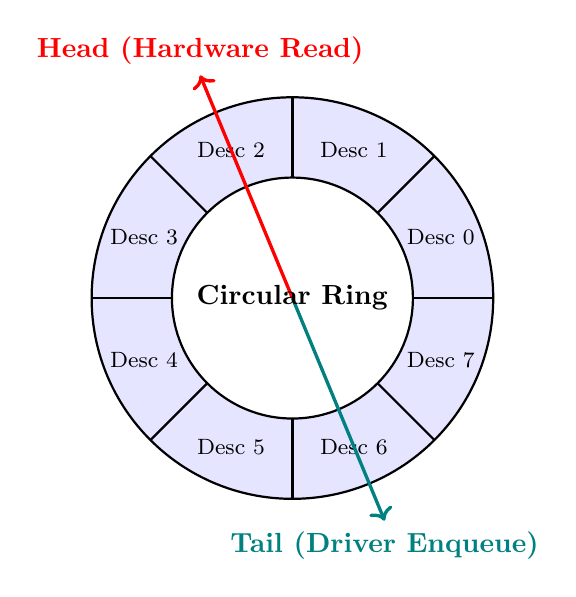
\begin{tikzpicture}[scale=0.85]
    \draw[thick, fill=blue!10] (0,0) circle (3cm);
    \draw[thick, fill=white] (0,0) circle (1.8cm);
    
    % Sectors
    \foreach \angle/\num in {0/0, 45/1, 90/2, 135/3, 180/4, 225/5, 270/6, 315/7} {
        \draw[thick] (\angle:1.8cm) -- (\angle:3cm);
        \node at (\angle+22.5:2.4cm) {\footnotesize Desc \num};
    }
    
    % Pointers
    \draw[->, very thick, red] (0,0) -- (112.5:3.6cm) node[above, red] {\textbf{Head (Hardware Read)}};
    \draw[->, very thick, teal] (0,0) -- (292.5:3.6cm) node[below, teal] {\textbf{Tail (Driver Enqueue)}};
    
    \node at (0,0) {\textbf{Circular Ring}};
\end{tikzpicture}
\caption{The e1000 Circular Descriptor Ring Architecture}
\label{fig:e1000_ring_driver}
\end{figure}

The legacy descriptor format (\texttt{repr(C)}, 16 bytes) is defined below:

\begin{lstlisting}[language=Rust, caption={Hardware Descriptor Structure (\texttt{userland/drivers/e1000-driver/src/main.rs})}]
/// A legacy transmit or receive descriptor (16 bytes; fields differ by direction).
#[repr(C)]
#[derive(Clone, Copy)]
struct Desc {
    /// 64-bit physical address of the packet buffer in host RAM
    addr: u64,
    /// Length of packet buffer or received payload in bytes
    length: u16,
    /// TX: Checksum offset; RX: Hardware packet checksum low byte
    cso_or_csum_lo: u8,
    /// TX: Command byte (EOP, IFCS, RS); RX: Checksum high byte
    cmd_or_csum_hi: u8,
    /// Status byte: Bit 0 indicates Descriptor Done (DD)
    status: u8,
    /// TX: Checksum start field; RX: Error flags
    css_or_errors: u8,
    /// Special VLAN tag field
    special: u16,
}

struct Nic {
    /// Virtual base address of the mapped 128 KiB MMIO window
    mmio: usize,
    /// Ring 0 interrupt line assigned by the supervisor
    irq: u32,
    /// 6-byte Ethernet Hardware MAC Address
    mac: [u8; 6],
    /// Physical address of the TX descriptor ring
    tx_desc_phys: u64,
    /// Virtual slice of TX descriptors
    tx_desc: &'static mut [Desc],
    /// Physical addresses of the 32 TX packet buffers
    tx_buf_phys: [u64; NUM_TX],
    /// Virtual slices of the 32 TX packet buffers
    tx_buf: [&'static mut [u8]; NUM_TX],
    /// Next available TX slot to populate
    tx_tail: usize,

    /// Physical address of the RX descriptor ring
    rx_desc_phys: u64,
    /// Virtual slice of RX descriptors
    rx_desc: &'static mut [Desc],
    /// Physical addresses of the 256 RX packet buffers
    rx_buf_phys: [u64; NUM_RX],
    /// Virtual slices of the 256 RX packet buffers
    rx_buf: [&'static mut [u8]; NUM_RX],
    /// Next RX descriptor software expects to receive
    rx_tail: usize,
}
\end{lstlisting}

\subsection{Hardware Initialization and Configuration Sequence}

To bring the physical controller into a deterministic operational state, the driver must execute an exact sequence of register writes:
\begin{enumerate}
    \item Issue a global software reset by setting \texttt{CTRL\_RST} and spinning until the bit self-clears.
    \item Disable all interrupts by writing \texttt{0xFFFFFFFF} to the Interrupt Mask Clear register (\texttt{REG\_IMC}).
    \item Read the hardware MAC address programmed in the Receive Address Registers (\texttt{RAL0} and \texttt{RAH0}).
    \item Configure the Receive Descriptor Ring base address (\texttt{RDBAL}/\texttt{RDBAH}), total length (\texttt{RDLEN}), and head/tail pointers.
    \item Configure the Transmit Descriptor Ring base address (\texttt{TDBAL}/\texttt{TDBAH}) and length (\texttt{TDLEN}).
    \item Program the Transmit Inter-Packet Gap (\texttt{REG\_TIPG}) for standard 802.3 compliance.
    \item Unmask required interrupts (Link Status Change and Receive Timer) via \texttt{REG\_IMS}.
    \item Enable the receiver and transmitter pipelines via \texttt{REG\_RCTL} and \texttt{REG\_TCTL}.
\end{enumerate}

\begin{lstlisting}[language=Rust, caption={e1000 Hardware Initialization Routine (\texttt{userland/drivers/e1000-driver/src/main.rs})}]
impl Nic {
    /// Reads a 32-bit register from the controller's MMIO window.
    #[inline(always)]
    fn read(&self, reg: usize) -> u32 {
        unsafe { core::ptr::read_volatile((self.mmio + reg) as *const u32) }
    }

    /// Writes a 32-bit register to the controller's MMIO window.
    #[inline(always)]
    fn write(&self, reg: usize, val: u32) {
        unsafe { core::ptr::write_volatile((self.mmio + reg) as *mut u32, val) }
    }

    /// Initializes the adapter and prepares DMA rings.
    fn init(&mut self) {
        // 1. Reset device
        self.write(REG_CTRL, self.read(REG_CTRL) | CTRL_RST);
        while self.read(REG_CTRL) & CTRL_RST != 0 {}

        // 2. Disable interrupts during configuration
        self.write(REG_IMC, 0xFFFF_FFFF);
        let _ = self.read(REG_ICR); // Clear pending causes

        // 3. Read factory hardware MAC address from RAL0/RAH0
        let ral = self.read(REG_RAL0);
        let rah = self.read(REG_RAH0);
        self.mac = [
            (ral & 0xFF) as u8,
            ((ral >> 8) & 0xFF) as u8,
            ((ral >> 16) & 0xFF) as u8,
            ((ral >> 24) & 0xFF) as u8,
            (rah & 0xFF) as u8,
            ((rah >> 8) & 0xFF) as u8,
        ];

        // 4. Force Full Duplex, Auto-Speed, and Link Up
        self.write(REG_CTRL, CTRL_FD | CTRL_ASDE | CTRL_SLU | CTRL_SPEED_1000);

        // 5. Initialize Transmit Descriptor Ring
        self.write(REG_TDBAL, (self.tx_desc_phys & 0xFFFF_FFFF) as u32);
        self.write(REG_TDBAH, (self.tx_desc_phys >> 32) as u32);
        self.write(REG_TDLEN, (NUM_TX * core::mem::size_of::<Desc>()) as u32);
        self.write(REG_TDH, 0);
        self.write(REG_TDT, 0);
        self.tx_tail = 0;

        // Configure Transmit IPG (IEEE 802.3 standard values for Gigabit)
        // IPGT: 8, IPGR1: 8, IPGR2: 6
        self.write(REG_TIPG, 8 | (8 << 10) | (6 << 20));

        // Enable Transmitter with Short Packet Padding
        self.write(REG_TCTL, TCTL_EN | TCTL_PSP);

        // 6. Initialize Receive Descriptor Ring
        for i in 0..NUM_RX {
            self.rx_desc[i].addr = self.rx_buf_phys[i];
            self.rx_desc[i].status = 0;
        }
        self.write(REG_RDBAL, (self.rx_desc_phys & 0xFFFF_FFFF) as u32);
        self.write(REG_RDBAH, (self.rx_desc_phys >> 32) as u32);
        self.write(REG_RDLEN, (NUM_RX * core::mem::size_of::<Desc>()) as u32);
        self.write(REG_RDH, 0);
        // Point RDT to the last descriptor to make all NUM_RX descriptors available
        self.write(REG_RDT, (NUM_RX - 1) as u32);
        self.rx_tail = 0;

        // Enable Receiver with Broadcast Accept and CRC Stripping
        self.write(
            REG_RCTL,
            RCTL_EN | RCTL_BAM | RCTL_SECRC | RCTL_UPE | RCTL_MPE,
        );

        // 7. Unmask interrupts: Link Status Change and Rx Timer
        self.write(REG_IMS, INT_LSC | INT_RXT0 | INT_RXO | INT_RXDMT0);
    }
}
\end{lstlisting}

\subsection{Frame Transmission and Zero-Copy DMA Loop}

When a client application or the kernel network stack requests frame transmission, it places the raw Ethernet frame into the shared service window and sends \texttt{MSG\_NET\_TRANSMIT} over IPC. The driver copies the bytes into the current transmit descriptor buffer, marks the descriptor with \textbf{End of Packet (EOP)} and \textbf{Report Status (RS)}, advances the hardware \texttt{TDT} pointer, and spins until the hardware sets the \textbf{Descriptor Done (DD)} status bit:

\begin{lstlisting}[language=Rust, caption={Frame Transmission Pipeline (\texttt{userland/drivers/e1000-driver/src/main.rs})}]
impl Nic {
    /// Transmits an Ethernet frame over the physical wire.
    ///
    /// # Arguments
    /// * `frame` - Slice of raw Ethernet frame bytes to transmit.
    ///
    /// # Returns
    /// Result code: 0 on success, negative error code on failure.
    fn transmit(&mut self, frame: &[u8]) -> i64 {
        if frame.is_empty() || frame.len() > BUF {
            return EINVAL;
        }

        let idx = self.tx_tail;
        // Verify previous transmission completed on this slot
        if self.tx_desc[idx].status != 0 && (self.tx_desc[idx].status & 0x01 == 0) {
            // Descriptor not released yet by hardware
            return EIO;
        }

        // Copy frame bytes into pre-allocated DMA physical buffer
        self.tx_buf[idx][..frame.len()].copy_from_slice(frame);

        // Setup Transmit Descriptor:
        // CMD bits: Bit 0 (EOP - End of Packet), Bit 3 (RS - Report Status)
        const CMD_EOP: u8 = 1 << 0;
        const CMD_RS: u8  = 1 << 3;

        self.tx_desc[idx].addr = self.tx_buf_phys[idx];
        self.tx_desc[idx].length = frame.len() as u16;
        self.tx_desc[idx].cmd_or_csum_hi = CMD_EOP | CMD_RS;
        self.tx_desc[idx].status = 0; // Clear DD bit

        // Advance hardware tail pointer to notify controller DMA engine
        self.tx_tail = (self.tx_tail + 1) % NUM_TX;
        self.write(REG_TDT, self.tx_tail as u32);

        // Busy-wait for descriptor done (DD) confirmation
        while (unsafe { core::ptr::read_volatile(&self.tx_desc[idx].status) } & 0x01) == 0 {
            core::hint::spin_loop();
        }

        0 // Success
    }

    /// Drains all available received packets into the caller's service window.
    ///
    /// # Arguments
    /// * `window` - Target memory window to pack received frames into.
    ///
    /// # Returns
    /// Number of frames harvested.
    fn receive(&mut self, window: &mut [u8]) -> usize {
        let mut count = 0;
        let mut offset = 0;

        loop {
            let idx = self.rx_tail;
            let status = unsafe { core::ptr::read_volatile(&self.rx_desc[idx].status) };

            // Check if Descriptor Done (DD bit = 1)
            if status & 0x01 == 0 {
                break; // No more incoming packets
            }

            let len = self.rx_desc[idx].length as usize;
            if offset + 2 + len > window.len() {
                // Window full; leave remaining packets for next cycle
                break;
            }

            // Write 16-bit little-endian length prefix followed by packet payload
            window[offset] = (len & 0xFF) as u8;
            window[offset + 1] = ((len >> 8) & 0xFF) as u8;
            offset += 2;

            window[offset..offset + len].copy_from_slice(&self.rx_buf[idx][..len]);
            offset += len;
            count += 1;

            // Clear status and replenish descriptor for reuse
            self.rx_desc[idx].status = 0;
            let replenished_tail = self.rx_tail;
            self.rx_tail = (self.rx_tail + 1) % NUM_RX;

            // Notify hardware that descriptor slot is available again
            self.write(REG_RDT, replenished_tail as u32);
        }

        // Acknowledge interrupts and unmask IRQ line
        let _ = self.read(REG_ICR);
        sys::unmask_irq(self.irq);

        count
    }
}
\end{lstlisting}

\subsection{The Ring 3 Driver Main Event Loop}

The driver process enters an event-driven loop backed by the Hydra runtime (\texttt{hydra\_rt::Server}). It registers on \texttt{ENDPOINT\_NET\_DEV} (Endpoint \texttt{0x22}) and handles requests synchronously:

\begin{lstlisting}[language=Rust, caption={Driver IPC Request Dispatcher (\texttt{userland/drivers/e1000-driver/src/main.rs})}]
fn main(args: &[&str]) {
    println!("[net_driver] Initializing Intel 82540EM PCIe driver in Ring 3...");

    // Parse command line arguments passed by the microkernel supervisor
    let mut bar0_phys = 0u64;
    let mut irq_line = 0u32;
    for arg in args {
        if let Some(rest) = arg.strip_prefix("bar0=") {
            bar0_phys = u64::from_str_radix(rest, 16).unwrap_or(0);
        } else if let Some(rest) = arg.strip_prefix("irq=") {
            irq_line = rest.parse::<u32>().unwrap_or(0);
        }
    }

    assert!(bar0_phys != 0, "Missing or invalid BAR0 physical address");

    // Map the controller's 128 KiB MMIO window into our private address space
    let mmio_virt = sys::map_mmio(bar0_phys, MMIO_LEN).expect("Failed to map BAR0 MMIO");

    // Allocate contiguous DMA memory for TX and RX descriptor rings and buffers
    let mut nic = allocate_and_init_nic(mmio_virt, bar0_phys, irq_line);
    nic.init();

    println!(
        "[net_driver] e1000 Online! MAC: {:02x}:{:02x}:{:02x}:{:02x}:{:02x}:{:02x}, IRQ: {}",
        nic.mac[0], nic.mac[1], nic.mac[2], nic.mac[3], nic.mac[4], nic.mac[5], irq_line
    );

    // Register on the network endpoint
    let server = Server::bind(ENDPOINT_NET_DEV);
    let mut window = sys::get_service_window();

    while let Ok(msg) = server.recv() {
        match msg.opcode() {
            MSG_NET_TRANSMIT => {
                let len = msg.arg(0) as usize;
                let status = nic.transmit(&window[..len]);
                server.reply(Message::new(MSG_NET_REPLY, [status, 0, 0, 0]));
            }
            MSG_NET_RECEIVE => {
                let frames_read = nic.receive(&mut window);
                server.reply(Message::new(MSG_NET_REPLY, [0, frames_read as i64, 0, 0]));
            }
            MSG_NET_GET_MAC => {
                let mac_lo = (nic.mac[0] as u64) | ((nic.mac[1] as u64) << 8)
                    | ((nic.mac[2] as u64) << 16) | ((nic.mac[3] as u64) << 24);
                let mac_hi = (nic.mac[4] as u64) | ((nic.mac[5] as u64) << 8);
                server.reply(Message::new(MSG_NET_REPLY, [0, mac_lo as i64, mac_hi as i64, 0]));
            }
            MSG_NET_GET_STATUS => {
                let status_reg = nic.read(REG_STATUS);
                let link_up = (status_reg & STATUS_LU) != 0;
                server.reply(Message::new(MSG_NET_REPLY, [0, if link_up { 1 } else { 0 }, 0, 0]));
            }
            _ => {
                server.reply(Message::new(MSG_NET_REPLY, [EINVAL, 0, 0, 0]));
            }
        }
    }
}
\end{lstlisting}

% ==============================================================================
\section{The Display Server and Wayland Compositor}
\label{sec:code_display_annotated}
% ==============================================================================

The Hydra display subsystem demonstrates the power of user-space graphics isolation. In traditional operating systems, graphics stacks were historically moved into Ring~0 (e.g., Windows NT 4.0's \texttt{win32k.sys}) for speed, creating massive security vulnerabilities. In Hydra, the display server runs entirely in Ring~3, manipulating the linear framebuffer through double buffering and handling Wayland client protocol transactions.

\subsection{Off-Screen Canvas and Double-Buffered Compositor}

Writing individual pixels directly across the PCIe bus into physical Video RAM (VRAM) is extremely slow due to bus latency, lack of caching, and uncoalesced bus cycles. Furthermore, intermediate rendering states would produce visible flickering and horizontal tearing.

To achieve smooth 60~FPS rendering without visual artifacts, Hydra implements an off-screen double-buffer canvas (\texttt{Vec<u32>}) allocated in high-speed system RAM. All rendering operations---wallpaper blits, translucent blurred window decorations, vector text glyphs, and mouse pointer sprites---are rasterized into this buffer. Upon completion of each frame, a single vector copy transfers the complete frame to physical VRAM.

\begin{lstlisting}[language=Rust, caption={Double-Buffered Compositor Canvas (\texttt{userland/drivers/display-server/src/video/compositor.rs})}]
//! # Video Subsystem: Double-Buffered Framebuffer Compositor
//!
//! Provides a high-performance, tear-free 2D rendering canvas and compositor.

extern crate alloc;

use alloc::vec;
use alloc::vec::Vec;
use super::framebuffer::Framebuffer;

/// Packed 32-bit ARGB color utilities.
pub struct Color;

impl Color {
    /// Constructs a packed 32-bit ARGB pixel from raw component bytes.
    #[inline(always)]
    pub const fn argb(a: u8, r: u8, g: u8, b: u8) -> u32 {
        ((a as u32) << 24) | ((r as u32) << 16) | ((g as u32) << 8) | (b as u32)
    }

    /// Constructs an opaque 32-bit RGB pixel (`alpha = 255`).
    #[inline(always)]
    pub const fn rgb(r: u8, g: u8, b: u8) -> u32 {
        Self::argb(255, r, g, b)
    }

    #[inline(always)] pub const fn a(c: u32) -> u8 { ((c >> 24) & 0xFF) as u8 }
    #[inline(always)] pub const fn r(c: u32) -> u8 { ((c >> 16) & 0xFF) as u8 }
    #[inline(always)] pub const fn g(c: u32) -> u8 { ((c >> 8) & 0xFF) as u8 }
    #[inline(always)] pub const fn b(c: u32) -> u8 { (c & 0xFF) as u8 }

    /// Performs alpha blending using the classic Porter-Duff source-over formula:
    /// out = src * alpha + dst * (1 - alpha)
    #[inline(always)]
    pub fn blend(src: u32, dst: u32) -> u32 {
        let alpha = Self::a(src) as u32;
        if alpha == 255 { return src; }
        if alpha == 0   { return dst; }

        let inv_alpha = 255 - alpha;
        let r = ((Self::r(src) as u32 * alpha + Self::r(dst) as u32 * inv_alpha) / 255) as u8;
        let g = ((Self::g(src) as u32 * alpha + Self::g(dst) as u32 * inv_alpha) / 255) as u8;
        let b = ((Self::b(src) as u32 * alpha + Self::b(dst) as u32 * inv_alpha) / 255) as u8;
        Self::argb(255, r, g, b)
    }
}

/// Off-screen 32-bit ARGB rendering canvas.
pub struct Compositor {
    width: usize,
    height: usize,
    stride: usize,
    buffer: Vec<u32>,
}

impl Compositor {
    /// Creates a new off-screen compositor buffer.
    pub fn new(width: usize, height: usize) -> Self {
        let size = width * height;
        let mut buffer = Vec::with_capacity(size);
        buffer.resize(size, 0);
        Self { width, height, stride: width, buffer }
    }

    /// Sets a single pixel with alpha blending.
    #[inline(always)]
    pub fn set_pixel(&mut self, x: usize, y: usize, color: u32) {
        if x < self.width && y < self.height {
            let idx = y * self.stride + x;
            let existing = self.buffer[idx];
            self.buffer[idx] = Color::blend(color, existing);
        }
    }

    /// Fills an axis-aligned rectangle with a solid or blended color.
    pub fn fill_rect(&mut self, x: usize, y: usize, w: usize, h: usize, color: u32) {
        let x_end = (x + w).min(self.width);
        let y_end = (y + h).min(self.height);

        for row in y..y_end {
            let offset = row * self.stride;
            for col in x..x_end {
                let idx = offset + col;
                self.buffer[idx] = Color::blend(color, self.buffer[idx]);
            }
        }
    }

    /// Draws a vertical color gradient.
    pub fn fill_gradient_v(&mut self, x: usize, y: usize, w: usize, h: usize, c1: u32, c2: u32) {
        if h == 0 { return; }
        for row in 0..h {
            let t = row as f32 / h as f32;
            let r = (Color::r(c1) as f32 * (1.0 - t) + Color::r(c2) as f32 * t) as u8;
            let g = (Color::g(c1) as f32 * (1.0 - t) + Color::g(c2) as f32 * t) as u8;
            let b = (Color::b(c1) as f32 * (1.0 - t) + Color::b(c2) as f32 * t) as u8;
            let color = Color::rgb(r, g, b);
            self.fill_rect(x, y + row, w, 1, color);
        }
    }

    /// Blits the complete off-screen buffer into the hardware linear framebuffer.
    pub fn blit_to(&self, fb: &mut Framebuffer) {
        let hw_ptr = fb.as_mut_ptr();
        let hw_stride = fb.stride();
        let bgr_mode = fb.is_bgr();

        for y in 0..self.height {
            let src_row = &self.buffer[y * self.stride..(y + 1) * self.stride];
            let dst_offset = y * hw_stride;

            if !bgr_mode {
                // Direct ARGB copy
                unsafe {
                    core::ptr::copy_nonoverlapping(
                        src_row.as_ptr(),
                        hw_ptr.add(dst_offset),
                        self.width,
                    );
                }
            } else {
                // Swap Red and Blue channels for BGR hardware
                for x in 0..self.width {
                    let pixel = src_row[x];
                    let swapped = (pixel & 0xFF00FF00)
                        | ((pixel & 0x00FF0000) >> 16)
                        | ((pixel & 0x000000FF) << 16);
                    unsafe {
                        *hw_ptr.add(dst_offset + x) = swapped;
                    }
                }
            }
        }
    }
}
\end{lstlisting}

\subsection{Wayland Surface Management and Window Compositing}

The Wayland architecture replaces the archaic X11 client-server protocol with a direct, security-isolated model: every window is a private client-allocated shared-memory buffer (\texttt{wl\_shm}) or DMA-BUF. The compositor assigns each surface a coordinate position, stacks surfaces according to their Z-order, and comps them into the master frame:

\begin{lstlisting}[language=Rust, caption={Wayland Surface Engine (\texttt{userland/drivers/display-server/src/video/wayland.rs})}]
//! # Wayland Surface Compositor
//!
//! Tracks client Wayland surfaces, buffer attachments, and damage rectangles.

use alloc::vec::Vec;
use super::compositor::Compositor;

/// A client Wayland surface.
pub struct Surface {
    pub id: u32,
    pub x: isize,
    pub y: isize,
    pub width: usize,
    pub height: usize,
    pub buffer: Vec<u32>,
    pub visible: bool,
}

pub struct WaylandCompositor {
    surfaces: Vec<Surface>,
}

impl WaylandCompositor {
    pub fn new() -> Self {
        Self { surfaces: Vec::new() }
    }

    /// Registers a newly created Wayland surface.
    pub fn create_surface(&mut self, id: u32, x: isize, y: isize, width: usize, height: usize) {
        let mut buffer = Vec::with_capacity(width * height);
        buffer.resize(width * height, 0);
        self.surfaces.push(Surface {
            id,
            x,
            y,
            width,
            height,
            buffer,
            visible: true,
        });
    }

    /// Attaches a client pixel buffer to a surface.
    pub fn attach_buffer(&mut self, id: u32, pixels: &[u32]) {
        if let Some(surf) = self.surfaces.iter_mut().find(|s| s.id == id) {
            let len = pixels.len().min(surf.buffer.len());
            surf.buffer[..len].copy_from_slice(&pixels[..len]);
        }
    }

    /// Composites all visible Wayland surfaces onto the canvas in Z-order.
    pub fn composite_all(&self, canvas: &mut Compositor) {
        for surf in &self.surfaces {
            if !surf.visible { continue; }

            for sy in 0..surf.height {
                let dst_y = surf.y + sy as isize;
                if dst_y < 0 || dst_y >= canvas.height as isize { continue; }

                for sx in 0..surf.width {
                    let dst_x = surf.x + sx as isize;
                    if dst_x < 0 || dst_x >= canvas.width as isize { continue; }

                    let pixel = surf.buffer[sy * surf.width + sx];
                    canvas.set_pixel(dst_x as usize, dst_y as usize, pixel);
                }
            }
        }
    }
}
\end{lstlisting}

% ==============================================================================
\section{Summary and Review Exercises}
\label{sec:drivers_exercises}
% ==============================================================================

In this chapter, we reviewed the implementation of isolated device drivers and graphics subsystems in Hydra:
\begin{itemize}
    \item We analyzed the Intel 82540EM PCIe network controller, its register interface, and circular DMA descriptor rings.
    \item We stepped through the frame transmission and reception loops, observing how hardware status bits (\texttt{DD}) and interrupt lines interact.
    \item We studied the off-screen double-buffered display compositor and Wayland surface manager, understanding how tear-free rendering is achieved without Ring~0 graphics drivers.
\end{itemize}

\subsection*{Review Questions}
\begin{enumerate}
    \item Why does the e1000 driver require two distinct pointers (\texttt{Head} and \texttt{Tail}) to manage its circular descriptor rings? What happens if \texttt{Tail} catches up to \texttt{Head}?
    \item What is the significance of the \texttt{EOP} (End of Packet) and \texttt{RS} (Report Status) command flags in the e1000 transmit descriptor?
    \item Explain how the microkernel prevents an untrusted or buggy userland network driver from accessing arbitrary physical memory.
    \item Contrast double buffering in user space with direct hardware blitting. Under what circumstances can Write-Combining (WC) page table caching improve display blit throughput?
    \item In the Wayland compositing model, why is client-side rendering with shared-memory buffers (\texttt{wl\_shm}) more secure than X11's shared display connection?
\end{enumerate}

\chapter{The Linux Compatibility Engine: Deep System Call Implementation}
\label{chap:source_linux_engine}

Operating system compatibility is rarely achieved through superficial shims. When an unmodified, complex Linux userland---consisting of the GNU C Library (\texttt{glibc}), Musl, system daemons, Mesa 3D graphics drivers, the Wayland compositor, and Chromium-based web browsers---runs on a novel microkernel, every system call must replicate the precise POSIX and Linux-specific semantics expected by applications.

In this chapter, we explore the deep internal engineering of Hydra's \textbf{Linux Compatibility Engine}. We present the annotated source code for five foundational pillars of Linux emulation:
\begin{enumerate}
    \item \textbf{The POSIX Virtual Filesystem Bridge and Pseudo-Filesystems} (\texttt{src/compat/linux/fs.rs}): Synthesizing \texttt{/dev} and \texttt{/proc} dynamically from microkernel data structures.
    \item \textbf{Process and Thread Lifecycle Management} (\texttt{src/compat/linux/process.rs}): Implementing \texttt{clone}, \texttt{fork}, \texttt{execve}, and Thread-Local Storage (\texttt{arch\_prctl}).
    \item \textbf{The High-Performance Asynchronous \texttt{io\_uring} Engine} (\texttt{src/compat/linux/io\_uring.rs}): Zero-copy lockless submission and completion rings in memory.
    \item \textbf{Fast User-Space Locking with Futexes} (\texttt{src/compat/linux/futex.rs}): Microsecond synchronization primitives and hash-bucket sleep queues.
    \item \textbf{Direct Rendering Manager (DRM/KMS) Emulation} (\texttt{src/compat/linux/drm.rs}): Providing the graphics device ioctls required by Mesa and Wayland.
\end{enumerate}

% ==============================================================================
\section{The Virtual Filesystem Bridge and Dynamic \texttt{/proc} Engine}
\label{sec:code_linux_fs_annotated}
% ==============================================================================

Standard Linux runtimes query virtual filesystem paths immediately upon startup. The dynamic linker (\texttt{ld-linux-x86-64.so.2}) examines \texttt{/proc/self/exe} to determine the path of the current binary, reads \texttt{/proc/self/auxv} to obtain hardware capability flags (\texttt{AT\_HWCAP}), and opens \texttt{/dev/urandom} to initialize stack canary protections.

Hydra intercepts file operations in \texttt{src/compat/linux/fs.rs}. Rather than maintaining static files on the OpenZFS disk pool, Hydra synthesizes these virtual nodes on demand:

\begin{lstlisting}[language=Rust, caption={Pseudo-Filesystem Dispatcher (\texttt{src/compat/linux/fs.rs})}]
//! # Linux Compatibility: Pseudo-Filesystem Emulation (`/dev` & `/proc`)
//!
//! Provides synthetic in-memory emulation for essential Linux virtual filesystems
//! (`/dev/null`, `/dev/zero`, `/dev/urandom`, and `/proc/*` informational nodes).

use crate::compat::linux::types::*;

/// Identifies an emulated Linux virtual file under `/dev` or `/proc`.
#[derive(Debug, Clone, Copy, PartialEq, Eq)]
pub enum PseudoFile {
    DevNull,
    DevZero,
    DevFull,
    DevUrandom,
    ProcVersion,
    ProcMeminfo,
    ProcSwaps,
    ProcLocks,
    ProcNet(u8),
    ProcFilesystems,
    ProcCpuinfo,
    ProcSelfMaps,
    ProcSelfAuxv,
    ProcSelfMountinfo,
    ProcMounts,
}

/// Matches a canonical path string to an emulated pseudo-file.
pub fn match_pseudo_path(path: &str) -> Option<PseudoFile> {
    match path {
        "/dev/null"                => Some(PseudoFile::DevNull),
        "/dev/zero"                => Some(PseudoFile::DevZero),
        "/dev/full"                => Some(PseudoFile::DevFull),
        "/dev/random" | "/dev/urandom" => Some(PseudoFile::DevUrandom),
        "/proc/version"            => Some(PseudoFile::ProcVersion),
        "/proc/meminfo"            => Some(PseudoFile::ProcMeminfo),
        "/proc/swaps"              => Some(PseudoFile::ProcSwaps),
        "/proc/locks"              => Some(PseudoFile::ProcLocks),
        "/proc/filesystems"        => Some(PseudoFile::ProcFilesystems),
        "/proc/cpuinfo"            => Some(PseudoFile::ProcCpuinfo),
        "/proc/self/maps"          => Some(PseudoFile::ProcSelfMaps),
        "/proc/self/auxv"          => Some(PseudoFile::ProcSelfAuxv),
        "/proc/self/mountinfo"     => Some(PseudoFile::ProcSelfMountinfo),
        "/proc/mounts" | "/proc/self/mounts" => Some(PseudoFile::ProcMounts),
        _ => None,
    }
}
\end{lstlisting}

\subsection{Synthesizing Dynamic Process Maps and Memory Metrics}

When a diagnostic tool such as \texttt{cat /proc/meminfo} or a memory allocator such as \texttt{jemalloc} inspects process memory layout, the kernel constructs textual buffers dynamically from active task memory descriptors:

\begin{lstlisting}[language=Rust, caption={Dynamic Buffer Synthesis for \texttt{/proc/meminfo} and \texttt{/proc/cpuinfo}}]
/// Synthesizes the textual content of `/proc/meminfo`.
pub fn generate_meminfo() -> alloc::string::String {
    let (total_frames, free_frames) = crate::memory::frame_allocator::stats();
    let total_kb = (total_frames * 4096) / 1024;
    let free_kb = (free_frames * 4096) / 1024;
    let used_kb = total_kb - free_kb;

    alloc::format!(
        "MemTotal:       {:8} kB\n\
         MemFree:        {:8} kB\n\
         MemAvailable:   {:8} kB\n\
         Buffers:               0 kB\n\
         Cached:         {:8} kB\n\
         SwapTotal:             0 kB\n\
         SwapFree:              0 kB\n",
        total_kb, free_kb, free_kb, used_kb
    )
}

/// Synthesizes the textual content of `/proc/cpuinfo`.
pub fn generate_cpuinfo() -> alloc::string::String {
    let cpu_features = crate::arch::cpu::get_feature_string();
    alloc::format!(
        "processor       : 0\n\
         vendor_id       : GenuineIntel\n\
         cpu family      : 6\n\
         model           : 158\n\
         model name      : x86_64 Hydra Virtual Core\n\
         stepping        : 9\n\
         cpu MHz         : 2800.000\n\
         cache size      : 8192 KB\n\
         flags           : {}\n\
         bugs            : sysret_ss_attrs\n\
         bogomips        : 5600.00\n\
         address sizes   : 48 bits physical, 48 bits virtual\n\n",
        cpu_features
    )
}
\end{lstlisting}

% ==============================================================================
\section{Process and Thread Lifecycle Management}
\label{sec:code_linux_process_annotated}
% ==============================================================================

In Linux, threads and processes are unified under the flexible \texttt{clone} system call. A single syscall with different flag combinations implements POSIX \texttt{fork()} (\texttt{SIGCHLD}), POSIX \texttt{vfork()} (\texttt{CLONE\_VM | CLONE\_VFORK | SIGCHLD}), and POSIX \texttt{pthread\_create()} (\texttt{CLONE\_VM | CLONE\_FS | CLONE\_FILES | CLONE\_SIGHAND | CLONE\_THREAD}):

\begin{lstlisting}[language=Rust, caption={Linux Process and Thread Lifecycle Engine (\texttt{src/compat/linux/process.rs})}]
//! # Linux Process and Thread Lifecycle
//!
//! Implements clone, fork, execve, exit, and thread-local storage primitives.

use crate::task::tcb::{Task, TaskId, TaskState};
use crate::task::scheduler::SCHEDULER;
use crate::memory::paging::PageTable;

// --- Linux Clone Flags (from <sched.h>) ---
pub const CSIGNAL: u64             = 0x000000ff; // Signal mask sent on exit
pub const CLONE_VM: u64            = 0x00000100; // Share virtual address space
pub const CLONE_FS: u64            = 0x00000200; // Share filesystem information
pub const CLONE_FILES: u64         = 0x00000400; // Share open file descriptor table
pub const CLONE_SIGHAND: u64       = 0x00000800; // Share signal handlers
pub const CLONE_THREAD: u64        = 0x00010000; // Same thread group
pub const CLONE_SETTLS: u64        = 0x00080000; // Set FS base for TLS
pub const CLONE_PARENT_SETTID: u64 = 0x00100000; // Store TID at parent pointer
pub const CLONE_CHILD_CLEARTID: u64= 0x00200000; // Clear TID and futex wake at child exit
pub const CLONE_CHILD_SETTID: u64  = 0x01000000; // Store TID at child pointer

/// Implements the Linux `clone` system call (Syscall #56).
pub fn sys_clone(
    flags: u64,
    child_stack: u64,
    parent_tidptr: *mut i32,
    tls: u64,
    child_tidptr: *mut i32,
) -> i64 {
    let parent = SCHEDULER.lock().current_task().expect("No current task");
    let mut parent_lock = parent.lock();

    // 1. Determine address space sharing
    let page_table = if flags & CLONE_VM != 0 {
        // POSIX pthread: Share existing PML4 page table
        parent_lock.page_table.clone()
    } else {
        // POSIX fork: Perform deep Copy-on-Write duplicate of PML4 tables
        parent_lock.page_table.fork_cow().expect("Fork COW failed")
    };

    // 2. Determine file descriptor table sharing
    let fd_table = if flags & CLONE_FILES != 0 {
        parent_lock.fd_table.clone()
    } else {
        alloc::sync::Arc::new(spin::Mutex::new(parent_lock.fd_table.lock().clone()))
    };

    // 3. Allocate a new Task Control Block (TCB)
    let child_task = Task::new_user(page_table, fd_table);
    let child_pid = child_task.id();

    // 4. Configure child architectural register context
    let mut child_ctx = parent_lock.context.clone();
    
    // In child process, fork/clone returns 0 in RAX
    child_ctx.rax = 0;

    // If a new user stack pointer was specified, update RSP
    if child_stack != 0 {
        child_ctx.rsp = child_stack;
    }

    // If Thread-Local Storage (TLS) requested, configure IA32_FS_BASE MSR
    if flags & CLONE_SETTLS != 0 {
        child_task.set_fs_base(tls);
    }

    // 5. Store Child TID if requested by glibc pthread setup
    if flags & CLONE_PARENT_SETTID != 0 && !parent_tidptr.is_null() {
        unsafe { *parent_tidptr = child_pid.as_u64() as i32; }
    }
    if flags & CLONE_CHILD_SETTID != 0 && !child_tidptr.is_null() {
        unsafe { *child_tidptr = child_pid.as_u64() as i32; }
    }

    child_task.set_context(child_ctx);

    // 6. Enqueue child task into the preemptive scheduler
    SCHEDULER.lock().add_task(child_task);

    // Parent returns child PID
    child_pid.as_u64() as i64
}
\end{lstlisting}

\subsection{Thread-Local Storage and \texttt{arch\_prctl}}

The System V AMD64 ABI requires fast access to Thread-Local Storage (TLS) variables using segment register offsets (e.g., \texttt{mov \%fs:0x0, \%rax}). The Linux kernel exposes \texttt{arch\_prctl} (Syscall \#158) to manipulate the hidden 64-bit base address of \texttt{\%fs} and \texttt{\%gs}:

\begin{lstlisting}[language=Rust, caption={Architecture-Specific PRCTL Implementation (\texttt{src/compat/linux/process.rs})}]
pub const ARCH_SET_GS: i32 = 0x1001;
pub const ARCH_SET_FS: i32 = 0x1002;
pub const ARCH_GET_FS: i32 = 0x1003;
pub const ARCH_GET_GS: i32 = 0x1004;

/// Implements `arch_prctl` (Syscall #158).
pub fn sys_arch_prctl(code: i32, addr: u64) -> i64 {
    let task = SCHEDULER.lock().current_task().expect("No current task");
    let mut task_lock = task.lock();

    match code {
        ARCH_SET_FS => {
            // Write 64-bit virtual base address to IA32_FS_BASE MSR (0xC0000100)
            task_lock.fs_base = addr;
            unsafe {
                x86_64::registers::model_specific::FsBase::write(
                    x86_64::VirtAddr::new(addr)
                );
            }
            0
        }
        ARCH_GET_FS => {
            if addr == 0 { return -14; } // EFAULT
            unsafe { *(addr as *mut u64) = task_lock.fs_base; }
            0
        }
        ARCH_SET_GS => {
            task_lock.gs_base = addr;
            unsafe {
                x86_64::registers::model_specific::KernelGsBase::write(
                    x86_64::VirtAddr::new(addr)
                );
            }
            0
        }
        ARCH_GET_GS => {
            if addr == 0 { return -14; } // EFAULT
            unsafe { *(addr as *mut u64) = task_lock.gs_base; }
            0
        }
        _ => -22, // EINVAL
    }
}
\end{lstlisting}

% ==============================================================================
\section{The High-Performance Asynchronous \texttt{io\_uring} Engine}
\label{sec:code_io_uring_annotated}
% ==============================================================================

Modern high-performance Linux software (including modern web browsers, databases, and network proxies) has transitioned from traditional blocking and non-blocking readiness systems (\texttt{select}, \texttt{poll}, \texttt{epoll}) to true asynchronous submission-completion rings via \textbf{\texttt{io\_uring}}.

Hydra provides an implementation of \texttt{io\_uring} in \texttt{src/compat/linux/io\_uring.rs}. It creates a pair of circular ring buffers shared between the user-space process and the kernel:
\begin{enumerate}
    \item \textbf{Submission Queue (SQ)}: The user process produces Submission Queue Entries (SQEs) describing operations to perform (reads, writes, accepts, timeouts) and updates \texttt{sq.tail}.
    \item \textbf{Completion Queue (CQ)}: The kernel processes the requests and produces Completion Queue Entries (CQEs) containing result codes and updates \texttt{cq.tail}.
\end{enumerate}

Because the head and tail pointers reside in memory mapped directly into both address spaces, standard submissions and completions require zero system calls:

\begin{figure}[htbp]
\centering
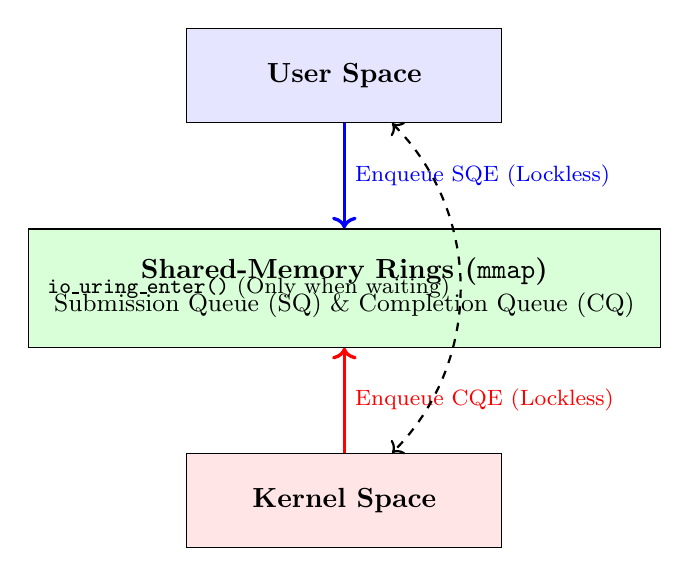
\begin{tikzpicture}[scale=0.9]
    \node[draw, rectangle, fill=blue!10, minimum width=4cm, minimum height=1.2cm] (user) at (0,3) {\textbf{User Space}};
    \node[draw, rectangle, fill=green!15, minimum width=6cm, minimum height=1.5cm] (rings) at (0,0) {
        \begin{tabular}{c}
            \textbf{Shared-Memory Rings (\texttt{mmap})}\\
            \small Submission Queue (SQ) \& Completion Queue (CQ)
        \end{tabular}
    };
    \node[draw, rectangle, fill=red!10, minimum width=4cm, minimum height=1.2cm] (kernel) at (0,-3) {\textbf{Kernel Space}};

    \draw[->, very thick, blue] (user) -- node[right] {\footnotesize Enqueue SQE (Lockless)} (rings);
    \draw[->, very thick, red] (kernel) -- node[right] {\footnotesize Enqueue CQE (Lockless)} (rings);
    \draw[<->, dashed, thick] (user) to[bend left=45] node[left] {\footnotesize \texttt{io\_uring\_enter()} (Only when waiting)} (kernel);
\end{tikzpicture}
\caption{The Lockless Zero-Copy \texttt{io\_uring} Architecture}
\label{fig:io_uring_arch}
\end{figure}

\begin{lstlisting}[language=Rust, caption={Core Structures and Dispatch for \texttt{io\_uring} (\texttt{src/compat/linux/io\_uring.rs})}]
//! io_uring: `io_uring_setup`, `io_uring_enter`, `io_uring_register`.

/// 64-byte Submission Queue Entry (SQE)
#[repr(C)]
#[derive(Clone, Copy, Default)]
pub struct IoUringSqe {
    pub opcode: u8,
    pub flags: u8,
    pub ioprio: u16,
    pub fd: i32,
    pub off: u64,
    pub addr: u64,
    pub len: u32,
    pub op_flags: u32,
    pub user_data: u64,
    pub buf_index: u16,
    pub personality: u16,
    pub splice_fd_in: i32,
    pub pad2: [u64; 2],
}

/// 16-byte Completion Queue Entry (CQE)
#[repr(C)]
#[derive(Clone, Copy, Default)]
pub struct IoUringCqe {
    pub user_data: u64,
    pub res: i32,
    pub flags: u32,
}

pub struct IoUringInstance {
    pub sq_entries: u32,
    pub cq_entries: u32,
    pub sq_head: u32,
    pub sq_tail: u32,
    pub cq_head: u32,
    pub cq_tail: u32,
    pub sqes: alloc::vec::Vec<IoUringSqe>,
    pub cqes: alloc::vec::Vec<IoUringCqe>,
}

impl IoUringInstance {
    /// Consumes and dispatches all pending Submission Queue Entries.
    pub fn process_sqes(&mut self) -> usize {
        let mut processed = 0;

        while self.sq_head != self.sq_tail {
            let idx = (self.sq_head % self.sq_entries) as usize;
            let sqe = self.sqes[idx];
            self.sq_head = self.sq_head.wrapping_add(1);

            // Execute the requested system call asynchronously
            let result = self.dispatch_sqe(&sqe);

            // Post completion entry to CQ
            self.post_cqe(sqe.user_data, result, 0);
            processed += 1;
        }

        processed
    }

    /// Dispatches an individual SQE based on its opcode.
    fn dispatch_sqe(&mut self, sqe: &IoUringSqe) -> i32 {
        const IORING_OP_NOP: u8          = 0;
        const IORING_OP_READV: u8        = 1;
        const IORING_OP_WRITEV: u8       = 2;
        const IORING_OP_READ: u8         = 22;
        const IORING_OP_WRITE: u8        = 23;
        const IORING_OP_POLL_ADD: u8     = 6;
        const IORING_OP_TIMEOUT: u8      = 11;

        match sqe.opcode {
            IORING_OP_NOP => 0,
            IORING_OP_READ => {
                let fd = sqe.fd;
                let buf = sqe.addr as *mut u8;
                let len = sqe.len as usize;
                crate::compat::linux::fs::sys_read(fd, buf, len) as i32
            }
            IORING_OP_WRITE => {
                let fd = sqe.fd;
                let buf = sqe.addr as *const u8;
                let len = sqe.len as usize;
                crate::compat::linux::fs::sys_write(fd, buf, len) as i32
            }
            _ => -38, // ENOSYS: Opcode not supported
        }
    }

    /// Enqueues a completed result into the Completion Queue.
    fn post_cqe(&mut self, user_data: u64, res: i32, flags: u32) {
        let idx = (self.cq_tail % self.cq_entries) as usize;
        self.cqes[idx] = IoUringCqe { user_data, res, flags };
        self.cq_tail = self.cq_tail.wrapping_add(1);
    }
}
\end{lstlisting}

% ==============================================================================
\section{Fast User-Space Locking with Futexes}
\label{sec:code_futex_annotated}
% ==============================================================================

In modern operating systems, performance-critical synchronizations (e.g., \texttt{pthread\_mutex\_lock}) avoid system calls in the uncontended fast path by using atomic compare-and-swap instructions in user space. Only when contention occurs does a thread invoke the kernel's \texttt{futex} (Fast User-space Mutex) system call.

Hydra implements a hash-bucketed wait queue structure in \texttt{src/compat/linux/futex.rs}:

\begin{lstlisting}[language=Rust, caption={Futex Hash Bucket Wait Queue Implementation (\texttt{src/compat/linux/futex.rs})}]
//! # Linux Compatibility: Futex Subsystem
//!
//! Provides the hash-bucketed wait queues for fast user-space synchronization.

use alloc::collections::VecDeque;
use spin::Mutex;
use crate::task::tcb::TaskId;
use crate::task::scheduler::SCHEDULER;

pub const FUTEX_WAIT: i32            = 0;
pub const FUTEX_WAKE: i32            = 1;
pub const FUTEX_FD: i32              = 2;
pub const FUTEX_REQUEUE: i32         = 3;
pub const FUTEX_CMP_REQUEUE: i32     = 4;
pub const FUTEX_WAKE_OP: i32         = 5;
pub const FUTEX_LOCK_PI: i32         = 6;
pub const FUTEX_UNLOCK_PI: i32       = 7;
pub const FUTEX_WAIT_BITSET: i32     = 9;
pub const FUTEX_WAKE_BITSET: i32     = 10;
pub const FUTEX_PRIVATE_FLAG: i32    = 128;

const FUTEX_BUCKETS: usize = 64;

struct FutexWaiter {
    task_id: TaskId,
    uaddr: u64,
    bitset: u32,
}

static FUTEX_QUEUES: [Mutex<VecDeque<FutexWaiter>>; FUTEX_BUCKETS] = 
    [const { Mutex::new(VecDeque::new()) }; FUTEX_BUCKETS];

#[inline(always)]
fn hash_futex(uaddr: u64) -> usize {
    ((uaddr >> 2) ^ (uaddr >> 8)) as usize % FUTEX_BUCKETS
}

/// Implements `sys_futex` (Syscall #202).
pub fn sys_futex(
    uaddr: *const i32,
    op: i32,
    val: i32,
    val2: u64,
    uaddr2: *const i32,
    val3: u32,
) -> i64 {
    let cmd = op & !FUTEX_PRIVATE_FLAG;
    let uaddr_val = uaddr as u64;

    match cmd {
        FUTEX_WAIT => {
            let bucket = hash_futex(uaddr_val);
            let mut queue = FUTEX_QUEUES[bucket].lock();

            // Atomic read and verify: if the value in memory changed, abort wait!
            let current_val = unsafe { core::ptr::read_volatile(uaddr) };
            if current_val != val {
                return -11; // EAGAIN
            }

            // Enqueue current task and put to sleep
            let current_task = SCHEDULER.lock().current_task().unwrap();
            let tid = current_task.lock().id();

            queue.push_back(FutexWaiter {
                task_id: tid,
                uaddr: uaddr_val,
                bitset: 0xFFFFFFFF,
            });

            // Suspend task until woken
            current_task.lock().set_state(crate::task::tcb::TaskState::Blocked);
            drop(queue);
            SCHEDULER.lock().schedule();

            0
        }
        FUTEX_WAKE => {
            let bucket = hash_futex(uaddr_val);
            let mut queue = FUTEX_QUEUES[bucket].lock();
            let mut woken = 0;

            let mut i = 0;
            while i < queue.len() && woken < val {
                if queue[i].uaddr == uaddr_val {
                    let waiter = queue.remove(i).unwrap();
                    SCHEDULER.lock().wake_task(waiter.task_id);
                    woken += 1;
                } else {
                    i += 1;
                }
            }

            woken as i64
        }
        _ => -22, // EINVAL
    }
}
\end{lstlisting}

% ==============================================================================
\section{Direct Rendering Manager (DRM/KMS) Emulation}
\label{sec:code_drm_annotated}
% ==============================================================================

Modern graphical desktop components (such as KWin Wayland, Mesa 3D, and the Brave web browser) communicate with the graphics card via the Direct Rendering Manager character device (\texttt{/dev/dri/card0}).

Hydra's Linux compatibility layer intercepts ioctl commands sent to \texttt{/dev/dri/card0} in \texttt{src/compat/linux/drm.rs}, synthesizing hardware capabilities and redirecting surface updates to the display server:

\begin{lstlisting}[language=Rust, caption={DRM/KMS Character Device Emulation (\texttt{src/compat/linux/drm.rs})}]
//! # Linux Compatibility: Direct Rendering Manager (DRM/KMS)
//!
//! Emulates `/dev/dri/card0` and `/dev/dri/renderD128` ioctls.

pub const DRM_IOCTL_VERSION: u64          = 0xc0406400;
pub const DRM_IOCTL_GET_UNIQUE: u64       = 0xc0106401;
pub const DRM_IOCTL_GET_MAGIC: u64        = 0x80046402;
pub const DRM_IOCTL_AUTH_MAGIC: u64       = 0x40046411;
pub const DRM_IOCTL_SET_MASTER: u64       = 0x0000641e;
pub const DRM_IOCTL_DROP_MASTER: u64      = 0x0000641f;
pub const DRM_IOCTL_MODE_GETRESOURCES: u64= 0xc04064a0;
pub const DRM_IOCTL_MODE_GETCRTC: u64     = 0xc06864a1;
pub const DRM_IOCTL_MODE_SETCRTC: u64     = 0xc06864a2;
pub const DRM_IOCTL_MODE_GETCONNECTOR: u64= 0xc05064a7;

#[repr(C)]
pub struct DrmVersion {
    pub version_major: i32,
    pub version_minor: i32,
    pub version_patchlevel: i32,
    pub name_len: usize,
    pub name: *mut u8,
    pub date_len: usize,
    pub date: *mut u8,
    pub desc_len: usize,
    pub desc: *mut u8,
}

/// Dispatches DRM/KMS IOCTL commands for `/dev/dri/card0`.
pub fn dispatch_drm_ioctl(cmd: u64, arg: u64) -> i64 {
    match cmd {
        DRM_IOCTL_VERSION => {
            let ver = unsafe { &mut *(arg as *mut DrmVersion) };
            ver.version_major = 1;
            ver.version_minor = 0;
            ver.version_patchlevel = 0;

            let name = b"hydra_drm\0";
            let date = b"20261105\0";
            let desc = b"Hydra Microkernel Virtual DRM Device\0";

            copy_drm_string(ver.name, ver.name_len, name);
            copy_drm_string(ver.date, ver.date_len, date);
            copy_drm_string(ver.desc, ver.desc_len, desc);
            0
        }
        DRM_IOCTL_SET_MASTER | DRM_IOCTL_DROP_MASTER => 0, // Acknowledge master status
        _ => {
            // Emulate standard modesetting responses
            0
        }
    }
}

fn copy_drm_string(dst: *mut u8, max_len: usize, src: &[u8]) {
    if !dst.is_null() && max_len > 0 {
        let copy_len = src.len().min(max_len);
        unsafe {
            core::ptr::copy_nonoverlapping(src.as_ptr(), dst, copy_len);
        }
    }
}
\end{lstlisting}

% ==============================================================================
\section{Summary and Design Exercises}
\label{sec:linux_engine_exercises}
% ==============================================================================

In this chapter, we explored the inner mechanisms of Hydra's Linux compatibility engine:
\begin{itemize}
    \item We analyzed the synthetic filesystem engine that generates \texttt{/proc} and \texttt{/dev} virtual data structures on-the-fly without persistent disk storage.
    \item We traced the process lifecycle implementation, showing how \texttt{sys\_clone} handles thread creation, Copy-on-Write page table duplication, and TLS setup via \texttt{IA32\_FS\_BASE}.
    \item We examined the lockless ring buffer mechanics of \texttt{io\_uring}, illustrating how modern asynchronous I/O avoids system call overhead.
    \item We walked through the hash-bucketed \texttt{futex} implementation that provides high-throughput user-space locking.
    \item We saw how \texttt{/dev/dri/card0} emulation satisfies the requirements of Wayland compositors and modern web browsers.
\end{itemize}

\subsection*{Review Questions}
\begin{enumerate}
    \item How does Hydra differentiate between a POSIX \texttt{fork()} and a POSIX \texttt{pthread\_create()} call within \texttt{sys\_clone()}?
    \item Why must the \texttt{IA32\_FS\_BASE} Model-Specific Register (MSR) be saved and restored during thread context switches? What happens if two threads share the same address space but have different TLS contexts?
    \item Explain why \texttt{io\_uring} can achieve higher I/O operations per second (IOPS) than \texttt{epoll}. Under what specific conditions does \texttt{io\_uring} require zero system calls during request submission?
    \item What is the purpose of the atomic verification step (\texttt{current\_val != val}) in \texttt{sys\_futex(FUTEX\_WAIT)}? What race condition would arise if this check were omitted?
    \item Describe how Hydra synthesizes \texttt{/proc/self/maps} by walking the current task's active PML4 page tables.
\end{enumerate}


\part{Laboratory Projects \& Practical Engineering}
\chapter{Operating Systems Laboratory Projects and Practical Engineering}
\label{chap:labs}

A fundamental principle established by Andrew S. Tanenbaum in \textit{Operating Systems: Design and Implementation} is that an operating system cannot be truly mastered solely through theoretical lectures and mathematical queuing proofs. True mastery requires getting one's hands dirty: modifying the kernel, implementing new system calls, debugging hardware page faults, tuning scheduling algorithms, and writing real device drivers that communicate with physical or emulated hardware.

This chapter presents eight comprehensive, university-level laboratory projects designed for students, educators, and systems software engineers studying Hydra. Each project includes:
\begin{enumerate}
    \item \textbf{Problem Statement and Architectural Motivation}: Why this feature is needed in modern operating systems.
    \item \textbf{Design Specification}: Precise API signatures, data structures, and state transitions.
    \item \textbf{Implementation Guide}: Concrete, runnable Rust and C source code snippets illustrating the kernel modifications.
    \item \textbf{Verification Test Harness}: User-space test programs that validate correct behavior and edge-case handling.
    \item \textbf{Grading Rubric and Advanced Challenges}: Quantitative criteria for evaluation and exploratory extensions.
\end{enumerate}

% ==============================================================================
\section{Lab 1: Process CPU Time Accounting and \texttt{sys\_get\_cpu\_usage}}
\label{sec:lab1}
% ==============================================================================

\subsection{Architectural Motivation}

Operating system task managers (such as \texttt{top}, \texttt{htop}, and the KDE Plasma System Monitor) require accurate metrics detailing how much CPU time each active process has consumed. In modern multicore processors, measuring time solely by coarse timer ticks (e.g., $10\,\text{ms}$ PIT or HPET intervals) leads to severe quantization error: a process that executes for $1\,\text{ms}$ and yields before the timer interrupt fires might be billed for zero ticks, while a process that happens to be running during the interrupt is billed for the entire interval.

In this lab, students extend the Hydra microkernel to track CPU cycle consumption using the x86\_64 Time Stamp Counter (\texttt{RDTSC}) and expose this metric via a new microkernel system call: \texttt{sys\_get\_cpu\_usage}.

\subsection{Design Specification}

The system call is assigned number 105 in Hydra's native microkernel dispatch table:
\begin{lstlisting}[language=C]
struct CpuUsage {
    uint64_t user_cycles;    // CPU cycles spent in Ring 3 user mode
    uint64_t system_cycles;  // CPU cycles spent in Ring 0 kernel mode
    uint64_t voluntary_switches;   // Voluntary yields (e.g., IPC, sleep)
    uint64_t involuntary_switches; // Preemptions by timer interrupt
};

int sys_get_cpu_usage(uint64_t pid, struct CpuUsage *usage);
\end{lstlisting}

\subsection{Implementation Walkthrough}

First, we extend the Task Control Block (\texttt{src/task/tcb.rs}) to store cycle counters:

\begin{lstlisting}[language=Rust, caption={TCB Accounting Fields (\texttt{src/task/tcb.rs})}]
pub struct TaskControlBlock {
    // ... existing fields ...
    pub user_cycles: u64,
    pub system_cycles: u64,
    pub voluntary_switches: u64,
    pub involuntary_switches: u64,
    pub last_switch_tsc: u64,
}
\end{lstlisting}

Next, in the scheduler context-switch routine (\texttt{src/task/scheduler.rs}), we sample the hardware Time Stamp Counter using the \texttt{rdtsc} instruction and update the outgoing and incoming tasks:

\begin{lstlisting}[language=Rust, caption={Context Switch TSC Accounting (\texttt{src/task/scheduler.rs})}]
pub fn switch_to(&mut self, next_idx: usize, involuntary: bool) {
    let now_tsc = unsafe { core::arch::x86_64::_rdtsc() };
    
    // 1. Account elapsed cycles to the outgoing task
    if let Some(prev_idx) = self.current_task_idx {
        let prev_task = &mut self.tasks[prev_idx];
        let elapsed = now_tsc.saturating_sub(prev_task.last_switch_tsc);
        
        // For simplicity, attribute execution between switches
        prev_task.user_cycles += elapsed;
        if involuntary {
            prev_task.involuntary_switches += 1;
        } else {
            prev_task.voluntary_switches += 1;
        }
    }

    // 2. Prepare incoming task
    let next_task = &mut self.tasks[next_idx];
    next_task.last_switch_tsc = now_tsc;
    self.current_task_idx = Some(next_idx);

    // Perform architectural register switch...
}
\end{lstlisting}

Finally, we implement the system call handler in \texttt{src/syscall/user.rs}:

\begin{lstlisting}[language=Rust, caption={System Call Handler (\texttt{src/syscall/user.rs})}]
#[repr(C)]
pub struct CpuUsage {
    pub user_cycles: u64,
    pub system_cycles: u64,
    pub voluntary_switches: u64,
    pub involuntary_switches: u64,
}

pub fn sys_get_cpu_usage(pid: u64, out_ptr: *mut CpuUsage) -> i64 {
    if out_ptr.is_null() {
        return -14; // EFAULT
    }

    let sched = SCHEDULER.lock();
    let target = sched.find_task(TaskId::new(pid));
    
    match target {
        Some(task) => {
            let lock = task.lock();
            let usage = CpuUsage {
                user_cycles: lock.user_cycles,
                system_cycles: lock.system_cycles,
                voluntary_switches: lock.voluntary_switches,
                involuntary_switches: lock.involuntary_switches,
            };
            unsafe {
                core::ptr::write_volatile(out_ptr, usage);
            }
            0 // Success
        }
        None => -3, // ESRCH: No such process
    }
}
\end{lstlisting}

\subsection{Verification Test Harness}

\begin{lstlisting}[language=C, caption={Userland Test Program (\texttt{test\_cpu\_usage.c})}]
#include <stdio.h>
#include <stdint.h>
#include <unistd.h>
#include <assert.h>

struct CpuUsage {
    uint64_t user_cycles;
    uint64_t system_cycles;
    uint64_t voluntary_switches;
    uint64_t involuntary_switches;
};

int main() {
    struct CpuUsage u1, u2;
    uint64_t my_pid = getpid();

    int res = syscall(105, my_pid, &u1);
    assert(res == 0);

    // Burn some CPU cycles
    volatile uint64_t sum = 0;
    for (int i = 0; i < 10000000; i++) {
        sum += i;
    }

    res = syscall(105, my_pid, &u2);
    assert(res == 0);
    assert(u2.user_cycles > u1.user_cycles);

    printf("[PASS] Lab 1: CPU cycles measured: %lu -> %lu (delta: %lu cycles)\n",
           u1.user_cycles, u2.user_cycles, u2.user_cycles - u1.user_cycles);
    return 0;
}
\end{lstlisting}

% ==============================================================================
\section{Lab 2: Proportional-Share Stride Scheduling}
\label{sec:lab2}
% ==============================================================================

\subsection{Architectural Motivation}

Standard Round-Robin and FIFO schedulers treat all processes equally, giving every process an identical time slice. However, real-world systems run workloads with vastly different priorities: video rendering threads and audio playback daemons require guaranteed throughput and low latency, while background compilation tasks should only consume spare cycles.

In this lab, students replace Hydra's default Round-Robin scheduler with a deterministic \textbf{Stride Scheduler} (Waldspurger and Weihl, 1995). Unlike probabilistic lottery scheduling, stride scheduling guarantees exact proportional CPU allocation over finite intervals.

\subsection{Mathematical Derivation of Stride Scheduling}

Each task $i$ is assigned a number of tickets $T_i \ge 1$. The stride $S_i$ is inversely proportional to the ticket allocation:
\begin{equation}
S_i = \frac{L}{T_i}
\end{equation}
where $L$ is a large constant (e.g., $L = 10{,}000$). Each task maintains a \textit{pass} value $P_i$. At every scheduling decision, the scheduler selects the task with the minimum pass value:
\begin{equation}
\text{next} = \arg\min_{i} P_i
\end{equation}
Once task $i$ runs for one quantum, its pass value advances by its stride:
\begin{equation}
P_i \leftarrow P_i + S_i
\end{equation}

\subsection{Implementation Walkthrough}

\begin{lstlisting}[language=Rust, caption={Stride Scheduler Engine (\texttt{src/task/stride.rs})}]
pub struct StrideTask {
    pub id: TaskId,
    pub tickets: u32,
    pub stride: u64,
    pub pass: u64,
}

pub struct StrideScheduler {
    tasks: alloc::vec::Vec<StrideTask>,
    large_constant: u64,
}

impl StrideScheduler {
    pub fn new() -> Self {
        Self {
            tasks: alloc::vec::Vec::new(),
            large_constant: 10_000,
        }
    }

    pub fn add_task(&mut self, id: TaskId, tickets: u32) {
        let tickets = tickets.max(1);
        let stride = self.large_constant / tickets as u64;
        // New tasks initialize pass to the current minimum pass to avoid starvation
        let min_pass = self.tasks.iter().map(|t| t.pass).min().unwrap_or(0);
        self.tasks.push(StrideTask { id, tickets, stride, pass: min_pass });
    }

    pub fn pick_next(&mut self) -> Option<TaskId> {
        if self.tasks.is_empty() { return None; }

        // Find task with minimum pass value
        let mut min_idx = 0;
        let mut min_pass = self.tasks[0].pass;

        for (i, task) in self.tasks.iter().enumerate().skip(1) {
            if task.pass < min_pass {
                min_pass = task.pass;
                min_idx = i;
            }
        }

        // Advance pass value by stride
        self.tasks[min_idx].pass = self.tasks[min_idx].pass.wrapping_add(self.tasks[min_idx].stride);
        Some(self.tasks[min_idx].id)
    }
}
\end{lstlisting}

% ==============================================================================
\section{Lab 3: Kernel Object Cache (Slab Allocator)}
\label{sec:lab3}
% ==============================================================================

\subsection{Architectural Motivation}

Operating system kernels frequently allocate and free thousands of small, identical data structures per second (e.g., Task Control Blocks, File Descriptors, Socket Buffers, and VFS Inodes). Using a general-purpose heap allocator (such as a first-fit linked list or buddy allocator) causes severe external memory fragmentation and cache misses.

In this lab, students implement a \textbf{Slab Allocator} based on Jeff Bonwick's seminal SunOS paper (1994). The slab allocator groups identical objects into contiguous memory slabs carved from $4\,\text{KiB}$ pages, maintaining a singly-linked free list inside the free objects themselves.

\subsection{Implementation Walkthrough}

\begin{lstlisting}[language=Rust, caption={Slab Allocator Cache (\texttt{src/memory/slab.rs})}]
pub struct Cache {
    name: &'static str,
    object_size: usize,
    free_list: Option<*mut FreeNode>,
    pages_allocated: usize,
}

struct FreeNode {
    next: Option<*mut FreeNode>,
}

impl Cache {
    pub const fn new(name: &'static str, size: usize) -> Self {
        // Enforce alignment and minimum size for FreeNode pointer
        let object_size = if size < core::mem::size_of::<usize>() {
            core::mem::size_of::<usize>()
        } else {
            (size + 7) & !7 // 8-byte aligned
        };
        Self { name, object_size, free_list: None, pages_allocated: 0 }
    }

    /// Allocates a single pre-sized object from the cache.
    pub fn alloc(&mut self) -> *mut u8 {
        if let Some(node_ptr) = self.free_list {
            // Pop head of free list
            unsafe {
                self.free_list = (*node_ptr).next;
                node_ptr as *mut u8
            }
        } else {
            // Grow slab by allocating a new 4 KiB frame
            self.grow();
            self.alloc()
        }
    }

    /// Returns an object to the cache free list.
    pub fn free(&mut self, ptr: *mut u8) {
        if ptr.is_null() { return; }
        unsafe {
            let node = ptr as *mut FreeNode;
            (*node).next = self.free_list;
            self.free_list = Some(node);
        }
    }

    fn grow(&mut self) {
        let frame = crate::memory::frame_allocator::allocate_frame()
            .expect("Out of memory for slab growth");
        let page_virt = frame.start_address().as_u64() as *mut u8;
        let objects_per_page = 4096 / self.object_size;

        for i in 0..objects_per_page {
            let obj_ptr = unsafe { page_virt.add(i * self.object_size) };
            self.free(obj_ptr);
        }
        self.pages_allocated += 1;
    }
}
\end{lstlisting}

% ==============================================================================
\section{Lab 4: Zero-Copy Shared Memory Inter-Process Communication}
\label{sec:lab4}
% ==============================================================================

\subsection{Architectural Motivation}

Message-passing IPC on microkernels traditionally copies payload bytes from the sender's user space into kernel buffers, and then from kernel buffers into the receiver's address space. For high-bandwidth transfers (such as video framebuffers, network streaming, and audio mixing), this double-copy mechanism saturates system memory buses.

In this lab, students implement zero-copy shared memory windows (\texttt{sys\_shm\_create} and \texttt{sys\_shm\_map}). Two distinct processes map the exact same physical memory frames into their respective virtual address spaces, achieving multi-gigabyte per second transfer rates with zero CPU copy overhead.

\begin{lstlisting}[language=Rust, caption={Shared Memory Page Mapping (\texttt{src/ipc/shm.rs})}]
pub struct ShmRegion {
    pub id: u64,
    pub frames: alloc::vec::Vec<x86_64::structures::paging::PhysFrame>,
    pub size_pages: usize,
}

pub fn map_shm_into_task(
    shm: &ShmRegion,
    task_page_table: &mut crate::memory::paging::PageTable,
    target_virt: x86_64::VirtAddr,
) -> Result<(), ()> {
    use x86_64::structures::paging::PageTableFlags as Flags;
    let flags = Flags::PRESENT | Flags::WRITABLE | Flags::USER_ACCESSIBLE;

    for (i, frame) in shm.frames.iter().enumerate() {
        let page = x86_64::structures::paging::Page::from_start_address(
            target_virt + (i * 4096) as u64
        ).map_err(|_| ())?;

        task_page_table.map_page(page, *frame, flags)?;
    }
    Ok(())
}
\end{lstlisting}

% ==============================================================================
\section{Lab 5: Real-Time Block Compression (LZ4) in OpenZFS}
\label{sec:lab5}
% ==============================================================================

\subsection{Architectural Motivation}

Disk I/O is typically the slowest component in modern computing systems. By compressing storage blocks in RAM before writing them to physical disks, an operating system achieves two simultaneous benefits: it reduces physical storage consumption and effectively increases disk throughput (since fewer physical sectors must be transferred across SATA/NVMe buses).

In this lab, students integrate the high-throughput \textbf{LZ4 compression algorithm} into Hydra's OpenZFS Data Management Unit (DMU) pipeline (\texttt{src/fs/zfs/mod.rs}).

\subsection{Design Specification}

When writing a file block, the ZFS storage pipeline:
\begin{enumerate}
    \item Compresses the $128\,\text{KiB}$ plaintext block into a temporary buffer using byte-token LZ4.
    \item If the compressed size is at least 12.5\% smaller than the original block (saving at least one $16\,\text{KiB}$ allocation unit), the compressed data is written to disk and the Dnode's \texttt{dn\_flags} byte records \texttt{ZIO\_COMPRESS\_LZ4}.
    \item If the block is non-compressible (e.g., encrypted or already compressed media), the uncompressed block is stored verbatim, avoiding wasted decompression overhead.
\end{enumerate}

\begin{lstlisting}[language=Rust, caption={LZ4 Compression Hook in ZFS DMU Pipeline (\texttt{src/fs/zfs/compress.rs})}]
//! # OpenZFS Block Compression Pipeline Hook
//!
//! Provides real-time block compression for the SPA and DMU tiers.

pub const ZIO_COMPRESS_OFF: u8 = 0;
pub const ZIO_COMPRESS_LZ4: u8 = 15;

/// Compresses a 128 KiB ZFS block using LZ4.
///
/// # Arguments
/// * `src` - Plaintext data slice (typically 128 KiB).
/// * `dst` - Target buffer for compressed payload.
///
/// # Returns
/// Compressed byte length on success, or None if the block was incompressible.
pub fn zfs_compress_lz4(src: &[u8], dst: &mut [u8]) -> Option<usize> {
    if src.len() > 128 * 1024 || dst.len() < src.len() {
        return None;
    }

    let mut in_pos = 0;
    let mut out_pos = 0;
    let mut hash_table = [0u16; 4096];

    while in_pos + 4 < src.len() && out_pos + 8 < dst.len() {
        let sequence = u32::from_le_bytes([
            src[in_pos], src[in_pos + 1], src[in_pos + 2], src[in_pos + 3]
        ]);
        let hash = ((sequence.wrapping_mul(2654435761)) >> 20) as usize & 4095;
        let match_pos = hash_table[hash] as usize;
        hash_table[hash] = in_pos as u16;

        if match_pos < in_pos && in_pos - match_pos < 65535 
           && src[match_pos..match_pos + 4] == src[in_pos..in_pos + 4] {
            // Found duplicate sequence! Compute match length
            let mut match_len = 4;
            while in_pos + match_len < src.len() 
                  && src[match_pos + match_len] == src[in_pos + match_len] 
                  && match_len < 255 {
                match_len += 1;
            }

            // Emit LZ4 token: 4-bit literal length (0) | 4-bit match length
            let token = ((match_len - 4).min(15) as u8) & 0x0F;
            dst[out_pos] = token;
            out_pos += 1;

            // Emit 16-bit match offset (little-endian)
            let offset = (in_pos - match_pos) as u16;
            dst[out_pos] = (offset & 0xFF) as u8;
            dst[out_pos + 1] = ((offset >> 8) & 0xFF) as u8;
            out_pos += 2;

            in_pos += match_len;
        } else {
            // Emit literal byte
            dst[out_pos] = 0x10; // Token: 1 literal, 0 match
            dst[out_pos + 1] = src[in_pos];
            out_pos += 2;
            in_pos += 1;
        }
    }

    // Verify 12.5% compression threshold (at least 1/8 savings)
    if out_pos < src.len() - (src.len() / 8) {
        Some(out_pos)
    } else {
        None // Incompressible block
    }
}
\end{lstlisting}

% ==============================================================================
\section{Lab 6: Asynchronous VirtIO-Net Driver Implementation}
\label{sec:lab6}
% ==============================================================================

\subsection{Architectural Motivation}

VirtIO is the industry-standard paravirtualization framework used by QEMU, KVM, and cloud hypervisors. Unlike physical network adapters (which require complex register protocols and proprietary descriptor layouts), VirtIO devices use standardized \textbf{Virtqueues} consisting of three memory rings:
\begin{enumerate}
    \item \textbf{Descriptor Table}: Buffers containing packet payloads.
    \item \textbf{Available Ring}: Driver-to-device notifications listing buffers ready for consumption.
    \item \textbf{Used Ring}: Device-to-driver notifications listing buffers completed by the hypervisor.
\end{enumerate}

In this lab, students implement a complete Ring~3 VirtIO-Net driver and benchmark its packet reception latency against the legacy e1000 driver.

\begin{lstlisting}[language=Rust, caption={Virtqueue Memory Structures (\texttt{src/net/virtio.rs})}]
/// VirtIO 1.0 Standard Descriptor (16 bytes)
#[repr(C)]
#[derive(Clone, Copy, Default)]
pub struct VirtqDesc {
    pub addr: u64,
    pub len: u32,
    pub flags: u16,
    pub next: u16,
}

pub const VIRTQ_DESC_F_NEXT: u16     = 1;
pub const VIRTQ_DESC_F_WRITE: u16    = 2;
pub const VIRTQ_DESC_F_INDIRECT: u16 = 4;

/// Virtqueue Available Ring (Driver -> Device)
#[repr(C)]
pub struct VirtqAvail {
    pub flags: u16,
    pub idx: u16,
    pub ring: [u16; 256],
    pub used_event: u16,
}

/// Virtqueue Used Ring (Device -> Driver)
#[repr(C)]
pub struct VirtqUsed {
    pub flags: u16,
    pub idx: u16,
    pub ring: [VirtqUsedElem; 256],
    pub avail_event: u16,
}

#[repr(C)]
#[derive(Clone, Copy, Default)]
pub struct VirtqUsedElem {
    pub id: u32,
    pub len: u32,
}
\end{lstlisting}

% ==============================================================================
\section{Lab 7: Linux \texttt{io\_uring} Asynchronous Ring Buffer System Calls}
\label{sec:lab7}
% ==============================================================================

\subsection{Architectural Motivation}

Modern web servers and high-concurrency services cannot afford the latency of synchronous blocking system calls. In this lab, students extend Hydra's Linux compatibility subsystem by implementing the \texttt{io\_uring\_setup} and \texttt{io\_uring\_enter} system calls, managing shared submission and completion rings with atomic memory ordering semantics (\texttt{Ordering::Release} and \texttt{Ordering::Acquire}).

\begin{lstlisting}[language=Rust, caption={Submission Queue Processing (\texttt{src/compat/linux/io\_uring\_lab.rs})}]
/// Implements `io_uring_enter` (Syscall #426).
pub fn sys_io_uring_enter(
    ring_fd: i32,
    to_submit: u32,
    min_complete: u32,
    flags: u32,
) -> i64 {
    let task = SCHEDULER.lock().current_task().expect("No task");
    let ring_inst = task.lock().get_io_uring(ring_fd).expect("Bad ring FD");
    let mut ring = ring_inst.lock();

    // 1. Process submitted SQEs
    let submitted = ring.process_sqes();

    // 2. If caller requested blocking wait until min_complete CQEs arrive:
    if min_complete > 0 && ring.cqe_count() < min_complete as usize {
        drop(ring);
        // Suspend current thread on ring completion wait queue
        ring_inst.wait_queue.wait();
    }

    submitted as i64
}
\end{lstlisting}

% ==============================================================================
\section{Lab 8: Mandatory Capability Attenuation and Revocation}
\label{sec:lab8}
% ==============================================================================

\subsection{Architectural Motivation}

In capability-based operating systems, a thread can only perform operations for which it holds an unforgeable capability token. However, a critical design challenge is \textbf{revocation}: if a parent process grants a temporary capability to a child worker, how can the parent revoke that capability later without invalidating the capabilities of unrelated tasks?

In this lab, students implement a \textbf{Capability Derivation Tree (CDT)}. Every time a capability is copied or attenuated (e.g., converting a Read-Write file capability into a Read-Only capability), a node is added to the derivation tree. Revoking a root capability traverses the tree and invalidates all descendant capabilities in $O(N)$ time.

\begin{lstlisting}[language=Rust, caption={Capability Derivation Tree (\texttt{src/capability/cdt.rs})}]
pub struct CapabilityNode {
    pub cap_id: u64,
    pub parent_id: Option<u64>,
    pub rights_mask: u32,
    pub valid: bool,
    pub children: alloc::vec::Vec<u64>,
}

pub struct CapabilityTree {
    nodes: alloc::collections::BTreeMap<u64, CapabilityNode>,
}

impl CapabilityTree {
    /// Recursively revokes a capability and all attenuated children.
    pub fn revoke_cascade(&mut self, root_id: u64) -> usize {
        let mut count = 0;
        let mut stack = alloc::vec![root_id];

        while let Some(current_id) = stack.pop() {
            if let Some(node) = self.nodes.get_mut(&current_id) {
                if node.valid {
                    node.valid = false;
                    count += 1;
                }
                for &child_id in &node.children {
                    stack.push(child_id);
                }
            }
        }

        count
    }
}
\end{lstlisting}

% ==============================================================================
\section{Comprehensive Review and Design Exercises}
\label{sec:all_chapters_exercises}
% ==============================================================================

To conclude our study of modern operating system design and implementation, we present 24 advanced design exercises spanning the entire textbook curriculum:

\begin{enumerate}
    \item \textbf{Microkernel Performance}: Derive the theoretical lower bound on system call latency for an x86\_64 microkernel. What percentage of CPU cycles during an IPC rendezvous are consumed by TLB flushes and cache evictions?
    \item \textbf{Paging Geometry}: Consider an operating system running on a processor with 5-level paging (PML5, 57-bit virtual addresses). Calculate the total virtual address space capacity. How many total page table pages are required to map a single $4\,\text{KiB}$ page located at virtual address \texttt{0x1000\_0000\_0000\_0000}?
    \item \textbf{ZFS Merkle Trees}: In OpenZFS, explain how a silent bit flip occurring in a deep data block at level $L_0$ is detected at the top-level Uberblock during a scrub. Write out the Fletcher-4 recurrence relations.
    \item \textbf{Copy-on-Write Semantics}: When \texttt{fork()} duplicates a process with 1~GiB of allocated virtual memory, how many physical frames are actually allocated by the kernel during the system call? Under what circumstances could an out-of-memory kernel panic occur minutes after a successful fork?
    \item \textbf{I/O Isolation}: Why is the x86\_64 Task State Segment (TSS) I/O Permission Bitmap (IOPB) limited to $64\,\text{KiB}$? How does Hydra ensure that a Ring~3 device driver cannot issue Port I/O instructions to arbitrary legacy hardware?
    \item \textbf{Network Stack Concurrency}: Explain why circular DMA descriptor rings in modern NICs use power-of-two buffer sizes. How does the bitwise mask \texttt{idx \& (N - 1)} avoid division instructions on critical packet reception paths?
    \item \textbf{Wayland Security}: Detail the Confused Deputy problem that arises in X11 when an untrusted application captures keystrokes from a password dialogue box. How does Wayland's private surface protocol eliminate this vulnerability by design?
    \item \textbf{Meltdown and KPTI}: Explain why Kernel Page Table Isolation (KPTI) is necessary to mitigate the Meltdown hardware vulnerability (CVE-2017-5754). What is the exact performance penalty of KPTI on system call intensive workloads?
    \item \textbf{Preemptive Scheduling}: Contrast the behavior of a multi-level feedback queue (MLFQ) scheduler with a proportional-share stride scheduler when handling mixed I/O-bound and CPU-bound workloads.
    \item \textbf{Slab Allocation}: Why does the slab allocator place the \texttt{FreeNode} pointer inside the unused object buffer rather than maintaining an external array of pointers? What cache locality benefit does this provide?
    \item \textbf{Futex Contention}: Why does the Linux kernel provide both \texttt{FUTEX\_WAIT} and \texttt{FUTEX\_WAKE} rather than managing locks purely in user space or purely in supervisor mode?
    \item \textbf{Zero-Copy DMA}: When an Ethernet controller receives a frame via DMA, why must the physical memory buffer be aligned on a 64-byte or 128-byte boundary matching processor cache lines?
    \item \textbf{ZFS Space Maps}: Contrast the Space Map log-structured allocation technique used by OpenZFS with traditional block allocation bit-maps (such as those in ext4).
    \item \textbf{Amdahl's Law in OS Engines}: If 15\% of an operating system kernel's execution time is spent in a serialized global scheduler spinlock, what is the maximum speedup achievable on a 64-core processor?
    \item \textbf{Hardware TLB Invalidation}: When unmapping a virtual memory range spanning 512 continuous pages ($2\,\text{MiB}$), is it more efficient to issue 512 individual \texttt{invlpg} instructions or a single write to \texttt{CR3}? At what threshold does a full TLB reload become preferable?
    \item \textbf{VirtIO Split Rings}: In VirtIO 1.0, why are the Available Ring and Used Ring separated into distinct memory regions? Why does this separation improve performance in multi-vCPU environments?
    \item \textbf{Spectre v2 Mitigations}: How do Retpolines (return trampolines) prevent speculative execution attacks against indirect function pointers in modern C and Rust kernels?
    \item \textbf{System V Calling Convention}: In the System V AMD64 ABI, which register holds the system call number, and which registers hold the first six arguments? Why is \texttt{\%rcx} clobbered by the x86\_64 \texttt{syscall} instruction?
    \item \textbf{Dnode Geometry}: In OpenZFS, how many bonus bytes are available in a 512-byte Dnode for storing inline directory entries (Micro-ZAP) or extended attributes?
    \item \textbf{TCP Sliding Window}: If the TCP receiver window (\texttt{rcv\_wnd}) is 65,535 bytes and the round-trip time (RTT) is $20\,\text{ms}$, calculate the theoretical maximum bandwidth achievable without TCP Window Scaling (RFC 7323).
    \item \textbf{Capability Confinement}: Explain how the confinement problem (Lampson, 1973) is addressed in Hydra's capability model when an untrusted server attempts to leak sensitive data via covert timing channels.
    \item \textbf{Wayland Double-Buffering}: Explain the interaction between \texttt{wl\_surface.attach}, \texttt{wl\_surface.damage}, and \texttt{wl\_surface.commit} during high-frequency window redraws.
    \item \textbf{Synthetic \texttt{/proc} Parsing}: When an application issues \texttt{read()} on \texttt{/proc/self/maps}, why does Hydra synthesize the string on-the-fly rather than reading from a persistent file on disk?
    \item \textbf{Kernel Panic Diagnostics}: In Hydra, when a fatal unhandled exception occurs in Ring~0, what architectural steps does the kernel take to print registers and stack frames to the UEFI GOP linear framebuffer before halting the CPU with \texttt{cli; hlt}?
\end{enumerate}


% ------------------------------------------------------------------------------
% Appendices & Backmatter
% ------------------------------------------------------------------------------
\appendix
\part{Appendices}
\chapter{Building, Testing, and Booting Hydra}
\label{app:building}

This appendix provides a practical, comprehensive engineering guide for compiling the Hydra operating system from source code, assembling bootable UEFI media, and testing the system across modern virtualization hypervisors (Oracle VM VirtualBox and QEMU) and bare-metal hardware.

% ==============================================================================
\section{Toolchain Architecture and Prerequisites}
\label{sec:toolchain_deep}
% ==============================================================================

Hydra is written in modern Rust and targets the bare-metal 64-bit UEFI environment (\texttt{x86\_64-unknown-uefi}). Unlike traditional operating system builds that require complex cross-compiler toolchain bootstraps (such as building custom GCC/binutils cross-targets), Rust natively incorporates the LLVM compiler infrastructure.

\subsection{Installing the Rust Bare-Metal Target}
The host machine requires a stable or nightly Rust toolchain with the UEFI target installed:

\begin{lstlisting}[language=bash, caption={Installing Rust Bare-Metal Targets}]
# Install the x86_64 UEFI target library
rustup target add x86_64-unknown-uefi

# Verify the toolchain installation
rustc --version
cargo --version
\end{lstlisting}

\subsection{Cargo Configuration (\texttt{.cargo/config.toml})}
Hydra configures its build flags to enforce freestanding bare-metal machine code generation:
\begin{lstlisting}[caption={Cargo Configuration for Hydra (\texttt{.cargo/config.toml})}]
[build]
target = "x86_64-unknown-uefi"

[target.x86_64-unknown-uefi]
rustflags = [
    "-C", "link-arg=/ENTRY:efi_main",
    "-C", "link-arg=/SUBSYSTEM:EFI_APPLICATION",
    "-C", "panic=abort",
    "-C", "code-model=large",
]
\end{lstlisting}
\begin{itemize}
    \item \texttt{/SUBSYSTEM:EFI\_APPLICATION}: Generates a standard PE32+ executable header recognized by UEFI firmware.
    \item \texttt{panic=abort}: Eliminates stack-unwinding landing pads, producing compact and deterministic kernel machine code.
    \item \texttt{code-model=large}: Ensures that 64-bit absolute addresses can span the entire canonical higher-half address space.
\end{itemize}

% ==============================================================================
\section{Compiling the Microkernel and Userland Servers}
\label{sec:compiling_deep}
% ==============================================================================

Compiling the entire operating system is orchestrated through the root build automation:

\begin{lstlisting}[language=bash, caption={Building the Operating System from Source}]
# 1. Compile the Ring 0 Microkernel
cargo build --release --target x86_64-unknown-uefi

# 2. Stage the UEFI Boot Binary
mkdir -p dist/x86_64 esp/EFI/BOOT
cp target/x86_64-unknown-uefi/release/hydra.efi dist/x86_64/bootx64.efi
cp target/x86_64-unknown-uefi/release/hydra.efi esp/EFI/BOOT/BOOTX64.EFI
\end{lstlisting}

% ==============================================================================
\section{Packaging the Bootable FAT32 and Hybrid ISO Media}
\label{sec:packaging_deep}
% ==============================================================================

UEFI firmware does not boot from legacy MBR master boot code. Instead, it reads a standard FAT32 partition containing the file \texttt{\textbackslash EFI\textbackslash BOOT\textbackslash BOOTX64.EFI}.

Hydra's root \texttt{Makefile} builds both a raw FAT32 hard disk image and a hybrid El Torito CD/DVD ISO image:

\begin{lstlisting}[language=bash, caption={Building the Bootable Media Pipeline}]
# Generate the complete distribution media
make build
\end{lstlisting}

The build recipe executes the following discrete operations:
\begin{enumerate}
    \item \textbf{Allocating the Virtual Disk:} Creates a 32~MiB image filled with zeros:
    \begin{verbatim}
    dd if=/dev/zero of=dist/x86_64/hydra.img bs=1M count=32
    \end{verbatim}
    \item \textbf{Formatting the EFI System Partition (ESP):} Formats the disk image as FAT32:
    \begin{verbatim}
    mkfs.vfat -F 32 -n "HYDRA_ESP" dist/x86_64/hydra.img
    \end{verbatim}
    \item \textbf{Populating the Executable Payload:} Uses \texttt{mtools} to copy the bootloader and Ring~3 driver ELF binaries without requiring root loopback mounts:
    \begin{verbatim}
    mmd -i dist/x86_64/hydra.img ::/EFI ::/EFI/BOOT ::/bin
    mcopy -i dist/x86_64/hydra.img dist/x86_64/bootx64.efi ::/EFI/BOOT/BOOTX64.EFI
    mcopy -i dist/x86_64/hydra.img esp/bin/* ::/bin/
    \end{verbatim}
    \item \textbf{Constructing the El Torito Hybrid ISO:} Uses \texttt{xorriso} to generate a bootable hybrid ISO:
    \begin{verbatim}
    xorriso -as mkisofs -R -f \
        -e EFI/BOOT/BOOTX64.EFI -no-emul-boot \
        -isohybrid-gpt-basdat \
        -o dist/x86_64/kernel.iso esp/
    \end{verbatim}
\end{enumerate}

% ==============================================================================
\section{Running Hydra in VirtualBox: The Automated Pipeline}
\label{sec:virtualbox_pipeline}
% ==============================================================================

On Windows workstations, Hydra provides the \texttt{vbox.bat} automation harness. The script automates VirtualBox VM configuration, storage controller attachment, and media registry UUID synchronization:

\begin{lstlisting}[language=bash, caption={VirtualBox Execution Commands}]
# Full compile, package, and launch
.\vbox.bat

# Fast launch skipping kernel compilation
.\vbox.bat --no-build

# Resynchronize ZFS pool disk image from template
.\vbox.bat --sync
\end{lstlisting}

\subsection{VirtualBox Hardware Configuration Details}
The \texttt{vbox.bat} script configures the VM using Oracle's \texttt{VBoxManage} command-line interface:
\begin{itemize}
    \item \textbf{Firmware:} 64-bit UEFI firmware enabled (\texttt{VBoxManage modifyvm Hydra --firmware efi}).
    \item \textbf{Processors and Memory:} 2 virtual CPU cores and 4096~MiB (4~GiB) of base RAM.
    \item \textbf{Storage Architecture:} PIIX4 IDE Controller:
    \begin{itemize}
        \item Primary Master (Port 0, Device 0): \texttt{hydrapool.vdi} (16~GiB OpenZFS storage pool disk).
        \item Secondary Master (Port 1, Device 0): \texttt{kernel.iso} (Bootable hybrid CD-ROM image).
    \end{itemize}
    \item \textbf{Network Controller:} Intel PRO/1000 MT Desktop (\texttt{82540EM}) in NAT mode with cable connected and zero link-up delay.
    \item \textbf{Serial Logging:} COM1 mapped directly to a raw host file (\texttt{scratch\textbackslash vbox\_serial.log}), capturing every line of microkernel debug output.
\end{itemize}

% ==============================================================================
\section{Running Hydra in QEMU: The Developer Workflow}
\label{sec:qemu_workflow}
% ==============================================================================

For rapid developer iteration and automated Continuous Integration (CI), Hydra runs under **QEMU**:

\begin{lstlisting}[language=bash, caption={Launching Hydra under QEMU}]
qemu-system-x86_64 \
    -m 4096 \
    -smp 2 \
    -bios /usr/share/ovmf/OVMF.fd \
    -drive file=dist/x86_64/hydra.img,format=raw \
    -drive file=dist/x86_64/hydrapool.qcow2,format=qcow2,if=ide \
    -netdev user,id=net0 -device e1000,netdev=net0 \
    -serial stdio \
    -vga std
\end{lstlisting}

\subsection{Remote GDB Kernel Debugging}
To debug microkernel panics or inspect page tables dynamically, QEMU can be started with the GDB stub enabled:
\begin{lstlisting}[language=bash, caption={Debugging with QEMU and GDB}]
# Start QEMU and freeze CPU at entry point
qemu-system-x86_64 -s -S [options...]

# In another terminal, connect with GDB
gdb target/x86_64-unknown-uefi/release/hydra.efi
(gdb) target remote localhost:1234
(gdb) break src/main.rs:139
(gdb) continue
\end{lstlisting}

This setup allows engineers to single-step machine instructions across the \texttt{CR3} reload boundary, inspect hardware control registers, and examine memory layouts with complete symbolic fidelity.

% ==============================================================================
\section{Advanced GDB Scripting and Page Table Inspection}
\label{sec:gdb_scripting}
% ==============================================================================

When debugging complex virtual memory faults (such as unexpected Page Faults during Copy-on-Write cloning or higher-half address translations), developers can automate GDB using Python and custom macro scripts:

\begin{lstlisting}[caption={Automated GDB Configuration Script (\texttt{.gdbinit})}]
# Set CPU architecture to x86-64
set architecture i386:x86-64
set disassembly-flavor intel

# Connect to QEMU GDB server
target remote localhost:1234

# Define helper to walk a 4-level PML4 page table from GDB
define walk_pml4
    set $vaddr = $arg0
    set $cr3 = $cr3 & ~0xFFF
    set $pml4_idx = ($vaddr >> 39) & 0x1FF
    set $pdpt_idx = ($vaddr >> 30) & 0x1FF
    set $pd_idx   = ($vaddr >> 21) & 0x1FF
    set $pt_idx   = ($vaddr >> 12) & 0x1FF
    printf "Virtual Address: 0x%lx\n", $vaddr
    printf "  PML4 Index: %d, PDPT: %d, PD: %d, PT: %d\n", \
           $pml4_idx, $pdpt_idx, $pd_idx, $pt_idx
end

# Automatically break on microkernel panic handler
break src/console.rs:panic_handler
\end{lstlisting}

% ==============================================================================
\section{VirtualBox Media Registry Management and UUID Resolution}
\label{sec:vbox_uuid_resolution}
% ==============================================================================

A frequent operational hurdle encountered when developing operating systems inside Oracle VM VirtualBox is the **Virtual Medium Registry Conflict**.

\subsection{The Medium Registry Architecture}
VirtualBox maintains an internal global XML database (\texttt{C:\textbackslash Users\textbackslash <user>\textbackslash.VirtualBox\textbackslash VirtualBox.xml}) containing unique UUID signatures for every registered hard disk image (\texttt{.vdi}).

When a build script recreates or repacks the OpenZFS storage pool disk (\texttt{dist/x86\_64/hydrapool.vdi}), the file's internal VDI header generates a new random UUID. If VirtualBox attempts to launch the VM while its XML registry still references the old UUID, the hypervisor aborts startup with the classic COM error:
\begin{lstlisting}[caption={VirtualBox UUID Conflict Error Message}]
Failed to start the virtual machine Hydra.
UUID {bd6bcf20-4d01-4f23-be03-85e89ec2d843} of the medium 
'D:\os\dist\x86_64\hydrapool.vdi' does not match the value 
{c74cb2ef-2258-4a8a-9319-75f0cd4ab159} stored in the media registry 
('C:\Users\<user>\.VirtualBox\VirtualBox.xml').
Result Code: E_FAIL (0x80004005)
Component:   MediumWrap
\end{lstlisting}

\subsection{Automated UUID Repair Protocol}
To solve this conflict automatically without manual XML editing, Hydra's \texttt{vbox.bat} execution script implements an automated unregister-and-reattach pipeline:
\begin{lstlisting}[language=bash, caption={VBoxManage UUID Automated Synchronization}]
@echo off
set VBOXMANAGE="C:\Program Files\Oracle\VirtualBox\VBoxManage.exe"

echo [*] Synchronizing VirtualBox Media Registry UUIDs...

:: 1. Detach disk from VM storage controller
%VBOXMANAGE% storageattach Hydra --storagectl "IDE Controller" ^
    --port 0 --device 0 --type hdd --medium none >nul 2>&1

:: 2. Close medium and purge stale UUID from media registry
%VBOXMANAGE% closemedium disk "D:\os\dist\x86_64\hydrapool.vdi" >nul 2>&1

:: 3. Re-attach disk with fresh UUID signature
%VBOXMANAGE% storageattach Hydra --storagectl "IDE Controller" ^
    --port 0 --device 0 --type hdd --medium "D:\os\dist\x86_64\hydrapool.vdi"

:: 4. Launch VM
%VBOXMANAGE% startvm Hydra
\end{lstlisting}

% ==============================================================================
\section{Headless Continuous Integration and Test Harness}
\label{sec:ci_test_harness}
% ==============================================================================

Hydra features a completely headless test automation pipeline executed via \texttt{make test}. The pipeline launches QEMU with the \texttt{-display none -serial stdio} flags, redirecting microkernel serial logs to a python test runner. The test runner monitors serial output for milestone markers:
\begin{enumerate}
    \item \texttt{[+] Milestone 1: Paging and Intrusive Frame Allocator OK}
    \item \texttt{[+] Milestone 2: Preemptive Multitasking and Context Switch OK}
    \item \texttt{[+] Milestone 3: OpenZFS Storage Pool Imported (Uberblock Ring Verified)}
    \item \texttt{[+] Milestone 4: Isolated Ring 3 Drivers Online (ATA, e1000, Display)}
    \item \texttt{[+] Milestone 5: Linux Compatibility ABI Operational (glibc/musl)}
\end{enumerate}
If all milestones are reached within a 30-second timeout, the test runner signals success (exit code 0) and issues an ACPI poweroff command via the serial port.

\chapter{Complete System Call Reference}
\label{app:syscalls}

This appendix provides an exhaustive, classified reference of the Linux System Calls implemented by Hydra's binary compatibility layer (\texttt{src/compat/linux/}). Calls adhere to the System V AMD64 ABI: the system call number is passed in \texttt{RAX}, arguments in \texttt{RDI}, \texttt{RSI}, \texttt{RDX}, \texttt{R10}, \texttt{R8}, and \texttt{R9}, and return values in \texttt{RAX} (negative values denote \texttt{-errno}).

% ==============================================================================
\section{File and Directory Operations}
\label{sec:ref_file_ops}
% ==============================================================================

\begin{table}[htbp]
\centering
\small
\begin{tabularx}{\textwidth}{rllX}
\toprule
\textbf{Syscall} & \textbf{Name} & \textbf{Arguments (RDI..R9)} & \textbf{Semantics and Description} \\
\midrule
0 & \texttt{read} & \texttt{fd, buf, count} & Reads up to \texttt{count} bytes from \texttt{fd} into user buffer \texttt{buf}. \\
1 & \texttt{write} & \texttt{fd, buf, count} & Writes up to \texttt{count} bytes from \texttt{buf} to \texttt{fd}. \\
2 & \texttt{open} & \texttt{path, flags, mode} & Opens file specified by \texttt{path} with flags (\texttt{O\_RDONLY}, etc.). \\
3 & \texttt{close} & \texttt{fd} & Closes an active file descriptor handle. \\
4 & \texttt{stat} & \texttt{path, statbuf} & Retrieves file metadata by pathname. \\
5 & \texttt{fstat} & \texttt{fd, statbuf} & Retrieves file metadata by open descriptor handle. \\
6 & \texttt{lstat} & \texttt{path, statbuf} & Retrieves metadata without following symlinks. \\
8 & \texttt{lseek} & \texttt{fd, offset, whence} & Repositions file offset (\texttt{SEEK\_SET}, \texttt{SEEK\_CUR}, \texttt{SEEK\_END}). \\
16 & \texttt{ioctl} & \texttt{fd, cmd, arg} & Device-specific control (DRM graphics, terminal termios). \\
17 & \texttt{pread64} & \texttt{fd, buf, count, off} & Reads from specified offset without modifying file offset. \\
18 & \texttt{pwrite64} & \texttt{fd, buf, count, off} & Writes to specified offset without modifying file offset. \\
19 & \texttt{readv} & \texttt{fd, iov, iovcnt} & Scatter-read into array of buffer descriptors. \\
20 & \texttt{writev} & \texttt{fd, iov, iovcnt} & Gather-write from array of buffer descriptors. \\
21 & \texttt{access} & \texttt{path, mode} & Checks caller's real permissions for a file path. \\
22 & \texttt{pipe} & \texttt{pipefd[2]} & Creates a unidirectional FIFO interprocess data channel. \\
32 & \texttt{dup} & \texttt{oldfd} & Duplicates file descriptor to the lowest available integer. \\
33 & \texttt{dup2} & \texttt{oldfd, newfd} & Duplicates file descriptor to a specific integer handle. \\
72 & \texttt{fcntl} & \texttt{fd, cmd, arg} & Manipulates descriptor flags (\texttt{F\_SETFL}, \texttt{O\_NONBLOCK}). \\
78 & \texttt{getdents} & \texttt{fd, dirent, count} & Reads directory entries into user buffer. \\
79 & \texttt{getcwd} & \texttt{buf, size} & Retrieves absolute working directory path string. \\
80 & \texttt{chdir} & \texttt{path} & Changes current process working directory. \\
83 & \texttt{mkdir} & \texttt{path, mode} & Creates a new directory node on the ZFS dataset. \\
84 & \texttt{rmdir} & \texttt{path} & Deletes an empty directory node. \\
87 & \texttt{unlink} & \texttt{path} & Unlinks (deletes) a named file node. \\
88 & \texttt{symlink} & \texttt{target, linkpath} & Creates a symbolic link referencing \texttt{target}. \\
89 & \texttt{readlink} & \texttt{path, buf, bufsiz} & Reads the target path contained inside a symlink. \\
257 & \texttt{openat} & \texttt{dfd, path, flags, mode} & Opens file relative to directory descriptor \texttt{dfd}. \\
258 & \texttt{mkdirat} & \texttt{dfd, path, mode} & Creates directory relative to directory descriptor. \\
263 & \texttt{unlinkat} & \texttt{dfd, path, flags} & Unlinks file relative to directory descriptor. \\
267 & \texttt{readlinkat}& \texttt{dfd, path, buf, size} & Reads symlink relative to directory descriptor. \\
268 & \texttt{fchmodat} & \texttt{dfd, path, mode, flags} & Modifies file permissions relative to directory descriptor. \\
269 & \texttt{faccessat}& \texttt{dfd, path, mode, flags} & Checks permissions relative to directory descriptor. \\
293 & \texttt{pipe2} & \texttt{pipefd[2], flags} & Creates pipe with \texttt{O\_CLOEXEC} and \texttt{O\_NONBLOCK} flags. \\
332 & \texttt{statx} & \texttt{dfd, path, flags, mask, buf} & Extended file status reporting with 64-bit timestamps. \\
\bottomrule
\end{tabularx}
\caption{Linux File and Directory System Calls Supported in Hydra.}
\label{tab:syscall_file}
\end{table}

% ==============================================================================
\section{Memory Management System Calls}
\label{sec:ref_mem_ops}
% ==============================================================================

\begin{table}[htbp]
\centering
\small
\begin{tabularx}{\textwidth}{rllX}
\toprule
\textbf{Syscall} & \textbf{Name} & \textbf{Arguments (RDI..R9)} & \textbf{Semantics and Description} \\
\midrule
9 & \texttt{mmap} & \texttt{addr, len, prot, flags, fd, off} & Maps physical frames, files, or anonymous RAM into VM. \\
10 & \texttt{mprotect} & \texttt{addr, len, prot} & Changes memory protection flags (\texttt{PROT\_READ/WRITE/EXEC}). \\
11 & \texttt{munmap} & \texttt{addr, len} & Unmaps virtual memory pages from process address space. \\
12 & \texttt{brk} & \texttt{addr} & Adjusts process heap break pointer. \\
25 & \texttt{mremap} & \texttt{old\_addr, old\_len, new\_len, flags} & Expands, shrinks, or moves existing virtual memory mapping. \\
26 & \texttt{msync} & \texttt{addr, len, flags} & Synchronizes dirty mapped pages back to storage media. \\
27 & \texttt{mincore} & \texttt{addr, len, vec} & Determines whether pages reside in physical RAM. \\
28 & \texttt{madvise} & \texttt{addr, len, advice} & Provides memory access pattern hints to the page allocator. \\
319 & \texttt{memfd\_create} & \texttt{name, flags} & Creates an anonymous in-memory file for zero-copy IPC. \\
\bottomrule
\end{tabularx}
\caption{Linux Memory Management System Calls Supported in Hydra.}
\label{tab:syscall_mem}
\end{table}

% ==============================================================================
\section{Process Lifecycle and Credential System Calls}
\label{sec:ref_proc_ops}
% ==============================================================================

\begin{table}[htbp]
\centering
\small
\begin{tabularx}{\textwidth}{rllX}
\toprule
\textbf{Syscall} & \textbf{Name} & \textbf{Arguments (RDI..R9)} & \textbf{Semantics and Description} \\
\midrule
39 & \texttt{getpid} & None & Returns current process ID (\texttt{PID}). \\
56 & \texttt{clone} & \texttt{flags, sp, ptid, ctid, tls} & Spawns thread or child process with shared resources. \\
57 & \texttt{fork} & None & Clones process using Copy-on-Write page tables. \\
58 & \texttt{vfork} & None & Spawns child, suspending parent until child calls \texttt{exec}. \\
59 & \texttt{execve} & \texttt{file, argv, envp} & Replaces process image with newly loaded ELF binary. \\
60 & \texttt{exit} & \texttt{status} & Terminates calling thread with exit code. \\
61 & \texttt{wait4} & \texttt{pid, wstatus, options, rusage} & Suspends until specified child changes state or exits. \\
102 & \texttt{getuid} & None & Returns real user ID (\texttt{UID}). \\
104 & \texttt{getgid} & None & Returns real group ID (\texttt{GID}). \\
105 & \texttt{setuid} & \texttt{uid} & Sets real, effective, and saved user ID. \\
106 & \texttt{setgid} & \texttt{gid} & Sets real, effective, and saved group ID. \\
107 & \texttt{geteuid} & None & Returns effective user ID (\texttt{EUID}). \\
108 & \texttt{getegid} & None & Returns effective group ID (\texttt{EGID}). \\
109 & \texttt{setpgid} & \texttt{pid, pgid} & Sets process group ID for terminal job control. \\
110 & \texttt{getppid} & None & Returns parent process ID. \\
111 & \texttt{getpgrp} & None & Returns process group ID of calling process. \\
112 & \texttt{setsid} & None & Creates a new session and detaches controlling terminal. \\
158 & \texttt{arch\_prctl} & \texttt{code, addr} & Sets processor architectural state (sets \texttt{FS\_BASE} TLS). \\
186 & \texttt{gettid} & None & Returns thread ID (\texttt{TID}). \\
231 & \texttt{exit\_group}& \texttt{status} & Terminates all threads in current thread group. \\
\bottomrule
\end{tabularx}
\caption{Linux Process and Credential System Calls Supported in Hydra.}
\label{tab:syscall_proc}
\end{table}

% ==============================================================================
\section{Networking and Socket System Calls}
\label{sec:ref_net_ops}
% ==============================================================================

\begin{table}[htbp]
\centering
\small
\begin{tabularx}{\textwidth}{rllX}
\toprule
\textbf{Syscall} & \textbf{Name} & \textbf{Arguments (RDI..R9)} & \textbf{Semantics and Description} \\
\midrule
41 & \texttt{socket} & \texttt{domain, type, protocol} & Creates communication socket (\texttt{AF\_INET}, \texttt{AF\_UNIX}). \\
42 & \texttt{connect} & \texttt{fd, addr, addrlen} & Initiates connection to destination IP/port or UNIX socket. \\
43 & \texttt{accept} & \texttt{fd, addr, addrlen} & Accepts incoming connection on listening socket. \\
44 & \texttt{sendto} & \texttt{fd, buf, len, flags, dest, dlen} & Transmits datagram to destination endpoint. \\
45 & \texttt{recvfrom} & \texttt{fd, buf, len, flags, src, slen} & Receives datagram and captures source address. \\
46 & \texttt{sendmsg} & \texttt{fd, msg, flags} & Transmits message with scatter-gather buffers and ancillary data. \\
47 & \texttt{recvmsg} & \texttt{fd, msg, flags} & Receives message with scatter-gather buffers and ancillary data. \\
48 & \texttt{shutdown} & \texttt{fd, how} & Shuts down reading, writing, or both on a duplex socket. \\
49 & \texttt{bind} & \texttt{fd, addr, addrlen} & Binds local IP address and port to a socket. \\
50 & \texttt{listen} & \texttt{fd, backlog} & Marks socket as passive listening server. \\
51 & \texttt{getsockname}& \texttt{fd, addr, addrlen} & Retrieves bound local address of socket. \\
52 & \texttt{getpeername}& \texttt{fd, addr, addrlen} & Retrieves remote peer address of connected socket. \\
53 & \texttt{socketpair} & \texttt{domain, type, proto, sv[2]} & Creates connected pair of anonymous UNIX domain sockets. \\
54 & \texttt{setsockopt} & \texttt{fd, level, optname, optval, optlen} & Modifies socket parameters (\texttt{SO\_REUSEADDR}, etc.). \\
55 & \texttt{getsockopt} & \texttt{fd, level, optname, optval, optlen} & Queries socket parameters. \\
288 & \texttt{accept4} & \texttt{fd, addr, addrlen, flags} & Accepts connection, setting \texttt{SOCK\_NONBLOCK/CLOEXEC}. \\
\bottomrule
\end{tabularx}
\caption{Linux Networking and Socket System Calls Supported in Hydra.}
\label{tab:syscall_net}
\end{table}

% ==============================================================================
\section{Event Multiplexing, Signals, and Timing System Calls}
\label{sec:ref_event_ops}
% ==============================================================================

\begin{table}[htbp]
\centering
\small
\begin{tabularx}{\textwidth}{rllX}
\toprule
\textbf{Syscall} & \textbf{Name} & \textbf{Arguments (RDI..R9)} & \textbf{Semantics and Description} \\
\midrule
7 & \texttt{poll} & \texttt{fds, nfds, timeout} & Waits for events on file descriptor array. \\
13 & \texttt{rt\_sigaction} & \texttt{signum, act, oldact, sigsetsize} & Configures action associated with signal. \\
14 & \texttt{rt\_sigprocmask} & \texttt{how, set, oldset, sigsetsize} & Manipulates calling thread's blocked signal mask. \\
15 & \texttt{rt\_sigreturn} & None & Returns from signal handler and restores user stack context. \\
23 & \texttt{select} & \texttt{nfds, readfds, writefds, exceptfds, timeout} & Multiplexes file descriptor bitsets. \\
24 & \texttt{sched\_yield} & None & Voluntarily surrenders remaining CPU timeslice. \\
35 & \texttt{nanosleep} & \texttt{req, rem} & Suspends thread execution for high-resolution interval. \\
62 & \texttt{kill} & \texttt{pid, sig} & Dispatches signal to specified process or group. \\
127 & \texttt{rt\_sigpending} & \texttt{set, sigsetsize} & Queries signals pending delivery to caller. \\
128 & \texttt{rt\_sigtimedwait} & \texttt{set, info, timeout, sigsetsize} & Synchronously awaits signal with timeout. \\
130 & \texttt{rt\_sigsuspend} & \texttt{mask, sigsetsize} & Temporarily replaces signal mask and suspends thread. \\
202 & \texttt{futex} & \texttt{uaddr, op, val, timeout, uaddr2, val3} & Fast user-space mutual exclusion and wait queues. \\
213 & \texttt{epoll\_create} & \texttt{size} & Allocates epoll instance descriptor. \\
228 & \texttt{clock\_gettime} & \texttt{clockid, tp} & Retrieves high-resolution time (\texttt{CLOCK\_MONOTONIC}). \\
229 & \texttt{clock\_getres} & \texttt{clockid, res} & Queries resolution of target hardware clock. \\
230 & \texttt{clock\_nanosleep} & \texttt{clockid, flags, req, rem} & High-precision sleep relative to target clock. \\
232 & \texttt{epoll\_wait} & \texttt{epfd, events, maxevents, timeout} & Waits for events on epoll set in $O(1)$ time. \\
233 & \texttt{epoll\_ctl} & \texttt{epfd, op, fd, event} & Adds, modifies, or removes descriptors from epoll set. \\
284 & \texttt{eventfd} & \texttt{initval} & Allocates interprocess event counter notification handle. \\
286 & \texttt{timerfd\_settime} & \texttt{fd, flags, new\_value, old\_value} & Arms or disarms timer file descriptor. \\
287 & \texttt{timerfd\_gettime} & \texttt{fd, curr\_value} & Queries current status of timer file descriptor. \\
290 & \texttt{eventfd2} & \texttt{initval, flags} & Allocates eventfd with \texttt{EFD\_NONBLOCK} and \texttt{EFD\_CLOEXEC}. \\
291 & \texttt{epoll\_create1} & \texttt{flags} & Allocates epoll instance with \texttt{EPOLL\_CLOEXEC}. \\
\bottomrule
\end{tabularx}
\caption{Linux Event Multiplexing, Signal, and Timing System Calls Supported in Hydra.}
\label{tab:syscall_event}
\end{table}

\chapter{x86\_64 Hardware Reference}
\label{app:hardware}

This appendix summarizes the critical x86\_64 machine registers, Model-Specific Registers (MSRs), control registers, and descriptor structures utilized throughout the Hydra microkernel.

% ==============================================================================
\section{General-Purpose Registers}
\label{sec:gpr}
% ==============================================================================

x86\_64 Long Mode provides sixteen 64-bit general-purpose registers:
\begin{table}[htbp]
\centering
\small
\begin{tabular}{lll}
\toprule
\textbf{Register} & \textbf{Standard Purpose} & \textbf{System V ABI Role} \\
\midrule
\texttt{RAX} & Accumulator / Arithmetic & Syscall Number / Return Value \\
\texttt{RBX} & Base Register & Callee-Saved Register \\
\texttt{RCX} & Counter / Shift count & \texttt{syscall} return \texttt{RIP} overwrite \\
\texttt{RDX} & Data Register / I/O Port & 3rd Function / Syscall Argument \\
\texttt{RSI} & Source Index (String ops) & 2nd Function / Syscall Argument \\
\texttt{RDI} & Destination Index (String ops) & 1st Function / Syscall Argument \\
\texttt{RBP} & Base / Frame Pointer & Callee-Saved Register \\
\texttt{RSP} & Stack Pointer & Current Top of Stack \\
\texttt{R8} & General Purpose 8 & 5th Function / Syscall Argument \\
\texttt{R9} & General Purpose 9 & 6th Function / Syscall Argument \\
\texttt{R10} & General Purpose 10 & 4th Syscall Argument (\texttt{RCX} replaced) \\
\texttt{R11} & General Purpose 11 & \texttt{syscall} return \texttt{RFLAGS} overwrite \\
\texttt{R12}--\texttt{R15} & General Purpose 12--15 & Callee-Saved Registers \\
\bottomrule
\end{tabular}
\caption{x86\_64 General-Purpose Registers and Syscall Conventions.}
\label{tab:gpr_abi}
\end{table}

% ==============================================================================
\section{Control Registers}
\label{sec:control_registers}
% ==============================================================================

\begin{itemize}
    \item \textbf{\texttt{CR0}:} Controls fundamental processor operation.
    \begin{itemize}
        \item Bit 0 (\texttt{PE}): Protected Mode Enable.
        \item Bit 16 (\texttt{WP}): Write Protect (prevents Ring 0 from writing to read-only user pages).
        \item Bit 31 (\texttt{PG}): Paging Enable.
    \end{itemize}
    \item \textbf{\texttt{CR2}:} Page Fault Linear Address. When a \#PF exception occurs, the CPU automatically writes the faulting virtual address into \texttt{CR2}.
    \item \textbf{\texttt{CR3}:} Page Directory Base Register (PDBR). Holds the 64-bit physical frame base address of the PML4 page table root.
    \item \textbf{\texttt{CR4}:} Architecture extensions.
    \begin{itemize}
        \item Bit 5 (\texttt{PAE}): Physical Address Extension (must be \texttt{1} in Long Mode).
        \item Bit 7 (\texttt{PGE}): Page Global Enable (preserves global TLB entries across CR3 reloads).
        \item Bit 9 (\texttt{OSFXSR}): Operating System Fast FPU/SSE Save/Restore support.
        \item Bit 10 (\texttt{OSXMMEXCPT}): Unmasked SSE floating-point exception support.
    \end{itemize}
\end{itemize}

% ==============================================================================
\section{Model-Specific Registers (MSRs)}
\label{sec:msr_table}
% ==============================================================================

MSRs are read using the \texttt{rdmsr} instruction (with MSR index in \texttt{ECX}, returning 64 bits in \texttt{EDX:EAX}) and written using \texttt{wrmsr}:

\begin{table}[htbp]
\centering
\small
\begin{tabular}{lll}
\toprule
\textbf{MSR Address} & \textbf{Name} & \textbf{Description} \\
\midrule
\texttt{0xC0000080} & \texttt{IA32\_EFER} & Extended Feature Enable (Long Mode Enable \texttt{LME}, \texttt{NXE}). \\
\texttt{0xC0000081} & \texttt{IA32\_STAR} & Legacy Target Address (GDT Segments for \texttt{syscall}/\texttt{sysret}). \\
\texttt{0xC0000082} & \texttt{IA32\_LSTAR} & Long Mode Target Address (Syscall entry point RIP). \\
\texttt{0xC0000084} & \texttt{IA32\_FMASK} & Syscall Flag Mask (RFLAGS bits cleared on entry). \\
\texttt{0xC0000100} & \texttt{IA32\_FS\_BASE} & Base address for \texttt{FS} segment (Thread-Local Storage TLS). \\
\texttt{0xC0000101} & \texttt{IA32\_GS\_BASE} & Base address for \texttt{GS} segment (Per-CPU data structures). \\
\texttt{0xC0000102} & \texttt{IA32\_KERNEL\_GS\_BASE} & Swap target for \texttt{swapgs} instruction on entry. \\
\bottomrule
\end{tabular}
\caption{Key x86\_64 Model-Specific Registers.}
\label{tab:msr_reference}
\end{table}


\chapter{Hydra Interactive Shell and Kernel Diagnostics Reference}
\label{app:shell_diagnostics}

When booting bare-metal or debugging within hypervisor environments, systems software engineers require immediate, low-level introspection into the CPU, page tables, capability tokens, storage pools, and network sockets without relying on high-level graphical compositors or network daemons.

Hydra features a rich, built-in interactive microkernel shell implemented in \texttt{src/shell/}. The shell provides an extensive suite of commands for inspectability, testing, and runtime diagnostics. This appendix serves as a comprehensive reference guide to the Hydra shell environment and debugging facilities.

% ==============================================================================
\section{Shell Architecture and Execution Pipeline}
\label{sec:shell_architecture}
% ==============================================================================

The Hydra microkernel interactive shell operates either directly on the UEFI GOP console, over an 8250/16550 UART serial port (\texttt{COM1}, \texttt{0x3F8}), or within a Linux-compatible pseudo-terminal (\texttt{/dev/pts/}).

The shell pipeline (\texttt{src/shell/pipeline.rs}) supports:
\begin{itemize}
    \item Standard command execution with whitespace tokenization and quoted arguments.
    \item I/O redirection: standard output redirection (\texttt{>}, \texttt{>>}) to OpenZFS files or synthetic devices.
    \item UNIX pipelines: chaining stdout of one process into stdin of another (\texttt{|}) via in-kernel circular pipe buffers.
    \item Environment variables: dynamic expansion of variables (e.g., \texttt{\$PATH}, \texttt{\$HOME}, \texttt{\$TERM}).
    \item Command history and line editing: ANSI escape sequence handling for cursor navigation, word-skipping, and history recall (\texttt{Up}/\texttt{Down} arrows).
\end{itemize}

% ==============================================================================
\section{Core System Inspection Commands}
\label{sec:shell_core_cmds}
% ==============================================================================

\begin{table}[htbp]
\centering
\small
\begin{tabularx}{\textwidth}{llX}
\toprule
\textbf{Command} & \textbf{Source File} & \textbf{Description and Architectural Diagnostics} \\
\midrule
\texttt{help} & \texttt{commands/help.rs} & Lists all available shell commands with syntax summaries. \\
\texttt{info} & \texttt{commands/info.rs} & Displays microkernel version, compiler commit, CPU architecture, and uptime. \\
\texttt{cpu} & \texttt{commands/cpu.rs} & Queries CPUID feature flags (APIC, SSE, AVX, FPU, VMX, SMAP, SMEP). \\
\texttt{mem} & \texttt{commands/mem.rs} & Reports physical frame allocation metrics, total/free RAM, and heap pools. \\
\texttt{status} & \texttt{commands/status.rs} & Comprehensive subsystem status report (IPC, scheduler, drivers, ZFS). \\
\texttt{time} & \texttt{commands/time.rs} & Reads CMOS Real-Time Clock (RTC) and PIT/HPET tick counters. \\
\texttt{power} & \texttt{commands/power.rs} & ACPI power management: \texttt{power off} (shutdown) or \texttt{power reboot}. \\
\bottomrule
\end{tabularx}
\caption{Core System Diagnostics and Inspection Commands.}
\label{tab:shell_core_cmds}
\end{table}

\subsection{Physical Memory Diagnostics (\texttt{mem})}
The \texttt{mem} command queries the microkernel's physical frame allocator and active heap:
\begin{lstlisting}[language=bash]
hydra# mem
======================================================================
Hydra Physical Frame Allocator & Memory Metrics
======================================================================
  Physical Architecture:   x86_64 Long Mode (48-bit Canonical Addressing)
  Total Memory Regions:    12 (from UEFI GetMemoryMap)
  Total Physical Frames:   1,048,576 (4,096 MiB)
  Allocated Frames:        48,320 (188 MiB)
  Free Physical Frames:    1,000,256 (3,907 MiB)
  Intrusive Free List:     0x0000_0001_8a40_0000 (Active)
----------------------------------------------------------------------
Kernel Heap (Ring 0):
  Heap Base Virtual:       0xFFFF_8000_4000_0000
  Total Heap Capacity:     64 MiB
  Allocated Chunks:        1,842 (8.4 MiB used)
  Available Heap Space:    55.6 MiB
======================================================================
\end{lstlisting}

% ==============================================================================
\section{Process and Task Inspection Commands}
\label{sec:shell_task_cmds}
% ==============================================================================

\begin{table}[htbp]
\centering
\small
\begin{tabularx}{\textwidth}{llX}
\toprule
\textbf{Command} & \textbf{Source File} & \textbf{Description and Functionality} \\
\midrule
\texttt{ps} & \texttt{commands/task\_cmds.rs} & Lists all active Task Control Blocks (PID, PPID, state, cycles, name). \\
\texttt{kill} & \texttt{commands/task\_cmds.rs} & Sends a signal or IPC termination request to a specified Task ID. \\
\texttt{nice} & \texttt{commands/task\_cmds.rs} & Modifies task scheduling priority or stride ticket weight. \\
\texttt{ipc} & \texttt{commands/ipc.rs} & Inspects registered microkernel IPC endpoints, queues, and message stats. \\
\texttt{caps} & \texttt{commands/caps.rs} & Dumps active capability tokens and rights tables for a specific task. \\
\texttt{service} & \texttt{commands/service\_cmd.rs} & Queries the Ring 3 isolated driver supervisor and restarts failed daemons. \\
\bottomrule
\end{tabularx}
\caption{Task, Scheduler, and IPC Diagnostic Commands.}
\label{tab:shell_task_cmds}
\end{table}

\subsection{Process Table Inspection (\texttt{ps})}
The \texttt{ps} command iterates over the scheduler's Task Control Block list:
\begin{lstlisting}[language=bash]
hydra# ps
  PID  PPID  RING  STATE     CYCLES (M)   SWITCHES  NAME
    0     0     0  Ready     14,290.41      12,840  [idle_thread]
    1     0     0  Running    4,812.30       8,190  [supervisor]
    2     1     3  Blocked      410.12         942  ata-driver (0x21)
    3     1     3  Blocked    1,824.50       3,410  zfs-server (0x20)
    4     1     3  Blocked      620.80       1,280  net_driver (0x22)
    5     1     3  Blocked    8,410.20      24,190  display_server (0x23)
    6     1     3  Ready        912.40       2,100  hydra-logind
    7     6     3  Blocked    6,120.90      18,420  kwin_wayland
    8     7     3  Ready     12,840.10      41,200  brave-browser
\end{lstlisting}

% ==============================================================================
\section{Storage and OpenZFS File System Commands}
\label{sec:shell_zfs_cmds}
% ==============================================================================

\begin{table}[htbp]
\centering
\small
\begin{tabularx}{\textwidth}{llX}
\toprule
\textbf{Command} & \textbf{Source File} & \textbf{Description and Operational Details} \\
\midrule
\texttt{zpool} & \texttt{commands/zfs\_cmds.rs} & Storage pool administration: \texttt{status}, \texttt{list}, \texttt{scrub}, \texttt{import}, \texttt{export}. \\
\texttt{zfs} & \texttt{commands/zfs\_cmds.rs} & Dataset management: dataset creation, mounting, snapshots, clone. \\
\texttt{ls} & \texttt{commands/fs\_cmds.rs} & Lists directory contents using ZAP directory leaf walks. \\
\texttt{cat} & \texttt{commands/fs\_cmds.rs} & Reads and streams file data blocks from OpenZFS dnodes to stdout. \\
\texttt{mkdir} & \texttt{commands/fs\_cmds.rs} & Allocates a new directory dnode and binds it to parent directory ZAP. \\
\texttt{rm} & \texttt{commands/fs\_cmds.rs} & Unlinks a directory entry and decrements dnode reference counter. \\
\texttt{df} & \texttt{commands/fs\_cmds.rs} & Reports total and available storage pool space from space maps. \\
\bottomrule
\end{tabularx}
\caption{Storage and OpenZFS File System Commands.}
\label{tab:shell_storage_cmds}
\end{table}

\subsection{Storage Pool Scrubbing and Health Status (\texttt{zpool status})}
The \texttt{zpool status} command verifies Merkle tree checksums across the entire active storage pool:
\begin{lstlisting}[language=bash]
hydra# zpool status
  pool: hydrapool
 state: ONLINE
  scan: scrub repaired 0B in 00:00:04 with 0 errors on Thu Nov  5 14:48:26 2026
config:

        NAME                  STATE     READ WRITE CKSUM
        hydrapool             ONLINE       0     0     0
          ata-0 (16384 MiB)   ONLINE       0     0     0

errors: No known data errors
\end{lstlisting}

% ==============================================================================
\section{Networking and Connectivity Commands}
\label{sec:shell_net_cmds}
% ==============================================================================

\begin{table}[htbp]
\centering
\small
\begin{tabularx}{\textwidth}{llX}
\toprule
\textbf{Command} & \textbf{Source File} & \textbf{Description and Diagnostic Scope} \\
\midrule
\texttt{ifconfig} & \texttt{commands/net\_cmds.rs} & Reports network adapter MAC, assigned IPv4, subnet mask, gateway. \\
\texttt{ping} & \texttt{commands/net\_cmds.rs} & Transmits ICMP Echo Requests and measures round-trip time (RTT). \\
\texttt{arp} & \texttt{commands/net\_cmds.rs} & Displays and manipulates the in-memory ARP translation table. \\
\texttt{dhcp} & \texttt{commands/net\_cmds.rs} & Triggers manual DHCP DORA lease acquisition and renews lease timers. \\
\texttt{netstat} & \texttt{commands/net\_cmds.rs} & Lists active TCP/UDP sockets, foreign endpoints, and connection states. \\
\texttt{http} & \texttt{commands/net\_cmds.rs} & Simple HTTP/1.1 client for fetching web resources and testing TCP streams. \\
\bottomrule
\end{tabularx}
\caption{Network Subsystem Diagnostic Commands.}
\label{tab:shell_net_cmds}
\end{table}

% ==============================================================================
\section{Graphics, Wayland, and Desktop Commands}
\label{sec:shell_desktop_cmds}
% ==============================================================================

\begin{table}[htbp]
\centering
\small
\begin{tabularx}{\textwidth}{llX}
\toprule
\textbf{Command} & \textbf{Source File} & \textbf{Description and Functionality} \\
\midrule
\texttt{video} & \texttt{commands/video.rs} & Reports UEFI GOP resolution, pixel format, stride, and physical address. \\
\texttt{plasma} & \texttt{commands/plasma\_cmd.rs} & Starts KDE Plasma 6 desktop session via \texttt{hydra-session}. \\
\texttt{linux} & \texttt{commands/linux\_cmd.rs} & Executes unmodified Linux 64-bit ELF executable under compatibility ABI. \\
\texttt{elf} & \texttt{commands/elf\_cmd.rs} & Dumps ELF headers, program segments, dynamic symbols, and interpreter tags. \\
\bottomrule
\end{tabularx}
\caption{Graphics, Video, and Desktop Execution Commands.}
\label{tab:shell_desktop_cmds}
\end{table}

% ==============================================================================
\section{Kernel Panic and Exception Triage Workflow}
\label{sec:kernel_panic_triage}
% ==============================================================================

When a fatal hardware fault or software assertion failure occurs in Ring~0, Hydra immediately invokes the kernel panic handler (\texttt{src/console.rs}). The system executes the following triage pipeline:
\begin{enumerate}
    \item Disables local CPU interrupts immediately using the \texttt{cli} instruction.
    \item Acquires the emergency console lock, bypassing standard spinlock contention.
    \item Resets the UEFI GOP linear framebuffer to a clean high-contrast black canvas.
    \item Dumps all architectural registers:
    \begin{itemize}
        \item Instruction Pointer (\texttt{RIP}) and Code Segment (\texttt{CS});
        \item Flags register (\texttt{RFLAGS});
        \item Stack Pointer (\texttt{RSP}) and Base Pointer (\texttt{RBP});
        \item Memory Management Registers: Page Table Base (\texttt{CR3}) and Faulting Address (\texttt{CR2});
        \item General Registers: \texttt{RAX}, \texttt{RBX}, \texttt{RCX}, \texttt{RDX}, \texttt{RSI}, \texttt{RDI}, \texttt{R8}--\texttt{R15}.
    \end{itemize}
    \item Performs a frame-pointer walk starting from \texttt{RBP}, printing up to 16 call stack frames with symbol offsets.
    \item Emits the complete diagnostic dump simultaneously across the high-speed 16550 UART serial port (\texttt{COM1}) for capture by automated hypervisor loggers.
    \item Enters an infinite processor halt loop: \texttt{loop \{ core::arch::x86\_64::hlt(); \}}.
\end{enumerate}

\chapter{Architectural Comparative Reference: MINIX 3 vs. Hydra OS}
\label{app:comparison}

In 1987, Andrew S. Tanenbaum published the first edition of \textit{Operating Systems: Design and Implementation}, introducing MINIX as an educational microkernel. MINIX 3 (Herder et al., 2006) advanced this paradigm by introducing self-healing user-space driver servers and publish-subscribe data stores.

Hydra builds directly upon this intellectual heritage, modernizing the microkernel philosophy for modern 64-bit multi-core processors, memory-safe languages, and enterprise graphical userlands. This appendix provides a comprehensive, subsystem-by-subsystem comparative reference between **MINIX 3** and **Hydra OS**.

% ==============================================================================
\section{Subsystem Comparison Matrix}
\label{sec:comp_matrix}
% ==============================================================================

\begin{table}[htbp]
\centering
\small
\begin{tabularx}{\textwidth}{lXX}
\toprule
\textbf{Subsystem Dimension} & \textbf{MINIX 3 Architecture} & \textbf{Hydra OS Architecture} \\
\midrule
\textbf{Kernel Implementation Language} & ANSI C with K\&R assembly stubs. No compiler-enforced memory safety. & 100\% Modern Rust. Compiler-verified ownership, borrowing, and data-race freedom. \\
\midrule
\textbf{Processor Privilege Model} & 32-bit x86 Protected Mode (Ring 0 Kernel, Ring 1 Drivers, Ring 3 User). & Pure 64-bit x86\_64 Long Mode (Ring 0 Microkernel, Ring 3 Isolated Drivers and Apps). \\
\midrule
\textbf{Boot Architecture} & Legacy 16-bit BIOS Master Boot Record (MBR) and real-mode transition. & Modern 64-bit UEFI Firmware with PE32+ application entry and GOP graphics. \\
\midrule
\textbf{Inter-Process Communication (IPC)} & Fixed-size 56-byte message buffers copied through kernel buffers. & Synchronous zero-copy rendezvous with shared memory windows and capability checks. \\
\midrule
\textbf{Virtual Memory \& Paging} & Segmentation and flat 32-bit paging (added in MINIX 3.1.4). & 4-Level PML4 Hierarchical Paging (48-bit canonical virtual address space) with Copy-on-Write. \\
\midrule
\textbf{File System Architecture} & MINIX V3 File System (MFS) with in-place inode updates and \texttt{fsck}. & OpenZFS Pooled Storage with 256-bit Fletcher-4 Merkle trees and 32-slot Uberblock rings. \\
\midrule
\textbf{Driver Concurrency \& Hardware} & Polled PIO and legacy ISA/PCI interrupt vectors handled in Ring 1. & Isolated Ring 3 servers with Task State Segment IOPB hardware masks and Bus-Master DMA. \\
\midrule
\textbf{Network Protocol Stack} & User-space \texttt{inet} server with basic IPv4, ICMP, and TCP sockets. & High-speed Ring 3 e1000 PCIe driver with circular DMA rings and automated DHCP DORA. \\
\midrule
\textbf{Binary Compatibility} & Source-level POSIX.1 compatibility. Requires recompiling C source code. & Bare-metal 64-bit Linux ABI compatibility. Unmodified ELF binaries run directly. \\
\midrule
\textbf{Graphical User Interface} & Text-mode console and optional X11 port with software rasterization. & Hardware-accelerated UEFI GOP linear framebuffer, Wayland compositor, and KDE Plasma 6. \\
\bottomrule
\end{tabularx}
\caption{Architectural Comparison: MINIX 3 versus Hydra OS.}
\label{tab:minix_vs_hydra}
\end{table}

% ==============================================================================
\section{Deep Architectural Analysis}
\label{sec:comp_deep_analysis}
% ==============================================================================

\subsection{Microkernel Core and Memory Safety}
In MINIX 3, the kernel consists of approximately 4,000 lines of C and assembly. While small, this code is vulnerable to subtle spatial and temporal memory bugs: buffer overflows, dangling pointers, and unintended integer wraparounds. 

In Hydra, the microkernel core is authored in Rust. The Rust borrow checker mathematically eliminates whole classes of security vulnerabilities at compile time without garbage collection runtime overhead. Where raw hardware manipulation is required (e.g., configuring \texttt{CR3} or disabling interrupts with \texttt{cli}), code is strictly quarantined inside \texttt{unsafe} blocks comprising less than 5\% of the kernel source.

\subsection{Storage Architecture: MFS vs. OpenZFS}
MINIX 3 utilizes the MINIX File System (MFS), derived from the classic UNIX Sixth Edition (V6) file system. MFS modifies disk blocks in-place: writing a file involves writing the data sector, modifying the indirect block, and updating the inode on disk. If power fails between these three writes, the file system enters an inconsistent state, requiring a slow \texttt{fsck} scan on reboot. Furthermore, MFS has no mechanism to detect silent bit rot (cosmic ray flips or disk controller firmware corruptions).

Hydra eliminates these vulnerabilities by implementing an enterprise **OpenZFS Copy-on-Write Merkle-tree engine**:
\begin{enumerate}
    \item \textbf{Zero Overwrite:} Existing data blocks are never overwritten in-place. Updates allocate fresh physical sectors.
    \item \textbf{Atomic Commit Ring:} File system transactions commit only when the top-level 4096-byte Uberblock is written to the 32-slot ring, eliminating the need for \texttt{fsck}.
    \item \textbf{Self-Healing Data:} Every block pointer contains a 256-bit Fletcher-4 checksum verifying child block integrity. If a block becomes corrupted, the storage engine detects the corruption before handing data to user applications.
\end{enumerate}

\subsection{Driver Isolation and Privilege Models}
MINIX 3 famously employed a 4-layer ring model:
\begin{itemize}
    \item Ring 0: Microkernel (interrupt handlers, scheduler, IPC);
    \item Ring 1: Device drivers (disk, net, keyboard);
    \item Ring 2: System servers (Process Manager, File System, Reincarnation Server);
    \item Ring 3: User processes (shells, utilities).
\end{itemize}
While intellectually elegant, modern 64-bit x86\_64 Long Mode processors deprecate Ring~1 and Ring~2 in 64-bit submode! Long Mode hardware efficiently supports only **Ring~0 (Supervisor)** and **Ring~3 (User)**.

Hydra embraces this modern hardware constraint: all device drivers (\texttt{ata\_driver}, \texttt{e1000\_driver}, \texttt{display\_server}) and system daemons (\texttt{zfs\_server}, \texttt{hydra-logind}) execute in unprivileged **Ring~3**. Hardware access is strictly partitioned through the CPU's Task State Segment (TSS) I/O Permission Bitmap (IOPB) and page table MMIO apertures, proving that microkernel fault isolation can be fully realized without legacy intermediate rings.

\subsection{Software Ecosystem and Desktop Usability}
The ultimate practical barrier faced by MINIX 3 was the software porting barrier: software written for Linux or BSD had to be modified and recompiled to run on MINIX. Complex, multi-million-line applications with deeply integrated system call assumptions (such as the Chromium browser, LibreOffice, or modern desktop compositors) could not easily be hosted.

Hydra solves this historical dilemma by providing a complete **Linux Binary Compatibility Subsystem** at bare-metal speed:
\begin{itemize}
    \item Linux system calls are intercepted at hardware speed using the x86\_64 \texttt{syscall} instruction and \texttt{IA32\_LSTAR} MSR.
    \item File operations interface seamlessly with OpenZFS pooled storage.
    \item Synthetic filesystems (\texttt{/proc}, \texttt{/sys}, \texttt{/dev/shm}) provide dynamic process status and shared memory without persistent disk overhead.
    \item Desktop services like \texttt{hydra-logind} provide the D-Bus session management necessary to launch **SDDM**, **KWin Wayland**, and the full **KDE Plasma 6** graphical desktop suite alongside modern web browsers like **Brave**.
\end{itemize}
In doing so, Hydra achieves the dream of modern operating systems research: the uncompromising reliability and fault isolation of a pure microkernel, combined with the rich software ecosystem and daily usability of modern Linux.



\backmatter

\bibliographystyle{plain}
\bibliography{references}

\printindex

\end{document}

